\documentclass[twoside]{book}

% Packages required by doxygen
\usepackage{fixltx2e}
\usepackage{calc}
\usepackage{doxygen}
\usepackage[export]{adjustbox} % also loads graphicx
\usepackage{graphicx}
\usepackage[utf8]{inputenc}
\usepackage{makeidx}
\usepackage{multicol}
\usepackage{multirow}
\PassOptionsToPackage{warn}{textcomp}
\usepackage{textcomp}
\usepackage[nointegrals]{wasysym}
\usepackage[table]{xcolor}

% Font selection
\usepackage[T1]{fontenc}
\usepackage[scaled=.90]{helvet}
\usepackage{courier}
\usepackage{amssymb}
\usepackage{sectsty}
\renewcommand{\familydefault}{\sfdefault}
\allsectionsfont{%
  \fontseries{bc}\selectfont%
  \color{darkgray}%
}
\renewcommand{\DoxyLabelFont}{%
  \fontseries{bc}\selectfont%
  \color{darkgray}%
}
\newcommand{\+}{\discretionary{\mbox{\scriptsize$\hookleftarrow$}}{}{}}

% Page & text layout
\usepackage{geometry}
\geometry{%
  a4paper,%
  top=2.5cm,%
  bottom=2.5cm,%
  left=2.5cm,%
  right=2.5cm%
}
\tolerance=750
\hfuzz=15pt
\hbadness=750
\setlength{\emergencystretch}{15pt}
\setlength{\parindent}{0cm}
\setlength{\parskip}{3ex plus 2ex minus 2ex}
\makeatletter
\renewcommand{\paragraph}{%
  \@startsection{paragraph}{4}{0ex}{-1.0ex}{1.0ex}{%
    \normalfont\normalsize\bfseries\SS@parafont%
  }%
}
\renewcommand{\subparagraph}{%
  \@startsection{subparagraph}{5}{0ex}{-1.0ex}{1.0ex}{%
    \normalfont\normalsize\bfseries\SS@subparafont%
  }%
}
\makeatother

% Headers & footers
\usepackage{fancyhdr}
\pagestyle{fancyplain}
\fancyhead[LE]{\fancyplain{}{\bfseries\thepage}}
\fancyhead[CE]{\fancyplain{}{}}
\fancyhead[RE]{\fancyplain{}{\bfseries\leftmark}}
\fancyhead[LO]{\fancyplain{}{\bfseries\rightmark}}
\fancyhead[CO]{\fancyplain{}{}}
\fancyhead[RO]{\fancyplain{}{\bfseries\thepage}}
\fancyfoot[LE]{\fancyplain{}{}}
\fancyfoot[CE]{\fancyplain{}{}}
\fancyfoot[RE]{\fancyplain{}{\bfseries\scriptsize Generated by Doxygen }}
\fancyfoot[LO]{\fancyplain{}{\bfseries\scriptsize Generated by Doxygen }}
\fancyfoot[CO]{\fancyplain{}{}}
\fancyfoot[RO]{\fancyplain{}{}}
\renewcommand{\footrulewidth}{0.4pt}
\renewcommand{\chaptermark}[1]{%
  \markboth{#1}{}%
}
\renewcommand{\sectionmark}[1]{%
  \markright{\thesection\ #1}%
}

% Indices & bibliography
\usepackage{natbib}
\usepackage[titles]{tocloft}
\setcounter{tocdepth}{3}
\setcounter{secnumdepth}{5}
\makeindex

% Hyperlinks (required, but should be loaded last)
\usepackage{ifpdf}
\ifpdf
  \usepackage[pdftex,pagebackref=true]{hyperref}
\else
  \usepackage[ps2pdf,pagebackref=true]{hyperref}
\fi
\hypersetup{%
  colorlinks=true,%
  linkcolor=blue,%
  citecolor=blue,%
  unicode%
}

% Custom commands
\newcommand{\clearemptydoublepage}{%
  \newpage{\pagestyle{empty}\cleardoublepage}%
}

\usepackage{caption}
\captionsetup{labelsep=space,justification=centering,font={bf},singlelinecheck=off,skip=4pt,position=top}

%===== C O N T E N T S =====

\begin{document}

% Titlepage & ToC
\hypersetup{pageanchor=false,
             bookmarksnumbered=true,
             pdfencoding=unicode
            }
\pagenumbering{alph}
\begin{titlepage}
\vspace*{7cm}
\begin{center}%
{\Large Minecraft Server Daemon }\\
\vspace*{1cm}
{\large Generated by Doxygen 1.8.12}\\
\end{center}
\end{titlepage}
\clearemptydoublepage
\pagenumbering{roman}
\tableofcontents
\clearemptydoublepage
\pagenumbering{arabic}
\hypersetup{pageanchor=true}

%--- Begin generated contents ---
\chapter{Namespace Index}
\section{Namespace List}
Here is a list of all namespaces with brief descriptions\+:\begin{DoxyCompactList}
\item\contentsline{section}{\hyperlink{namespace_json}{Json} }{\pageref{namespace_json}}{}
\item\contentsline{section}{\hyperlink{namespace_minecraft_server_service}{Minecraft\+Server\+Service} }{\pageref{namespace_minecraft_server_service}}{}
\end{DoxyCompactList}

\chapter{Hierarchical Index}
\section{Class Hierarchy}
This inheritance list is sorted roughly, but not completely, alphabetically\+:\begin{DoxyCompactList}
\item \contentsline{section}{cb\+\_\+data}{\pageref{structcb__data}}{}
\item Char\+Reader\begin{DoxyCompactList}
\item \contentsline{section}{Json\+:\+:Our\+Char\+Reader}{\pageref{class_json_1_1_our_char_reader}}{}
\end{DoxyCompactList}
\item \contentsline{section}{Json\+:\+:Comment\+Style}{\pageref{struct_json_1_1_comment_style}}{}
\item \contentsline{section}{Json\+:\+:Our\+Reader\+:\+:Error\+Info}{\pageref{class_json_1_1_our_reader_1_1_error_info}}{}
\item \contentsline{section}{Minecraft\+Server\+Service\+:\+:Server\+:\+:Listener}{\pageref{struct_minecraft_server_service_1_1_server_1_1_listener}}{}
\item \contentsline{section}{Json\+:\+:Our\+Features}{\pageref{class_json_1_1_our_features}}{}
\item \contentsline{section}{Json\+:\+:Our\+Reader}{\pageref{class_json_1_1_our_reader}}{}
\item \contentsline{section}{Parser}{\pageref{class_parser}}{}
\item \contentsline{section}{Minecraft\+Server\+Service\+:\+:Server}{\pageref{class_minecraft_server_service_1_1_server}}{}
\begin{DoxyCompactList}
\item \contentsline{section}{Minecraft\+Server\+Service\+:\+:Bukkit\+Server}{\pageref{class_minecraft_server_service_1_1_bukkit_server}}{}
\item \contentsline{section}{Minecraft\+Server\+Service\+:\+:Bungee\+Cord\+Server}{\pageref{class_minecraft_server_service_1_1_bungee_cord_server}}{}
\item \contentsline{section}{Minecraft\+Server\+Service\+:\+:Generic\+Server}{\pageref{class_minecraft_server_service_1_1_generic_server}}{}
\item \contentsline{section}{Minecraft\+Server\+Service\+:\+:Spigot\+Server}{\pageref{class_minecraft_server_service_1_1_spigot_server}}{}
\item \contentsline{section}{Minecraft\+Server\+Service\+:\+:Vanilla\+Server}{\pageref{class_minecraft_server_service_1_1_vanilla_server}}{}
\end{DoxyCompactList}
\item \contentsline{section}{Minecraft\+Server\+Service\+:\+:Server\+:\+:Server\+Output\+Event\+Data}{\pageref{struct_minecraft_server_service_1_1_server_1_1_server_output_event_data}}{}
\item Stream\+Writer\begin{DoxyCompactList}
\item \contentsline{section}{Json\+:\+:Built\+Styled\+Stream\+Writer}{\pageref{struct_json_1_1_built_styled_stream_writer}}{}
\end{DoxyCompactList}
\item \contentsline{section}{Json\+:\+:Our\+Reader\+:\+:Structured\+Error}{\pageref{struct_json_1_1_our_reader_1_1_structured_error}}{}
\item \contentsline{section}{Json\+:\+:Our\+Reader\+:\+:Token}{\pageref{class_json_1_1_our_reader_1_1_token}}{}
\item \contentsline{section}{Minecraft\+Server\+Service\+:\+:Server\+:\+:token\+\_\+t}{\pageref{struct_minecraft_server_service_1_1_server_1_1token__t}}{}
\end{DoxyCompactList}

\chapter{Class Index}
\section{Class List}
Here are the classes, structs, unions and interfaces with brief descriptions\+:\begin{DoxyCompactList}
\item\contentsline{section}{\hyperlink{struct_json_1_1_built_styled_stream_writer}{Json\+::\+Built\+Styled\+Stream\+Writer} }{\pageref{struct_json_1_1_built_styled_stream_writer}}{}
\item\contentsline{section}{\hyperlink{class_minecraft_server_service_1_1_bukkit_server}{Minecraft\+Server\+Service\+::\+Bukkit\+Server} }{\pageref{class_minecraft_server_service_1_1_bukkit_server}}{}
\item\contentsline{section}{\hyperlink{class_minecraft_server_service_1_1_bungee_cord_server}{Minecraft\+Server\+Service\+::\+Bungee\+Cord\+Server} }{\pageref{class_minecraft_server_service_1_1_bungee_cord_server}}{}
\item\contentsline{section}{\hyperlink{structcb__data}{cb\+\_\+data} }{\pageref{structcb__data}}{}
\item\contentsline{section}{\hyperlink{struct_json_1_1_comment_style}{Json\+::\+Comment\+Style} \\*Scoped enums are not available until C++11 }{\pageref{struct_json_1_1_comment_style}}{}
\item\contentsline{section}{\hyperlink{class_json_1_1_our_reader_1_1_error_info}{Json\+::\+Our\+Reader\+::\+Error\+Info} }{\pageref{class_json_1_1_our_reader_1_1_error_info}}{}
\item\contentsline{section}{\hyperlink{class_minecraft_server_service_1_1_generic_server}{Minecraft\+Server\+Service\+::\+Generic\+Server} }{\pageref{class_minecraft_server_service_1_1_generic_server}}{}
\item\contentsline{section}{\hyperlink{struct_minecraft_server_service_1_1_server_1_1_listener}{Minecraft\+Server\+Service\+::\+Server\+::\+Listener} }{\pageref{struct_minecraft_server_service_1_1_server_1_1_listener}}{}
\item\contentsline{section}{\hyperlink{class_json_1_1_our_char_reader}{Json\+::\+Our\+Char\+Reader} }{\pageref{class_json_1_1_our_char_reader}}{}
\item\contentsline{section}{\hyperlink{class_json_1_1_our_features}{Json\+::\+Our\+Features} }{\pageref{class_json_1_1_our_features}}{}
\item\contentsline{section}{\hyperlink{class_json_1_1_our_reader}{Json\+::\+Our\+Reader} }{\pageref{class_json_1_1_our_reader}}{}
\item\contentsline{section}{\hyperlink{class_parser}{Parser} }{\pageref{class_parser}}{}
\item\contentsline{section}{\hyperlink{class_minecraft_server_service_1_1_server}{Minecraft\+Server\+Service\+::\+Server} }{\pageref{class_minecraft_server_service_1_1_server}}{}
\item\contentsline{section}{\hyperlink{struct_minecraft_server_service_1_1_server_1_1_server_output_event_data}{Minecraft\+Server\+Service\+::\+Server\+::\+Server\+Output\+Event\+Data} }{\pageref{struct_minecraft_server_service_1_1_server_1_1_server_output_event_data}}{}
\item\contentsline{section}{\hyperlink{class_minecraft_server_service_1_1_spigot_server}{Minecraft\+Server\+Service\+::\+Spigot\+Server} }{\pageref{class_minecraft_server_service_1_1_spigot_server}}{}
\item\contentsline{section}{\hyperlink{struct_json_1_1_our_reader_1_1_structured_error}{Json\+::\+Our\+Reader\+::\+Structured\+Error} }{\pageref{struct_json_1_1_our_reader_1_1_structured_error}}{}
\item\contentsline{section}{\hyperlink{class_json_1_1_our_reader_1_1_token}{Json\+::\+Our\+Reader\+::\+Token} }{\pageref{class_json_1_1_our_reader_1_1_token}}{}
\item\contentsline{section}{\hyperlink{struct_minecraft_server_service_1_1_server_1_1token__t}{Minecraft\+Server\+Service\+::\+Server\+::token\+\_\+t} }{\pageref{struct_minecraft_server_service_1_1_server_1_1token__t}}{}
\item\contentsline{section}{\hyperlink{class_minecraft_server_service_1_1_vanilla_server}{Minecraft\+Server\+Service\+::\+Vanilla\+Server} }{\pageref{class_minecraft_server_service_1_1_vanilla_server}}{}
\end{DoxyCompactList}

\chapter{File Index}
\section{File List}
Here is a list of all files with brief descriptions\+:\begin{DoxyCompactList}
\item\contentsline{section}{/home/mel/projects/\+Misc/\+Minecraft Server Service/src/\hyperlink{bukkit_server_8cpp}{bukkit\+Server.\+cpp} }{\pageref{bukkit_server_8cpp}}{}
\item\contentsline{section}{/home/mel/projects/\+Misc/\+Minecraft Server Service/src/\hyperlink{bukkit_server_8h}{bukkit\+Server.\+h} }{\pageref{bukkit_server_8h}}{}
\item\contentsline{section}{/home/mel/projects/\+Misc/\+Minecraft Server Service/src/\hyperlink{bungeecord_server_8cpp}{bungeecord\+Server.\+cpp} }{\pageref{bungeecord_server_8cpp}}{}
\item\contentsline{section}{/home/mel/projects/\+Misc/\+Minecraft Server Service/src/\hyperlink{bungeecord_server_8h}{bungeecord\+Server.\+h} }{\pageref{bungeecord_server_8h}}{}
\item\contentsline{section}{/home/mel/projects/\+Misc/\+Minecraft Server Service/src/\hyperlink{client_8cpp}{client.\+cpp} }{\pageref{client_8cpp}}{}
\item\contentsline{section}{/home/mel/projects/\+Misc/\+Minecraft Server Service/src/\hyperlink{create_socket_8cpp}{create\+Socket.\+cpp} }{\pageref{create_socket_8cpp}}{}
\item\contentsline{section}{/home/mel/projects/\+Misc/\+Minecraft Server Service/src/\hyperlink{create_socket_8h}{create\+Socket.\+h} }{\pageref{create_socket_8h}}{}
\item\contentsline{section}{/home/mel/projects/\+Misc/\+Minecraft Server Service/src/\hyperlink{generic_server_8cpp}{generic\+Server.\+cpp} }{\pageref{generic_server_8cpp}}{}
\item\contentsline{section}{/home/mel/projects/\+Misc/\+Minecraft Server Service/src/\hyperlink{generic_server_8h}{generic\+Server.\+h} }{\pageref{generic_server_8h}}{}
\item\contentsline{section}{/home/mel/projects/\+Misc/\+Minecraft Server Service/src/\hyperlink{jsoncpp_8cpp}{jsoncpp.\+cpp} }{\pageref{jsoncpp_8cpp}}{}
\item\contentsline{section}{/home/mel/projects/\+Misc/\+Minecraft Server Service/src/\hyperlink{main_8cpp}{main.\+cpp} }{\pageref{main_8cpp}}{}
\item\contentsline{section}{/home/mel/projects/\+Misc/\+Minecraft Server Service/src/\hyperlink{main_loop_8cpp}{main\+Loop.\+cpp} }{\pageref{main_loop_8cpp}}{}
\item\contentsline{section}{/home/mel/projects/\+Misc/\+Minecraft Server Service/src/\hyperlink{main_loop_8h}{main\+Loop.\+h} }{\pageref{main_loop_8h}}{}
\item\contentsline{section}{/home/mel/projects/\+Misc/\+Minecraft Server Service/src/\hyperlink{parser_8cpp}{parser.\+cpp} }{\pageref{parser_8cpp}}{}
\item\contentsline{section}{/home/mel/projects/\+Misc/\+Minecraft Server Service/src/\hyperlink{parser_8h}{parser.\+h} }{\pageref{parser_8h}}{}
\item\contentsline{section}{/home/mel/projects/\+Misc/\+Minecraft Server Service/src/\hyperlink{server_8cpp}{server.\+cpp} }{\pageref{server_8cpp}}{}
\item\contentsline{section}{/home/mel/projects/\+Misc/\+Minecraft Server Service/src/\hyperlink{server_8h}{server.\+h} }{\pageref{server_8h}}{}
\item\contentsline{section}{/home/mel/projects/\+Misc/\+Minecraft Server Service/src/\hyperlink{setup_servers_8cpp}{setup\+Servers.\+cpp} }{\pageref{setup_servers_8cpp}}{}
\item\contentsline{section}{/home/mel/projects/\+Misc/\+Minecraft Server Service/src/\hyperlink{setup_servers_8h}{setup\+Servers.\+h} }{\pageref{setup_servers_8h}}{}
\item\contentsline{section}{/home/mel/projects/\+Misc/\+Minecraft Server Service/src/\hyperlink{spigot_server_8cpp}{spigot\+Server.\+cpp} }{\pageref{spigot_server_8cpp}}{}
\item\contentsline{section}{/home/mel/projects/\+Misc/\+Minecraft Server Service/src/\hyperlink{spigot_server_8h}{spigot\+Server.\+h} }{\pageref{spigot_server_8h}}{}
\item\contentsline{section}{/home/mel/projects/\+Misc/\+Minecraft Server Service/src/\hyperlink{vanilla_server_8cpp}{vanilla\+Server.\+cpp} }{\pageref{vanilla_server_8cpp}}{}
\item\contentsline{section}{/home/mel/projects/\+Misc/\+Minecraft Server Service/src/\hyperlink{vanilla_server_8h}{vanilla\+Server.\+h} }{\pageref{vanilla_server_8h}}{}
\end{DoxyCompactList}

\chapter{Namespace Documentation}
\hypertarget{namespace_json}{}\section{Json Namespace Reference}
\label{namespace_json}\index{Json@{Json}}
\subsection*{Classes}
\begin{DoxyCompactItemize}
\item 
struct \hyperlink{struct_json_1_1_built_styled_stream_writer}{Built\+Styled\+Stream\+Writer}
\item 
struct \hyperlink{struct_json_1_1_comment_style}{Comment\+Style}
\begin{DoxyCompactList}\small\item\em Scoped enums are not available until C++11. \end{DoxyCompactList}\item 
class \hyperlink{class_json_1_1_our_char_reader}{Our\+Char\+Reader}
\item 
class \hyperlink{class_json_1_1_our_features}{Our\+Features}
\item 
class \hyperlink{class_json_1_1_our_reader}{Our\+Reader}
\end{DoxyCompactItemize}
\subsection*{Typedefs}
\begin{DoxyCompactItemize}
\item 
typedef char \hyperlink{namespace_json_a602bcf69c2042fb61c3b243cb16f04ca}{U\+Int\+To\+String\+Buffer}\mbox{[}\hyperlink{namespace_json_a0c5f614b019f20b4598dcaec09d9e820ae4f2008c7919f20d81286121d1374424}{uint\+To\+String\+Buffer\+Size}\mbox{]}
\item 
typedef std\+::auto\+\_\+ptr$<$ Char\+Reader $>$ \hyperlink{namespace_json_a4724efb8d41614b47036cb8b54233837}{Char\+Reader\+Ptr}
\item 
typedef std\+::auto\+\_\+ptr$<$ Stream\+Writer $>$ \hyperlink{namespace_json_a7132404aeebfc96d7c6ad2c66260afb5}{Stream\+Writer\+Ptr}
\end{DoxyCompactItemize}
\subsection*{Enumerations}
\begin{DoxyCompactItemize}
\item 
enum \{ \hyperlink{namespace_json_a0c5f614b019f20b4598dcaec09d9e820ae4f2008c7919f20d81286121d1374424}{uint\+To\+String\+Buffer\+Size} = 3 $\ast$ sizeof(Largest\+U\+Int) + 1
 \}
\end{DoxyCompactItemize}
\subsection*{Functions}
\begin{DoxyCompactItemize}
\item 
static std\+::string \hyperlink{namespace_json_adf0456e397a18cd7218a7b51dfc13c73}{code\+Point\+To\+U\+T\+F8} (unsigned int cp)
\begin{DoxyCompactList}\small\item\em Converts a unicode code-\/point to U\+T\+F-\/8. \end{DoxyCompactList}\item 
static bool \hyperlink{namespace_json_a0381e631737f51331065a388f4f59197}{is\+Control\+Character} (char ch)
\begin{DoxyCompactList}\small\item\em Returns true if ch is a control character (in range \mbox{[}1,31\mbox{]}). \end{DoxyCompactList}\item 
static void \hyperlink{namespace_json_ac1ffd21a9e55122014353c773ccc496e}{uint\+To\+String} (Largest\+U\+Int value, char $\ast$\&current)
\item 
static void \hyperlink{namespace_json_aa208904144dc7b11ccc28f47c9afab9a}{fix\+Numeric\+Locale} (char $\ast$begin, char $\ast$end)
\item 
static bool \hyperlink{namespace_json_a4d6ab0f651348832e5cc49b577a854d2}{contains\+New\+Line} (Reader\+::\+Location begin, Reader\+::\+Location end)
\item 
static std\+::string \hyperlink{namespace_json_a2e6b8616041876128cbef54b8c75da62}{normalize\+E\+OL} (Reader\+::\+Location begin, Reader\+::\+Location end)
\item 
static void \hyperlink{namespace_json_a8fedd83f49c9a9109d503b2b1d4824aa}{get\+Valid\+Reader\+Keys} (std\+::set$<$ std\+::string $>$ $\ast$valid\+\_\+keys)
\item 
bool \hyperlink{namespace_json_a7b90be78407a3a1f241b2a3048ef3d19}{parse\+From\+Stream} (Char\+Reader\+::\+Factory const \&fact, std\+::istream \&sin, Value $\ast$root, std\+::string $\ast$errs)
\item 
std\+::istream \& \hyperlink{namespace_json_a2434499c0c7f057890b32787c05fc4a3}{operator$>$$>$} (std\+::istream \&sin, Value \&root)
\item 
static const unsigned char \hyperlink{namespace_json_ad0638ab262fec34f995ca3d8a22c9cc4}{A\+L\+I\+G\+N\+AS} (8) k\+Null\mbox{[}sizeof(Value)\mbox{]}
\item 
{\footnotesize template$<$typename T , typename U $>$ }\\static bool \hyperlink{namespace_json_aff0180507262a244de61b961178d7443}{In\+Range} (double d, T min, U max)
\item 
static char $\ast$ \hyperlink{namespace_json_a678ac3a60cd70ec0fb4c9abfd40eb0c4}{duplicate\+String\+Value} (const char $\ast$value, size\+\_\+t length)
\item 
static char $\ast$ \hyperlink{namespace_json_a9795a09a0141d1f12d307c4386aeaee6}{duplicate\+And\+Prefix\+String\+Value} (const char $\ast$value, unsigned int length)
\item 
static void \hyperlink{namespace_json_aad8b4982c1acd164f541fba396ac9fb1}{decode\+Prefixed\+String} (bool is\+Prefixed, char const $\ast$prefixed, unsigned $\ast$length, char const $\ast$$\ast$value)
\item 
static void \hyperlink{namespace_json_acf8dd162c01e37846e129556c50e4037}{release\+String\+Value} (char $\ast$value)
\item 
void \hyperlink{namespace_json_a97f039a107b3f6cf1c3edee50e978f76}{throw\+Runtime\+Error} (std\+::string const \&msg)
\item 
void \hyperlink{namespace_json_a27613326e9e36bbfe04a905ac90caa91}{throw\+Logic\+Error} (std\+::string const \&msg)
\item 
static bool \hyperlink{namespace_json_a1a04cc9d31e64b5912dade003c9b99b5}{Is\+Integral} (double d)
\item 
static bool \hyperlink{namespace_json_aa11b210ff98a4f4dd4e2df19260f8c3a}{contains\+Control\+Character} (const char $\ast$str)
\item 
static bool \hyperlink{namespace_json_ae8a357381f264cf28f46449e79ab1dea}{contains\+Control\+Character0} (const char $\ast$str, unsigned \hyperlink{client_8cpp_afed088663f8704004425cdae2120b9b3}{len})
\item 
std\+::string \hyperlink{namespace_json_abd9c650f70d9434f98f9025e2e2faf2d}{value\+To\+String} (Largest\+Int value)
\item 
std\+::string \hyperlink{namespace_json_a3f46b0bc62b95a9426a2da0117bdf9f0}{value\+To\+String} (Largest\+U\+Int value)
\item 
std\+::string \hyperlink{namespace_json_a5d3eba6789f9a9c1ab563ff8b4a5090f}{value\+To\+String} (Int value)
\item 
std\+::string \hyperlink{namespace_json_a4d43b0ff222bd3975bcf1babca0b978f}{value\+To\+String} (U\+Int value)
\item 
std\+::string \hyperlink{namespace_json_a1c49ced79060a67638d7fa78a63b1813}{value\+To\+String} (double value, bool use\+Special\+Floats, unsigned int precision)
\item 
std\+::string \hyperlink{namespace_json_a99995d7dafa4f4970b349d7d3c8d1d99}{value\+To\+String} (double value)
\item 
std\+::string \hyperlink{namespace_json_a979ed531f091985e22f0051cd2a8e341}{value\+To\+String} (bool value)
\item 
std\+::string \hyperlink{namespace_json_aa0c8235a4a5c6599da5d3332743db8ac}{value\+To\+Quoted\+String} (const char $\ast$value)
\item 
static char const $\ast$ \hyperlink{namespace_json_a7492156d0c7d2dd2f672acacfb240320}{strnpbrk} (char const $\ast$s, char const $\ast$accept, size\+\_\+t n)
\item 
static std\+::string \hyperlink{namespace_json_a20d52b5a457ee5d833645d119451c2cd}{value\+To\+Quoted\+StringN} (const char $\ast$value, unsigned length)
\item 
static void \hyperlink{namespace_json_a45c3c8847f03b09cd61035e615d1d820}{get\+Valid\+Writer\+Keys} (std\+::set$<$ std\+::string $>$ $\ast$valid\+\_\+keys)
\item 
std\+::string \hyperlink{namespace_json_a220ff8b67bdeac754a87ecd979ddc020}{write\+String} (Stream\+Writer\+::\+Factory const \&builder, Value const \&root)
\item 
std\+::ostream \& \hyperlink{namespace_json_af64fba09a9679b8b8cb50dd3e85f6fd5}{operator$<$$<$} (std\+::ostream \&sout, Value const \&root)
\end{DoxyCompactItemize}
\subsection*{Variables}
\begin{DoxyCompactItemize}
\item 
const unsigned char \& \hyperlink{namespace_json_ab30055b4bbd82aecaca57ccecd63bbe6}{k\+Null\+Ref} = k\+Null\mbox{[}0\mbox{]}
\item 
static const double \hyperlink{namespace_json_aecc0306aa526f25c5156f842182fb7fb}{max\+U\+Int64\+As\+Double} = 18446744073709551615.\+0
\end{DoxyCompactItemize}


\subsection{Typedef Documentation}
\index{Json@{Json}!Char\+Reader\+Ptr@{Char\+Reader\+Ptr}}
\index{Char\+Reader\+Ptr@{Char\+Reader\+Ptr}!Json@{Json}}
\subsubsection[{\texorpdfstring{Char\+Reader\+Ptr}{CharReaderPtr}}]{\setlength{\rightskip}{0pt plus 5cm}typedef std\+::auto\+\_\+ptr$<$Char\+Reader$>$ {\bf Json\+::\+Char\+Reader\+Ptr}}\hypertarget{namespace_json_a4724efb8d41614b47036cb8b54233837}{}\label{namespace_json_a4724efb8d41614b47036cb8b54233837}


Definition at line 242 of file jsoncpp.\+cpp.

\index{Json@{Json}!Stream\+Writer\+Ptr@{Stream\+Writer\+Ptr}}
\index{Stream\+Writer\+Ptr@{Stream\+Writer\+Ptr}!Json@{Json}}
\subsubsection[{\texorpdfstring{Stream\+Writer\+Ptr}{StreamWriterPtr}}]{\setlength{\rightskip}{0pt plus 5cm}typedef std\+::auto\+\_\+ptr$<$Stream\+Writer$>$ {\bf Json\+::\+Stream\+Writer\+Ptr}}\hypertarget{namespace_json_a7132404aeebfc96d7c6ad2c66260afb5}{}\label{namespace_json_a7132404aeebfc96d7c6ad2c66260afb5}


Definition at line 4059 of file jsoncpp.\+cpp.

\index{Json@{Json}!U\+Int\+To\+String\+Buffer@{U\+Int\+To\+String\+Buffer}}
\index{U\+Int\+To\+String\+Buffer@{U\+Int\+To\+String\+Buffer}!Json@{Json}}
\subsubsection[{\texorpdfstring{U\+Int\+To\+String\+Buffer}{UIntToStringBuffer}}]{\setlength{\rightskip}{0pt plus 5cm}typedef char Json\+::\+U\+Int\+To\+String\+Buffer\mbox{[}{\bf uint\+To\+String\+Buffer\+Size}\mbox{]}}\hypertarget{namespace_json_a602bcf69c2042fb61c3b243cb16f04ca}{}\label{namespace_json_a602bcf69c2042fb61c3b243cb16f04ca}


Definition at line 142 of file jsoncpp.\+cpp.



\subsection{Enumeration Type Documentation}
\subsubsection[{\texorpdfstring{anonymous enum}{anonymous enum}}]{\setlength{\rightskip}{0pt plus 5cm}anonymous enum}\hypertarget{namespace_json_a0c5f614b019f20b4598dcaec09d9e820}{}\label{namespace_json_a0c5f614b019f20b4598dcaec09d9e820}
\begin{Desc}
\item[Enumerator]\par
\begin{description}
\index{uint\+To\+String\+Buffer\+Size@{uint\+To\+String\+Buffer\+Size}!Json@{Json}}\index{Json@{Json}!uint\+To\+String\+Buffer\+Size@{uint\+To\+String\+Buffer\+Size}}\item[{\em 
uint\+To\+String\+Buffer\+Size\hypertarget{namespace_json_a0c5f614b019f20b4598dcaec09d9e820ae4f2008c7919f20d81286121d1374424}{}\label{namespace_json_a0c5f614b019f20b4598dcaec09d9e820ae4f2008c7919f20d81286121d1374424}
}]Constant that specify the size of the buffer that must be passed to uint\+To\+String. \end{description}
\end{Desc}


Definition at line 135 of file jsoncpp.\+cpp.



\subsection{Function Documentation}
\index{Json@{Json}!A\+L\+I\+G\+N\+AS@{A\+L\+I\+G\+N\+AS}}
\index{A\+L\+I\+G\+N\+AS@{A\+L\+I\+G\+N\+AS}!Json@{Json}}
\subsubsection[{\texorpdfstring{A\+L\+I\+G\+N\+A\+S(8) k\+Null[sizeof(\+Value)]}{ALIGNAS(8) kNull[sizeof(Value)]}}]{\setlength{\rightskip}{0pt plus 5cm}static const unsigned char Json\+::\+A\+L\+I\+G\+N\+AS (
\begin{DoxyParamCaption}
\item[{8}]{}
\end{DoxyParamCaption}
)\hspace{0.3cm}{\ttfamily [static]}}\hypertarget{namespace_json_ad0638ab262fec34f995ca3d8a22c9cc4}{}\label{namespace_json_ad0638ab262fec34f995ca3d8a22c9cc4}
\index{Json@{Json}!code\+Point\+To\+U\+T\+F8@{code\+Point\+To\+U\+T\+F8}}
\index{code\+Point\+To\+U\+T\+F8@{code\+Point\+To\+U\+T\+F8}!Json@{Json}}
\subsubsection[{\texorpdfstring{code\+Point\+To\+U\+T\+F8(unsigned int cp)}{codePointToUTF8(unsigned int cp)}}]{\setlength{\rightskip}{0pt plus 5cm}static std\+::string Json\+::code\+Point\+To\+U\+T\+F8 (
\begin{DoxyParamCaption}
\item[{unsigned int}]{cp}
\end{DoxyParamCaption}
)\hspace{0.3cm}{\ttfamily [inline]}, {\ttfamily [static]}}\hypertarget{namespace_json_adf0456e397a18cd7218a7b51dfc13c73}{}\label{namespace_json_adf0456e397a18cd7218a7b51dfc13c73}


Converts a unicode code-\/point to U\+T\+F-\/8. 



Definition at line 104 of file jsoncpp.\+cpp.



Here is the caller graph for this function\+:\nopagebreak
\begin{figure}[H]
\begin{center}
\leavevmode
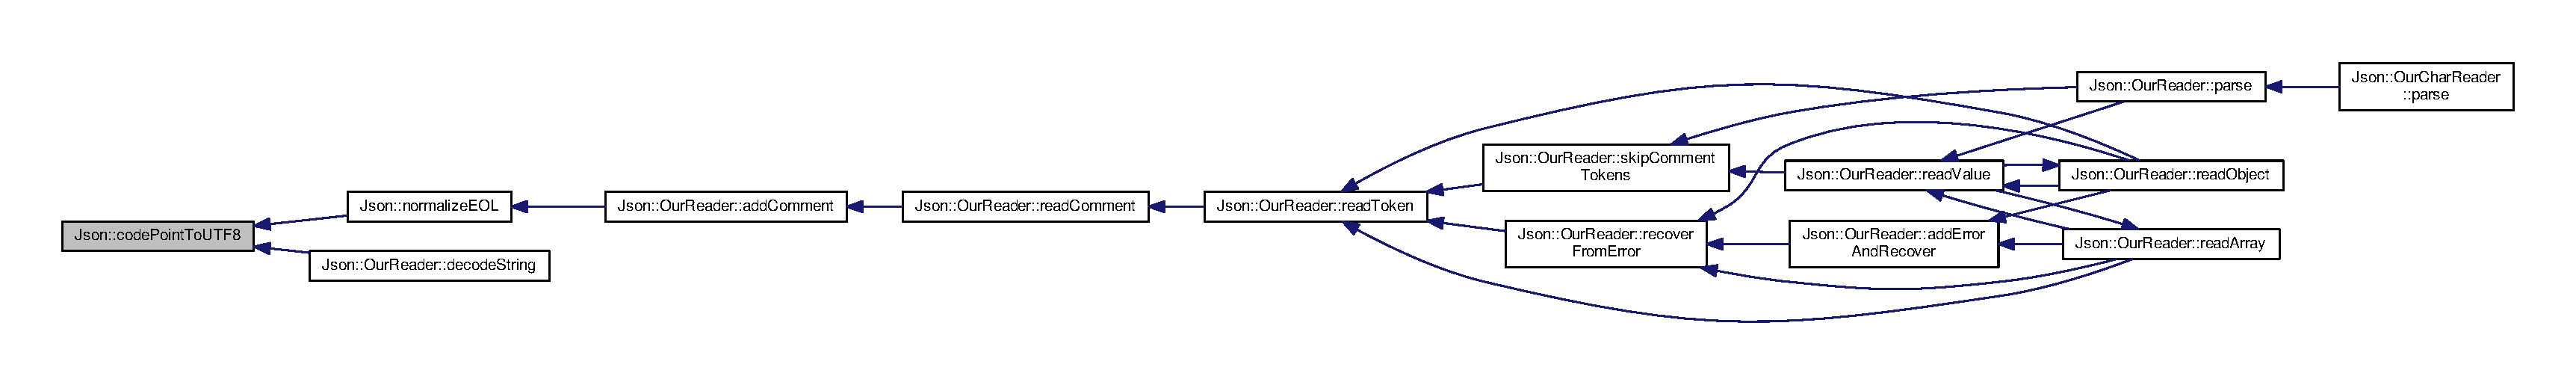
\includegraphics[width=350pt]{namespace_json_adf0456e397a18cd7218a7b51dfc13c73_icgraph}
\end{center}
\end{figure}


\index{Json@{Json}!contains\+Control\+Character@{contains\+Control\+Character}}
\index{contains\+Control\+Character@{contains\+Control\+Character}!Json@{Json}}
\subsubsection[{\texorpdfstring{contains\+Control\+Character(const char $\ast$str)}{containsControlCharacter(const char *str)}}]{\setlength{\rightskip}{0pt plus 5cm}static bool Json\+::contains\+Control\+Character (
\begin{DoxyParamCaption}
\item[{const char $\ast$}]{str}
\end{DoxyParamCaption}
)\hspace{0.3cm}{\ttfamily [static]}}\hypertarget{namespace_json_aa11b210ff98a4f4dd4e2df19260f8c3a}{}\label{namespace_json_aa11b210ff98a4f4dd4e2df19260f8c3a}


Definition at line 4062 of file jsoncpp.\+cpp.



Here is the call graph for this function\+:\nopagebreak
\begin{figure}[H]
\begin{center}
\leavevmode
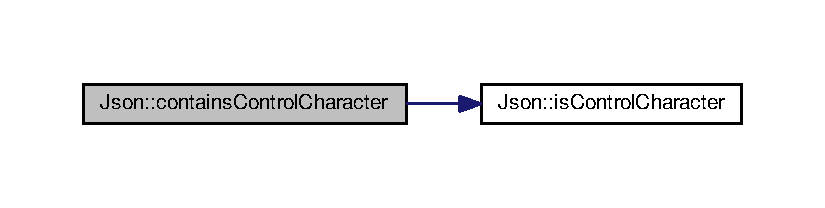
\includegraphics[width=350pt]{namespace_json_aa11b210ff98a4f4dd4e2df19260f8c3a_cgraph}
\end{center}
\end{figure}




Here is the caller graph for this function\+:\nopagebreak
\begin{figure}[H]
\begin{center}
\leavevmode
\includegraphics[width=350pt]{namespace_json_aa11b210ff98a4f4dd4e2df19260f8c3a_icgraph}
\end{center}
\end{figure}


\index{Json@{Json}!contains\+Control\+Character0@{contains\+Control\+Character0}}
\index{contains\+Control\+Character0@{contains\+Control\+Character0}!Json@{Json}}
\subsubsection[{\texorpdfstring{contains\+Control\+Character0(const char $\ast$str, unsigned len)}{containsControlCharacter0(const char *str, unsigned len)}}]{\setlength{\rightskip}{0pt plus 5cm}static bool Json\+::contains\+Control\+Character0 (
\begin{DoxyParamCaption}
\item[{const char $\ast$}]{str, }
\item[{unsigned}]{len}
\end{DoxyParamCaption}
)\hspace{0.3cm}{\ttfamily [static]}}\hypertarget{namespace_json_ae8a357381f264cf28f46449e79ab1dea}{}\label{namespace_json_ae8a357381f264cf28f46449e79ab1dea}


Definition at line 4070 of file jsoncpp.\+cpp.



Here is the call graph for this function\+:\nopagebreak
\begin{figure}[H]
\begin{center}
\leavevmode
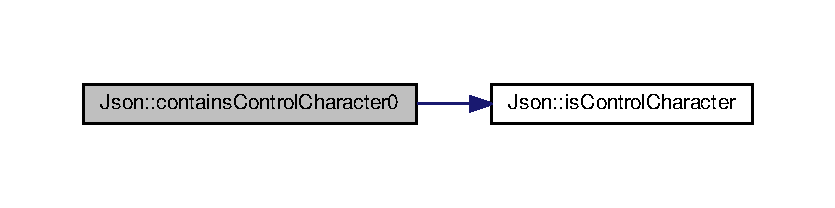
\includegraphics[width=350pt]{namespace_json_ae8a357381f264cf28f46449e79ab1dea_cgraph}
\end{center}
\end{figure}




Here is the caller graph for this function\+:\nopagebreak
\begin{figure}[H]
\begin{center}
\leavevmode
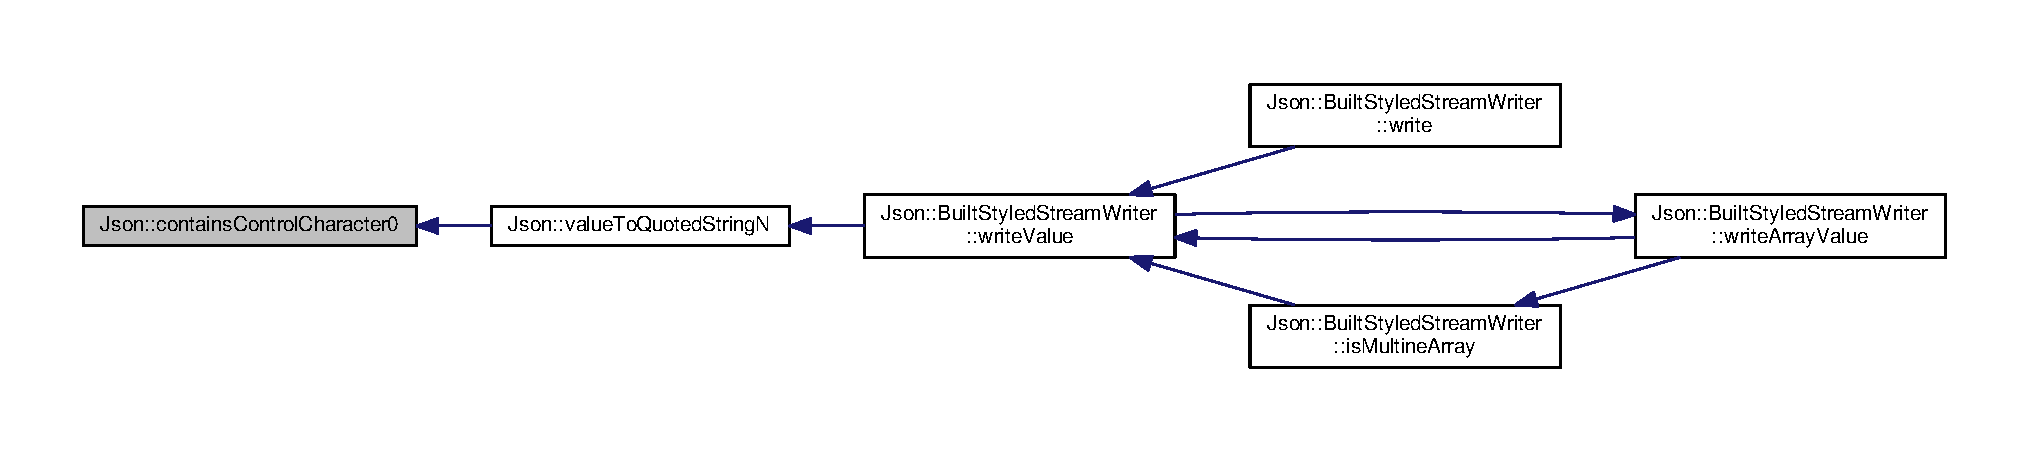
\includegraphics[width=350pt]{namespace_json_ae8a357381f264cf28f46449e79ab1dea_icgraph}
\end{center}
\end{figure}


\index{Json@{Json}!contains\+New\+Line@{contains\+New\+Line}}
\index{contains\+New\+Line@{contains\+New\+Line}!Json@{Json}}
\subsubsection[{\texorpdfstring{contains\+New\+Line(\+Reader\+::\+Location begin, Reader\+::\+Location end)}{containsNewLine(Reader::Location begin, Reader::Location end)}}]{\setlength{\rightskip}{0pt plus 5cm}static bool Json\+::contains\+New\+Line (
\begin{DoxyParamCaption}
\item[{Reader\+::\+Location}]{begin, }
\item[{Reader\+::\+Location}]{end}
\end{DoxyParamCaption}
)\hspace{0.3cm}{\ttfamily [static]}}\hypertarget{namespace_json_a4d6ab0f651348832e5cc49b577a854d2}{}\label{namespace_json_a4d6ab0f651348832e5cc49b577a854d2}


Definition at line 266 of file jsoncpp.\+cpp.



Here is the call graph for this function\+:\nopagebreak
\begin{figure}[H]
\begin{center}
\leavevmode
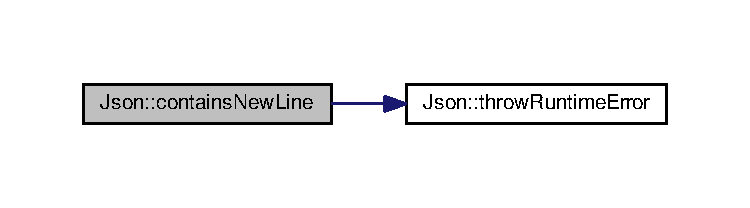
\includegraphics[width=350pt]{namespace_json_a4d6ab0f651348832e5cc49b577a854d2_cgraph}
\end{center}
\end{figure}




Here is the caller graph for this function\+:\nopagebreak
\begin{figure}[H]
\begin{center}
\leavevmode
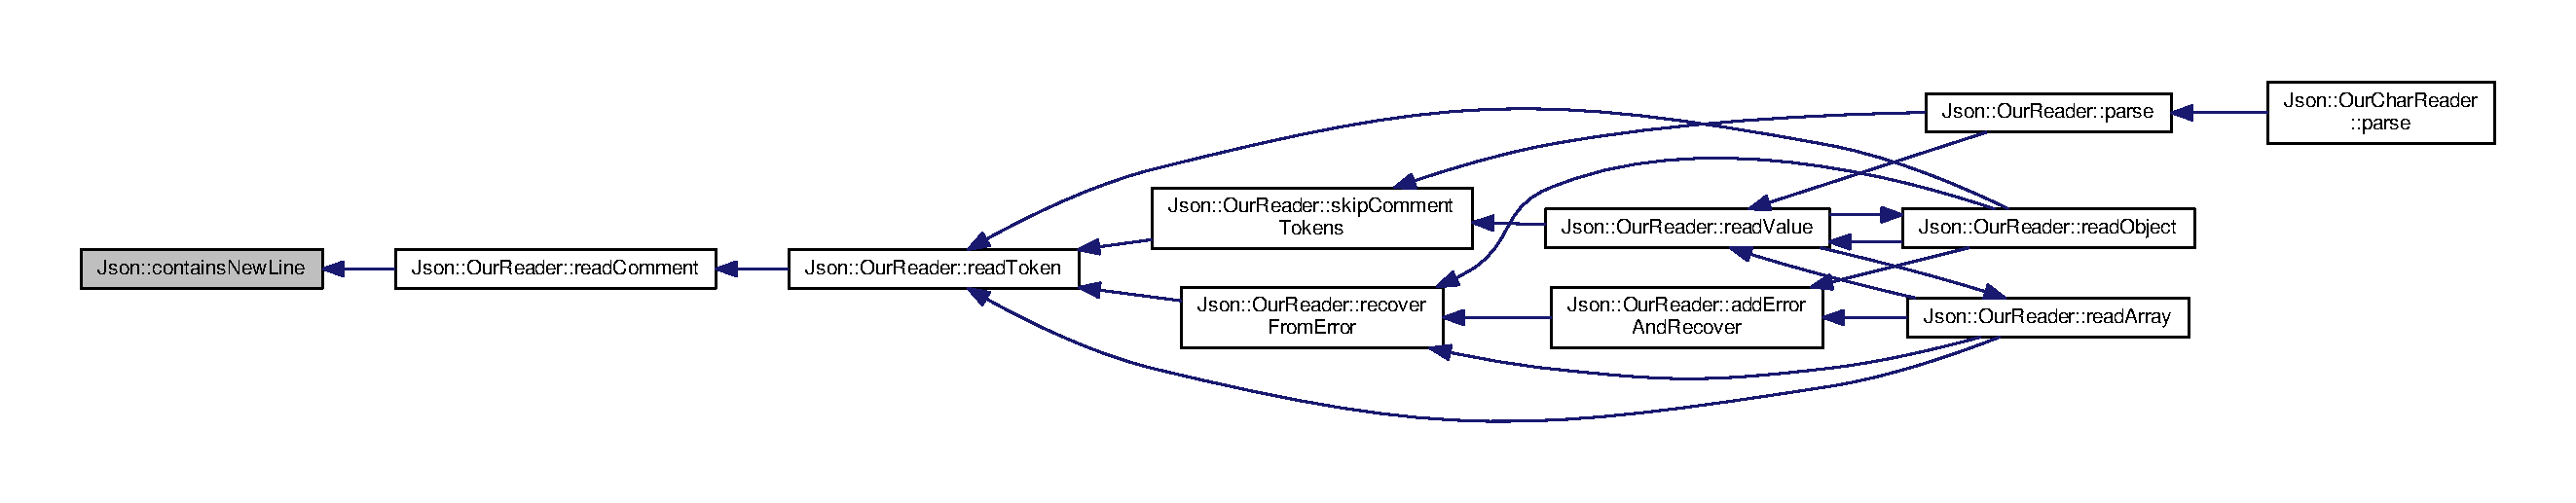
\includegraphics[width=350pt]{namespace_json_a4d6ab0f651348832e5cc49b577a854d2_icgraph}
\end{center}
\end{figure}


\index{Json@{Json}!decode\+Prefixed\+String@{decode\+Prefixed\+String}}
\index{decode\+Prefixed\+String@{decode\+Prefixed\+String}!Json@{Json}}
\subsubsection[{\texorpdfstring{decode\+Prefixed\+String(bool is\+Prefixed, char const $\ast$prefixed, unsigned $\ast$length, char const $\ast$$\ast$value)}{decodePrefixedString(bool isPrefixed, char const *prefixed, unsigned *length, char const **value)}}]{\setlength{\rightskip}{0pt plus 5cm}static void Json\+::decode\+Prefixed\+String (
\begin{DoxyParamCaption}
\item[{bool}]{is\+Prefixed, }
\item[{char const $\ast$}]{prefixed, }
\item[{unsigned $\ast$}]{length, }
\item[{char const $\ast$$\ast$}]{value}
\end{DoxyParamCaption}
)\hspace{0.3cm}{\ttfamily [inline]}, {\ttfamily [static]}}\hypertarget{namespace_json_aad8b4982c1acd164f541fba396ac9fb1}{}\label{namespace_json_aad8b4982c1acd164f541fba396ac9fb1}


Definition at line 2545 of file jsoncpp.\+cpp.



Here is the caller graph for this function\+:\nopagebreak
\begin{figure}[H]
\begin{center}
\leavevmode
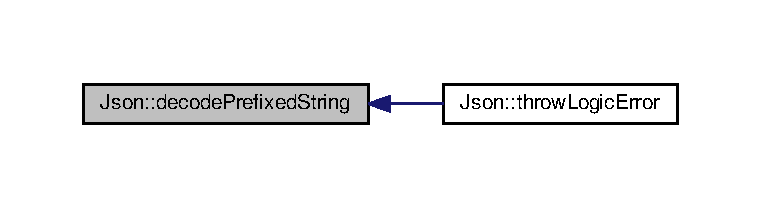
\includegraphics[width=350pt]{namespace_json_aad8b4982c1acd164f541fba396ac9fb1_icgraph}
\end{center}
\end{figure}


\index{Json@{Json}!duplicate\+And\+Prefix\+String\+Value@{duplicate\+And\+Prefix\+String\+Value}}
\index{duplicate\+And\+Prefix\+String\+Value@{duplicate\+And\+Prefix\+String\+Value}!Json@{Json}}
\subsubsection[{\texorpdfstring{duplicate\+And\+Prefix\+String\+Value(const char $\ast$value, unsigned int length)}{duplicateAndPrefixStringValue(const char *value, unsigned int length)}}]{\setlength{\rightskip}{0pt plus 5cm}static char$\ast$ Json\+::duplicate\+And\+Prefix\+String\+Value (
\begin{DoxyParamCaption}
\item[{const char $\ast$}]{value, }
\item[{unsigned int}]{length}
\end{DoxyParamCaption}
)\hspace{0.3cm}{\ttfamily [inline]}, {\ttfamily [static]}}\hypertarget{namespace_json_a9795a09a0141d1f12d307c4386aeaee6}{}\label{namespace_json_a9795a09a0141d1f12d307c4386aeaee6}


Definition at line 2524 of file jsoncpp.\+cpp.



Here is the call graph for this function\+:\nopagebreak
\begin{figure}[H]
\begin{center}
\leavevmode
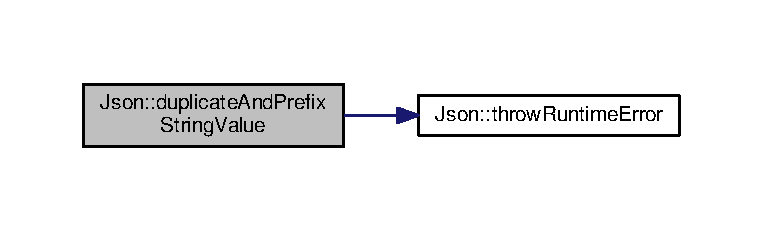
\includegraphics[width=350pt]{namespace_json_a9795a09a0141d1f12d307c4386aeaee6_cgraph}
\end{center}
\end{figure}




Here is the caller graph for this function\+:\nopagebreak
\begin{figure}[H]
\begin{center}
\leavevmode
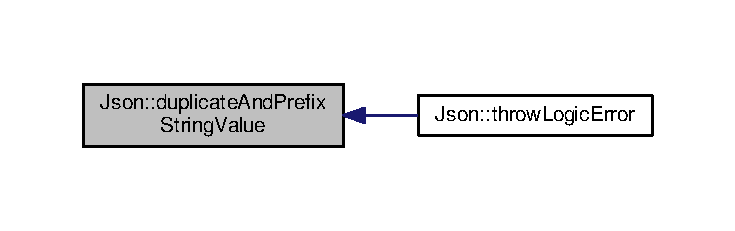
\includegraphics[width=350pt]{namespace_json_a9795a09a0141d1f12d307c4386aeaee6_icgraph}
\end{center}
\end{figure}


\index{Json@{Json}!duplicate\+String\+Value@{duplicate\+String\+Value}}
\index{duplicate\+String\+Value@{duplicate\+String\+Value}!Json@{Json}}
\subsubsection[{\texorpdfstring{duplicate\+String\+Value(const char $\ast$value, size\+\_\+t length)}{duplicateStringValue(const char *value, size_t length)}}]{\setlength{\rightskip}{0pt plus 5cm}static char$\ast$ Json\+::duplicate\+String\+Value (
\begin{DoxyParamCaption}
\item[{const char $\ast$}]{value, }
\item[{size\+\_\+t}]{length}
\end{DoxyParamCaption}
)\hspace{0.3cm}{\ttfamily [inline]}, {\ttfamily [static]}}\hypertarget{namespace_json_a678ac3a60cd70ec0fb4c9abfd40eb0c4}{}\label{namespace_json_a678ac3a60cd70ec0fb4c9abfd40eb0c4}
Duplicates the specified string value. 
\begin{DoxyParams}{Parameters}
{\em value} & Pointer to the string to duplicate. Must be zero-\/terminated if length is \char`\"{}unknown\char`\"{}. \\
\hline
{\em length} & Length of the value. if equals to unknown, then it will be computed using strlen(value). \\
\hline
\end{DoxyParams}
\begin{DoxyReturn}{Returns}
Pointer on the duplicate instance of string. 
\end{DoxyReturn}


Definition at line 2504 of file jsoncpp.\+cpp.



Here is the call graph for this function\+:\nopagebreak
\begin{figure}[H]
\begin{center}
\leavevmode
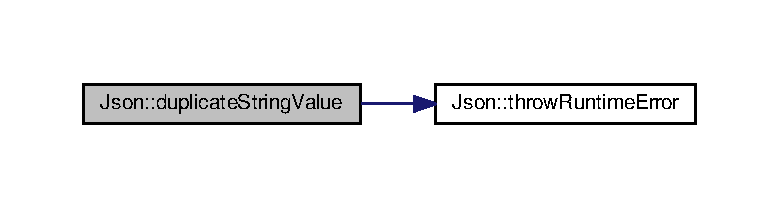
\includegraphics[width=350pt]{namespace_json_a678ac3a60cd70ec0fb4c9abfd40eb0c4_cgraph}
\end{center}
\end{figure}




Here is the caller graph for this function\+:\nopagebreak
\begin{figure}[H]
\begin{center}
\leavevmode
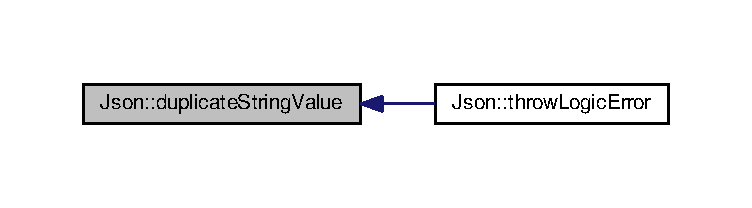
\includegraphics[width=350pt]{namespace_json_a678ac3a60cd70ec0fb4c9abfd40eb0c4_icgraph}
\end{center}
\end{figure}


\index{Json@{Json}!fix\+Numeric\+Locale@{fix\+Numeric\+Locale}}
\index{fix\+Numeric\+Locale@{fix\+Numeric\+Locale}!Json@{Json}}
\subsubsection[{\texorpdfstring{fix\+Numeric\+Locale(char $\ast$begin, char $\ast$end)}{fixNumericLocale(char *begin, char *end)}}]{\setlength{\rightskip}{0pt plus 5cm}static void Json\+::fix\+Numeric\+Locale (
\begin{DoxyParamCaption}
\item[{char $\ast$}]{begin, }
\item[{char $\ast$}]{end}
\end{DoxyParamCaption}
)\hspace{0.3cm}{\ttfamily [inline]}, {\ttfamily [static]}}\hypertarget{namespace_json_aa208904144dc7b11ccc28f47c9afab9a}{}\label{namespace_json_aa208904144dc7b11ccc28f47c9afab9a}
Change \textquotesingle{},\textquotesingle{} to \textquotesingle{}.\textquotesingle{} everywhere in buffer.

We had a sophisticated way, but it did not work in Win\+CE. \begin{DoxySeeAlso}{See also}
\href{https://github.com/open-source-parsers/jsoncpp/pull/9}{\tt https\+://github.\+com/open-\/source-\/parsers/jsoncpp/pull/9} 
\end{DoxySeeAlso}


Definition at line 162 of file jsoncpp.\+cpp.



Here is the caller graph for this function\+:\nopagebreak
\begin{figure}[H]
\begin{center}
\leavevmode
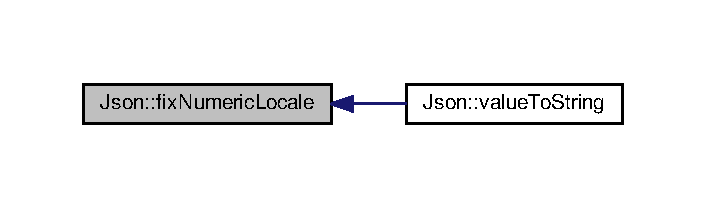
\includegraphics[width=339pt]{namespace_json_aa208904144dc7b11ccc28f47c9afab9a_icgraph}
\end{center}
\end{figure}


\index{Json@{Json}!get\+Valid\+Reader\+Keys@{get\+Valid\+Reader\+Keys}}
\index{get\+Valid\+Reader\+Keys@{get\+Valid\+Reader\+Keys}!Json@{Json}}
\subsubsection[{\texorpdfstring{get\+Valid\+Reader\+Keys(std\+::set$<$ std\+::string $>$ $\ast$valid\+\_\+keys)}{getValidReaderKeys(std::set< std::string > *valid_keys)}}]{\setlength{\rightskip}{0pt plus 5cm}static void Json\+::get\+Valid\+Reader\+Keys (
\begin{DoxyParamCaption}
\item[{std\+::set$<$ std\+::string $>$ $\ast$}]{valid\+\_\+keys}
\end{DoxyParamCaption}
)\hspace{0.3cm}{\ttfamily [static]}}\hypertarget{namespace_json_a8fedd83f49c9a9109d503b2b1d4824aa}{}\label{namespace_json_a8fedd83f49c9a9109d503b2b1d4824aa}


Definition at line 2126 of file jsoncpp.\+cpp.

\index{Json@{Json}!get\+Valid\+Writer\+Keys@{get\+Valid\+Writer\+Keys}}
\index{get\+Valid\+Writer\+Keys@{get\+Valid\+Writer\+Keys}!Json@{Json}}
\subsubsection[{\texorpdfstring{get\+Valid\+Writer\+Keys(std\+::set$<$ std\+::string $>$ $\ast$valid\+\_\+keys)}{getValidWriterKeys(std::set< std::string > *valid_keys)}}]{\setlength{\rightskip}{0pt plus 5cm}static void Json\+::get\+Valid\+Writer\+Keys (
\begin{DoxyParamCaption}
\item[{std\+::set$<$ std\+::string $>$ $\ast$}]{valid\+\_\+keys}
\end{DoxyParamCaption}
)\hspace{0.3cm}{\ttfamily [static]}}\hypertarget{namespace_json_a45c3c8847f03b09cd61035e615d1d820}{}\label{namespace_json_a45c3c8847f03b09cd61035e615d1d820}


Definition at line 5136 of file jsoncpp.\+cpp.

\index{Json@{Json}!In\+Range@{In\+Range}}
\index{In\+Range@{In\+Range}!Json@{Json}}
\subsubsection[{\texorpdfstring{In\+Range(double d, T min, U max)}{InRange(double d, T min, U max)}}]{\setlength{\rightskip}{0pt plus 5cm}template$<$typename T , typename U $>$ static bool Json\+::\+In\+Range (
\begin{DoxyParamCaption}
\item[{double}]{d, }
\item[{T}]{min, }
\item[{U}]{max}
\end{DoxyParamCaption}
)\hspace{0.3cm}{\ttfamily [inline]}, {\ttfamily [static]}}\hypertarget{namespace_json_aff0180507262a244de61b961178d7443}{}\label{namespace_json_aff0180507262a244de61b961178d7443}


Definition at line 2476 of file jsoncpp.\+cpp.



Here is the caller graph for this function\+:\nopagebreak
\begin{figure}[H]
\begin{center}
\leavevmode
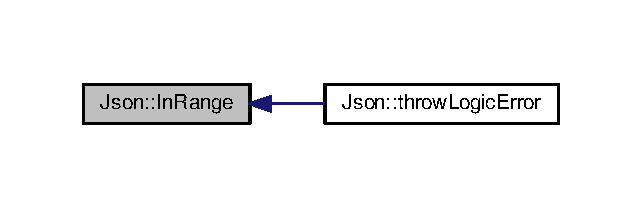
\includegraphics[width=308pt]{namespace_json_aff0180507262a244de61b961178d7443_icgraph}
\end{center}
\end{figure}


\index{Json@{Json}!is\+Control\+Character@{is\+Control\+Character}}
\index{is\+Control\+Character@{is\+Control\+Character}!Json@{Json}}
\subsubsection[{\texorpdfstring{is\+Control\+Character(char ch)}{isControlCharacter(char ch)}}]{\setlength{\rightskip}{0pt plus 5cm}static bool Json\+::is\+Control\+Character (
\begin{DoxyParamCaption}
\item[{char}]{ch}
\end{DoxyParamCaption}
)\hspace{0.3cm}{\ttfamily [inline]}, {\ttfamily [static]}}\hypertarget{namespace_json_a0381e631737f51331065a388f4f59197}{}\label{namespace_json_a0381e631737f51331065a388f4f59197}


Returns true if ch is a control character (in range \mbox{[}1,31\mbox{]}). 



Definition at line 133 of file jsoncpp.\+cpp.



Here is the caller graph for this function\+:\nopagebreak
\begin{figure}[H]
\begin{center}
\leavevmode
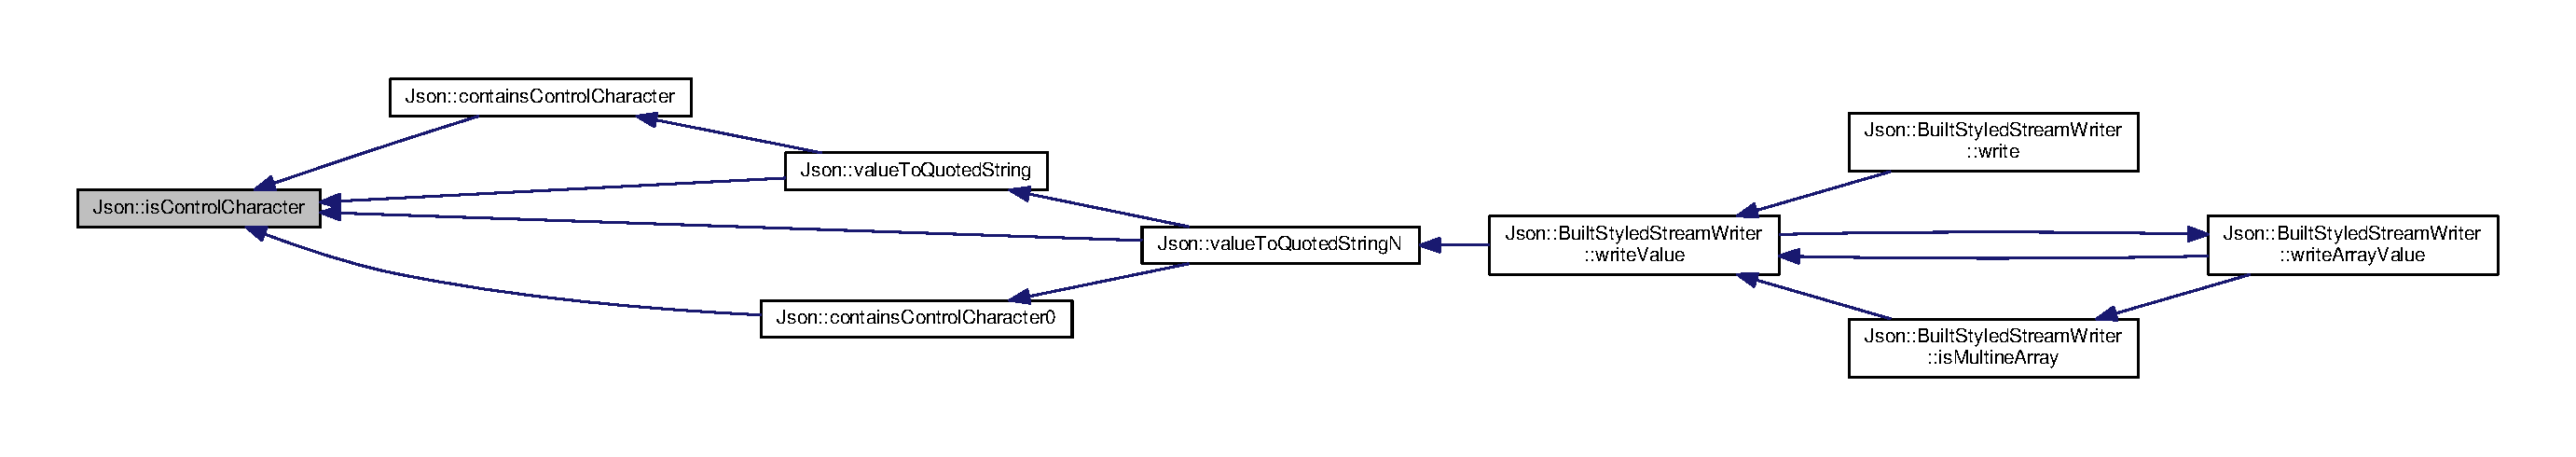
\includegraphics[width=350pt]{namespace_json_a0381e631737f51331065a388f4f59197_icgraph}
\end{center}
\end{figure}


\index{Json@{Json}!Is\+Integral@{Is\+Integral}}
\index{Is\+Integral@{Is\+Integral}!Json@{Json}}
\subsubsection[{\texorpdfstring{Is\+Integral(double d)}{IsIntegral(double d)}}]{\setlength{\rightskip}{0pt plus 5cm}static bool Json\+::\+Is\+Integral (
\begin{DoxyParamCaption}
\item[{double}]{d}
\end{DoxyParamCaption}
)\hspace{0.3cm}{\ttfamily [static]}}\hypertarget{namespace_json_a1a04cc9d31e64b5912dade003c9b99b5}{}\label{namespace_json_a1a04cc9d31e64b5912dade003c9b99b5}


Definition at line 3633 of file jsoncpp.\+cpp.

\index{Json@{Json}!normalize\+E\+OL@{normalize\+E\+OL}}
\index{normalize\+E\+OL@{normalize\+E\+OL}!Json@{Json}}
\subsubsection[{\texorpdfstring{normalize\+E\+O\+L(\+Reader\+::\+Location begin, Reader\+::\+Location end)}{normalizeEOL(Reader::Location begin, Reader::Location end)}}]{\setlength{\rightskip}{0pt plus 5cm}static std\+::string Json\+::normalize\+E\+OL (
\begin{DoxyParamCaption}
\item[{Reader\+::\+Location}]{begin, }
\item[{Reader\+::\+Location}]{end}
\end{DoxyParamCaption}
)\hspace{0.3cm}{\ttfamily [static]}}\hypertarget{namespace_json_a2e6b8616041876128cbef54b8c75da62}{}\label{namespace_json_a2e6b8616041876128cbef54b8c75da62}


Definition at line 558 of file jsoncpp.\+cpp.



Here is the call graph for this function\+:\nopagebreak
\begin{figure}[H]
\begin{center}
\leavevmode
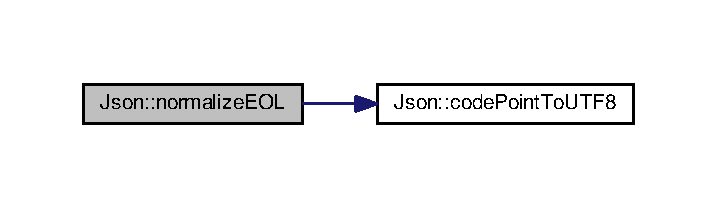
\includegraphics[width=344pt]{namespace_json_a2e6b8616041876128cbef54b8c75da62_cgraph}
\end{center}
\end{figure}




Here is the caller graph for this function\+:\nopagebreak
\begin{figure}[H]
\begin{center}
\leavevmode
\includegraphics[width=350pt]{namespace_json_a2e6b8616041876128cbef54b8c75da62_icgraph}
\end{center}
\end{figure}


\index{Json@{Json}!operator$<$$<$@{operator$<$$<$}}
\index{operator$<$$<$@{operator$<$$<$}!Json@{Json}}
\subsubsection[{\texorpdfstring{operator$<$$<$(std\+::ostream \&sout, Value const \&root)}{operator<<(std::ostream &sout, Value const &root)}}]{\setlength{\rightskip}{0pt plus 5cm}std\+::ostream\& Json\+::operator$<$$<$ (
\begin{DoxyParamCaption}
\item[{std\+::ostream \&}]{sout, }
\item[{Value const \&}]{root}
\end{DoxyParamCaption}
)}\hypertarget{namespace_json_af64fba09a9679b8b8cb50dd3e85f6fd5}{}\label{namespace_json_af64fba09a9679b8b8cb50dd3e85f6fd5}


Definition at line 5187 of file jsoncpp.\+cpp.

\index{Json@{Json}!operator$>$$>$@{operator$>$$>$}}
\index{operator$>$$>$@{operator$>$$>$}!Json@{Json}}
\subsubsection[{\texorpdfstring{operator$>$$>$(std\+::istream \&sin, Value \&root)}{operator>>(std::istream &sin, Value &root)}}]{\setlength{\rightskip}{0pt plus 5cm}std\+::istream\& Json\+::operator$>$$>$ (
\begin{DoxyParamCaption}
\item[{std\+::istream \&}]{sin, }
\item[{Value \&}]{root}
\end{DoxyParamCaption}
)}\hypertarget{namespace_json_a2434499c0c7f057890b32787c05fc4a3}{}\label{namespace_json_a2434499c0c7f057890b32787c05fc4a3}


Definition at line 2210 of file jsoncpp.\+cpp.



Here is the call graph for this function\+:\nopagebreak
\begin{figure}[H]
\begin{center}
\leavevmode
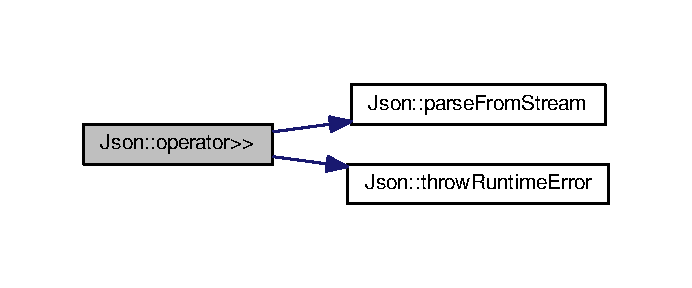
\includegraphics[width=332pt]{namespace_json_a2434499c0c7f057890b32787c05fc4a3_cgraph}
\end{center}
\end{figure}


\index{Json@{Json}!parse\+From\+Stream@{parse\+From\+Stream}}
\index{parse\+From\+Stream@{parse\+From\+Stream}!Json@{Json}}
\subsubsection[{\texorpdfstring{parse\+From\+Stream(\+Char\+Reader\+::\+Factory const \&fact, std\+::istream \&sin, Value $\ast$root, std\+::string $\ast$errs)}{parseFromStream(CharReader::Factory const &fact, std::istream &sin, Value *root, std::string *errs)}}]{\setlength{\rightskip}{0pt plus 5cm}bool Json\+::parse\+From\+Stream (
\begin{DoxyParamCaption}
\item[{Char\+Reader\+::\+Factory const \&}]{fact, }
\item[{std\+::istream \&}]{sin, }
\item[{Value $\ast$}]{root, }
\item[{std\+::string $\ast$}]{errs}
\end{DoxyParamCaption}
)}\hypertarget{namespace_json_a7b90be78407a3a1f241b2a3048ef3d19}{}\label{namespace_json_a7b90be78407a3a1f241b2a3048ef3d19}


Definition at line 2196 of file jsoncpp.\+cpp.



Here is the caller graph for this function\+:\nopagebreak
\begin{figure}[H]
\begin{center}
\leavevmode
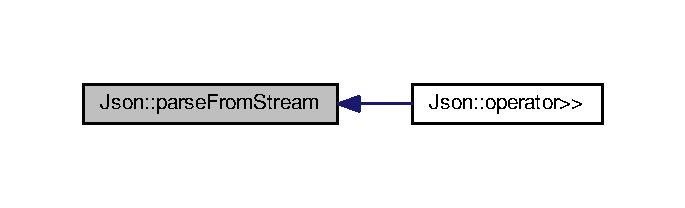
\includegraphics[width=329pt]{namespace_json_a7b90be78407a3a1f241b2a3048ef3d19_icgraph}
\end{center}
\end{figure}


\index{Json@{Json}!release\+String\+Value@{release\+String\+Value}}
\index{release\+String\+Value@{release\+String\+Value}!Json@{Json}}
\subsubsection[{\texorpdfstring{release\+String\+Value(char $\ast$value)}{releaseStringValue(char *value)}}]{\setlength{\rightskip}{0pt plus 5cm}static void Json\+::release\+String\+Value (
\begin{DoxyParamCaption}
\item[{char $\ast$}]{value}
\end{DoxyParamCaption}
)\hspace{0.3cm}{\ttfamily [inline]}, {\ttfamily [static]}}\hypertarget{namespace_json_acf8dd162c01e37846e129556c50e4037}{}\label{namespace_json_acf8dd162c01e37846e129556c50e4037}
Free the string duplicated by \hyperlink{namespace_json_a678ac3a60cd70ec0fb4c9abfd40eb0c4}{duplicate\+String\+Value()}/duplicate\+And\+Prefix\+String\+Value(). 

Definition at line 2559 of file jsoncpp.\+cpp.



Here is the caller graph for this function\+:\nopagebreak
\begin{figure}[H]
\begin{center}
\leavevmode
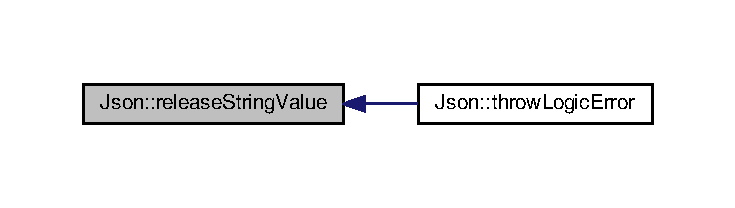
\includegraphics[width=350pt]{namespace_json_acf8dd162c01e37846e129556c50e4037_icgraph}
\end{center}
\end{figure}


\index{Json@{Json}!strnpbrk@{strnpbrk}}
\index{strnpbrk@{strnpbrk}!Json@{Json}}
\subsubsection[{\texorpdfstring{strnpbrk(char const $\ast$s, char const $\ast$accept, size\+\_\+t n)}{strnpbrk(char const *s, char const *accept, size_t n)}}]{\setlength{\rightskip}{0pt plus 5cm}static char const$\ast$ Json\+::strnpbrk (
\begin{DoxyParamCaption}
\item[{char const $\ast$}]{s, }
\item[{char const $\ast$}]{accept, }
\item[{size\+\_\+t}]{n}
\end{DoxyParamCaption}
)\hspace{0.3cm}{\ttfamily [static]}}\hypertarget{namespace_json_a7492156d0c7d2dd2f672acacfb240320}{}\label{namespace_json_a7492156d0c7d2dd2f672acacfb240320}


Definition at line 4213 of file jsoncpp.\+cpp.



Here is the caller graph for this function\+:\nopagebreak
\begin{figure}[H]
\begin{center}
\leavevmode
\includegraphics[width=350pt]{namespace_json_a7492156d0c7d2dd2f672acacfb240320_icgraph}
\end{center}
\end{figure}


\index{Json@{Json}!throw\+Logic\+Error@{throw\+Logic\+Error}}
\index{throw\+Logic\+Error@{throw\+Logic\+Error}!Json@{Json}}
\subsubsection[{\texorpdfstring{throw\+Logic\+Error(std\+::string const \&msg)}{throwLogicError(std::string const &msg)}}]{\setlength{\rightskip}{0pt plus 5cm}void Json\+::throw\+Logic\+Error (
\begin{DoxyParamCaption}
\item[{std\+::string const \&}]{msg}
\end{DoxyParamCaption}
)}\hypertarget{namespace_json_a27613326e9e36bbfe04a905ac90caa91}{}\label{namespace_json_a27613326e9e36bbfe04a905ac90caa91}


Definition at line 2596 of file jsoncpp.\+cpp.



Here is the call graph for this function\+:\nopagebreak
\begin{figure}[H]
\begin{center}
\leavevmode
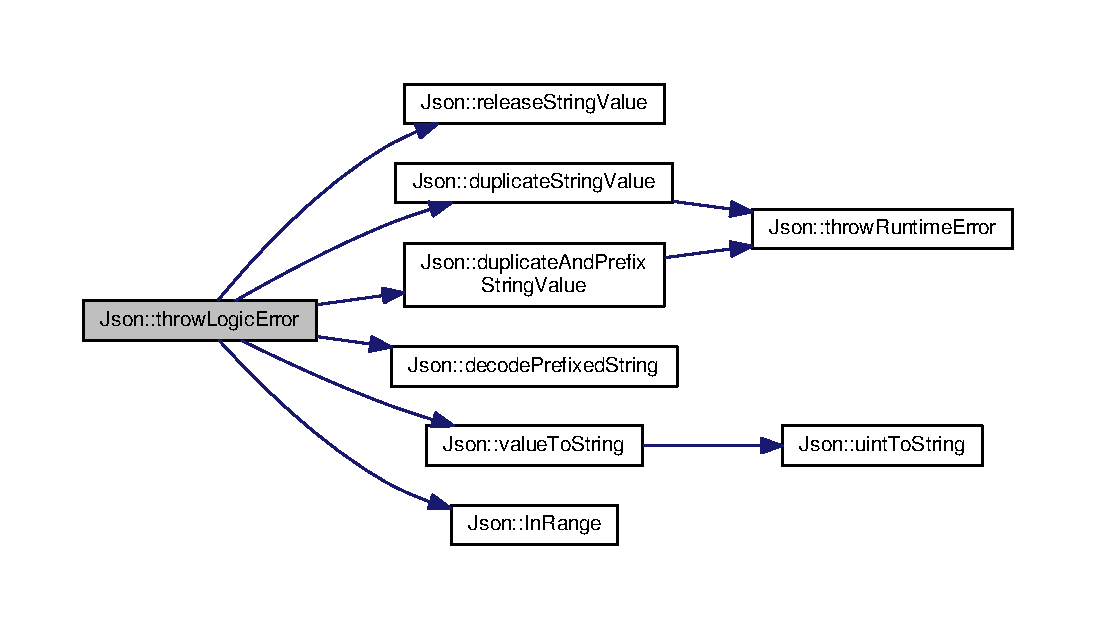
\includegraphics[width=350pt]{namespace_json_a27613326e9e36bbfe04a905ac90caa91_cgraph}
\end{center}
\end{figure}


\index{Json@{Json}!throw\+Runtime\+Error@{throw\+Runtime\+Error}}
\index{throw\+Runtime\+Error@{throw\+Runtime\+Error}!Json@{Json}}
\subsubsection[{\texorpdfstring{throw\+Runtime\+Error(std\+::string const \&msg)}{throwRuntimeError(std::string const &msg)}}]{\setlength{\rightskip}{0pt plus 5cm}void Json\+::throw\+Runtime\+Error (
\begin{DoxyParamCaption}
\item[{std\+::string const \&}]{msg}
\end{DoxyParamCaption}
)}\hypertarget{namespace_json_a97f039a107b3f6cf1c3edee50e978f76}{}\label{namespace_json_a97f039a107b3f6cf1c3edee50e978f76}


Definition at line 2592 of file jsoncpp.\+cpp.



Here is the caller graph for this function\+:\nopagebreak
\begin{figure}[H]
\begin{center}
\leavevmode
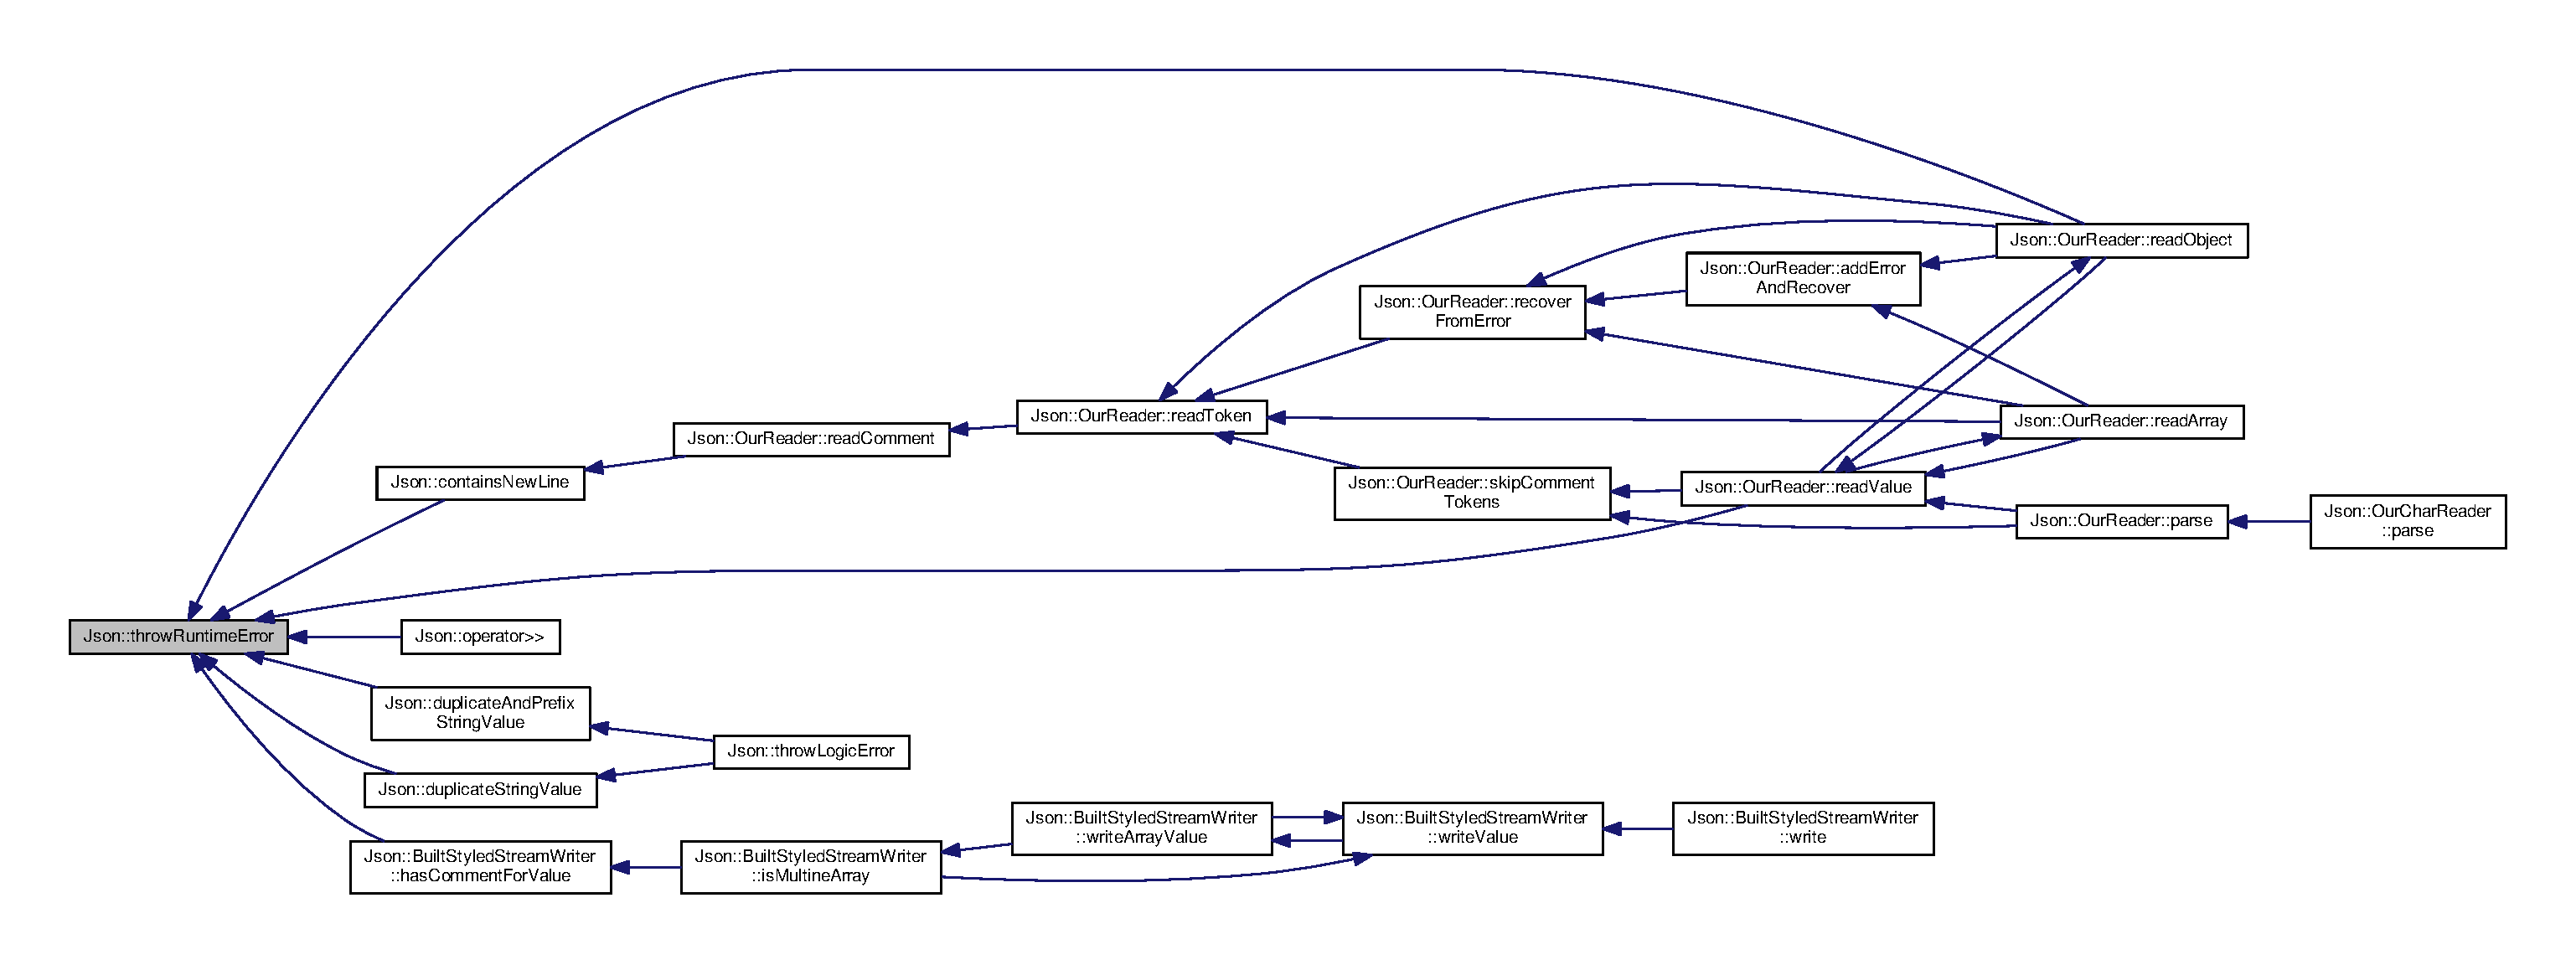
\includegraphics[width=350pt]{namespace_json_a97f039a107b3f6cf1c3edee50e978f76_icgraph}
\end{center}
\end{figure}


\index{Json@{Json}!uint\+To\+String@{uint\+To\+String}}
\index{uint\+To\+String@{uint\+To\+String}!Json@{Json}}
\subsubsection[{\texorpdfstring{uint\+To\+String(\+Largest\+U\+Int value, char $\ast$\&current)}{uintToString(LargestUInt value, char *&current)}}]{\setlength{\rightskip}{0pt plus 5cm}static void Json\+::uint\+To\+String (
\begin{DoxyParamCaption}
\item[{Largest\+U\+Int}]{value, }
\item[{char $\ast$\&}]{current}
\end{DoxyParamCaption}
)\hspace{0.3cm}{\ttfamily [inline]}, {\ttfamily [static]}}\hypertarget{namespace_json_ac1ffd21a9e55122014353c773ccc496e}{}\label{namespace_json_ac1ffd21a9e55122014353c773ccc496e}
Converts an unsigned integer to string. 
\begin{DoxyParams}{Parameters}
{\em value} & Unsigned interger to convert to string \\
\hline
{\em current} & Input/\+Output string buffer. Must have at least uint\+To\+String\+Buffer\+Size chars free. \\
\hline
\end{DoxyParams}


Definition at line 149 of file jsoncpp.\+cpp.



Here is the caller graph for this function\+:\nopagebreak
\begin{figure}[H]
\begin{center}
\leavevmode
\includegraphics[width=350pt]{namespace_json_ac1ffd21a9e55122014353c773ccc496e_icgraph}
\end{center}
\end{figure}


\index{Json@{Json}!value\+To\+Quoted\+String@{value\+To\+Quoted\+String}}
\index{value\+To\+Quoted\+String@{value\+To\+Quoted\+String}!Json@{Json}}
\subsubsection[{\texorpdfstring{value\+To\+Quoted\+String(const char $\ast$value)}{valueToQuotedString(const char *value)}}]{\setlength{\rightskip}{0pt plus 5cm}std\+::string Json\+::value\+To\+Quoted\+String (
\begin{DoxyParamCaption}
\item[{const char $\ast$}]{value}
\end{DoxyParamCaption}
)}\hypertarget{namespace_json_aa0c8235a4a5c6599da5d3332743db8ac}{}\label{namespace_json_aa0c8235a4a5c6599da5d3332743db8ac}


Definition at line 4150 of file jsoncpp.\+cpp.



Here is the call graph for this function\+:\nopagebreak
\begin{figure}[H]
\begin{center}
\leavevmode
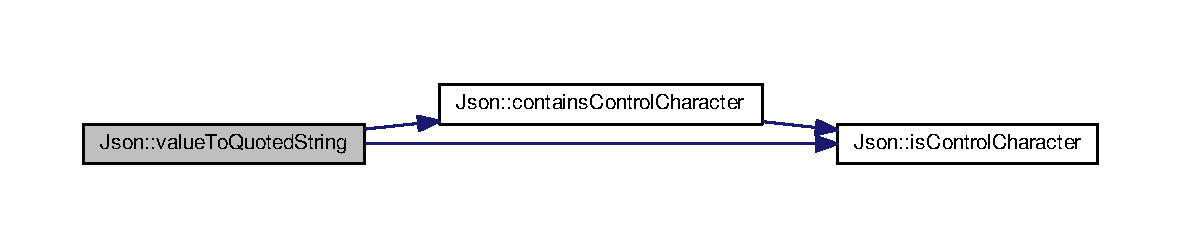
\includegraphics[width=350pt]{namespace_json_aa0c8235a4a5c6599da5d3332743db8ac_cgraph}
\end{center}
\end{figure}




Here is the caller graph for this function\+:\nopagebreak
\begin{figure}[H]
\begin{center}
\leavevmode
\includegraphics[width=350pt]{namespace_json_aa0c8235a4a5c6599da5d3332743db8ac_icgraph}
\end{center}
\end{figure}


\index{Json@{Json}!value\+To\+Quoted\+StringN@{value\+To\+Quoted\+StringN}}
\index{value\+To\+Quoted\+StringN@{value\+To\+Quoted\+StringN}!Json@{Json}}
\subsubsection[{\texorpdfstring{value\+To\+Quoted\+String\+N(const char $\ast$value, unsigned length)}{valueToQuotedStringN(const char *value, unsigned length)}}]{\setlength{\rightskip}{0pt plus 5cm}static std\+::string Json\+::value\+To\+Quoted\+StringN (
\begin{DoxyParamCaption}
\item[{const char $\ast$}]{value, }
\item[{unsigned}]{length}
\end{DoxyParamCaption}
)\hspace{0.3cm}{\ttfamily [static]}}\hypertarget{namespace_json_a20d52b5a457ee5d833645d119451c2cd}{}\label{namespace_json_a20d52b5a457ee5d833645d119451c2cd}


Definition at line 4227 of file jsoncpp.\+cpp.



Here is the call graph for this function\+:\nopagebreak
\begin{figure}[H]
\begin{center}
\leavevmode
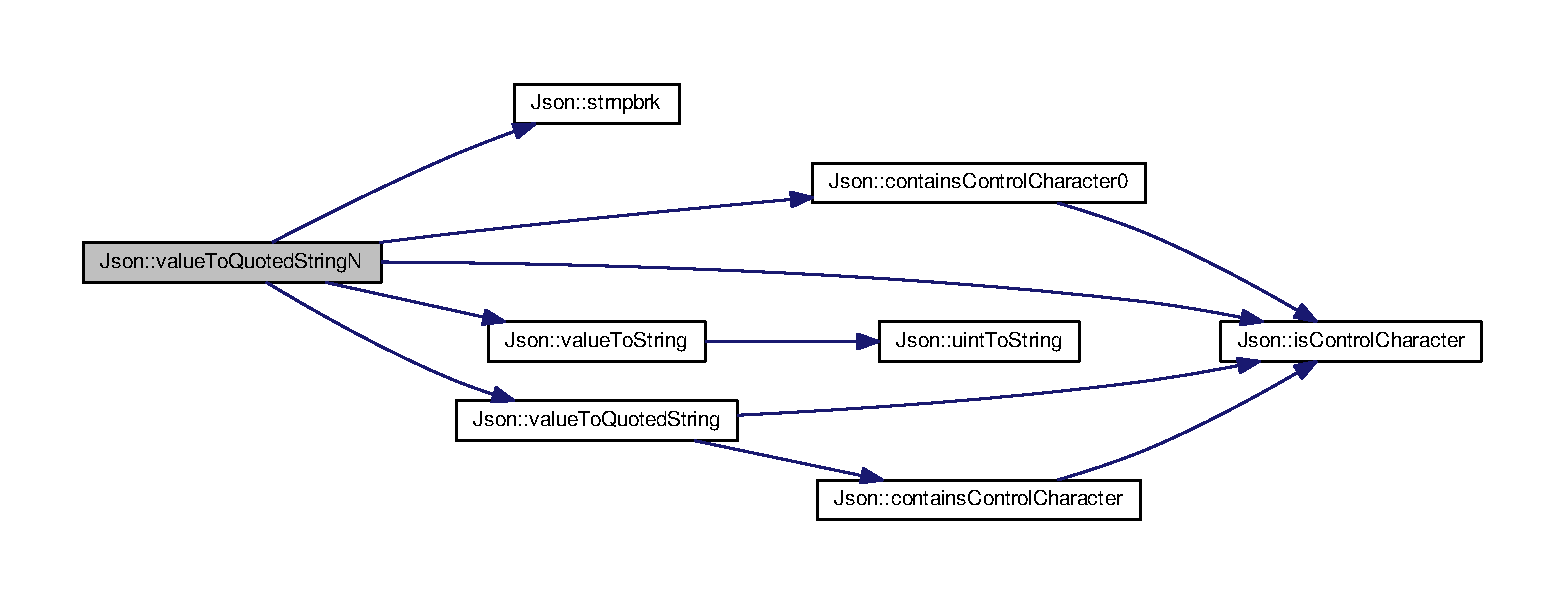
\includegraphics[width=350pt]{namespace_json_a20d52b5a457ee5d833645d119451c2cd_cgraph}
\end{center}
\end{figure}




Here is the caller graph for this function\+:\nopagebreak
\begin{figure}[H]
\begin{center}
\leavevmode
\includegraphics[width=350pt]{namespace_json_a20d52b5a457ee5d833645d119451c2cd_icgraph}
\end{center}
\end{figure}


\index{Json@{Json}!value\+To\+String@{value\+To\+String}}
\index{value\+To\+String@{value\+To\+String}!Json@{Json}}
\subsubsection[{\texorpdfstring{value\+To\+String(\+Largest\+Int value)}{valueToString(LargestInt value)}}]{\setlength{\rightskip}{0pt plus 5cm}std\+::string Json\+::value\+To\+String (
\begin{DoxyParamCaption}
\item[{Largest\+Int}]{value}
\end{DoxyParamCaption}
)}\hypertarget{namespace_json_abd9c650f70d9434f98f9025e2e2faf2d}{}\label{namespace_json_abd9c650f70d9434f98f9025e2e2faf2d}


Definition at line 4080 of file jsoncpp.\+cpp.



Here is the call graph for this function\+:\nopagebreak
\begin{figure}[H]
\begin{center}
\leavevmode
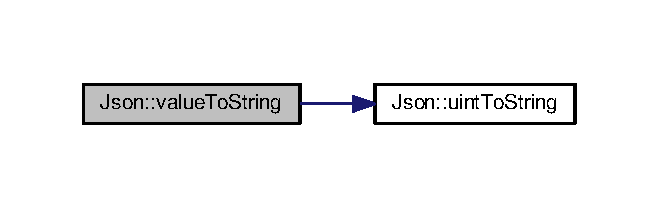
\includegraphics[width=316pt]{namespace_json_abd9c650f70d9434f98f9025e2e2faf2d_cgraph}
\end{center}
\end{figure}




Here is the caller graph for this function\+:\nopagebreak
\begin{figure}[H]
\begin{center}
\leavevmode
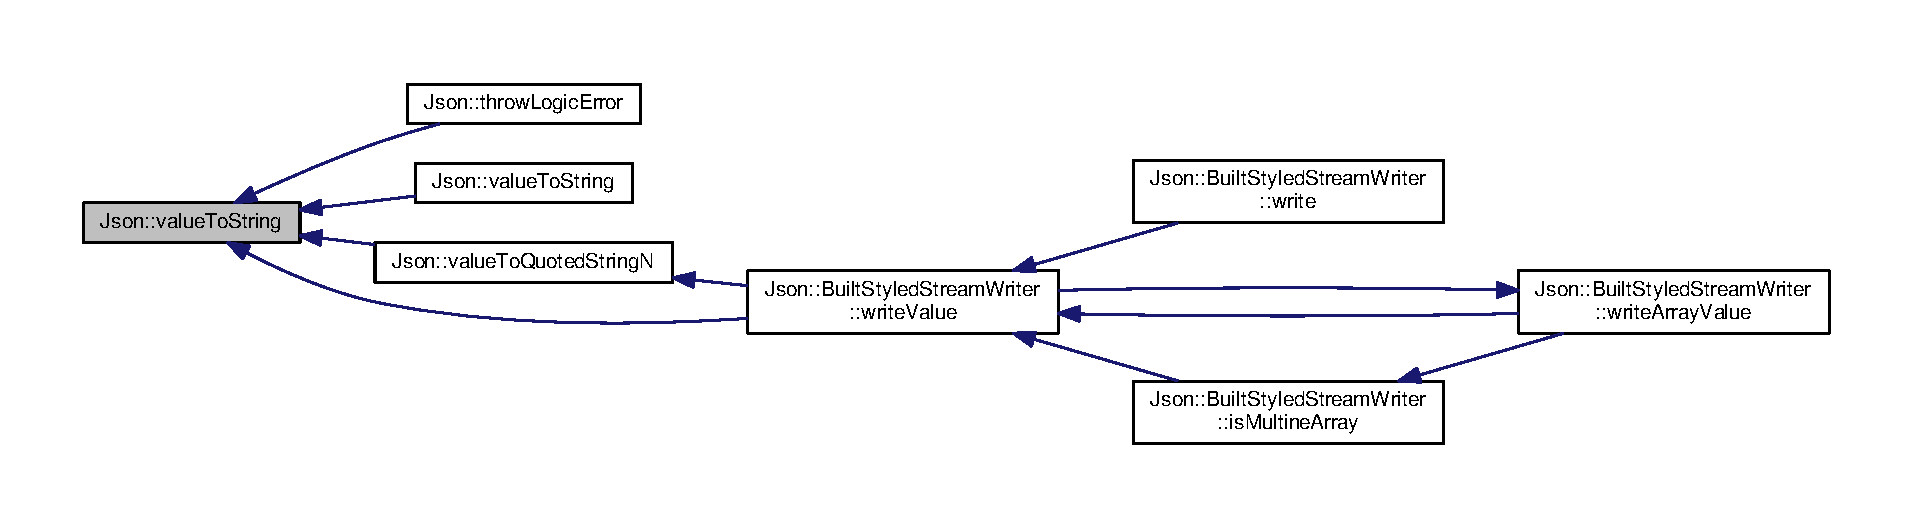
\includegraphics[width=350pt]{namespace_json_abd9c650f70d9434f98f9025e2e2faf2d_icgraph}
\end{center}
\end{figure}


\index{Json@{Json}!value\+To\+String@{value\+To\+String}}
\index{value\+To\+String@{value\+To\+String}!Json@{Json}}
\subsubsection[{\texorpdfstring{value\+To\+String(\+Largest\+U\+Int value)}{valueToString(LargestUInt value)}}]{\setlength{\rightskip}{0pt plus 5cm}std\+::string Json\+::value\+To\+String (
\begin{DoxyParamCaption}
\item[{Largest\+U\+Int}]{value}
\end{DoxyParamCaption}
)}\hypertarget{namespace_json_a3f46b0bc62b95a9426a2da0117bdf9f0}{}\label{namespace_json_a3f46b0bc62b95a9426a2da0117bdf9f0}


Definition at line 4096 of file jsoncpp.\+cpp.



Here is the call graph for this function\+:\nopagebreak
\begin{figure}[H]
\begin{center}
\leavevmode
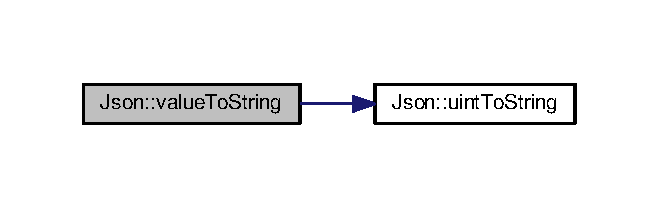
\includegraphics[width=316pt]{namespace_json_a3f46b0bc62b95a9426a2da0117bdf9f0_cgraph}
\end{center}
\end{figure}


\index{Json@{Json}!value\+To\+String@{value\+To\+String}}
\index{value\+To\+String@{value\+To\+String}!Json@{Json}}
\subsubsection[{\texorpdfstring{value\+To\+String(\+Int value)}{valueToString(Int value)}}]{\setlength{\rightskip}{0pt plus 5cm}std\+::string Json\+::value\+To\+String (
\begin{DoxyParamCaption}
\item[{Int}]{value}
\end{DoxyParamCaption}
)}\hypertarget{namespace_json_a5d3eba6789f9a9c1ab563ff8b4a5090f}{}\label{namespace_json_a5d3eba6789f9a9c1ab563ff8b4a5090f}


Definition at line 4106 of file jsoncpp.\+cpp.



Here is the call graph for this function\+:\nopagebreak
\begin{figure}[H]
\begin{center}
\leavevmode
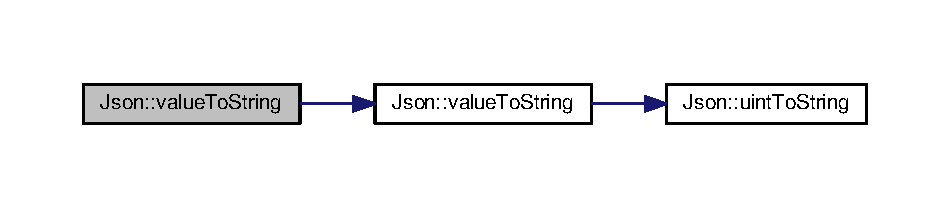
\includegraphics[width=350pt]{namespace_json_a5d3eba6789f9a9c1ab563ff8b4a5090f_cgraph}
\end{center}
\end{figure}


\index{Json@{Json}!value\+To\+String@{value\+To\+String}}
\index{value\+To\+String@{value\+To\+String}!Json@{Json}}
\subsubsection[{\texorpdfstring{value\+To\+String(\+U\+Int value)}{valueToString(UInt value)}}]{\setlength{\rightskip}{0pt plus 5cm}std\+::string Json\+::value\+To\+String (
\begin{DoxyParamCaption}
\item[{U\+Int}]{value}
\end{DoxyParamCaption}
)}\hypertarget{namespace_json_a4d43b0ff222bd3975bcf1babca0b978f}{}\label{namespace_json_a4d43b0ff222bd3975bcf1babca0b978f}


Definition at line 4110 of file jsoncpp.\+cpp.



Here is the call graph for this function\+:\nopagebreak
\begin{figure}[H]
\begin{center}
\leavevmode
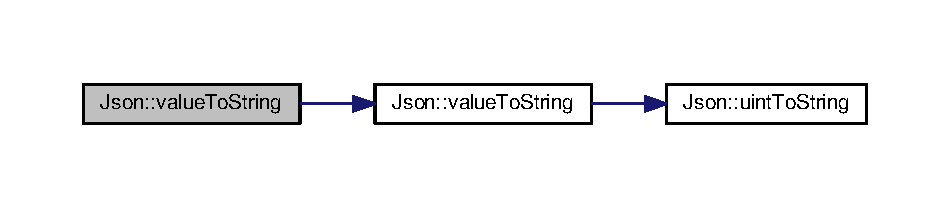
\includegraphics[width=350pt]{namespace_json_a4d43b0ff222bd3975bcf1babca0b978f_cgraph}
\end{center}
\end{figure}


\index{Json@{Json}!value\+To\+String@{value\+To\+String}}
\index{value\+To\+String@{value\+To\+String}!Json@{Json}}
\subsubsection[{\texorpdfstring{value\+To\+String(double value, bool use\+Special\+Floats, unsigned int precision)}{valueToString(double value, bool useSpecialFloats, unsigned int precision)}}]{\setlength{\rightskip}{0pt plus 5cm}std\+::string Json\+::value\+To\+String (
\begin{DoxyParamCaption}
\item[{double}]{value, }
\item[{bool}]{use\+Special\+Floats, }
\item[{unsigned int}]{precision}
\end{DoxyParamCaption}
)}\hypertarget{namespace_json_a1c49ced79060a67638d7fa78a63b1813}{}\label{namespace_json_a1c49ced79060a67638d7fa78a63b1813}


Definition at line 4116 of file jsoncpp.\+cpp.



Here is the call graph for this function\+:\nopagebreak
\begin{figure}[H]
\begin{center}
\leavevmode
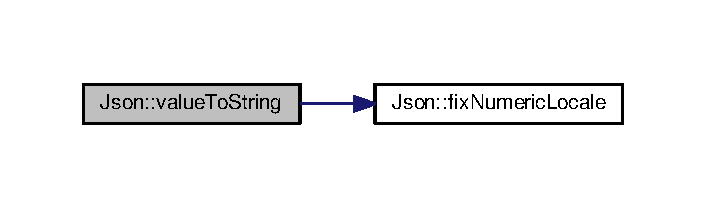
\includegraphics[width=339pt]{namespace_json_a1c49ced79060a67638d7fa78a63b1813_cgraph}
\end{center}
\end{figure}


\index{Json@{Json}!value\+To\+String@{value\+To\+String}}
\index{value\+To\+String@{value\+To\+String}!Json@{Json}}
\subsubsection[{\texorpdfstring{value\+To\+String(double value)}{valueToString(double value)}}]{\setlength{\rightskip}{0pt plus 5cm}std\+::string Json\+::value\+To\+String (
\begin{DoxyParamCaption}
\item[{double}]{value}
\end{DoxyParamCaption}
)}\hypertarget{namespace_json_a99995d7dafa4f4970b349d7d3c8d1d99}{}\label{namespace_json_a99995d7dafa4f4970b349d7d3c8d1d99}


Definition at line 4146 of file jsoncpp.\+cpp.



Here is the call graph for this function\+:\nopagebreak
\begin{figure}[H]
\begin{center}
\leavevmode
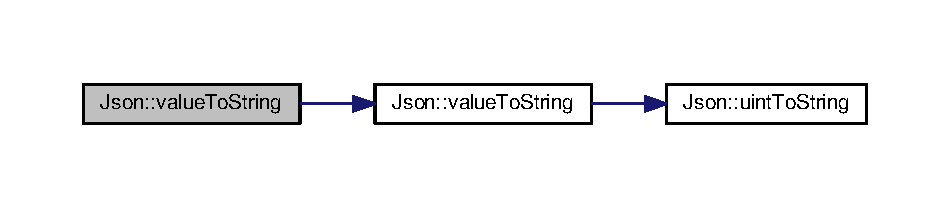
\includegraphics[width=350pt]{namespace_json_a99995d7dafa4f4970b349d7d3c8d1d99_cgraph}
\end{center}
\end{figure}


\index{Json@{Json}!value\+To\+String@{value\+To\+String}}
\index{value\+To\+String@{value\+To\+String}!Json@{Json}}
\subsubsection[{\texorpdfstring{value\+To\+String(bool value)}{valueToString(bool value)}}]{\setlength{\rightskip}{0pt plus 5cm}std\+::string Json\+::value\+To\+String (
\begin{DoxyParamCaption}
\item[{bool}]{value}
\end{DoxyParamCaption}
)}\hypertarget{namespace_json_a979ed531f091985e22f0051cd2a8e341}{}\label{namespace_json_a979ed531f091985e22f0051cd2a8e341}


Definition at line 4148 of file jsoncpp.\+cpp.

\index{Json@{Json}!write\+String@{write\+String}}
\index{write\+String@{write\+String}!Json@{Json}}
\subsubsection[{\texorpdfstring{write\+String(\+Stream\+Writer\+::\+Factory const \&builder, Value const \&root)}{writeString(StreamWriter::Factory const &builder, Value const &root)}}]{\setlength{\rightskip}{0pt plus 5cm}std\+::string Json\+::write\+String (
\begin{DoxyParamCaption}
\item[{Stream\+Writer\+::\+Factory const \&}]{builder, }
\item[{Value const \&}]{root}
\end{DoxyParamCaption}
)}\hypertarget{namespace_json_a220ff8b67bdeac754a87ecd979ddc020}{}\label{namespace_json_a220ff8b67bdeac754a87ecd979ddc020}


Definition at line 5180 of file jsoncpp.\+cpp.



\subsection{Variable Documentation}
\index{Json@{Json}!k\+Null\+Ref@{k\+Null\+Ref}}
\index{k\+Null\+Ref@{k\+Null\+Ref}!Json@{Json}}
\subsubsection[{\texorpdfstring{k\+Null\+Ref}{kNullRef}}]{\setlength{\rightskip}{0pt plus 5cm}const unsigned char\& Json\+::k\+Null\+Ref = k\+Null\mbox{[}0\mbox{]}}\hypertarget{namespace_json_ab30055b4bbd82aecaca57ccecd63bbe6}{}\label{namespace_json_ab30055b4bbd82aecaca57ccecd63bbe6}


Definition at line 2454 of file jsoncpp.\+cpp.

\index{Json@{Json}!max\+U\+Int64\+As\+Double@{max\+U\+Int64\+As\+Double}}
\index{max\+U\+Int64\+As\+Double@{max\+U\+Int64\+As\+Double}!Json@{Json}}
\subsubsection[{\texorpdfstring{max\+U\+Int64\+As\+Double}{maxUInt64AsDouble}}]{\setlength{\rightskip}{0pt plus 5cm}const double Json\+::max\+U\+Int64\+As\+Double = 18446744073709551615.\+0\hspace{0.3cm}{\ttfamily [static]}}\hypertarget{namespace_json_aecc0306aa526f25c5156f842182fb7fb}{}\label{namespace_json_aecc0306aa526f25c5156f842182fb7fb}


Definition at line 2468 of file jsoncpp.\+cpp.


\hypertarget{namespace_minecraft_server_service}{}\section{Minecraft\+Server\+Service Namespace Reference}
\label{namespace_minecraft_server_service}\index{Minecraft\+Server\+Service@{Minecraft\+Server\+Service}}
\subsection*{Classes}
\begin{DoxyCompactItemize}
\item 
class \hyperlink{class_minecraft_server_service_1_1_bukkit_server}{Bukkit\+Server}
\item 
class \hyperlink{class_minecraft_server_service_1_1_bungee_cord_server}{Bungee\+Cord\+Server}
\item 
class \hyperlink{class_minecraft_server_service_1_1_generic_server}{Generic\+Server}
\item 
class \hyperlink{class_minecraft_server_service_1_1_server}{Server}
\item 
class \hyperlink{class_minecraft_server_service_1_1_spigot_server}{Spigot\+Server}
\item 
class \hyperlink{class_minecraft_server_service_1_1_vanilla_server}{Vanilla\+Server}
\end{DoxyCompactItemize}

\chapter{Class Documentation}
\hypertarget{struct_json_1_1_built_styled_stream_writer}{}\section{Json\+:\+:Built\+Styled\+Stream\+Writer Struct Reference}
\label{struct_json_1_1_built_styled_stream_writer}\index{Json\+::\+Built\+Styled\+Stream\+Writer@{Json\+::\+Built\+Styled\+Stream\+Writer}}


Inheritance diagram for Json\+:\+:Built\+Styled\+Stream\+Writer\+:\nopagebreak
\begin{figure}[H]
\begin{center}
\leavevmode
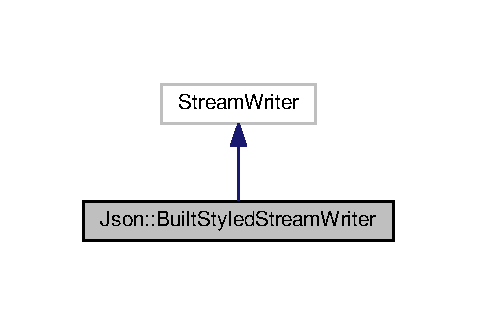
\includegraphics[width=229pt]{struct_json_1_1_built_styled_stream_writer__inherit__graph}
\end{center}
\end{figure}


Collaboration diagram for Json\+:\+:Built\+Styled\+Stream\+Writer\+:\nopagebreak
\begin{figure}[H]
\begin{center}
\leavevmode
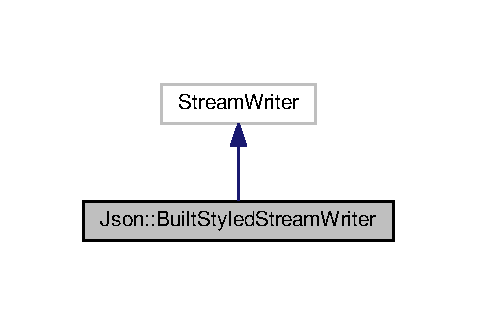
\includegraphics[width=229pt]{struct_json_1_1_built_styled_stream_writer__coll__graph}
\end{center}
\end{figure}
\subsection*{Public Member Functions}
\begin{DoxyCompactItemize}
\item 
\hyperlink{struct_json_1_1_built_styled_stream_writer_ab0c2e665c86b22f8fafb0e52c8069954}{Built\+Styled\+Stream\+Writer} (std\+::string const \&indentation, \hyperlink{struct_json_1_1_comment_style_a51fc08f3518fd81eba12f340d19a3d0c}{Comment\+Style\+::\+Enum} cs, std\+::string const \&colon\+Symbol, std\+::string const \&null\+Symbol, std\+::string const \&ending\+Line\+Feed\+Symbol, bool use\+Special\+Floats, unsigned int precision)
\item 
int \hyperlink{struct_json_1_1_built_styled_stream_writer_a2ecffc3d66c4feddf208e5cd3b1c0f18}{write} (Value const \&root, std\+::ostream $\ast$sout) override
\end{DoxyCompactItemize}
\subsection*{Private Types}
\begin{DoxyCompactItemize}
\item 
typedef std\+::vector$<$ std\+::string $>$ \hyperlink{struct_json_1_1_built_styled_stream_writer_a8356597862a354bcd55a7cb6e0512899}{Child\+Values}
\end{DoxyCompactItemize}
\subsection*{Private Member Functions}
\begin{DoxyCompactItemize}
\item 
void \hyperlink{struct_json_1_1_built_styled_stream_writer_a7c9da861861e570a51b45f270c9ff150}{write\+Value} (Value const \&value)
\item 
void \hyperlink{struct_json_1_1_built_styled_stream_writer_acd20e9274bbcf7876ef3af2e7d23a31f}{write\+Array\+Value} (Value const \&value)
\item 
bool \hyperlink{struct_json_1_1_built_styled_stream_writer_af423fd33b3d580506ea3efc53b05a077}{is\+Multine\+Array} (Value const \&value)
\item 
void \hyperlink{struct_json_1_1_built_styled_stream_writer_a53de0fe57c883d621c7255e49248651e}{push\+Value} (std\+::string const \&value)
\item 
void \hyperlink{struct_json_1_1_built_styled_stream_writer_a2b38a3714d415c4bd3b4812897130f3d}{write\+Indent} ()
\item 
void \hyperlink{struct_json_1_1_built_styled_stream_writer_a764c6d530b5bd660c4a7d1ad4eff6b8d}{write\+With\+Indent} (std\+::string const \&value)
\item 
void \hyperlink{struct_json_1_1_built_styled_stream_writer_a73e09692a2cfbd6e67836b060dc34a9f}{indent} ()
\item 
void \hyperlink{struct_json_1_1_built_styled_stream_writer_a0da6c6f603e00c8c6e38af553edd8c55}{unindent} ()
\item 
void \hyperlink{struct_json_1_1_built_styled_stream_writer_a32c4afca4e08fba79bb0a80a8010283a}{write\+Comment\+Before\+Value} (Value const \&root)
\item 
void \hyperlink{struct_json_1_1_built_styled_stream_writer_a89625b134fce0255263ca40e6125742b}{write\+Comment\+After\+Value\+On\+Same\+Line} (Value const \&root)
\end{DoxyCompactItemize}
\subsection*{Static Private Member Functions}
\begin{DoxyCompactItemize}
\item 
static bool \hyperlink{struct_json_1_1_built_styled_stream_writer_a457c2f3c1e8c952caeb60e52477d0c9a}{has\+Comment\+For\+Value} (const Value \&value)
\end{DoxyCompactItemize}
\subsection*{Private Attributes}
\begin{DoxyCompactItemize}
\item 
\hyperlink{struct_json_1_1_built_styled_stream_writer_a8356597862a354bcd55a7cb6e0512899}{Child\+Values} \hyperlink{struct_json_1_1_built_styled_stream_writer_a47d562d7874c5b1e68995bd62f575792}{child\+Values\+\_\+}
\item 
std\+::string \hyperlink{struct_json_1_1_built_styled_stream_writer_a2abfd5beb7f33adc3f690ce4f618aa2f}{indent\+String\+\_\+}
\item 
unsigned int \hyperlink{struct_json_1_1_built_styled_stream_writer_a06a51521ccae20397f52fe3036edc602}{right\+Margin\+\_\+}
\item 
std\+::string \hyperlink{struct_json_1_1_built_styled_stream_writer_ab1d7561ca0f480cb46cc113e1005e8ac}{indentation\+\_\+}
\item 
\hyperlink{struct_json_1_1_comment_style_a51fc08f3518fd81eba12f340d19a3d0c}{Comment\+Style\+::\+Enum} \hyperlink{struct_json_1_1_built_styled_stream_writer_a89a9c76c7531143b52785861ba21c1d4}{cs\+\_\+}
\item 
std\+::string \hyperlink{struct_json_1_1_built_styled_stream_writer_ac28b111b1c3ecc1ea6d981c8530ceca4}{colon\+Symbol\+\_\+}
\item 
std\+::string \hyperlink{struct_json_1_1_built_styled_stream_writer_a238a8f4737c9835af78ea80cc4f12658}{null\+Symbol\+\_\+}
\item 
std\+::string \hyperlink{struct_json_1_1_built_styled_stream_writer_a85a8c0e3c9deb2503d497f61bc0da74c}{ending\+Line\+Feed\+Symbol\+\_\+}
\item 
bool \hyperlink{struct_json_1_1_built_styled_stream_writer_abed9cc31da503b48798e7cea68c42e16}{add\+Child\+Values\+\_\+}\+: 1
\item 
bool \hyperlink{struct_json_1_1_built_styled_stream_writer_a6aa0ad023e623f600103631a6bca6d10}{indented\+\_\+}\+: 1
\item 
bool \hyperlink{struct_json_1_1_built_styled_stream_writer_a6f1b8694b4eb17ab8c34f6d6dd8c8a4a}{use\+Special\+Floats\+\_\+}\+: 1
\item 
unsigned int \hyperlink{struct_json_1_1_built_styled_stream_writer_a6373d8d0ae4741b64e3904e4db0eef46}{precision\+\_\+}
\end{DoxyCompactItemize}


\subsection{Detailed Description}


Definition at line 4810 of file jsoncpp.\+cpp.



\subsection{Member Typedef Documentation}
\index{Json\+::\+Built\+Styled\+Stream\+Writer@{Json\+::\+Built\+Styled\+Stream\+Writer}!Child\+Values@{Child\+Values}}
\index{Child\+Values@{Child\+Values}!Json\+::\+Built\+Styled\+Stream\+Writer@{Json\+::\+Built\+Styled\+Stream\+Writer}}
\subsubsection[{\texorpdfstring{Child\+Values}{ChildValues}}]{\setlength{\rightskip}{0pt plus 5cm}typedef std\+::vector$<$std\+::string$>$ {\bf Json\+::\+Built\+Styled\+Stream\+Writer\+::\+Child\+Values}\hspace{0.3cm}{\ttfamily [private]}}\hypertarget{struct_json_1_1_built_styled_stream_writer_a8356597862a354bcd55a7cb6e0512899}{}\label{struct_json_1_1_built_styled_stream_writer_a8356597862a354bcd55a7cb6e0512899}


Definition at line 4834 of file jsoncpp.\+cpp.



\subsection{Constructor \& Destructor Documentation}
\index{Json\+::\+Built\+Styled\+Stream\+Writer@{Json\+::\+Built\+Styled\+Stream\+Writer}!Built\+Styled\+Stream\+Writer@{Built\+Styled\+Stream\+Writer}}
\index{Built\+Styled\+Stream\+Writer@{Built\+Styled\+Stream\+Writer}!Json\+::\+Built\+Styled\+Stream\+Writer@{Json\+::\+Built\+Styled\+Stream\+Writer}}
\subsubsection[{\texorpdfstring{Built\+Styled\+Stream\+Writer(std\+::string const \&indentation, Comment\+Style\+::\+Enum cs, std\+::string const \&colon\+Symbol, std\+::string const \&null\+Symbol, std\+::string const \&ending\+Line\+Feed\+Symbol, bool use\+Special\+Floats, unsigned int precision)}{BuiltStyledStreamWriter(std::string const &indentation, CommentStyle::Enum cs, std::string const &colonSymbol, std::string const &nullSymbol, std::string const &endingLineFeedSymbol, bool useSpecialFloats, unsigned int precision)}}]{\setlength{\rightskip}{0pt plus 5cm}Json\+::\+Built\+Styled\+Stream\+Writer\+::\+Built\+Styled\+Stream\+Writer (
\begin{DoxyParamCaption}
\item[{std\+::string const \&}]{indentation, }
\item[{{\bf Comment\+Style\+::\+Enum}}]{cs, }
\item[{std\+::string const \&}]{colon\+Symbol, }
\item[{std\+::string const \&}]{null\+Symbol, }
\item[{std\+::string const \&}]{ending\+Line\+Feed\+Symbol, }
\item[{bool}]{use\+Special\+Floats, }
\item[{unsigned int}]{precision}
\end{DoxyParamCaption}
)}\hypertarget{struct_json_1_1_built_styled_stream_writer_ab0c2e665c86b22f8fafb0e52c8069954}{}\label{struct_json_1_1_built_styled_stream_writer_ab0c2e665c86b22f8fafb0e52c8069954}


Definition at line 4849 of file jsoncpp.\+cpp.



Here is the caller graph for this function\+:\nopagebreak
\begin{figure}[H]
\begin{center}
\leavevmode
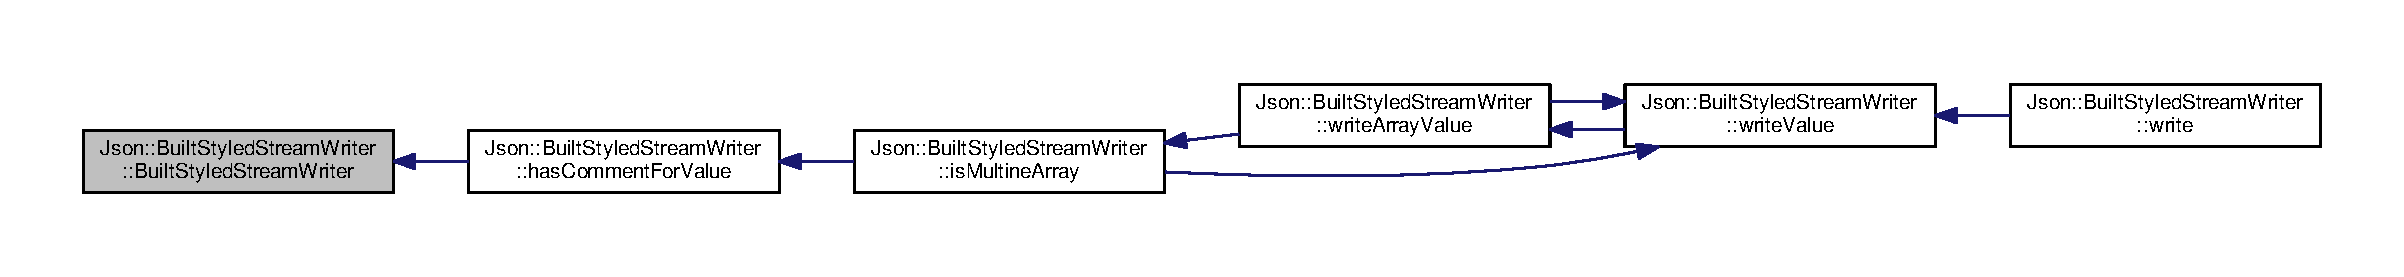
\includegraphics[width=350pt]{struct_json_1_1_built_styled_stream_writer_ab0c2e665c86b22f8fafb0e52c8069954_icgraph}
\end{center}
\end{figure}




\subsection{Member Function Documentation}
\index{Json\+::\+Built\+Styled\+Stream\+Writer@{Json\+::\+Built\+Styled\+Stream\+Writer}!has\+Comment\+For\+Value@{has\+Comment\+For\+Value}}
\index{has\+Comment\+For\+Value@{has\+Comment\+For\+Value}!Json\+::\+Built\+Styled\+Stream\+Writer@{Json\+::\+Built\+Styled\+Stream\+Writer}}
\subsubsection[{\texorpdfstring{has\+Comment\+For\+Value(const Value \&value)}{hasCommentForValue(const Value &value)}}]{\setlength{\rightskip}{0pt plus 5cm}bool Json\+::\+Built\+Styled\+Stream\+Writer\+::has\+Comment\+For\+Value (
\begin{DoxyParamCaption}
\item[{const Value \&}]{value}
\end{DoxyParamCaption}
)\hspace{0.3cm}{\ttfamily [static]}, {\ttfamily [private]}}\hypertarget{struct_json_1_1_built_styled_stream_writer_a457c2f3c1e8c952caeb60e52477d0c9a}{}\label{struct_json_1_1_built_styled_stream_writer_a457c2f3c1e8c952caeb60e52477d0c9a}


Definition at line 5080 of file jsoncpp.\+cpp.



Here is the call graph for this function\+:\nopagebreak
\begin{figure}[H]
\begin{center}
\leavevmode
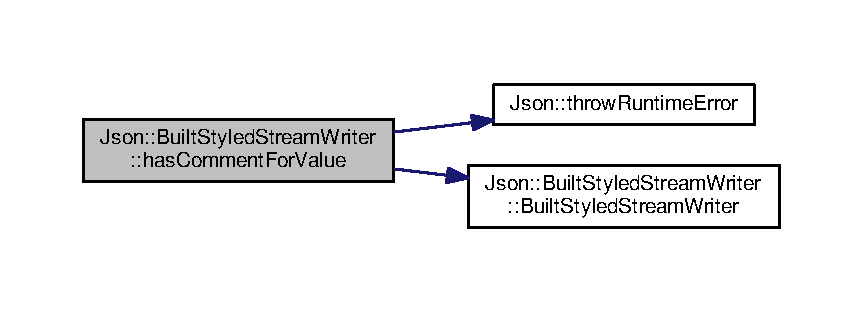
\includegraphics[width=350pt]{struct_json_1_1_built_styled_stream_writer_a457c2f3c1e8c952caeb60e52477d0c9a_cgraph}
\end{center}
\end{figure}




Here is the caller graph for this function\+:\nopagebreak
\begin{figure}[H]
\begin{center}
\leavevmode
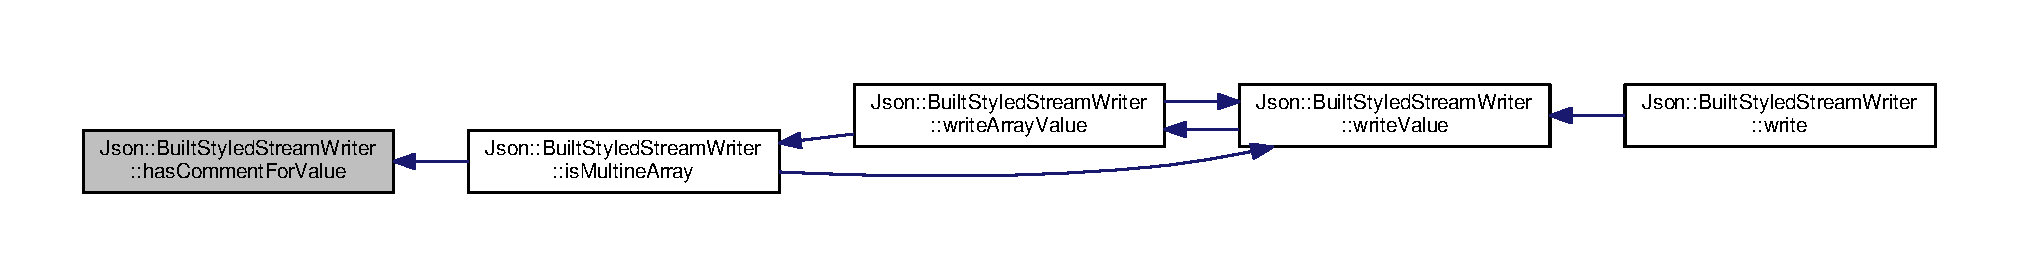
\includegraphics[width=350pt]{struct_json_1_1_built_styled_stream_writer_a457c2f3c1e8c952caeb60e52477d0c9a_icgraph}
\end{center}
\end{figure}


\index{Json\+::\+Built\+Styled\+Stream\+Writer@{Json\+::\+Built\+Styled\+Stream\+Writer}!indent@{indent}}
\index{indent@{indent}!Json\+::\+Built\+Styled\+Stream\+Writer@{Json\+::\+Built\+Styled\+Stream\+Writer}}
\subsubsection[{\texorpdfstring{indent()}{indent()}}]{\setlength{\rightskip}{0pt plus 5cm}void Json\+::\+Built\+Styled\+Stream\+Writer\+::indent (
\begin{DoxyParamCaption}
{}
\end{DoxyParamCaption}
)\hspace{0.3cm}{\ttfamily [private]}}\hypertarget{struct_json_1_1_built_styled_stream_writer_a73e09692a2cfbd6e67836b060dc34a9f}{}\label{struct_json_1_1_built_styled_stream_writer_a73e09692a2cfbd6e67836b060dc34a9f}


Definition at line 5042 of file jsoncpp.\+cpp.



Here is the caller graph for this function\+:\nopagebreak
\begin{figure}[H]
\begin{center}
\leavevmode
\includegraphics[width=350pt]{struct_json_1_1_built_styled_stream_writer_a73e09692a2cfbd6e67836b060dc34a9f_icgraph}
\end{center}
\end{figure}


\index{Json\+::\+Built\+Styled\+Stream\+Writer@{Json\+::\+Built\+Styled\+Stream\+Writer}!is\+Multine\+Array@{is\+Multine\+Array}}
\index{is\+Multine\+Array@{is\+Multine\+Array}!Json\+::\+Built\+Styled\+Stream\+Writer@{Json\+::\+Built\+Styled\+Stream\+Writer}}
\subsubsection[{\texorpdfstring{is\+Multine\+Array(\+Value const \&value)}{isMultineArray(Value const &value)}}]{\setlength{\rightskip}{0pt plus 5cm}bool Json\+::\+Built\+Styled\+Stream\+Writer\+::is\+Multine\+Array (
\begin{DoxyParamCaption}
\item[{Value const \&}]{value}
\end{DoxyParamCaption}
)\hspace{0.3cm}{\ttfamily [private]}}\hypertarget{struct_json_1_1_built_styled_stream_writer_af423fd33b3d580506ea3efc53b05a077}{}\label{struct_json_1_1_built_styled_stream_writer_af423fd33b3d580506ea3efc53b05a077}


Definition at line 4990 of file jsoncpp.\+cpp.



Here is the call graph for this function\+:\nopagebreak
\begin{figure}[H]
\begin{center}
\leavevmode
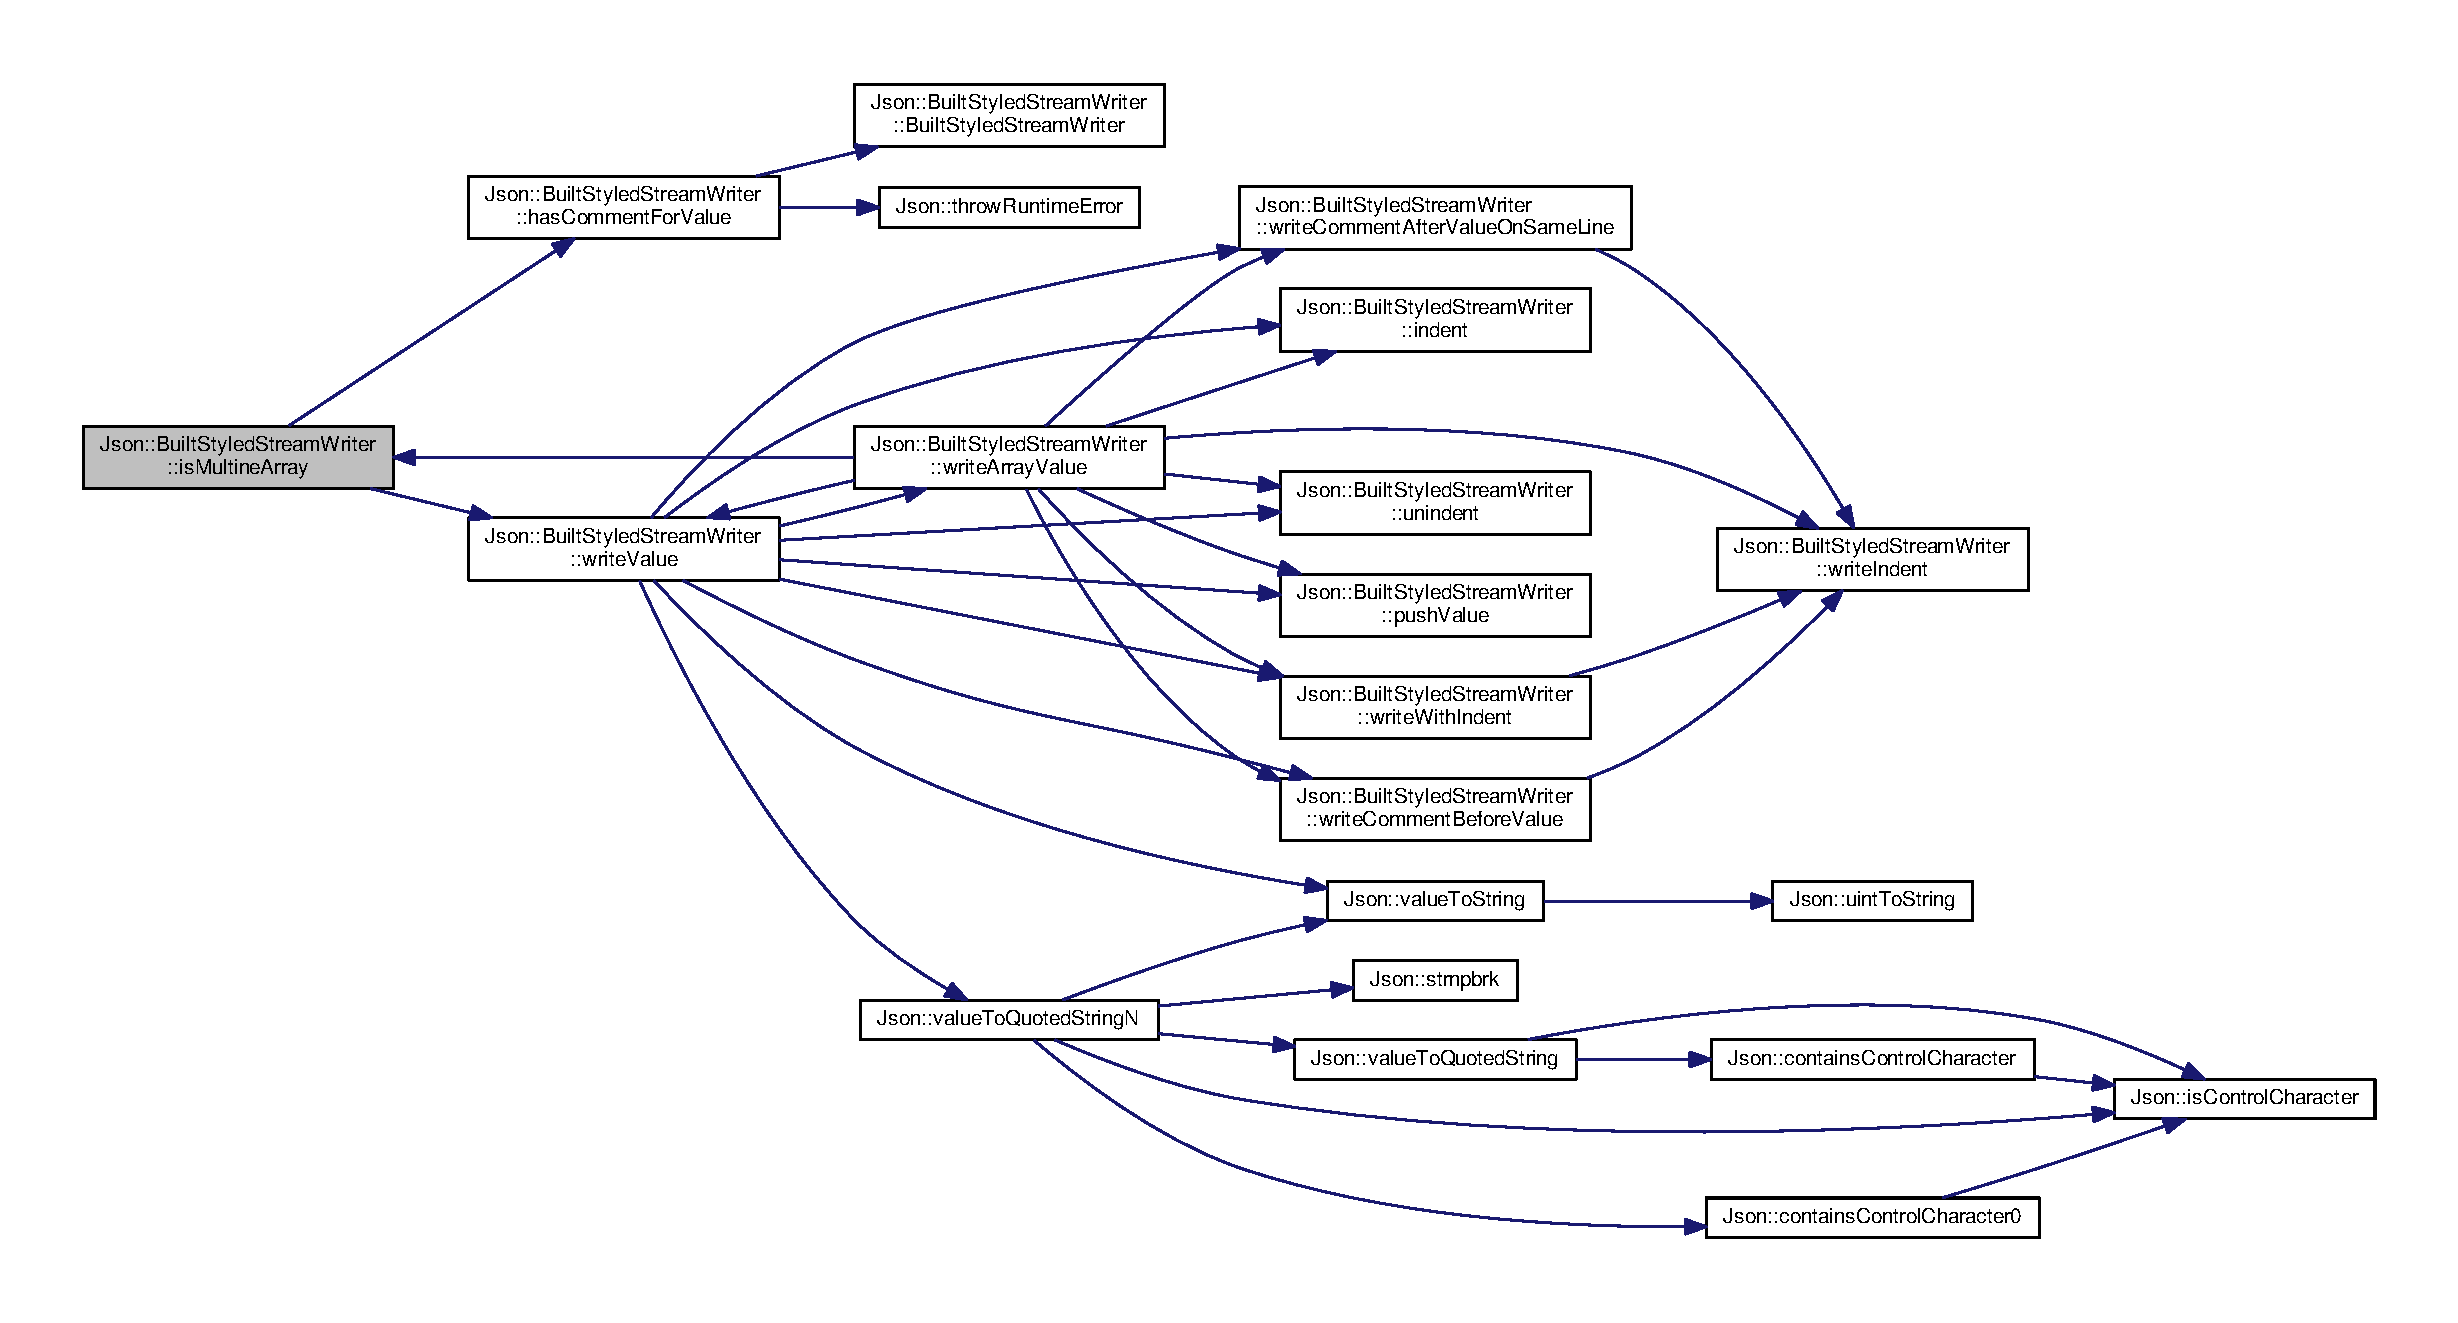
\includegraphics[width=350pt]{struct_json_1_1_built_styled_stream_writer_af423fd33b3d580506ea3efc53b05a077_cgraph}
\end{center}
\end{figure}




Here is the caller graph for this function\+:\nopagebreak
\begin{figure}[H]
\begin{center}
\leavevmode
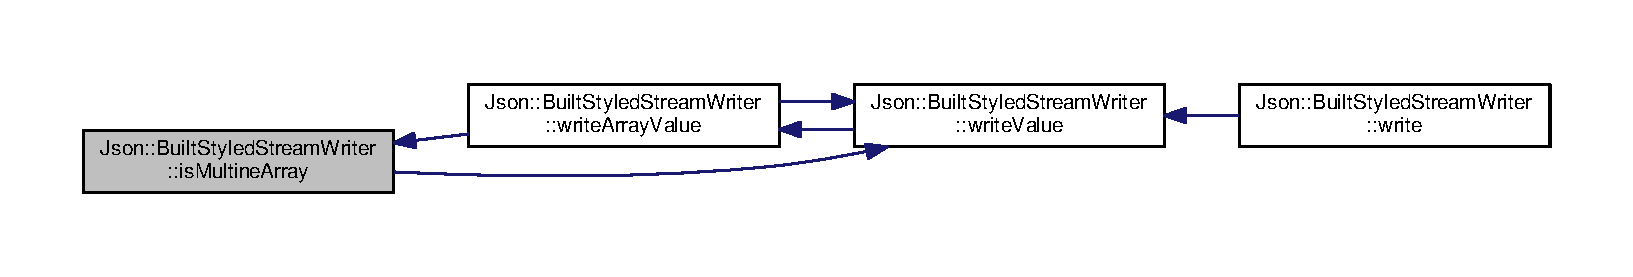
\includegraphics[width=350pt]{struct_json_1_1_built_styled_stream_writer_af423fd33b3d580506ea3efc53b05a077_icgraph}
\end{center}
\end{figure}


\index{Json\+::\+Built\+Styled\+Stream\+Writer@{Json\+::\+Built\+Styled\+Stream\+Writer}!push\+Value@{push\+Value}}
\index{push\+Value@{push\+Value}!Json\+::\+Built\+Styled\+Stream\+Writer@{Json\+::\+Built\+Styled\+Stream\+Writer}}
\subsubsection[{\texorpdfstring{push\+Value(std\+::string const \&value)}{pushValue(std::string const &value)}}]{\setlength{\rightskip}{0pt plus 5cm}void Json\+::\+Built\+Styled\+Stream\+Writer\+::push\+Value (
\begin{DoxyParamCaption}
\item[{std\+::string const \&}]{value}
\end{DoxyParamCaption}
)\hspace{0.3cm}{\ttfamily [private]}}\hypertarget{struct_json_1_1_built_styled_stream_writer_a53de0fe57c883d621c7255e49248651e}{}\label{struct_json_1_1_built_styled_stream_writer_a53de0fe57c883d621c7255e49248651e}


Definition at line 5017 of file jsoncpp.\+cpp.



Here is the caller graph for this function\+:\nopagebreak
\begin{figure}[H]
\begin{center}
\leavevmode
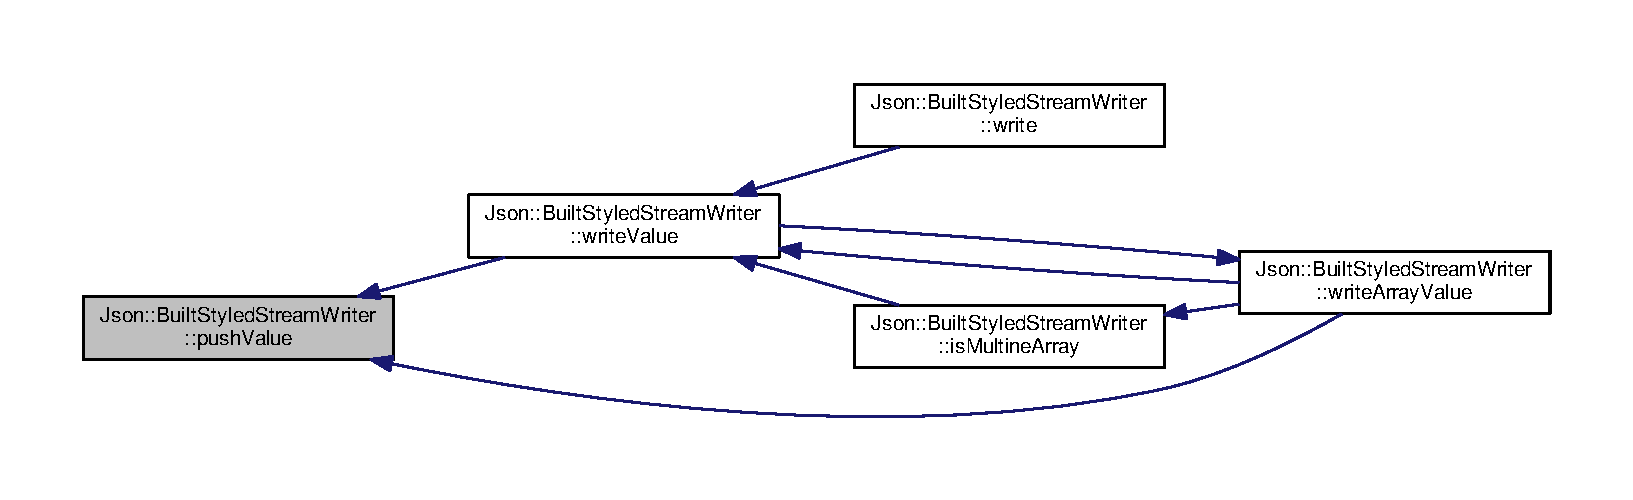
\includegraphics[width=350pt]{struct_json_1_1_built_styled_stream_writer_a53de0fe57c883d621c7255e49248651e_icgraph}
\end{center}
\end{figure}


\index{Json\+::\+Built\+Styled\+Stream\+Writer@{Json\+::\+Built\+Styled\+Stream\+Writer}!unindent@{unindent}}
\index{unindent@{unindent}!Json\+::\+Built\+Styled\+Stream\+Writer@{Json\+::\+Built\+Styled\+Stream\+Writer}}
\subsubsection[{\texorpdfstring{unindent()}{unindent()}}]{\setlength{\rightskip}{0pt plus 5cm}void Json\+::\+Built\+Styled\+Stream\+Writer\+::unindent (
\begin{DoxyParamCaption}
{}
\end{DoxyParamCaption}
)\hspace{0.3cm}{\ttfamily [private]}}\hypertarget{struct_json_1_1_built_styled_stream_writer_a0da6c6f603e00c8c6e38af553edd8c55}{}\label{struct_json_1_1_built_styled_stream_writer_a0da6c6f603e00c8c6e38af553edd8c55}


Definition at line 5044 of file jsoncpp.\+cpp.



Here is the caller graph for this function\+:\nopagebreak
\begin{figure}[H]
\begin{center}
\leavevmode
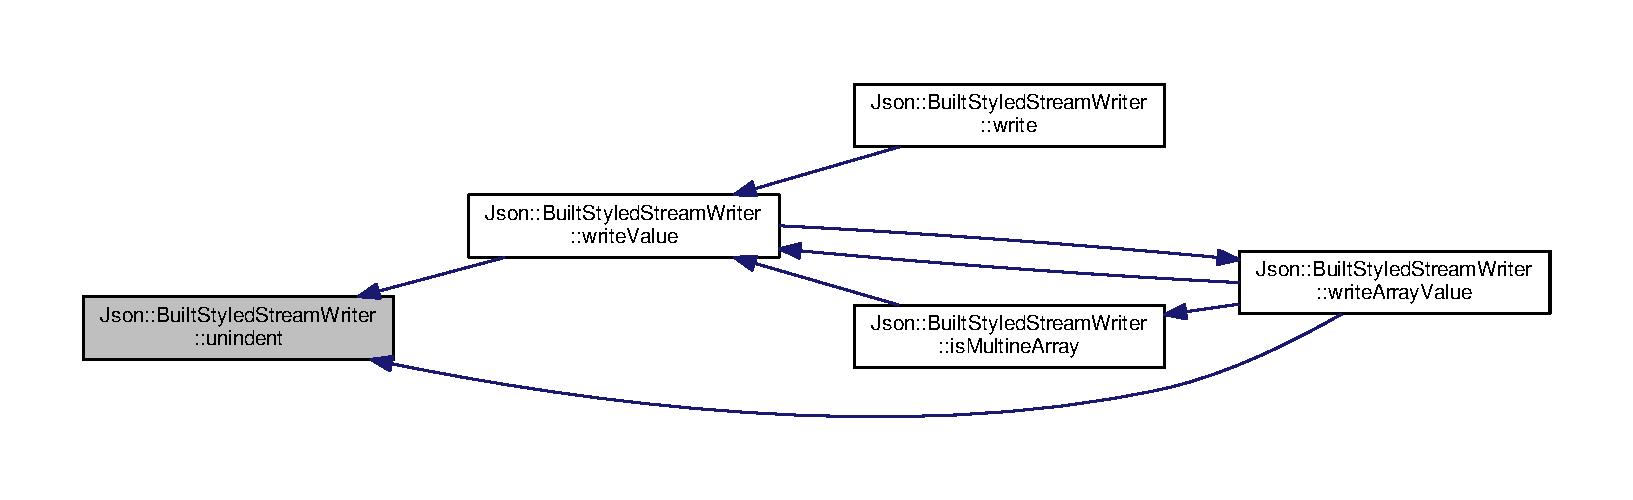
\includegraphics[width=350pt]{struct_json_1_1_built_styled_stream_writer_a0da6c6f603e00c8c6e38af553edd8c55_icgraph}
\end{center}
\end{figure}


\index{Json\+::\+Built\+Styled\+Stream\+Writer@{Json\+::\+Built\+Styled\+Stream\+Writer}!write@{write}}
\index{write@{write}!Json\+::\+Built\+Styled\+Stream\+Writer@{Json\+::\+Built\+Styled\+Stream\+Writer}}
\subsubsection[{\texorpdfstring{write(\+Value const \&root, std\+::ostream $\ast$sout) override}{write(Value const &root, std::ostream *sout) override}}]{\setlength{\rightskip}{0pt plus 5cm}int Json\+::\+Built\+Styled\+Stream\+Writer\+::write (
\begin{DoxyParamCaption}
\item[{Value const \&}]{root, }
\item[{std\+::ostream $\ast$}]{sout}
\end{DoxyParamCaption}
)\hspace{0.3cm}{\ttfamily [override]}}\hypertarget{struct_json_1_1_built_styled_stream_writer_a2ecffc3d66c4feddf208e5cd3b1c0f18}{}\label{struct_json_1_1_built_styled_stream_writer_a2ecffc3d66c4feddf208e5cd3b1c0f18}


Definition at line 4869 of file jsoncpp.\+cpp.



Here is the call graph for this function\+:\nopagebreak
\begin{figure}[H]
\begin{center}
\leavevmode
\includegraphics[width=350pt]{struct_json_1_1_built_styled_stream_writer_a2ecffc3d66c4feddf208e5cd3b1c0f18_cgraph}
\end{center}
\end{figure}


\index{Json\+::\+Built\+Styled\+Stream\+Writer@{Json\+::\+Built\+Styled\+Stream\+Writer}!write\+Array\+Value@{write\+Array\+Value}}
\index{write\+Array\+Value@{write\+Array\+Value}!Json\+::\+Built\+Styled\+Stream\+Writer@{Json\+::\+Built\+Styled\+Stream\+Writer}}
\subsubsection[{\texorpdfstring{write\+Array\+Value(\+Value const \&value)}{writeArrayValue(Value const &value)}}]{\setlength{\rightskip}{0pt plus 5cm}void Json\+::\+Built\+Styled\+Stream\+Writer\+::write\+Array\+Value (
\begin{DoxyParamCaption}
\item[{Value const \&}]{value}
\end{DoxyParamCaption}
)\hspace{0.3cm}{\ttfamily [private]}}\hypertarget{struct_json_1_1_built_styled_stream_writer_acd20e9274bbcf7876ef3af2e7d23a31f}{}\label{struct_json_1_1_built_styled_stream_writer_acd20e9274bbcf7876ef3af2e7d23a31f}


Definition at line 4943 of file jsoncpp.\+cpp.



Here is the call graph for this function\+:\nopagebreak
\begin{figure}[H]
\begin{center}
\leavevmode
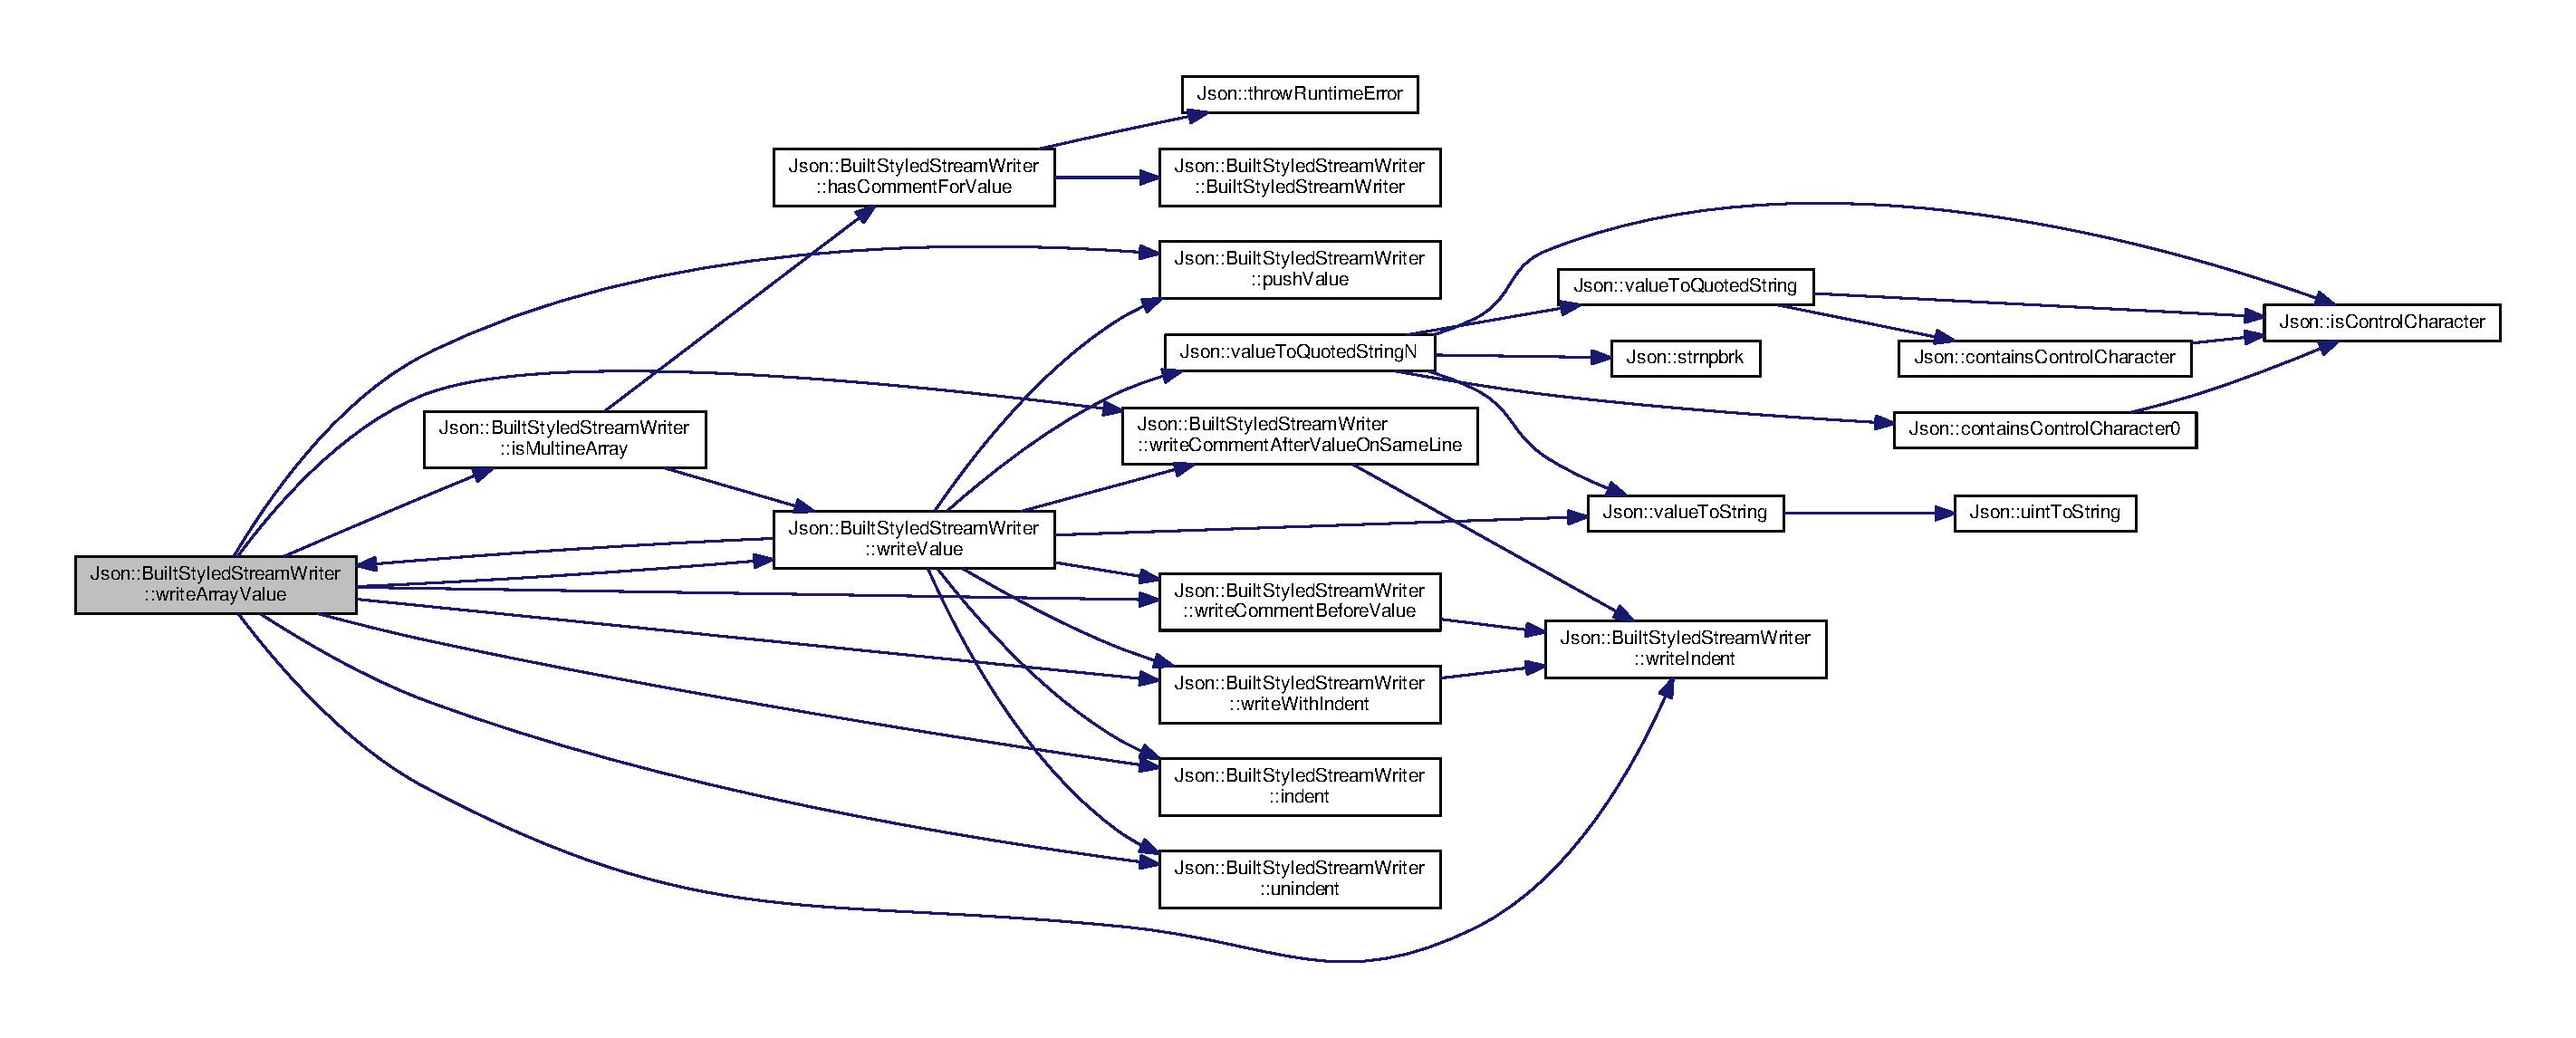
\includegraphics[width=350pt]{struct_json_1_1_built_styled_stream_writer_acd20e9274bbcf7876ef3af2e7d23a31f_cgraph}
\end{center}
\end{figure}




Here is the caller graph for this function\+:\nopagebreak
\begin{figure}[H]
\begin{center}
\leavevmode
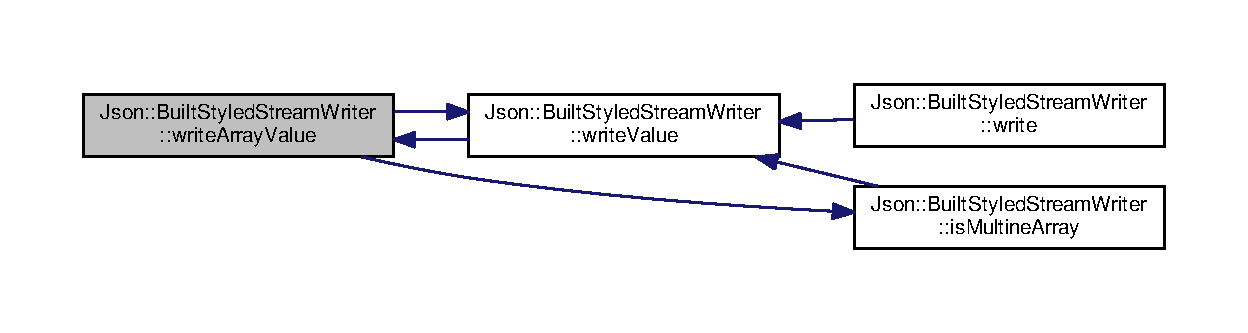
\includegraphics[width=350pt]{struct_json_1_1_built_styled_stream_writer_acd20e9274bbcf7876ef3af2e7d23a31f_icgraph}
\end{center}
\end{figure}


\index{Json\+::\+Built\+Styled\+Stream\+Writer@{Json\+::\+Built\+Styled\+Stream\+Writer}!write\+Comment\+After\+Value\+On\+Same\+Line@{write\+Comment\+After\+Value\+On\+Same\+Line}}
\index{write\+Comment\+After\+Value\+On\+Same\+Line@{write\+Comment\+After\+Value\+On\+Same\+Line}!Json\+::\+Built\+Styled\+Stream\+Writer@{Json\+::\+Built\+Styled\+Stream\+Writer}}
\subsubsection[{\texorpdfstring{write\+Comment\+After\+Value\+On\+Same\+Line(\+Value const \&root)}{writeCommentAfterValueOnSameLine(Value const &root)}}]{\setlength{\rightskip}{0pt plus 5cm}void Json\+::\+Built\+Styled\+Stream\+Writer\+::write\+Comment\+After\+Value\+On\+Same\+Line (
\begin{DoxyParamCaption}
\item[{Value const \&}]{root}
\end{DoxyParamCaption}
)\hspace{0.3cm}{\ttfamily [private]}}\hypertarget{struct_json_1_1_built_styled_stream_writer_a89625b134fce0255263ca40e6125742b}{}\label{struct_json_1_1_built_styled_stream_writer_a89625b134fce0255263ca40e6125742b}


Definition at line 5068 of file jsoncpp.\+cpp.



Here is the call graph for this function\+:\nopagebreak
\begin{figure}[H]
\begin{center}
\leavevmode
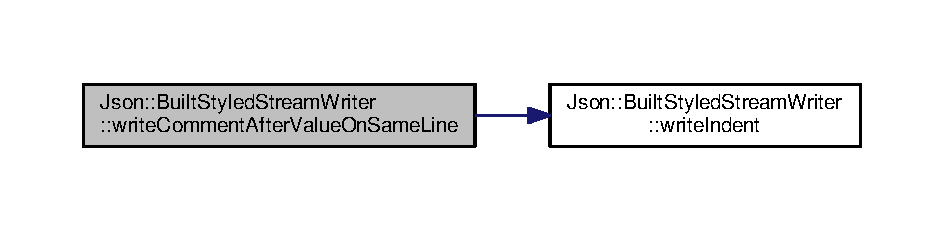
\includegraphics[width=350pt]{struct_json_1_1_built_styled_stream_writer_a89625b134fce0255263ca40e6125742b_cgraph}
\end{center}
\end{figure}




Here is the caller graph for this function\+:\nopagebreak
\begin{figure}[H]
\begin{center}
\leavevmode
\includegraphics[width=350pt]{struct_json_1_1_built_styled_stream_writer_a89625b134fce0255263ca40e6125742b_icgraph}
\end{center}
\end{figure}


\index{Json\+::\+Built\+Styled\+Stream\+Writer@{Json\+::\+Built\+Styled\+Stream\+Writer}!write\+Comment\+Before\+Value@{write\+Comment\+Before\+Value}}
\index{write\+Comment\+Before\+Value@{write\+Comment\+Before\+Value}!Json\+::\+Built\+Styled\+Stream\+Writer@{Json\+::\+Built\+Styled\+Stream\+Writer}}
\subsubsection[{\texorpdfstring{write\+Comment\+Before\+Value(\+Value const \&root)}{writeCommentBeforeValue(Value const &root)}}]{\setlength{\rightskip}{0pt plus 5cm}void Json\+::\+Built\+Styled\+Stream\+Writer\+::write\+Comment\+Before\+Value (
\begin{DoxyParamCaption}
\item[{Value const \&}]{root}
\end{DoxyParamCaption}
)\hspace{0.3cm}{\ttfamily [private]}}\hypertarget{struct_json_1_1_built_styled_stream_writer_a32c4afca4e08fba79bb0a80a8010283a}{}\label{struct_json_1_1_built_styled_stream_writer_a32c4afca4e08fba79bb0a80a8010283a}


Definition at line 5049 of file jsoncpp.\+cpp.



Here is the call graph for this function\+:\nopagebreak
\begin{figure}[H]
\begin{center}
\leavevmode
\includegraphics[width=350pt]{struct_json_1_1_built_styled_stream_writer_a32c4afca4e08fba79bb0a80a8010283a_cgraph}
\end{center}
\end{figure}




Here is the caller graph for this function\+:\nopagebreak
\begin{figure}[H]
\begin{center}
\leavevmode
\includegraphics[width=350pt]{struct_json_1_1_built_styled_stream_writer_a32c4afca4e08fba79bb0a80a8010283a_icgraph}
\end{center}
\end{figure}


\index{Json\+::\+Built\+Styled\+Stream\+Writer@{Json\+::\+Built\+Styled\+Stream\+Writer}!write\+Indent@{write\+Indent}}
\index{write\+Indent@{write\+Indent}!Json\+::\+Built\+Styled\+Stream\+Writer@{Json\+::\+Built\+Styled\+Stream\+Writer}}
\subsubsection[{\texorpdfstring{write\+Indent()}{writeIndent()}}]{\setlength{\rightskip}{0pt plus 5cm}void Json\+::\+Built\+Styled\+Stream\+Writer\+::write\+Indent (
\begin{DoxyParamCaption}
{}
\end{DoxyParamCaption}
)\hspace{0.3cm}{\ttfamily [private]}}\hypertarget{struct_json_1_1_built_styled_stream_writer_a2b38a3714d415c4bd3b4812897130f3d}{}\label{struct_json_1_1_built_styled_stream_writer_a2b38a3714d415c4bd3b4812897130f3d}


Definition at line 5024 of file jsoncpp.\+cpp.



Here is the caller graph for this function\+:\nopagebreak
\begin{figure}[H]
\begin{center}
\leavevmode
\includegraphics[width=350pt]{struct_json_1_1_built_styled_stream_writer_a2b38a3714d415c4bd3b4812897130f3d_icgraph}
\end{center}
\end{figure}


\index{Json\+::\+Built\+Styled\+Stream\+Writer@{Json\+::\+Built\+Styled\+Stream\+Writer}!write\+Value@{write\+Value}}
\index{write\+Value@{write\+Value}!Json\+::\+Built\+Styled\+Stream\+Writer@{Json\+::\+Built\+Styled\+Stream\+Writer}}
\subsubsection[{\texorpdfstring{write\+Value(\+Value const \&value)}{writeValue(Value const &value)}}]{\setlength{\rightskip}{0pt plus 5cm}void Json\+::\+Built\+Styled\+Stream\+Writer\+::write\+Value (
\begin{DoxyParamCaption}
\item[{Value const \&}]{value}
\end{DoxyParamCaption}
)\hspace{0.3cm}{\ttfamily [private]}}\hypertarget{struct_json_1_1_built_styled_stream_writer_a7c9da861861e570a51b45f270c9ff150}{}\label{struct_json_1_1_built_styled_stream_writer_a7c9da861861e570a51b45f270c9ff150}


Definition at line 4884 of file jsoncpp.\+cpp.



Here is the call graph for this function\+:\nopagebreak
\begin{figure}[H]
\begin{center}
\leavevmode
\includegraphics[width=350pt]{struct_json_1_1_built_styled_stream_writer_a7c9da861861e570a51b45f270c9ff150_cgraph}
\end{center}
\end{figure}




Here is the caller graph for this function\+:\nopagebreak
\begin{figure}[H]
\begin{center}
\leavevmode
\includegraphics[width=350pt]{struct_json_1_1_built_styled_stream_writer_a7c9da861861e570a51b45f270c9ff150_icgraph}
\end{center}
\end{figure}


\index{Json\+::\+Built\+Styled\+Stream\+Writer@{Json\+::\+Built\+Styled\+Stream\+Writer}!write\+With\+Indent@{write\+With\+Indent}}
\index{write\+With\+Indent@{write\+With\+Indent}!Json\+::\+Built\+Styled\+Stream\+Writer@{Json\+::\+Built\+Styled\+Stream\+Writer}}
\subsubsection[{\texorpdfstring{write\+With\+Indent(std\+::string const \&value)}{writeWithIndent(std::string const &value)}}]{\setlength{\rightskip}{0pt plus 5cm}void Json\+::\+Built\+Styled\+Stream\+Writer\+::write\+With\+Indent (
\begin{DoxyParamCaption}
\item[{std\+::string const \&}]{value}
\end{DoxyParamCaption}
)\hspace{0.3cm}{\ttfamily [private]}}\hypertarget{struct_json_1_1_built_styled_stream_writer_a764c6d530b5bd660c4a7d1ad4eff6b8d}{}\label{struct_json_1_1_built_styled_stream_writer_a764c6d530b5bd660c4a7d1ad4eff6b8d}


Definition at line 5036 of file jsoncpp.\+cpp.



Here is the call graph for this function\+:\nopagebreak
\begin{figure}[H]
\begin{center}
\leavevmode
\includegraphics[width=350pt]{struct_json_1_1_built_styled_stream_writer_a764c6d530b5bd660c4a7d1ad4eff6b8d_cgraph}
\end{center}
\end{figure}




Here is the caller graph for this function\+:\nopagebreak
\begin{figure}[H]
\begin{center}
\leavevmode
\includegraphics[width=350pt]{struct_json_1_1_built_styled_stream_writer_a764c6d530b5bd660c4a7d1ad4eff6b8d_icgraph}
\end{center}
\end{figure}




\subsection{Member Data Documentation}
\index{Json\+::\+Built\+Styled\+Stream\+Writer@{Json\+::\+Built\+Styled\+Stream\+Writer}!add\+Child\+Values\+\_\+@{add\+Child\+Values\+\_\+}}
\index{add\+Child\+Values\+\_\+@{add\+Child\+Values\+\_\+}!Json\+::\+Built\+Styled\+Stream\+Writer@{Json\+::\+Built\+Styled\+Stream\+Writer}}
\subsubsection[{\texorpdfstring{add\+Child\+Values\+\_\+}{addChildValues_}}]{\setlength{\rightskip}{0pt plus 5cm}bool Json\+::\+Built\+Styled\+Stream\+Writer\+::add\+Child\+Values\+\_\+\hspace{0.3cm}{\ttfamily [private]}}\hypertarget{struct_json_1_1_built_styled_stream_writer_abed9cc31da503b48798e7cea68c42e16}{}\label{struct_json_1_1_built_styled_stream_writer_abed9cc31da503b48798e7cea68c42e16}


Definition at line 4844 of file jsoncpp.\+cpp.

\index{Json\+::\+Built\+Styled\+Stream\+Writer@{Json\+::\+Built\+Styled\+Stream\+Writer}!child\+Values\+\_\+@{child\+Values\+\_\+}}
\index{child\+Values\+\_\+@{child\+Values\+\_\+}!Json\+::\+Built\+Styled\+Stream\+Writer@{Json\+::\+Built\+Styled\+Stream\+Writer}}
\subsubsection[{\texorpdfstring{child\+Values\+\_\+}{childValues_}}]{\setlength{\rightskip}{0pt plus 5cm}{\bf Child\+Values} Json\+::\+Built\+Styled\+Stream\+Writer\+::child\+Values\+\_\+\hspace{0.3cm}{\ttfamily [private]}}\hypertarget{struct_json_1_1_built_styled_stream_writer_a47d562d7874c5b1e68995bd62f575792}{}\label{struct_json_1_1_built_styled_stream_writer_a47d562d7874c5b1e68995bd62f575792}


Definition at line 4836 of file jsoncpp.\+cpp.

\index{Json\+::\+Built\+Styled\+Stream\+Writer@{Json\+::\+Built\+Styled\+Stream\+Writer}!colon\+Symbol\+\_\+@{colon\+Symbol\+\_\+}}
\index{colon\+Symbol\+\_\+@{colon\+Symbol\+\_\+}!Json\+::\+Built\+Styled\+Stream\+Writer@{Json\+::\+Built\+Styled\+Stream\+Writer}}
\subsubsection[{\texorpdfstring{colon\+Symbol\+\_\+}{colonSymbol_}}]{\setlength{\rightskip}{0pt plus 5cm}std\+::string Json\+::\+Built\+Styled\+Stream\+Writer\+::colon\+Symbol\+\_\+\hspace{0.3cm}{\ttfamily [private]}}\hypertarget{struct_json_1_1_built_styled_stream_writer_ac28b111b1c3ecc1ea6d981c8530ceca4}{}\label{struct_json_1_1_built_styled_stream_writer_ac28b111b1c3ecc1ea6d981c8530ceca4}


Definition at line 4841 of file jsoncpp.\+cpp.

\index{Json\+::\+Built\+Styled\+Stream\+Writer@{Json\+::\+Built\+Styled\+Stream\+Writer}!cs\+\_\+@{cs\+\_\+}}
\index{cs\+\_\+@{cs\+\_\+}!Json\+::\+Built\+Styled\+Stream\+Writer@{Json\+::\+Built\+Styled\+Stream\+Writer}}
\subsubsection[{\texorpdfstring{cs\+\_\+}{cs_}}]{\setlength{\rightskip}{0pt plus 5cm}{\bf Comment\+Style\+::\+Enum} Json\+::\+Built\+Styled\+Stream\+Writer\+::cs\+\_\+\hspace{0.3cm}{\ttfamily [private]}}\hypertarget{struct_json_1_1_built_styled_stream_writer_a89a9c76c7531143b52785861ba21c1d4}{}\label{struct_json_1_1_built_styled_stream_writer_a89a9c76c7531143b52785861ba21c1d4}


Definition at line 4840 of file jsoncpp.\+cpp.

\index{Json\+::\+Built\+Styled\+Stream\+Writer@{Json\+::\+Built\+Styled\+Stream\+Writer}!ending\+Line\+Feed\+Symbol\+\_\+@{ending\+Line\+Feed\+Symbol\+\_\+}}
\index{ending\+Line\+Feed\+Symbol\+\_\+@{ending\+Line\+Feed\+Symbol\+\_\+}!Json\+::\+Built\+Styled\+Stream\+Writer@{Json\+::\+Built\+Styled\+Stream\+Writer}}
\subsubsection[{\texorpdfstring{ending\+Line\+Feed\+Symbol\+\_\+}{endingLineFeedSymbol_}}]{\setlength{\rightskip}{0pt plus 5cm}std\+::string Json\+::\+Built\+Styled\+Stream\+Writer\+::ending\+Line\+Feed\+Symbol\+\_\+\hspace{0.3cm}{\ttfamily [private]}}\hypertarget{struct_json_1_1_built_styled_stream_writer_a85a8c0e3c9deb2503d497f61bc0da74c}{}\label{struct_json_1_1_built_styled_stream_writer_a85a8c0e3c9deb2503d497f61bc0da74c}


Definition at line 4843 of file jsoncpp.\+cpp.

\index{Json\+::\+Built\+Styled\+Stream\+Writer@{Json\+::\+Built\+Styled\+Stream\+Writer}!indentation\+\_\+@{indentation\+\_\+}}
\index{indentation\+\_\+@{indentation\+\_\+}!Json\+::\+Built\+Styled\+Stream\+Writer@{Json\+::\+Built\+Styled\+Stream\+Writer}}
\subsubsection[{\texorpdfstring{indentation\+\_\+}{indentation_}}]{\setlength{\rightskip}{0pt plus 5cm}std\+::string Json\+::\+Built\+Styled\+Stream\+Writer\+::indentation\+\_\+\hspace{0.3cm}{\ttfamily [private]}}\hypertarget{struct_json_1_1_built_styled_stream_writer_ab1d7561ca0f480cb46cc113e1005e8ac}{}\label{struct_json_1_1_built_styled_stream_writer_ab1d7561ca0f480cb46cc113e1005e8ac}


Definition at line 4839 of file jsoncpp.\+cpp.

\index{Json\+::\+Built\+Styled\+Stream\+Writer@{Json\+::\+Built\+Styled\+Stream\+Writer}!indented\+\_\+@{indented\+\_\+}}
\index{indented\+\_\+@{indented\+\_\+}!Json\+::\+Built\+Styled\+Stream\+Writer@{Json\+::\+Built\+Styled\+Stream\+Writer}}
\subsubsection[{\texorpdfstring{indented\+\_\+}{indented_}}]{\setlength{\rightskip}{0pt plus 5cm}bool Json\+::\+Built\+Styled\+Stream\+Writer\+::indented\+\_\+\hspace{0.3cm}{\ttfamily [private]}}\hypertarget{struct_json_1_1_built_styled_stream_writer_a6aa0ad023e623f600103631a6bca6d10}{}\label{struct_json_1_1_built_styled_stream_writer_a6aa0ad023e623f600103631a6bca6d10}


Definition at line 4845 of file jsoncpp.\+cpp.

\index{Json\+::\+Built\+Styled\+Stream\+Writer@{Json\+::\+Built\+Styled\+Stream\+Writer}!indent\+String\+\_\+@{indent\+String\+\_\+}}
\index{indent\+String\+\_\+@{indent\+String\+\_\+}!Json\+::\+Built\+Styled\+Stream\+Writer@{Json\+::\+Built\+Styled\+Stream\+Writer}}
\subsubsection[{\texorpdfstring{indent\+String\+\_\+}{indentString_}}]{\setlength{\rightskip}{0pt plus 5cm}std\+::string Json\+::\+Built\+Styled\+Stream\+Writer\+::indent\+String\+\_\+\hspace{0.3cm}{\ttfamily [private]}}\hypertarget{struct_json_1_1_built_styled_stream_writer_a2abfd5beb7f33adc3f690ce4f618aa2f}{}\label{struct_json_1_1_built_styled_stream_writer_a2abfd5beb7f33adc3f690ce4f618aa2f}


Definition at line 4837 of file jsoncpp.\+cpp.

\index{Json\+::\+Built\+Styled\+Stream\+Writer@{Json\+::\+Built\+Styled\+Stream\+Writer}!null\+Symbol\+\_\+@{null\+Symbol\+\_\+}}
\index{null\+Symbol\+\_\+@{null\+Symbol\+\_\+}!Json\+::\+Built\+Styled\+Stream\+Writer@{Json\+::\+Built\+Styled\+Stream\+Writer}}
\subsubsection[{\texorpdfstring{null\+Symbol\+\_\+}{nullSymbol_}}]{\setlength{\rightskip}{0pt plus 5cm}std\+::string Json\+::\+Built\+Styled\+Stream\+Writer\+::null\+Symbol\+\_\+\hspace{0.3cm}{\ttfamily [private]}}\hypertarget{struct_json_1_1_built_styled_stream_writer_a238a8f4737c9835af78ea80cc4f12658}{}\label{struct_json_1_1_built_styled_stream_writer_a238a8f4737c9835af78ea80cc4f12658}


Definition at line 4842 of file jsoncpp.\+cpp.

\index{Json\+::\+Built\+Styled\+Stream\+Writer@{Json\+::\+Built\+Styled\+Stream\+Writer}!precision\+\_\+@{precision\+\_\+}}
\index{precision\+\_\+@{precision\+\_\+}!Json\+::\+Built\+Styled\+Stream\+Writer@{Json\+::\+Built\+Styled\+Stream\+Writer}}
\subsubsection[{\texorpdfstring{precision\+\_\+}{precision_}}]{\setlength{\rightskip}{0pt plus 5cm}unsigned int Json\+::\+Built\+Styled\+Stream\+Writer\+::precision\+\_\+\hspace{0.3cm}{\ttfamily [private]}}\hypertarget{struct_json_1_1_built_styled_stream_writer_a6373d8d0ae4741b64e3904e4db0eef46}{}\label{struct_json_1_1_built_styled_stream_writer_a6373d8d0ae4741b64e3904e4db0eef46}


Definition at line 4847 of file jsoncpp.\+cpp.

\index{Json\+::\+Built\+Styled\+Stream\+Writer@{Json\+::\+Built\+Styled\+Stream\+Writer}!right\+Margin\+\_\+@{right\+Margin\+\_\+}}
\index{right\+Margin\+\_\+@{right\+Margin\+\_\+}!Json\+::\+Built\+Styled\+Stream\+Writer@{Json\+::\+Built\+Styled\+Stream\+Writer}}
\subsubsection[{\texorpdfstring{right\+Margin\+\_\+}{rightMargin_}}]{\setlength{\rightskip}{0pt plus 5cm}unsigned int Json\+::\+Built\+Styled\+Stream\+Writer\+::right\+Margin\+\_\+\hspace{0.3cm}{\ttfamily [private]}}\hypertarget{struct_json_1_1_built_styled_stream_writer_a06a51521ccae20397f52fe3036edc602}{}\label{struct_json_1_1_built_styled_stream_writer_a06a51521ccae20397f52fe3036edc602}


Definition at line 4838 of file jsoncpp.\+cpp.

\index{Json\+::\+Built\+Styled\+Stream\+Writer@{Json\+::\+Built\+Styled\+Stream\+Writer}!use\+Special\+Floats\+\_\+@{use\+Special\+Floats\+\_\+}}
\index{use\+Special\+Floats\+\_\+@{use\+Special\+Floats\+\_\+}!Json\+::\+Built\+Styled\+Stream\+Writer@{Json\+::\+Built\+Styled\+Stream\+Writer}}
\subsubsection[{\texorpdfstring{use\+Special\+Floats\+\_\+}{useSpecialFloats_}}]{\setlength{\rightskip}{0pt plus 5cm}bool Json\+::\+Built\+Styled\+Stream\+Writer\+::use\+Special\+Floats\+\_\+\hspace{0.3cm}{\ttfamily [private]}}\hypertarget{struct_json_1_1_built_styled_stream_writer_a6f1b8694b4eb17ab8c34f6d6dd8c8a4a}{}\label{struct_json_1_1_built_styled_stream_writer_a6f1b8694b4eb17ab8c34f6d6dd8c8a4a}


Definition at line 4846 of file jsoncpp.\+cpp.



The documentation for this struct was generated from the following file\+:\begin{DoxyCompactItemize}
\item 
/home/mel/projects/\+Misc/\+Minecraft Server Service/src/\hyperlink{jsoncpp_8cpp}{jsoncpp.\+cpp}\end{DoxyCompactItemize}

\hypertarget{class_minecraft_server_service_1_1_bukkit_server}{}\section{Minecraft\+Server\+Service\+:\+:Bukkit\+Server Class Reference}
\label{class_minecraft_server_service_1_1_bukkit_server}\index{Minecraft\+Server\+Service\+::\+Bukkit\+Server@{Minecraft\+Server\+Service\+::\+Bukkit\+Server}}


{\ttfamily \#include $<$bukkit\+Server.\+h$>$}



Inheritance diagram for Minecraft\+Server\+Service\+:\+:Bukkit\+Server\+:\nopagebreak
\begin{figure}[H]
\begin{center}
\leavevmode
\includegraphics[width=199pt]{class_minecraft_server_service_1_1_bukkit_server__inherit__graph}
\end{center}
\end{figure}


Collaboration diagram for Minecraft\+Server\+Service\+:\+:Bukkit\+Server\+:\nopagebreak
\begin{figure}[H]
\begin{center}
\leavevmode
\includegraphics[width=199pt]{class_minecraft_server_service_1_1_bukkit_server__coll__graph}
\end{center}
\end{figure}
\subsection*{Public Member Functions}
\begin{DoxyCompactItemize}
\item 
\hyperlink{class_minecraft_server_service_1_1_bukkit_server_ae901c79addfe2c8fa213d9be74140565}{Bukkit\+Server} (std\+::string \hyperlink{class_minecraft_server_service_1_1_bukkit_server_abd8434ba92225f8b6d57c3cffd801f8b}{server\+Name}, std\+::string \hyperlink{class_minecraft_server_service_1_1_bukkit_server_a670b58ed6f157e10f439fd8bd3554081}{server\+Path}, std\+::string \hyperlink{class_minecraft_server_service_1_1_bukkit_server_a715fdfd8db6b4bfd3f0da088193c4c39}{server\+Jar\+Name}, std\+::string \hyperlink{class_minecraft_server_service_1_1_bukkit_server_af39cd743eeb5c6daccdbe07de59b6b44}{server\+Account}, int \hyperlink{class_minecraft_server_service_1_1_bukkit_server_ad8916f8d6fcf0df8922519ba2df42977}{max\+Heap\+Alloc}, int \hyperlink{class_minecraft_server_service_1_1_bukkit_server_a62ebcb90b98dc041c7c819a8af39c320}{min\+Heap\+Alloc}, int \hyperlink{class_minecraft_server_service_1_1_bukkit_server_a4ed7ed606547e75eee8b442e54bcf46d}{gc\+Thread\+Count}, std\+::string \hyperlink{class_minecraft_server_service_1_1_bukkit_server_a85ee657d0612deebbd0d764f85dc70bb}{backup\+Path}, std\+::vector$<$ std\+::string $>$ \hyperlink{class_minecraft_server_service_1_1_bukkit_server_ad4b403d728a418c62cbe1b2167a5c26c}{worlds\+To\+Backup}, std\+::vector$<$ std\+::string $>$ \hyperlink{class_minecraft_server_service_1_1_bukkit_server_a757f2ed305f3d06015729e429e104bea}{java\+Args}, std\+::vector$<$ std\+::string $>$ \hyperlink{class_minecraft_server_service_1_1_bukkit_server_a21e5a43e4dd5fbf5037a6017683b2301}{server\+Options})
\item 
virtual \hyperlink{class_minecraft_server_service_1_1_bukkit_server_a633bf51f2bf2d7f9e96d841266c187e3}{$\sim$\+Bukkit\+Server} ()
\item 
void \hyperlink{class_minecraft_server_service_1_1_bukkit_server_a77fdee48679e182768489020d86e7e8f}{update\+Server} ()
\item 
void \hyperlink{class_minecraft_server_service_1_1_bukkit_server_a53bab0244678db1586fb3544c3e66c9e}{backup\+Server} ()
\item 
void \hyperlink{class_minecraft_server_service_1_1_bukkit_server_afbd8754f15d30c31b498c5e6e256a3d5}{backup\+Server} (std\+::string \hyperlink{class_minecraft_server_service_1_1_bukkit_server_a85ee657d0612deebbd0d764f85dc70bb}{backup\+Path})
\item 
void \hyperlink{class_minecraft_server_service_1_1_bukkit_server_a84a79d7fcc9f543d97a22934bb218517}{server\+Status} ()
\item 
void \hyperlink{class_minecraft_server_service_1_1_bukkit_server_a40a879282d13c0996d05f1165fa5c4c2}{start\+Server} ()
\item 
void \hyperlink{class_minecraft_server_service_1_1_bukkit_server_ace18180c1ffb7c6c24942b5569793539}{stop\+Server} ()
\item 
void \hyperlink{class_minecraft_server_service_1_1_bukkit_server_afdd768465fedfbea100da7f62cbd11d0}{restart\+Server} ()
\item 
void \hyperlink{class_minecraft_server_service_1_1_bukkit_server_ad0f007c1f66d065037f04b36dfe29595}{reload\+Server} ()
\item 
std\+::string \hyperlink{class_minecraft_server_service_1_1_bukkit_server_a98a9cd7e35bcd664d39d7068a167108c}{list\+Online\+Players} ()
\item 
bool \hyperlink{class_minecraft_server_service_1_1_bukkit_server_a9d83f2e1f4ef1b586c40dd29abd0d529}{list\+Online\+Players} (std\+::string player\+Name)
\item 
void \hyperlink{class_minecraft_server_service_1_1_bukkit_server_a177fd65626604d0cdf2b105454bd1d18}{send\+Command} (std\+::string command)
\end{DoxyCompactItemize}
\subsection*{Public Attributes}
\begin{DoxyCompactItemize}
\item 
std\+::string \hyperlink{class_minecraft_server_service_1_1_bukkit_server_abd8434ba92225f8b6d57c3cffd801f8b}{server\+Name}
\end{DoxyCompactItemize}
\subsection*{Protected Member Functions}
\begin{DoxyCompactItemize}
\item 
void \hyperlink{class_minecraft_server_service_1_1_bukkit_server_a1a2ac490544d7a530c73399b73c30818}{logger} (size\+\_\+t lines\+Requested, std\+::stringstream $\ast$output, log4cpp\+::\+Category $\ast$\hyperlink{class_minecraft_server_service_1_1_server_aea87340c35422279f868ecf8edc4a9f6}{log})
\item 
void \hyperlink{class_minecraft_server_service_1_1_bukkit_server_af2d4449aca294906d9be11dd06878965}{list\+Online\+Players\+Callback} (size\+\_\+t lines\+Requested, std\+::stringstream $\ast$output, log4cpp\+::\+Category $\ast$\hyperlink{class_minecraft_server_service_1_1_server_aea87340c35422279f868ecf8edc4a9f6}{log})
\end{DoxyCompactItemize}
\subsection*{Protected Attributes}
\begin{DoxyCompactItemize}
\item 
std\+::string \hyperlink{class_minecraft_server_service_1_1_bukkit_server_a670b58ed6f157e10f439fd8bd3554081}{server\+Path}
\item 
std\+::string \hyperlink{class_minecraft_server_service_1_1_bukkit_server_a715fdfd8db6b4bfd3f0da088193c4c39}{server\+Jar\+Name}
\item 
std\+::string \hyperlink{class_minecraft_server_service_1_1_bukkit_server_af39cd743eeb5c6daccdbe07de59b6b44}{server\+Account}
\item 
int \hyperlink{class_minecraft_server_service_1_1_bukkit_server_ad8916f8d6fcf0df8922519ba2df42977}{max\+Heap\+Alloc}
\item 
int \hyperlink{class_minecraft_server_service_1_1_bukkit_server_a62ebcb90b98dc041c7c819a8af39c320}{min\+Heap\+Alloc}
\item 
int \hyperlink{class_minecraft_server_service_1_1_bukkit_server_a4ed7ed606547e75eee8b442e54bcf46d}{gc\+Thread\+Count}
\item 
std\+::string \hyperlink{class_minecraft_server_service_1_1_bukkit_server_a85ee657d0612deebbd0d764f85dc70bb}{backup\+Path}
\item 
std\+::vector$<$ std\+::string $>$ \hyperlink{class_minecraft_server_service_1_1_bukkit_server_ad4b403d728a418c62cbe1b2167a5c26c}{worlds\+To\+Backup}
\item 
std\+::vector$<$ std\+::string $>$ \hyperlink{class_minecraft_server_service_1_1_bukkit_server_a757f2ed305f3d06015729e429e104bea}{java\+Args}
\item 
std\+::vector$<$ std\+::string $>$ \hyperlink{class_minecraft_server_service_1_1_bukkit_server_a21e5a43e4dd5fbf5037a6017683b2301}{server\+Options}
\end{DoxyCompactItemize}
\subsection*{Additional Inherited Members}


\subsection{Detailed Description}


Definition at line 33 of file bukkit\+Server.\+h.



\subsection{Constructor \& Destructor Documentation}
\index{Minecraft\+Server\+Service\+::\+Bukkit\+Server@{Minecraft\+Server\+Service\+::\+Bukkit\+Server}!Bukkit\+Server@{Bukkit\+Server}}
\index{Bukkit\+Server@{Bukkit\+Server}!Minecraft\+Server\+Service\+::\+Bukkit\+Server@{Minecraft\+Server\+Service\+::\+Bukkit\+Server}}
\subsubsection[{\texorpdfstring{Bukkit\+Server(std\+::string server\+Name, std\+::string server\+Path, std\+::string server\+Jar\+Name, std\+::string server\+Account, int max\+Heap\+Alloc, int min\+Heap\+Alloc, int gc\+Thread\+Count, std\+::string backup\+Path, std\+::vector$<$ std\+::string $>$ worlds\+To\+Backup, std\+::vector$<$ std\+::string $>$ java\+Args, std\+::vector$<$ std\+::string $>$ server\+Options)}{BukkitServer(std::string serverName, std::string serverPath, std::string serverJarName, std::string serverAccount, int maxHeapAlloc, int minHeapAlloc, int gcThreadCount, std::string backupPath, std::vector< std::string > worldsToBackup, std::vector< std::string > javaArgs, std::vector< std::string > serverOptions)}}]{\setlength{\rightskip}{0pt plus 5cm}Minecraft\+Server\+Service\+::\+Bukkit\+Server\+::\+Bukkit\+Server (
\begin{DoxyParamCaption}
\item[{std\+::string}]{server\+Name, }
\item[{std\+::string}]{server\+Path, }
\item[{std\+::string}]{server\+Jar\+Name, }
\item[{std\+::string}]{server\+Account, }
\item[{int}]{max\+Heap\+Alloc, }
\item[{int}]{min\+Heap\+Alloc, }
\item[{int}]{gc\+Thread\+Count, }
\item[{std\+::string}]{backup\+Path, }
\item[{std\+::vector$<$ std\+::string $>$}]{worlds\+To\+Backup, }
\item[{std\+::vector$<$ std\+::string $>$}]{java\+Args, }
\item[{std\+::vector$<$ std\+::string $>$}]{server\+Options}
\end{DoxyParamCaption}
)}\hypertarget{class_minecraft_server_service_1_1_bukkit_server_ae901c79addfe2c8fa213d9be74140565}{}\label{class_minecraft_server_service_1_1_bukkit_server_ae901c79addfe2c8fa213d9be74140565}


Definition at line 33 of file bukkit\+Server.\+cpp.

\index{Minecraft\+Server\+Service\+::\+Bukkit\+Server@{Minecraft\+Server\+Service\+::\+Bukkit\+Server}!````~Bukkit\+Server@{$\sim$\+Bukkit\+Server}}
\index{````~Bukkit\+Server@{$\sim$\+Bukkit\+Server}!Minecraft\+Server\+Service\+::\+Bukkit\+Server@{Minecraft\+Server\+Service\+::\+Bukkit\+Server}}
\subsubsection[{\texorpdfstring{$\sim$\+Bukkit\+Server()}{~BukkitServer()}}]{\setlength{\rightskip}{0pt plus 5cm}Minecraft\+Server\+Service\+::\+Bukkit\+Server\+::$\sim$\+Bukkit\+Server (
\begin{DoxyParamCaption}
{}
\end{DoxyParamCaption}
)\hspace{0.3cm}{\ttfamily [virtual]}}\hypertarget{class_minecraft_server_service_1_1_bukkit_server_a633bf51f2bf2d7f9e96d841266c187e3}{}\label{class_minecraft_server_service_1_1_bukkit_server_a633bf51f2bf2d7f9e96d841266c187e3}


Definition at line 45 of file bukkit\+Server.\+cpp.



\subsection{Member Function Documentation}
\index{Minecraft\+Server\+Service\+::\+Bukkit\+Server@{Minecraft\+Server\+Service\+::\+Bukkit\+Server}!backup\+Server@{backup\+Server}}
\index{backup\+Server@{backup\+Server}!Minecraft\+Server\+Service\+::\+Bukkit\+Server@{Minecraft\+Server\+Service\+::\+Bukkit\+Server}}
\subsubsection[{\texorpdfstring{backup\+Server()}{backupServer()}}]{\setlength{\rightskip}{0pt plus 5cm}void Minecraft\+Server\+Service\+::\+Bukkit\+Server\+::backup\+Server (
\begin{DoxyParamCaption}
{}
\end{DoxyParamCaption}
)\hspace{0.3cm}{\ttfamily [virtual]}}\hypertarget{class_minecraft_server_service_1_1_bukkit_server_a53bab0244678db1586fb3544c3e66c9e}{}\label{class_minecraft_server_service_1_1_bukkit_server_a53bab0244678db1586fb3544c3e66c9e}


Implements \hyperlink{class_minecraft_server_service_1_1_server_a58373fb195d9546e4a843ba83d741f36}{Minecraft\+Server\+Service\+::\+Server}.



Definition at line 53 of file bukkit\+Server.\+cpp.

\index{Minecraft\+Server\+Service\+::\+Bukkit\+Server@{Minecraft\+Server\+Service\+::\+Bukkit\+Server}!backup\+Server@{backup\+Server}}
\index{backup\+Server@{backup\+Server}!Minecraft\+Server\+Service\+::\+Bukkit\+Server@{Minecraft\+Server\+Service\+::\+Bukkit\+Server}}
\subsubsection[{\texorpdfstring{backup\+Server(std\+::string backup\+Path)}{backupServer(std::string backupPath)}}]{\setlength{\rightskip}{0pt plus 5cm}void Minecraft\+Server\+Service\+::\+Bukkit\+Server\+::backup\+Server (
\begin{DoxyParamCaption}
\item[{std\+::string}]{backup\+Path}
\end{DoxyParamCaption}
)\hspace{0.3cm}{\ttfamily [virtual]}}\hypertarget{class_minecraft_server_service_1_1_bukkit_server_afbd8754f15d30c31b498c5e6e256a3d5}{}\label{class_minecraft_server_service_1_1_bukkit_server_afbd8754f15d30c31b498c5e6e256a3d5}


Implements \hyperlink{class_minecraft_server_service_1_1_server_a3045f178ed407b157a21da66a245e61f}{Minecraft\+Server\+Service\+::\+Server}.



Definition at line 84 of file bukkit\+Server.\+cpp.

\index{Minecraft\+Server\+Service\+::\+Bukkit\+Server@{Minecraft\+Server\+Service\+::\+Bukkit\+Server}!list\+Online\+Players@{list\+Online\+Players}}
\index{list\+Online\+Players@{list\+Online\+Players}!Minecraft\+Server\+Service\+::\+Bukkit\+Server@{Minecraft\+Server\+Service\+::\+Bukkit\+Server}}
\subsubsection[{\texorpdfstring{list\+Online\+Players()}{listOnlinePlayers()}}]{\setlength{\rightskip}{0pt plus 5cm}std\+::string Minecraft\+Server\+Service\+::\+Bukkit\+Server\+::list\+Online\+Players (
\begin{DoxyParamCaption}
{}
\end{DoxyParamCaption}
)\hspace{0.3cm}{\ttfamily [virtual]}}\hypertarget{class_minecraft_server_service_1_1_bukkit_server_a98a9cd7e35bcd664d39d7068a167108c}{}\label{class_minecraft_server_service_1_1_bukkit_server_a98a9cd7e35bcd664d39d7068a167108c}


Implements \hyperlink{class_minecraft_server_service_1_1_server_a86455e8351ecc7af502e681daf023eb3}{Minecraft\+Server\+Service\+::\+Server}.



Definition at line 178 of file bukkit\+Server.\+cpp.

\index{Minecraft\+Server\+Service\+::\+Bukkit\+Server@{Minecraft\+Server\+Service\+::\+Bukkit\+Server}!list\+Online\+Players@{list\+Online\+Players}}
\index{list\+Online\+Players@{list\+Online\+Players}!Minecraft\+Server\+Service\+::\+Bukkit\+Server@{Minecraft\+Server\+Service\+::\+Bukkit\+Server}}
\subsubsection[{\texorpdfstring{list\+Online\+Players(std\+::string player\+Name)}{listOnlinePlayers(std::string playerName)}}]{\setlength{\rightskip}{0pt plus 5cm}bool Minecraft\+Server\+Service\+::\+Bukkit\+Server\+::list\+Online\+Players (
\begin{DoxyParamCaption}
\item[{std\+::string}]{player\+Name}
\end{DoxyParamCaption}
)\hspace{0.3cm}{\ttfamily [virtual]}}\hypertarget{class_minecraft_server_service_1_1_bukkit_server_a9d83f2e1f4ef1b586c40dd29abd0d529}{}\label{class_minecraft_server_service_1_1_bukkit_server_a9d83f2e1f4ef1b586c40dd29abd0d529}


Implements \hyperlink{class_minecraft_server_service_1_1_server_adf8951b2a9337983e8ced4b148e1ed5e}{Minecraft\+Server\+Service\+::\+Server}.



Definition at line 202 of file bukkit\+Server.\+cpp.

\index{Minecraft\+Server\+Service\+::\+Bukkit\+Server@{Minecraft\+Server\+Service\+::\+Bukkit\+Server}!list\+Online\+Players\+Callback@{list\+Online\+Players\+Callback}}
\index{list\+Online\+Players\+Callback@{list\+Online\+Players\+Callback}!Minecraft\+Server\+Service\+::\+Bukkit\+Server@{Minecraft\+Server\+Service\+::\+Bukkit\+Server}}
\subsubsection[{\texorpdfstring{list\+Online\+Players\+Callback(size\+\_\+t lines\+Requested, std\+::stringstream $\ast$output, log4cpp\+::\+Category $\ast$log)}{listOnlinePlayersCallback(size_t linesRequested, std::stringstream *output, log4cpp::Category *log)}}]{\setlength{\rightskip}{0pt plus 5cm}void Minecraft\+Server\+Service\+::\+Bukkit\+Server\+::list\+Online\+Players\+Callback (
\begin{DoxyParamCaption}
\item[{size\+\_\+t}]{lines\+Requested, }
\item[{std\+::stringstream $\ast$}]{output, }
\item[{log4cpp\+::\+Category $\ast$}]{log}
\end{DoxyParamCaption}
)\hspace{0.3cm}{\ttfamily [protected]}}\hypertarget{class_minecraft_server_service_1_1_bukkit_server_af2d4449aca294906d9be11dd06878965}{}\label{class_minecraft_server_service_1_1_bukkit_server_af2d4449aca294906d9be11dd06878965}
\index{Minecraft\+Server\+Service\+::\+Bukkit\+Server@{Minecraft\+Server\+Service\+::\+Bukkit\+Server}!logger@{logger}}
\index{logger@{logger}!Minecraft\+Server\+Service\+::\+Bukkit\+Server@{Minecraft\+Server\+Service\+::\+Bukkit\+Server}}
\subsubsection[{\texorpdfstring{logger(size\+\_\+t lines\+Requested, std\+::stringstream $\ast$output, log4cpp\+::\+Category $\ast$log)}{logger(size_t linesRequested, std::stringstream *output, log4cpp::Category *log)}}]{\setlength{\rightskip}{0pt plus 5cm}void Minecraft\+Server\+Service\+::\+Bukkit\+Server\+::logger (
\begin{DoxyParamCaption}
\item[{size\+\_\+t}]{lines\+Requested, }
\item[{std\+::stringstream $\ast$}]{output, }
\item[{log4cpp\+::\+Category $\ast$}]{log}
\end{DoxyParamCaption}
)\hspace{0.3cm}{\ttfamily [protected]}}\hypertarget{class_minecraft_server_service_1_1_bukkit_server_a1a2ac490544d7a530c73399b73c30818}{}\label{class_minecraft_server_service_1_1_bukkit_server_a1a2ac490544d7a530c73399b73c30818}
\index{Minecraft\+Server\+Service\+::\+Bukkit\+Server@{Minecraft\+Server\+Service\+::\+Bukkit\+Server}!reload\+Server@{reload\+Server}}
\index{reload\+Server@{reload\+Server}!Minecraft\+Server\+Service\+::\+Bukkit\+Server@{Minecraft\+Server\+Service\+::\+Bukkit\+Server}}
\subsubsection[{\texorpdfstring{reload\+Server()}{reloadServer()}}]{\setlength{\rightskip}{0pt plus 5cm}void Minecraft\+Server\+Service\+::\+Bukkit\+Server\+::reload\+Server (
\begin{DoxyParamCaption}
{}
\end{DoxyParamCaption}
)\hspace{0.3cm}{\ttfamily [virtual]}}\hypertarget{class_minecraft_server_service_1_1_bukkit_server_ad0f007c1f66d065037f04b36dfe29595}{}\label{class_minecraft_server_service_1_1_bukkit_server_ad0f007c1f66d065037f04b36dfe29595}


Implements \hyperlink{class_minecraft_server_service_1_1_server_a68757647a604e935d365672b53c82d98}{Minecraft\+Server\+Service\+::\+Server}.



Definition at line 116 of file bukkit\+Server.\+cpp.

\index{Minecraft\+Server\+Service\+::\+Bukkit\+Server@{Minecraft\+Server\+Service\+::\+Bukkit\+Server}!restart\+Server@{restart\+Server}}
\index{restart\+Server@{restart\+Server}!Minecraft\+Server\+Service\+::\+Bukkit\+Server@{Minecraft\+Server\+Service\+::\+Bukkit\+Server}}
\subsubsection[{\texorpdfstring{restart\+Server()}{restartServer()}}]{\setlength{\rightskip}{0pt plus 5cm}void Minecraft\+Server\+Service\+::\+Bukkit\+Server\+::restart\+Server (
\begin{DoxyParamCaption}
{}
\end{DoxyParamCaption}
)\hspace{0.3cm}{\ttfamily [virtual]}}\hypertarget{class_minecraft_server_service_1_1_bukkit_server_afdd768465fedfbea100da7f62cbd11d0}{}\label{class_minecraft_server_service_1_1_bukkit_server_afdd768465fedfbea100da7f62cbd11d0}


Implements \hyperlink{class_minecraft_server_service_1_1_server_a9cfcad805db7ffd3f5ad10ef7a726cf9}{Minecraft\+Server\+Service\+::\+Server}.



Definition at line 158 of file bukkit\+Server.\+cpp.



Here is the call graph for this function\+:\nopagebreak
\begin{figure}[H]
\begin{center}
\leavevmode
\includegraphics[width=350pt]{class_minecraft_server_service_1_1_bukkit_server_afdd768465fedfbea100da7f62cbd11d0_cgraph}
\end{center}
\end{figure}


\index{Minecraft\+Server\+Service\+::\+Bukkit\+Server@{Minecraft\+Server\+Service\+::\+Bukkit\+Server}!send\+Command@{send\+Command}}
\index{send\+Command@{send\+Command}!Minecraft\+Server\+Service\+::\+Bukkit\+Server@{Minecraft\+Server\+Service\+::\+Bukkit\+Server}}
\subsubsection[{\texorpdfstring{send\+Command(std\+::string command)}{sendCommand(std::string command)}}]{\setlength{\rightskip}{0pt plus 5cm}void Minecraft\+Server\+Service\+::\+Bukkit\+Server\+::send\+Command (
\begin{DoxyParamCaption}
\item[{std\+::string}]{command}
\end{DoxyParamCaption}
)\hspace{0.3cm}{\ttfamily [virtual]}}\hypertarget{class_minecraft_server_service_1_1_bukkit_server_a177fd65626604d0cdf2b105454bd1d18}{}\label{class_minecraft_server_service_1_1_bukkit_server_a177fd65626604d0cdf2b105454bd1d18}


Implements \hyperlink{class_minecraft_server_service_1_1_server_a9c2d6b9b94d490405bf74109e7794cb1}{Minecraft\+Server\+Service\+::\+Server}.



Definition at line 168 of file bukkit\+Server.\+cpp.



Here is the call graph for this function\+:\nopagebreak
\begin{figure}[H]
\begin{center}
\leavevmode
\includegraphics[width=350pt]{class_minecraft_server_service_1_1_bukkit_server_a177fd65626604d0cdf2b105454bd1d18_cgraph}
\end{center}
\end{figure}


\index{Minecraft\+Server\+Service\+::\+Bukkit\+Server@{Minecraft\+Server\+Service\+::\+Bukkit\+Server}!server\+Status@{server\+Status}}
\index{server\+Status@{server\+Status}!Minecraft\+Server\+Service\+::\+Bukkit\+Server@{Minecraft\+Server\+Service\+::\+Bukkit\+Server}}
\subsubsection[{\texorpdfstring{server\+Status()}{serverStatus()}}]{\setlength{\rightskip}{0pt plus 5cm}void Minecraft\+Server\+Service\+::\+Bukkit\+Server\+::server\+Status (
\begin{DoxyParamCaption}
{}
\end{DoxyParamCaption}
)\hspace{0.3cm}{\ttfamily [virtual]}}\hypertarget{class_minecraft_server_service_1_1_bukkit_server_a84a79d7fcc9f543d97a22934bb218517}{}\label{class_minecraft_server_service_1_1_bukkit_server_a84a79d7fcc9f543d97a22934bb218517}


Implements \hyperlink{class_minecraft_server_service_1_1_server_af972c950277b436d85513ff5e8003df2}{Minecraft\+Server\+Service\+::\+Server}.



Definition at line 154 of file bukkit\+Server.\+cpp.

\index{Minecraft\+Server\+Service\+::\+Bukkit\+Server@{Minecraft\+Server\+Service\+::\+Bukkit\+Server}!start\+Server@{start\+Server}}
\index{start\+Server@{start\+Server}!Minecraft\+Server\+Service\+::\+Bukkit\+Server@{Minecraft\+Server\+Service\+::\+Bukkit\+Server}}
\subsubsection[{\texorpdfstring{start\+Server()}{startServer()}}]{\setlength{\rightskip}{0pt plus 5cm}void Minecraft\+Server\+Service\+::\+Bukkit\+Server\+::start\+Server (
\begin{DoxyParamCaption}
{}
\end{DoxyParamCaption}
)\hspace{0.3cm}{\ttfamily [virtual]}}\hypertarget{class_minecraft_server_service_1_1_bukkit_server_a40a879282d13c0996d05f1165fa5c4c2}{}\label{class_minecraft_server_service_1_1_bukkit_server_a40a879282d13c0996d05f1165fa5c4c2}


Implements \hyperlink{class_minecraft_server_service_1_1_server_ac84f4a395d9680ba4d7405996dcb445c}{Minecraft\+Server\+Service\+::\+Server}.



Definition at line 120 of file bukkit\+Server.\+cpp.



Here is the call graph for this function\+:\nopagebreak
\begin{figure}[H]
\begin{center}
\leavevmode
\includegraphics[width=350pt]{class_minecraft_server_service_1_1_bukkit_server_a40a879282d13c0996d05f1165fa5c4c2_cgraph}
\end{center}
\end{figure}




Here is the caller graph for this function\+:\nopagebreak
\begin{figure}[H]
\begin{center}
\leavevmode
\includegraphics[width=350pt]{class_minecraft_server_service_1_1_bukkit_server_a40a879282d13c0996d05f1165fa5c4c2_icgraph}
\end{center}
\end{figure}


\index{Minecraft\+Server\+Service\+::\+Bukkit\+Server@{Minecraft\+Server\+Service\+::\+Bukkit\+Server}!stop\+Server@{stop\+Server}}
\index{stop\+Server@{stop\+Server}!Minecraft\+Server\+Service\+::\+Bukkit\+Server@{Minecraft\+Server\+Service\+::\+Bukkit\+Server}}
\subsubsection[{\texorpdfstring{stop\+Server()}{stopServer()}}]{\setlength{\rightskip}{0pt plus 5cm}void Minecraft\+Server\+Service\+::\+Bukkit\+Server\+::stop\+Server (
\begin{DoxyParamCaption}
{}
\end{DoxyParamCaption}
)\hspace{0.3cm}{\ttfamily [virtual]}}\hypertarget{class_minecraft_server_service_1_1_bukkit_server_ace18180c1ffb7c6c24942b5569793539}{}\label{class_minecraft_server_service_1_1_bukkit_server_ace18180c1ffb7c6c24942b5569793539}


Implements \hyperlink{class_minecraft_server_service_1_1_server_a45fb906a041e3f6c59128a0e9c4cd289}{Minecraft\+Server\+Service\+::\+Server}.



Definition at line 132 of file bukkit\+Server.\+cpp.



Here is the call graph for this function\+:\nopagebreak
\begin{figure}[H]
\begin{center}
\leavevmode
\includegraphics[width=350pt]{class_minecraft_server_service_1_1_bukkit_server_ace18180c1ffb7c6c24942b5569793539_cgraph}
\end{center}
\end{figure}




Here is the caller graph for this function\+:\nopagebreak
\begin{figure}[H]
\begin{center}
\leavevmode
\includegraphics[width=350pt]{class_minecraft_server_service_1_1_bukkit_server_ace18180c1ffb7c6c24942b5569793539_icgraph}
\end{center}
\end{figure}


\index{Minecraft\+Server\+Service\+::\+Bukkit\+Server@{Minecraft\+Server\+Service\+::\+Bukkit\+Server}!update\+Server@{update\+Server}}
\index{update\+Server@{update\+Server}!Minecraft\+Server\+Service\+::\+Bukkit\+Server@{Minecraft\+Server\+Service\+::\+Bukkit\+Server}}
\subsubsection[{\texorpdfstring{update\+Server()}{updateServer()}}]{\setlength{\rightskip}{0pt plus 5cm}void Minecraft\+Server\+Service\+::\+Bukkit\+Server\+::update\+Server (
\begin{DoxyParamCaption}
{}
\end{DoxyParamCaption}
)\hspace{0.3cm}{\ttfamily [virtual]}}\hypertarget{class_minecraft_server_service_1_1_bukkit_server_a77fdee48679e182768489020d86e7e8f}{}\label{class_minecraft_server_service_1_1_bukkit_server_a77fdee48679e182768489020d86e7e8f}


Implements \hyperlink{class_minecraft_server_service_1_1_server_a0715bfc451f5abbd2f47d0895e5a2355}{Minecraft\+Server\+Service\+::\+Server}.



Definition at line 49 of file bukkit\+Server.\+cpp.



\subsection{Member Data Documentation}
\index{Minecraft\+Server\+Service\+::\+Bukkit\+Server@{Minecraft\+Server\+Service\+::\+Bukkit\+Server}!backup\+Path@{backup\+Path}}
\index{backup\+Path@{backup\+Path}!Minecraft\+Server\+Service\+::\+Bukkit\+Server@{Minecraft\+Server\+Service\+::\+Bukkit\+Server}}
\subsubsection[{\texorpdfstring{backup\+Path}{backupPath}}]{\setlength{\rightskip}{0pt plus 5cm}std\+::string Minecraft\+Server\+Service\+::\+Bukkit\+Server\+::backup\+Path\hspace{0.3cm}{\ttfamily [protected]}}\hypertarget{class_minecraft_server_service_1_1_bukkit_server_a85ee657d0612deebbd0d764f85dc70bb}{}\label{class_minecraft_server_service_1_1_bukkit_server_a85ee657d0612deebbd0d764f85dc70bb}


Definition at line 70 of file bukkit\+Server.\+h.

\index{Minecraft\+Server\+Service\+::\+Bukkit\+Server@{Minecraft\+Server\+Service\+::\+Bukkit\+Server}!gc\+Thread\+Count@{gc\+Thread\+Count}}
\index{gc\+Thread\+Count@{gc\+Thread\+Count}!Minecraft\+Server\+Service\+::\+Bukkit\+Server@{Minecraft\+Server\+Service\+::\+Bukkit\+Server}}
\subsubsection[{\texorpdfstring{gc\+Thread\+Count}{gcThreadCount}}]{\setlength{\rightskip}{0pt plus 5cm}int Minecraft\+Server\+Service\+::\+Bukkit\+Server\+::gc\+Thread\+Count\hspace{0.3cm}{\ttfamily [protected]}}\hypertarget{class_minecraft_server_service_1_1_bukkit_server_a4ed7ed606547e75eee8b442e54bcf46d}{}\label{class_minecraft_server_service_1_1_bukkit_server_a4ed7ed606547e75eee8b442e54bcf46d}


Definition at line 69 of file bukkit\+Server.\+h.

\index{Minecraft\+Server\+Service\+::\+Bukkit\+Server@{Minecraft\+Server\+Service\+::\+Bukkit\+Server}!java\+Args@{java\+Args}}
\index{java\+Args@{java\+Args}!Minecraft\+Server\+Service\+::\+Bukkit\+Server@{Minecraft\+Server\+Service\+::\+Bukkit\+Server}}
\subsubsection[{\texorpdfstring{java\+Args}{javaArgs}}]{\setlength{\rightskip}{0pt plus 5cm}std\+::vector$<$std\+::string$>$ Minecraft\+Server\+Service\+::\+Bukkit\+Server\+::java\+Args\hspace{0.3cm}{\ttfamily [protected]}}\hypertarget{class_minecraft_server_service_1_1_bukkit_server_a757f2ed305f3d06015729e429e104bea}{}\label{class_minecraft_server_service_1_1_bukkit_server_a757f2ed305f3d06015729e429e104bea}


Definition at line 72 of file bukkit\+Server.\+h.

\index{Minecraft\+Server\+Service\+::\+Bukkit\+Server@{Minecraft\+Server\+Service\+::\+Bukkit\+Server}!max\+Heap\+Alloc@{max\+Heap\+Alloc}}
\index{max\+Heap\+Alloc@{max\+Heap\+Alloc}!Minecraft\+Server\+Service\+::\+Bukkit\+Server@{Minecraft\+Server\+Service\+::\+Bukkit\+Server}}
\subsubsection[{\texorpdfstring{max\+Heap\+Alloc}{maxHeapAlloc}}]{\setlength{\rightskip}{0pt plus 5cm}int Minecraft\+Server\+Service\+::\+Bukkit\+Server\+::max\+Heap\+Alloc\hspace{0.3cm}{\ttfamily [protected]}}\hypertarget{class_minecraft_server_service_1_1_bukkit_server_ad8916f8d6fcf0df8922519ba2df42977}{}\label{class_minecraft_server_service_1_1_bukkit_server_ad8916f8d6fcf0df8922519ba2df42977}


Definition at line 67 of file bukkit\+Server.\+h.

\index{Minecraft\+Server\+Service\+::\+Bukkit\+Server@{Minecraft\+Server\+Service\+::\+Bukkit\+Server}!min\+Heap\+Alloc@{min\+Heap\+Alloc}}
\index{min\+Heap\+Alloc@{min\+Heap\+Alloc}!Minecraft\+Server\+Service\+::\+Bukkit\+Server@{Minecraft\+Server\+Service\+::\+Bukkit\+Server}}
\subsubsection[{\texorpdfstring{min\+Heap\+Alloc}{minHeapAlloc}}]{\setlength{\rightskip}{0pt plus 5cm}int Minecraft\+Server\+Service\+::\+Bukkit\+Server\+::min\+Heap\+Alloc\hspace{0.3cm}{\ttfamily [protected]}}\hypertarget{class_minecraft_server_service_1_1_bukkit_server_a62ebcb90b98dc041c7c819a8af39c320}{}\label{class_minecraft_server_service_1_1_bukkit_server_a62ebcb90b98dc041c7c819a8af39c320}


Definition at line 68 of file bukkit\+Server.\+h.

\index{Minecraft\+Server\+Service\+::\+Bukkit\+Server@{Minecraft\+Server\+Service\+::\+Bukkit\+Server}!server\+Account@{server\+Account}}
\index{server\+Account@{server\+Account}!Minecraft\+Server\+Service\+::\+Bukkit\+Server@{Minecraft\+Server\+Service\+::\+Bukkit\+Server}}
\subsubsection[{\texorpdfstring{server\+Account}{serverAccount}}]{\setlength{\rightskip}{0pt plus 5cm}std\+::string Minecraft\+Server\+Service\+::\+Bukkit\+Server\+::server\+Account\hspace{0.3cm}{\ttfamily [protected]}}\hypertarget{class_minecraft_server_service_1_1_bukkit_server_af39cd743eeb5c6daccdbe07de59b6b44}{}\label{class_minecraft_server_service_1_1_bukkit_server_af39cd743eeb5c6daccdbe07de59b6b44}


Definition at line 66 of file bukkit\+Server.\+h.

\index{Minecraft\+Server\+Service\+::\+Bukkit\+Server@{Minecraft\+Server\+Service\+::\+Bukkit\+Server}!server\+Jar\+Name@{server\+Jar\+Name}}
\index{server\+Jar\+Name@{server\+Jar\+Name}!Minecraft\+Server\+Service\+::\+Bukkit\+Server@{Minecraft\+Server\+Service\+::\+Bukkit\+Server}}
\subsubsection[{\texorpdfstring{server\+Jar\+Name}{serverJarName}}]{\setlength{\rightskip}{0pt plus 5cm}std\+::string Minecraft\+Server\+Service\+::\+Bukkit\+Server\+::server\+Jar\+Name\hspace{0.3cm}{\ttfamily [protected]}}\hypertarget{class_minecraft_server_service_1_1_bukkit_server_a715fdfd8db6b4bfd3f0da088193c4c39}{}\label{class_minecraft_server_service_1_1_bukkit_server_a715fdfd8db6b4bfd3f0da088193c4c39}


Definition at line 65 of file bukkit\+Server.\+h.

\index{Minecraft\+Server\+Service\+::\+Bukkit\+Server@{Minecraft\+Server\+Service\+::\+Bukkit\+Server}!server\+Name@{server\+Name}}
\index{server\+Name@{server\+Name}!Minecraft\+Server\+Service\+::\+Bukkit\+Server@{Minecraft\+Server\+Service\+::\+Bukkit\+Server}}
\subsubsection[{\texorpdfstring{server\+Name}{serverName}}]{\setlength{\rightskip}{0pt plus 5cm}std\+::string Minecraft\+Server\+Service\+::\+Bukkit\+Server\+::server\+Name}\hypertarget{class_minecraft_server_service_1_1_bukkit_server_abd8434ba92225f8b6d57c3cffd801f8b}{}\label{class_minecraft_server_service_1_1_bukkit_server_abd8434ba92225f8b6d57c3cffd801f8b}


Definition at line 59 of file bukkit\+Server.\+h.

\index{Minecraft\+Server\+Service\+::\+Bukkit\+Server@{Minecraft\+Server\+Service\+::\+Bukkit\+Server}!server\+Options@{server\+Options}}
\index{server\+Options@{server\+Options}!Minecraft\+Server\+Service\+::\+Bukkit\+Server@{Minecraft\+Server\+Service\+::\+Bukkit\+Server}}
\subsubsection[{\texorpdfstring{server\+Options}{serverOptions}}]{\setlength{\rightskip}{0pt plus 5cm}std\+::vector$<$std\+::string$>$ Minecraft\+Server\+Service\+::\+Bukkit\+Server\+::server\+Options\hspace{0.3cm}{\ttfamily [protected]}}\hypertarget{class_minecraft_server_service_1_1_bukkit_server_a21e5a43e4dd5fbf5037a6017683b2301}{}\label{class_minecraft_server_service_1_1_bukkit_server_a21e5a43e4dd5fbf5037a6017683b2301}


Definition at line 73 of file bukkit\+Server.\+h.

\index{Minecraft\+Server\+Service\+::\+Bukkit\+Server@{Minecraft\+Server\+Service\+::\+Bukkit\+Server}!server\+Path@{server\+Path}}
\index{server\+Path@{server\+Path}!Minecraft\+Server\+Service\+::\+Bukkit\+Server@{Minecraft\+Server\+Service\+::\+Bukkit\+Server}}
\subsubsection[{\texorpdfstring{server\+Path}{serverPath}}]{\setlength{\rightskip}{0pt plus 5cm}std\+::string Minecraft\+Server\+Service\+::\+Bukkit\+Server\+::server\+Path\hspace{0.3cm}{\ttfamily [protected]}}\hypertarget{class_minecraft_server_service_1_1_bukkit_server_a670b58ed6f157e10f439fd8bd3554081}{}\label{class_minecraft_server_service_1_1_bukkit_server_a670b58ed6f157e10f439fd8bd3554081}


Definition at line 64 of file bukkit\+Server.\+h.

\index{Minecraft\+Server\+Service\+::\+Bukkit\+Server@{Minecraft\+Server\+Service\+::\+Bukkit\+Server}!worlds\+To\+Backup@{worlds\+To\+Backup}}
\index{worlds\+To\+Backup@{worlds\+To\+Backup}!Minecraft\+Server\+Service\+::\+Bukkit\+Server@{Minecraft\+Server\+Service\+::\+Bukkit\+Server}}
\subsubsection[{\texorpdfstring{worlds\+To\+Backup}{worldsToBackup}}]{\setlength{\rightskip}{0pt plus 5cm}std\+::vector$<$std\+::string$>$ Minecraft\+Server\+Service\+::\+Bukkit\+Server\+::worlds\+To\+Backup\hspace{0.3cm}{\ttfamily [protected]}}\hypertarget{class_minecraft_server_service_1_1_bukkit_server_ad4b403d728a418c62cbe1b2167a5c26c}{}\label{class_minecraft_server_service_1_1_bukkit_server_ad4b403d728a418c62cbe1b2167a5c26c}


Definition at line 71 of file bukkit\+Server.\+h.



The documentation for this class was generated from the following files\+:\begin{DoxyCompactItemize}
\item 
/home/mel/projects/\+Misc/\+Minecraft Server Service/src/\hyperlink{bukkit_server_8h}{bukkit\+Server.\+h}\item 
/home/mel/projects/\+Misc/\+Minecraft Server Service/src/\hyperlink{bukkit_server_8cpp}{bukkit\+Server.\+cpp}\end{DoxyCompactItemize}

\hypertarget{class_minecraft_server_service_1_1_bungee_cord_server}{}\section{Minecraft\+Server\+Service\+:\+:Bungee\+Cord\+Server Class Reference}
\label{class_minecraft_server_service_1_1_bungee_cord_server}\index{Minecraft\+Server\+Service\+::\+Bungee\+Cord\+Server@{Minecraft\+Server\+Service\+::\+Bungee\+Cord\+Server}}


{\ttfamily \#include $<$bungeecord\+Server.\+h$>$}



Inheritance diagram for Minecraft\+Server\+Service\+:\+:Bungee\+Cord\+Server\+:\nopagebreak
\begin{figure}[H]
\begin{center}
\leavevmode
\includegraphics[width=199pt]{class_minecraft_server_service_1_1_bungee_cord_server__inherit__graph}
\end{center}
\end{figure}


Collaboration diagram for Minecraft\+Server\+Service\+:\+:Bungee\+Cord\+Server\+:\nopagebreak
\begin{figure}[H]
\begin{center}
\leavevmode
\includegraphics[width=199pt]{class_minecraft_server_service_1_1_bungee_cord_server__coll__graph}
\end{center}
\end{figure}
\subsection*{Public Member Functions}
\begin{DoxyCompactItemize}
\item 
\hyperlink{class_minecraft_server_service_1_1_bungee_cord_server_a1b99966f745f910715dcf7c52839850b}{Bungee\+Cord\+Server} (std\+::string \hyperlink{class_minecraft_server_service_1_1_bungee_cord_server_affe74246ec8e01cadd21fb8ffe613934}{server\+Name}, std\+::string \hyperlink{class_minecraft_server_service_1_1_bungee_cord_server_a6d51d89bb1978039381a04af2f7b5880}{server\+Path}, std\+::string \hyperlink{class_minecraft_server_service_1_1_bungee_cord_server_a68a7e4caf06617af4713dd905ec3ce52}{server\+Jar\+Name}, std\+::string \hyperlink{class_minecraft_server_service_1_1_bungee_cord_server_a962f4683af0dcd67eadb62875d926142}{server\+Account}, int \hyperlink{class_minecraft_server_service_1_1_bungee_cord_server_acefb624eabfc4d7516329e28ccb2acde}{max\+Heap\+Alloc}, int \hyperlink{class_minecraft_server_service_1_1_bungee_cord_server_a9a888b11ba14938f093957e4108bd22b}{min\+Heap\+Alloc}, int \hyperlink{class_minecraft_server_service_1_1_bungee_cord_server_a993736356331c55b759b8af235c547de}{gc\+Thread\+Count}, std\+::string \hyperlink{class_minecraft_server_service_1_1_bungee_cord_server_aa087aafe4137b677f19f1757e088ea08}{backup\+Path}, std\+::vector$<$ std\+::string $>$ \hyperlink{class_minecraft_server_service_1_1_bungee_cord_server_a23dbf0f91c62b61730c643f93f9e1927}{java\+Args}, std\+::vector$<$ std\+::string $>$ \hyperlink{class_minecraft_server_service_1_1_bungee_cord_server_a3fc820aa9d0a5620f10c59e585690aa5}{server\+Options})
\item 
virtual \hyperlink{class_minecraft_server_service_1_1_bungee_cord_server_a6b01c6e4f7ee0544d27d8f09fa21f426}{$\sim$\+Bungee\+Cord\+Server} ()
\item 
void \hyperlink{class_minecraft_server_service_1_1_bungee_cord_server_a9b52175a0cd65b4ee1298c6b8f88a9a3}{update\+Server} ()
\item 
void \hyperlink{class_minecraft_server_service_1_1_bungee_cord_server_a775734dcde149377ccc8f83d206b7bf0}{backup\+Server} ()
\item 
void \hyperlink{class_minecraft_server_service_1_1_bungee_cord_server_a5e1a0b0e5be34b9e4be1ea3c97177d6c}{backup\+Server} (std\+::string \hyperlink{class_minecraft_server_service_1_1_bungee_cord_server_aa087aafe4137b677f19f1757e088ea08}{backup\+Path})
\item 
void \hyperlink{class_minecraft_server_service_1_1_bungee_cord_server_a7282786d28d234f51cb7c3803ed548df}{server\+Status} ()
\item 
void \hyperlink{class_minecraft_server_service_1_1_bungee_cord_server_a5f03992324f892fa1cedcef5153a7d3f}{start\+Server} ()
\item 
void \hyperlink{class_minecraft_server_service_1_1_bungee_cord_server_a20602e6aa9b12c5f7c1c61e0a3341ab7}{stop\+Server} ()
\item 
void \hyperlink{class_minecraft_server_service_1_1_bungee_cord_server_a471a30d5fd0c2dca57970aef99eaa2b7}{restart\+Server} ()
\item 
void \hyperlink{class_minecraft_server_service_1_1_bungee_cord_server_a4fc15adfabbab2c3d1008af5c5b33114}{reload\+Server} ()
\item 
std\+::string \hyperlink{class_minecraft_server_service_1_1_bungee_cord_server_a23b4c91d8c1461c0505d9276f0c42f73}{list\+Online\+Players} ()
\item 
bool \hyperlink{class_minecraft_server_service_1_1_bungee_cord_server_ab74599186e768c2b0a6bbac2ec60cefa}{list\+Online\+Players} (std\+::string player\+Name)
\item 
void \hyperlink{class_minecraft_server_service_1_1_bungee_cord_server_a4c398b65df83fe47cdaf8c4e5de66dff}{send\+Command} (std\+::string command)
\end{DoxyCompactItemize}
\subsection*{Public Attributes}
\begin{DoxyCompactItemize}
\item 
std\+::string \hyperlink{class_minecraft_server_service_1_1_bungee_cord_server_affe74246ec8e01cadd21fb8ffe613934}{server\+Name}
\end{DoxyCompactItemize}
\subsection*{Protected Member Functions}
\begin{DoxyCompactItemize}
\item 
void \hyperlink{class_minecraft_server_service_1_1_bungee_cord_server_af3bdb081f45df9ffe6bcef267c4d19f3}{logger} (size\+\_\+t lines\+Requested, std\+::stringstream $\ast$output, log4cpp\+::\+Category $\ast$\hyperlink{class_minecraft_server_service_1_1_server_aea87340c35422279f868ecf8edc4a9f6}{log})
\end{DoxyCompactItemize}
\subsection*{Protected Attributes}
\begin{DoxyCompactItemize}
\item 
std\+::string \hyperlink{class_minecraft_server_service_1_1_bungee_cord_server_a6d51d89bb1978039381a04af2f7b5880}{server\+Path}
\item 
std\+::string \hyperlink{class_minecraft_server_service_1_1_bungee_cord_server_a68a7e4caf06617af4713dd905ec3ce52}{server\+Jar\+Name}
\item 
std\+::string \hyperlink{class_minecraft_server_service_1_1_bungee_cord_server_a962f4683af0dcd67eadb62875d926142}{server\+Account}
\item 
int \hyperlink{class_minecraft_server_service_1_1_bungee_cord_server_acefb624eabfc4d7516329e28ccb2acde}{max\+Heap\+Alloc}
\item 
int \hyperlink{class_minecraft_server_service_1_1_bungee_cord_server_a9a888b11ba14938f093957e4108bd22b}{min\+Heap\+Alloc}
\item 
int \hyperlink{class_minecraft_server_service_1_1_bungee_cord_server_a993736356331c55b759b8af235c547de}{gc\+Thread\+Count}
\item 
std\+::string \hyperlink{class_minecraft_server_service_1_1_bungee_cord_server_aa087aafe4137b677f19f1757e088ea08}{backup\+Path}
\item 
std\+::vector$<$ std\+::string $>$ \hyperlink{class_minecraft_server_service_1_1_bungee_cord_server_a9cdff082e45d4ef5ffc6c4fd7143e8b7}{worlds\+To\+Backup}
\item 
std\+::vector$<$ std\+::string $>$ \hyperlink{class_minecraft_server_service_1_1_bungee_cord_server_a23dbf0f91c62b61730c643f93f9e1927}{java\+Args}
\item 
std\+::vector$<$ std\+::string $>$ \hyperlink{class_minecraft_server_service_1_1_bungee_cord_server_a3fc820aa9d0a5620f10c59e585690aa5}{server\+Options}
\end{DoxyCompactItemize}
\subsection*{Additional Inherited Members}


\subsection{Detailed Description}


Definition at line 33 of file bungeecord\+Server.\+h.



\subsection{Constructor \& Destructor Documentation}
\index{Minecraft\+Server\+Service\+::\+Bungee\+Cord\+Server@{Minecraft\+Server\+Service\+::\+Bungee\+Cord\+Server}!Bungee\+Cord\+Server@{Bungee\+Cord\+Server}}
\index{Bungee\+Cord\+Server@{Bungee\+Cord\+Server}!Minecraft\+Server\+Service\+::\+Bungee\+Cord\+Server@{Minecraft\+Server\+Service\+::\+Bungee\+Cord\+Server}}
\subsubsection[{\texorpdfstring{Bungee\+Cord\+Server(std\+::string server\+Name, std\+::string server\+Path, std\+::string server\+Jar\+Name, std\+::string server\+Account, int max\+Heap\+Alloc, int min\+Heap\+Alloc, int gc\+Thread\+Count, std\+::string backup\+Path, std\+::vector$<$ std\+::string $>$ java\+Args, std\+::vector$<$ std\+::string $>$ server\+Options)}{BungeeCordServer(std::string serverName, std::string serverPath, std::string serverJarName, std::string serverAccount, int maxHeapAlloc, int minHeapAlloc, int gcThreadCount, std::string backupPath, std::vector< std::string > javaArgs, std::vector< std::string > serverOptions)}}]{\setlength{\rightskip}{0pt plus 5cm}Minecraft\+Server\+Service\+::\+Bungee\+Cord\+Server\+::\+Bungee\+Cord\+Server (
\begin{DoxyParamCaption}
\item[{std\+::string}]{server\+Name, }
\item[{std\+::string}]{server\+Path, }
\item[{std\+::string}]{server\+Jar\+Name, }
\item[{std\+::string}]{server\+Account, }
\item[{int}]{max\+Heap\+Alloc, }
\item[{int}]{min\+Heap\+Alloc, }
\item[{int}]{gc\+Thread\+Count, }
\item[{std\+::string}]{backup\+Path, }
\item[{std\+::vector$<$ std\+::string $>$}]{java\+Args, }
\item[{std\+::vector$<$ std\+::string $>$}]{server\+Options}
\end{DoxyParamCaption}
)}\hypertarget{class_minecraft_server_service_1_1_bungee_cord_server_a1b99966f745f910715dcf7c52839850b}{}\label{class_minecraft_server_service_1_1_bungee_cord_server_a1b99966f745f910715dcf7c52839850b}


Definition at line 33 of file bungeecord\+Server.\+cpp.

\index{Minecraft\+Server\+Service\+::\+Bungee\+Cord\+Server@{Minecraft\+Server\+Service\+::\+Bungee\+Cord\+Server}!````~Bungee\+Cord\+Server@{$\sim$\+Bungee\+Cord\+Server}}
\index{````~Bungee\+Cord\+Server@{$\sim$\+Bungee\+Cord\+Server}!Minecraft\+Server\+Service\+::\+Bungee\+Cord\+Server@{Minecraft\+Server\+Service\+::\+Bungee\+Cord\+Server}}
\subsubsection[{\texorpdfstring{$\sim$\+Bungee\+Cord\+Server()}{~BungeeCordServer()}}]{\setlength{\rightskip}{0pt plus 5cm}Minecraft\+Server\+Service\+::\+Bungee\+Cord\+Server\+::$\sim$\+Bungee\+Cord\+Server (
\begin{DoxyParamCaption}
{}
\end{DoxyParamCaption}
)\hspace{0.3cm}{\ttfamily [virtual]}}\hypertarget{class_minecraft_server_service_1_1_bungee_cord_server_a6b01c6e4f7ee0544d27d8f09fa21f426}{}\label{class_minecraft_server_service_1_1_bungee_cord_server_a6b01c6e4f7ee0544d27d8f09fa21f426}


Definition at line 43 of file bungeecord\+Server.\+cpp.



\subsection{Member Function Documentation}
\index{Minecraft\+Server\+Service\+::\+Bungee\+Cord\+Server@{Minecraft\+Server\+Service\+::\+Bungee\+Cord\+Server}!backup\+Server@{backup\+Server}}
\index{backup\+Server@{backup\+Server}!Minecraft\+Server\+Service\+::\+Bungee\+Cord\+Server@{Minecraft\+Server\+Service\+::\+Bungee\+Cord\+Server}}
\subsubsection[{\texorpdfstring{backup\+Server()}{backupServer()}}]{\setlength{\rightskip}{0pt plus 5cm}void Minecraft\+Server\+Service\+::\+Bungee\+Cord\+Server\+::backup\+Server (
\begin{DoxyParamCaption}
{}
\end{DoxyParamCaption}
)\hspace{0.3cm}{\ttfamily [virtual]}}\hypertarget{class_minecraft_server_service_1_1_bungee_cord_server_a775734dcde149377ccc8f83d206b7bf0}{}\label{class_minecraft_server_service_1_1_bungee_cord_server_a775734dcde149377ccc8f83d206b7bf0}


Implements \hyperlink{class_minecraft_server_service_1_1_server_a58373fb195d9546e4a843ba83d741f36}{Minecraft\+Server\+Service\+::\+Server}.



Definition at line 51 of file bungeecord\+Server.\+cpp.

\index{Minecraft\+Server\+Service\+::\+Bungee\+Cord\+Server@{Minecraft\+Server\+Service\+::\+Bungee\+Cord\+Server}!backup\+Server@{backup\+Server}}
\index{backup\+Server@{backup\+Server}!Minecraft\+Server\+Service\+::\+Bungee\+Cord\+Server@{Minecraft\+Server\+Service\+::\+Bungee\+Cord\+Server}}
\subsubsection[{\texorpdfstring{backup\+Server(std\+::string backup\+Path)}{backupServer(std::string backupPath)}}]{\setlength{\rightskip}{0pt plus 5cm}void Minecraft\+Server\+Service\+::\+Bungee\+Cord\+Server\+::backup\+Server (
\begin{DoxyParamCaption}
\item[{std\+::string}]{backup\+Path}
\end{DoxyParamCaption}
)\hspace{0.3cm}{\ttfamily [virtual]}}\hypertarget{class_minecraft_server_service_1_1_bungee_cord_server_a5e1a0b0e5be34b9e4be1ea3c97177d6c}{}\label{class_minecraft_server_service_1_1_bungee_cord_server_a5e1a0b0e5be34b9e4be1ea3c97177d6c}


Implements \hyperlink{class_minecraft_server_service_1_1_server_a3045f178ed407b157a21da66a245e61f}{Minecraft\+Server\+Service\+::\+Server}.



Definition at line 82 of file bungeecord\+Server.\+cpp.

\index{Minecraft\+Server\+Service\+::\+Bungee\+Cord\+Server@{Minecraft\+Server\+Service\+::\+Bungee\+Cord\+Server}!list\+Online\+Players@{list\+Online\+Players}}
\index{list\+Online\+Players@{list\+Online\+Players}!Minecraft\+Server\+Service\+::\+Bungee\+Cord\+Server@{Minecraft\+Server\+Service\+::\+Bungee\+Cord\+Server}}
\subsubsection[{\texorpdfstring{list\+Online\+Players()}{listOnlinePlayers()}}]{\setlength{\rightskip}{0pt plus 5cm}std\+::string Minecraft\+Server\+Service\+::\+Bungee\+Cord\+Server\+::list\+Online\+Players (
\begin{DoxyParamCaption}
{}
\end{DoxyParamCaption}
)\hspace{0.3cm}{\ttfamily [virtual]}}\hypertarget{class_minecraft_server_service_1_1_bungee_cord_server_a23b4c91d8c1461c0505d9276f0c42f73}{}\label{class_minecraft_server_service_1_1_bungee_cord_server_a23b4c91d8c1461c0505d9276f0c42f73}


Implements \hyperlink{class_minecraft_server_service_1_1_server_a86455e8351ecc7af502e681daf023eb3}{Minecraft\+Server\+Service\+::\+Server}.



Definition at line 158 of file bungeecord\+Server.\+cpp.

\index{Minecraft\+Server\+Service\+::\+Bungee\+Cord\+Server@{Minecraft\+Server\+Service\+::\+Bungee\+Cord\+Server}!list\+Online\+Players@{list\+Online\+Players}}
\index{list\+Online\+Players@{list\+Online\+Players}!Minecraft\+Server\+Service\+::\+Bungee\+Cord\+Server@{Minecraft\+Server\+Service\+::\+Bungee\+Cord\+Server}}
\subsubsection[{\texorpdfstring{list\+Online\+Players(std\+::string player\+Name)}{listOnlinePlayers(std::string playerName)}}]{\setlength{\rightskip}{0pt plus 5cm}bool Minecraft\+Server\+Service\+::\+Bungee\+Cord\+Server\+::list\+Online\+Players (
\begin{DoxyParamCaption}
\item[{std\+::string}]{player\+Name}
\end{DoxyParamCaption}
)\hspace{0.3cm}{\ttfamily [virtual]}}\hypertarget{class_minecraft_server_service_1_1_bungee_cord_server_ab74599186e768c2b0a6bbac2ec60cefa}{}\label{class_minecraft_server_service_1_1_bungee_cord_server_ab74599186e768c2b0a6bbac2ec60cefa}


Implements \hyperlink{class_minecraft_server_service_1_1_server_adf8951b2a9337983e8ced4b148e1ed5e}{Minecraft\+Server\+Service\+::\+Server}.



Definition at line 182 of file bungeecord\+Server.\+cpp.

\index{Minecraft\+Server\+Service\+::\+Bungee\+Cord\+Server@{Minecraft\+Server\+Service\+::\+Bungee\+Cord\+Server}!logger@{logger}}
\index{logger@{logger}!Minecraft\+Server\+Service\+::\+Bungee\+Cord\+Server@{Minecraft\+Server\+Service\+::\+Bungee\+Cord\+Server}}
\subsubsection[{\texorpdfstring{logger(size\+\_\+t lines\+Requested, std\+::stringstream $\ast$output, log4cpp\+::\+Category $\ast$log)}{logger(size_t linesRequested, std::stringstream *output, log4cpp::Category *log)}}]{\setlength{\rightskip}{0pt plus 5cm}void Minecraft\+Server\+Service\+::\+Bungee\+Cord\+Server\+::logger (
\begin{DoxyParamCaption}
\item[{size\+\_\+t}]{lines\+Requested, }
\item[{std\+::stringstream $\ast$}]{output, }
\item[{log4cpp\+::\+Category $\ast$}]{log}
\end{DoxyParamCaption}
)\hspace{0.3cm}{\ttfamily [protected]}}\hypertarget{class_minecraft_server_service_1_1_bungee_cord_server_af3bdb081f45df9ffe6bcef267c4d19f3}{}\label{class_minecraft_server_service_1_1_bungee_cord_server_af3bdb081f45df9ffe6bcef267c4d19f3}
\index{Minecraft\+Server\+Service\+::\+Bungee\+Cord\+Server@{Minecraft\+Server\+Service\+::\+Bungee\+Cord\+Server}!reload\+Server@{reload\+Server}}
\index{reload\+Server@{reload\+Server}!Minecraft\+Server\+Service\+::\+Bungee\+Cord\+Server@{Minecraft\+Server\+Service\+::\+Bungee\+Cord\+Server}}
\subsubsection[{\texorpdfstring{reload\+Server()}{reloadServer()}}]{\setlength{\rightskip}{0pt plus 5cm}void Minecraft\+Server\+Service\+::\+Bungee\+Cord\+Server\+::reload\+Server (
\begin{DoxyParamCaption}
{}
\end{DoxyParamCaption}
)\hspace{0.3cm}{\ttfamily [virtual]}}\hypertarget{class_minecraft_server_service_1_1_bungee_cord_server_a4fc15adfabbab2c3d1008af5c5b33114}{}\label{class_minecraft_server_service_1_1_bungee_cord_server_a4fc15adfabbab2c3d1008af5c5b33114}


Implements \hyperlink{class_minecraft_server_service_1_1_server_a68757647a604e935d365672b53c82d98}{Minecraft\+Server\+Service\+::\+Server}.



Definition at line 104 of file bungeecord\+Server.\+cpp.

\index{Minecraft\+Server\+Service\+::\+Bungee\+Cord\+Server@{Minecraft\+Server\+Service\+::\+Bungee\+Cord\+Server}!restart\+Server@{restart\+Server}}
\index{restart\+Server@{restart\+Server}!Minecraft\+Server\+Service\+::\+Bungee\+Cord\+Server@{Minecraft\+Server\+Service\+::\+Bungee\+Cord\+Server}}
\subsubsection[{\texorpdfstring{restart\+Server()}{restartServer()}}]{\setlength{\rightskip}{0pt plus 5cm}void Minecraft\+Server\+Service\+::\+Bungee\+Cord\+Server\+::restart\+Server (
\begin{DoxyParamCaption}
{}
\end{DoxyParamCaption}
)\hspace{0.3cm}{\ttfamily [virtual]}}\hypertarget{class_minecraft_server_service_1_1_bungee_cord_server_a471a30d5fd0c2dca57970aef99eaa2b7}{}\label{class_minecraft_server_service_1_1_bungee_cord_server_a471a30d5fd0c2dca57970aef99eaa2b7}


Implements \hyperlink{class_minecraft_server_service_1_1_server_a9cfcad805db7ffd3f5ad10ef7a726cf9}{Minecraft\+Server\+Service\+::\+Server}.



Definition at line 138 of file bungeecord\+Server.\+cpp.



Here is the call graph for this function\+:\nopagebreak
\begin{figure}[H]
\begin{center}
\leavevmode
\includegraphics[width=350pt]{class_minecraft_server_service_1_1_bungee_cord_server_a471a30d5fd0c2dca57970aef99eaa2b7_cgraph}
\end{center}
\end{figure}


\index{Minecraft\+Server\+Service\+::\+Bungee\+Cord\+Server@{Minecraft\+Server\+Service\+::\+Bungee\+Cord\+Server}!send\+Command@{send\+Command}}
\index{send\+Command@{send\+Command}!Minecraft\+Server\+Service\+::\+Bungee\+Cord\+Server@{Minecraft\+Server\+Service\+::\+Bungee\+Cord\+Server}}
\subsubsection[{\texorpdfstring{send\+Command(std\+::string command)}{sendCommand(std::string command)}}]{\setlength{\rightskip}{0pt plus 5cm}void Minecraft\+Server\+Service\+::\+Bungee\+Cord\+Server\+::send\+Command (
\begin{DoxyParamCaption}
\item[{std\+::string}]{command}
\end{DoxyParamCaption}
)\hspace{0.3cm}{\ttfamily [virtual]}}\hypertarget{class_minecraft_server_service_1_1_bungee_cord_server_a4c398b65df83fe47cdaf8c4e5de66dff}{}\label{class_minecraft_server_service_1_1_bungee_cord_server_a4c398b65df83fe47cdaf8c4e5de66dff}


Implements \hyperlink{class_minecraft_server_service_1_1_server_a9c2d6b9b94d490405bf74109e7794cb1}{Minecraft\+Server\+Service\+::\+Server}.



Definition at line 148 of file bungeecord\+Server.\+cpp.



Here is the call graph for this function\+:\nopagebreak
\begin{figure}[H]
\begin{center}
\leavevmode
\includegraphics[width=350pt]{class_minecraft_server_service_1_1_bungee_cord_server_a4c398b65df83fe47cdaf8c4e5de66dff_cgraph}
\end{center}
\end{figure}


\index{Minecraft\+Server\+Service\+::\+Bungee\+Cord\+Server@{Minecraft\+Server\+Service\+::\+Bungee\+Cord\+Server}!server\+Status@{server\+Status}}
\index{server\+Status@{server\+Status}!Minecraft\+Server\+Service\+::\+Bungee\+Cord\+Server@{Minecraft\+Server\+Service\+::\+Bungee\+Cord\+Server}}
\subsubsection[{\texorpdfstring{server\+Status()}{serverStatus()}}]{\setlength{\rightskip}{0pt plus 5cm}void Minecraft\+Server\+Service\+::\+Bungee\+Cord\+Server\+::server\+Status (
\begin{DoxyParamCaption}
{}
\end{DoxyParamCaption}
)\hspace{0.3cm}{\ttfamily [virtual]}}\hypertarget{class_minecraft_server_service_1_1_bungee_cord_server_a7282786d28d234f51cb7c3803ed548df}{}\label{class_minecraft_server_service_1_1_bungee_cord_server_a7282786d28d234f51cb7c3803ed548df}


Implements \hyperlink{class_minecraft_server_service_1_1_server_af972c950277b436d85513ff5e8003df2}{Minecraft\+Server\+Service\+::\+Server}.



Definition at line 134 of file bungeecord\+Server.\+cpp.

\index{Minecraft\+Server\+Service\+::\+Bungee\+Cord\+Server@{Minecraft\+Server\+Service\+::\+Bungee\+Cord\+Server}!start\+Server@{start\+Server}}
\index{start\+Server@{start\+Server}!Minecraft\+Server\+Service\+::\+Bungee\+Cord\+Server@{Minecraft\+Server\+Service\+::\+Bungee\+Cord\+Server}}
\subsubsection[{\texorpdfstring{start\+Server()}{startServer()}}]{\setlength{\rightskip}{0pt plus 5cm}void Minecraft\+Server\+Service\+::\+Bungee\+Cord\+Server\+::start\+Server (
\begin{DoxyParamCaption}
{}
\end{DoxyParamCaption}
)\hspace{0.3cm}{\ttfamily [virtual]}}\hypertarget{class_minecraft_server_service_1_1_bungee_cord_server_a5f03992324f892fa1cedcef5153a7d3f}{}\label{class_minecraft_server_service_1_1_bungee_cord_server_a5f03992324f892fa1cedcef5153a7d3f}


Implements \hyperlink{class_minecraft_server_service_1_1_server_ac84f4a395d9680ba4d7405996dcb445c}{Minecraft\+Server\+Service\+::\+Server}.



Definition at line 108 of file bungeecord\+Server.\+cpp.



Here is the call graph for this function\+:\nopagebreak
\begin{figure}[H]
\begin{center}
\leavevmode
\includegraphics[width=350pt]{class_minecraft_server_service_1_1_bungee_cord_server_a5f03992324f892fa1cedcef5153a7d3f_cgraph}
\end{center}
\end{figure}




Here is the caller graph for this function\+:\nopagebreak
\begin{figure}[H]
\begin{center}
\leavevmode
\includegraphics[width=350pt]{class_minecraft_server_service_1_1_bungee_cord_server_a5f03992324f892fa1cedcef5153a7d3f_icgraph}
\end{center}
\end{figure}


\index{Minecraft\+Server\+Service\+::\+Bungee\+Cord\+Server@{Minecraft\+Server\+Service\+::\+Bungee\+Cord\+Server}!stop\+Server@{stop\+Server}}
\index{stop\+Server@{stop\+Server}!Minecraft\+Server\+Service\+::\+Bungee\+Cord\+Server@{Minecraft\+Server\+Service\+::\+Bungee\+Cord\+Server}}
\subsubsection[{\texorpdfstring{stop\+Server()}{stopServer()}}]{\setlength{\rightskip}{0pt plus 5cm}void Minecraft\+Server\+Service\+::\+Bungee\+Cord\+Server\+::stop\+Server (
\begin{DoxyParamCaption}
{}
\end{DoxyParamCaption}
)\hspace{0.3cm}{\ttfamily [virtual]}}\hypertarget{class_minecraft_server_service_1_1_bungee_cord_server_a20602e6aa9b12c5f7c1c61e0a3341ab7}{}\label{class_minecraft_server_service_1_1_bungee_cord_server_a20602e6aa9b12c5f7c1c61e0a3341ab7}


Implements \hyperlink{class_minecraft_server_service_1_1_server_a45fb906a041e3f6c59128a0e9c4cd289}{Minecraft\+Server\+Service\+::\+Server}.



Definition at line 120 of file bungeecord\+Server.\+cpp.



Here is the call graph for this function\+:\nopagebreak
\begin{figure}[H]
\begin{center}
\leavevmode
\includegraphics[width=350pt]{class_minecraft_server_service_1_1_bungee_cord_server_a20602e6aa9b12c5f7c1c61e0a3341ab7_cgraph}
\end{center}
\end{figure}




Here is the caller graph for this function\+:\nopagebreak
\begin{figure}[H]
\begin{center}
\leavevmode
\includegraphics[width=350pt]{class_minecraft_server_service_1_1_bungee_cord_server_a20602e6aa9b12c5f7c1c61e0a3341ab7_icgraph}
\end{center}
\end{figure}


\index{Minecraft\+Server\+Service\+::\+Bungee\+Cord\+Server@{Minecraft\+Server\+Service\+::\+Bungee\+Cord\+Server}!update\+Server@{update\+Server}}
\index{update\+Server@{update\+Server}!Minecraft\+Server\+Service\+::\+Bungee\+Cord\+Server@{Minecraft\+Server\+Service\+::\+Bungee\+Cord\+Server}}
\subsubsection[{\texorpdfstring{update\+Server()}{updateServer()}}]{\setlength{\rightskip}{0pt plus 5cm}void Minecraft\+Server\+Service\+::\+Bungee\+Cord\+Server\+::update\+Server (
\begin{DoxyParamCaption}
{}
\end{DoxyParamCaption}
)\hspace{0.3cm}{\ttfamily [virtual]}}\hypertarget{class_minecraft_server_service_1_1_bungee_cord_server_a9b52175a0cd65b4ee1298c6b8f88a9a3}{}\label{class_minecraft_server_service_1_1_bungee_cord_server_a9b52175a0cd65b4ee1298c6b8f88a9a3}


Implements \hyperlink{class_minecraft_server_service_1_1_server_a0715bfc451f5abbd2f47d0895e5a2355}{Minecraft\+Server\+Service\+::\+Server}.



Definition at line 47 of file bungeecord\+Server.\+cpp.



\subsection{Member Data Documentation}
\index{Minecraft\+Server\+Service\+::\+Bungee\+Cord\+Server@{Minecraft\+Server\+Service\+::\+Bungee\+Cord\+Server}!backup\+Path@{backup\+Path}}
\index{backup\+Path@{backup\+Path}!Minecraft\+Server\+Service\+::\+Bungee\+Cord\+Server@{Minecraft\+Server\+Service\+::\+Bungee\+Cord\+Server}}
\subsubsection[{\texorpdfstring{backup\+Path}{backupPath}}]{\setlength{\rightskip}{0pt plus 5cm}std\+::string Minecraft\+Server\+Service\+::\+Bungee\+Cord\+Server\+::backup\+Path\hspace{0.3cm}{\ttfamily [protected]}}\hypertarget{class_minecraft_server_service_1_1_bungee_cord_server_aa087aafe4137b677f19f1757e088ea08}{}\label{class_minecraft_server_service_1_1_bungee_cord_server_aa087aafe4137b677f19f1757e088ea08}


Definition at line 68 of file bungeecord\+Server.\+h.

\index{Minecraft\+Server\+Service\+::\+Bungee\+Cord\+Server@{Minecraft\+Server\+Service\+::\+Bungee\+Cord\+Server}!gc\+Thread\+Count@{gc\+Thread\+Count}}
\index{gc\+Thread\+Count@{gc\+Thread\+Count}!Minecraft\+Server\+Service\+::\+Bungee\+Cord\+Server@{Minecraft\+Server\+Service\+::\+Bungee\+Cord\+Server}}
\subsubsection[{\texorpdfstring{gc\+Thread\+Count}{gcThreadCount}}]{\setlength{\rightskip}{0pt plus 5cm}int Minecraft\+Server\+Service\+::\+Bungee\+Cord\+Server\+::gc\+Thread\+Count\hspace{0.3cm}{\ttfamily [protected]}}\hypertarget{class_minecraft_server_service_1_1_bungee_cord_server_a993736356331c55b759b8af235c547de}{}\label{class_minecraft_server_service_1_1_bungee_cord_server_a993736356331c55b759b8af235c547de}


Definition at line 67 of file bungeecord\+Server.\+h.

\index{Minecraft\+Server\+Service\+::\+Bungee\+Cord\+Server@{Minecraft\+Server\+Service\+::\+Bungee\+Cord\+Server}!java\+Args@{java\+Args}}
\index{java\+Args@{java\+Args}!Minecraft\+Server\+Service\+::\+Bungee\+Cord\+Server@{Minecraft\+Server\+Service\+::\+Bungee\+Cord\+Server}}
\subsubsection[{\texorpdfstring{java\+Args}{javaArgs}}]{\setlength{\rightskip}{0pt plus 5cm}std\+::vector$<$std\+::string$>$ Minecraft\+Server\+Service\+::\+Bungee\+Cord\+Server\+::java\+Args\hspace{0.3cm}{\ttfamily [protected]}}\hypertarget{class_minecraft_server_service_1_1_bungee_cord_server_a23dbf0f91c62b61730c643f93f9e1927}{}\label{class_minecraft_server_service_1_1_bungee_cord_server_a23dbf0f91c62b61730c643f93f9e1927}


Definition at line 70 of file bungeecord\+Server.\+h.

\index{Minecraft\+Server\+Service\+::\+Bungee\+Cord\+Server@{Minecraft\+Server\+Service\+::\+Bungee\+Cord\+Server}!max\+Heap\+Alloc@{max\+Heap\+Alloc}}
\index{max\+Heap\+Alloc@{max\+Heap\+Alloc}!Minecraft\+Server\+Service\+::\+Bungee\+Cord\+Server@{Minecraft\+Server\+Service\+::\+Bungee\+Cord\+Server}}
\subsubsection[{\texorpdfstring{max\+Heap\+Alloc}{maxHeapAlloc}}]{\setlength{\rightskip}{0pt plus 5cm}int Minecraft\+Server\+Service\+::\+Bungee\+Cord\+Server\+::max\+Heap\+Alloc\hspace{0.3cm}{\ttfamily [protected]}}\hypertarget{class_minecraft_server_service_1_1_bungee_cord_server_acefb624eabfc4d7516329e28ccb2acde}{}\label{class_minecraft_server_service_1_1_bungee_cord_server_acefb624eabfc4d7516329e28ccb2acde}


Definition at line 65 of file bungeecord\+Server.\+h.

\index{Minecraft\+Server\+Service\+::\+Bungee\+Cord\+Server@{Minecraft\+Server\+Service\+::\+Bungee\+Cord\+Server}!min\+Heap\+Alloc@{min\+Heap\+Alloc}}
\index{min\+Heap\+Alloc@{min\+Heap\+Alloc}!Minecraft\+Server\+Service\+::\+Bungee\+Cord\+Server@{Minecraft\+Server\+Service\+::\+Bungee\+Cord\+Server}}
\subsubsection[{\texorpdfstring{min\+Heap\+Alloc}{minHeapAlloc}}]{\setlength{\rightskip}{0pt plus 5cm}int Minecraft\+Server\+Service\+::\+Bungee\+Cord\+Server\+::min\+Heap\+Alloc\hspace{0.3cm}{\ttfamily [protected]}}\hypertarget{class_minecraft_server_service_1_1_bungee_cord_server_a9a888b11ba14938f093957e4108bd22b}{}\label{class_minecraft_server_service_1_1_bungee_cord_server_a9a888b11ba14938f093957e4108bd22b}


Definition at line 66 of file bungeecord\+Server.\+h.

\index{Minecraft\+Server\+Service\+::\+Bungee\+Cord\+Server@{Minecraft\+Server\+Service\+::\+Bungee\+Cord\+Server}!server\+Account@{server\+Account}}
\index{server\+Account@{server\+Account}!Minecraft\+Server\+Service\+::\+Bungee\+Cord\+Server@{Minecraft\+Server\+Service\+::\+Bungee\+Cord\+Server}}
\subsubsection[{\texorpdfstring{server\+Account}{serverAccount}}]{\setlength{\rightskip}{0pt plus 5cm}std\+::string Minecraft\+Server\+Service\+::\+Bungee\+Cord\+Server\+::server\+Account\hspace{0.3cm}{\ttfamily [protected]}}\hypertarget{class_minecraft_server_service_1_1_bungee_cord_server_a962f4683af0dcd67eadb62875d926142}{}\label{class_minecraft_server_service_1_1_bungee_cord_server_a962f4683af0dcd67eadb62875d926142}


Definition at line 64 of file bungeecord\+Server.\+h.

\index{Minecraft\+Server\+Service\+::\+Bungee\+Cord\+Server@{Minecraft\+Server\+Service\+::\+Bungee\+Cord\+Server}!server\+Jar\+Name@{server\+Jar\+Name}}
\index{server\+Jar\+Name@{server\+Jar\+Name}!Minecraft\+Server\+Service\+::\+Bungee\+Cord\+Server@{Minecraft\+Server\+Service\+::\+Bungee\+Cord\+Server}}
\subsubsection[{\texorpdfstring{server\+Jar\+Name}{serverJarName}}]{\setlength{\rightskip}{0pt plus 5cm}std\+::string Minecraft\+Server\+Service\+::\+Bungee\+Cord\+Server\+::server\+Jar\+Name\hspace{0.3cm}{\ttfamily [protected]}}\hypertarget{class_minecraft_server_service_1_1_bungee_cord_server_a68a7e4caf06617af4713dd905ec3ce52}{}\label{class_minecraft_server_service_1_1_bungee_cord_server_a68a7e4caf06617af4713dd905ec3ce52}


Definition at line 63 of file bungeecord\+Server.\+h.

\index{Minecraft\+Server\+Service\+::\+Bungee\+Cord\+Server@{Minecraft\+Server\+Service\+::\+Bungee\+Cord\+Server}!server\+Name@{server\+Name}}
\index{server\+Name@{server\+Name}!Minecraft\+Server\+Service\+::\+Bungee\+Cord\+Server@{Minecraft\+Server\+Service\+::\+Bungee\+Cord\+Server}}
\subsubsection[{\texorpdfstring{server\+Name}{serverName}}]{\setlength{\rightskip}{0pt plus 5cm}std\+::string Minecraft\+Server\+Service\+::\+Bungee\+Cord\+Server\+::server\+Name}\hypertarget{class_minecraft_server_service_1_1_bungee_cord_server_affe74246ec8e01cadd21fb8ffe613934}{}\label{class_minecraft_server_service_1_1_bungee_cord_server_affe74246ec8e01cadd21fb8ffe613934}


Definition at line 58 of file bungeecord\+Server.\+h.

\index{Minecraft\+Server\+Service\+::\+Bungee\+Cord\+Server@{Minecraft\+Server\+Service\+::\+Bungee\+Cord\+Server}!server\+Options@{server\+Options}}
\index{server\+Options@{server\+Options}!Minecraft\+Server\+Service\+::\+Bungee\+Cord\+Server@{Minecraft\+Server\+Service\+::\+Bungee\+Cord\+Server}}
\subsubsection[{\texorpdfstring{server\+Options}{serverOptions}}]{\setlength{\rightskip}{0pt plus 5cm}std\+::vector$<$std\+::string$>$ Minecraft\+Server\+Service\+::\+Bungee\+Cord\+Server\+::server\+Options\hspace{0.3cm}{\ttfamily [protected]}}\hypertarget{class_minecraft_server_service_1_1_bungee_cord_server_a3fc820aa9d0a5620f10c59e585690aa5}{}\label{class_minecraft_server_service_1_1_bungee_cord_server_a3fc820aa9d0a5620f10c59e585690aa5}


Definition at line 71 of file bungeecord\+Server.\+h.

\index{Minecraft\+Server\+Service\+::\+Bungee\+Cord\+Server@{Minecraft\+Server\+Service\+::\+Bungee\+Cord\+Server}!server\+Path@{server\+Path}}
\index{server\+Path@{server\+Path}!Minecraft\+Server\+Service\+::\+Bungee\+Cord\+Server@{Minecraft\+Server\+Service\+::\+Bungee\+Cord\+Server}}
\subsubsection[{\texorpdfstring{server\+Path}{serverPath}}]{\setlength{\rightskip}{0pt plus 5cm}std\+::string Minecraft\+Server\+Service\+::\+Bungee\+Cord\+Server\+::server\+Path\hspace{0.3cm}{\ttfamily [protected]}}\hypertarget{class_minecraft_server_service_1_1_bungee_cord_server_a6d51d89bb1978039381a04af2f7b5880}{}\label{class_minecraft_server_service_1_1_bungee_cord_server_a6d51d89bb1978039381a04af2f7b5880}


Definition at line 62 of file bungeecord\+Server.\+h.

\index{Minecraft\+Server\+Service\+::\+Bungee\+Cord\+Server@{Minecraft\+Server\+Service\+::\+Bungee\+Cord\+Server}!worlds\+To\+Backup@{worlds\+To\+Backup}}
\index{worlds\+To\+Backup@{worlds\+To\+Backup}!Minecraft\+Server\+Service\+::\+Bungee\+Cord\+Server@{Minecraft\+Server\+Service\+::\+Bungee\+Cord\+Server}}
\subsubsection[{\texorpdfstring{worlds\+To\+Backup}{worldsToBackup}}]{\setlength{\rightskip}{0pt plus 5cm}std\+::vector$<$std\+::string$>$ Minecraft\+Server\+Service\+::\+Bungee\+Cord\+Server\+::worlds\+To\+Backup\hspace{0.3cm}{\ttfamily [protected]}}\hypertarget{class_minecraft_server_service_1_1_bungee_cord_server_a9cdff082e45d4ef5ffc6c4fd7143e8b7}{}\label{class_minecraft_server_service_1_1_bungee_cord_server_a9cdff082e45d4ef5ffc6c4fd7143e8b7}


Definition at line 69 of file bungeecord\+Server.\+h.



The documentation for this class was generated from the following files\+:\begin{DoxyCompactItemize}
\item 
/home/mel/projects/\+Misc/\+Minecraft Server Service/src/\hyperlink{bungeecord_server_8h}{bungeecord\+Server.\+h}\item 
/home/mel/projects/\+Misc/\+Minecraft Server Service/src/\hyperlink{bungeecord_server_8cpp}{bungeecord\+Server.\+cpp}\end{DoxyCompactItemize}

\hypertarget{structcb__data}{}\section{cb\+\_\+data Struct Reference}
\label{structcb__data}\index{cb\+\_\+data@{cb\+\_\+data}}
\subsection*{Public Attributes}
\begin{DoxyCompactItemize}
\item 
std\+::vector$<$ \hyperlink{class_minecraft_server_service_1_1_server}{Minecraft\+Server\+Service\+::\+Server} $\ast$ $>$ $\ast$ \hyperlink{structcb__data_a021c92f78fbef47a018c0423606ce946}{servers}
\item 
log4cpp\+::\+Category \& \hyperlink{structcb__data_a7dfb2fb06414483cd5b24e47c774165f}{root}
\end{DoxyCompactItemize}


\subsection{Detailed Description}


Definition at line 44 of file main\+Loop.\+cpp.



\subsection{Member Data Documentation}
\index{cb\+\_\+data@{cb\+\_\+data}!root@{root}}
\index{root@{root}!cb\+\_\+data@{cb\+\_\+data}}
\subsubsection[{\texorpdfstring{root}{root}}]{\setlength{\rightskip}{0pt plus 5cm}log4cpp\+::\+Category\& cb\+\_\+data\+::root}\hypertarget{structcb__data_a7dfb2fb06414483cd5b24e47c774165f}{}\label{structcb__data_a7dfb2fb06414483cd5b24e47c774165f}


Definition at line 47 of file main\+Loop.\+cpp.

\index{cb\+\_\+data@{cb\+\_\+data}!servers@{servers}}
\index{servers@{servers}!cb\+\_\+data@{cb\+\_\+data}}
\subsubsection[{\texorpdfstring{servers}{servers}}]{\setlength{\rightskip}{0pt plus 5cm}std\+::vector$<${\bf Minecraft\+Server\+Service\+::\+Server}$\ast$$>$$\ast$ cb\+\_\+data\+::servers}\hypertarget{structcb__data_a021c92f78fbef47a018c0423606ce946}{}\label{structcb__data_a021c92f78fbef47a018c0423606ce946}


Definition at line 46 of file main\+Loop.\+cpp.



The documentation for this struct was generated from the following file\+:\begin{DoxyCompactItemize}
\item 
/home/mel/projects/\+Misc/\+Minecraft Server Service/src/\hyperlink{main_loop_8cpp}{main\+Loop.\+cpp}\end{DoxyCompactItemize}

\hypertarget{struct_json_1_1_comment_style}{}\section{Json\+:\+:Comment\+Style Struct Reference}
\label{struct_json_1_1_comment_style}\index{Json\+::\+Comment\+Style@{Json\+::\+Comment\+Style}}


Scoped enums are not available until C++11.  


\subsection*{Public Types}
\begin{DoxyCompactItemize}
\item 
enum \hyperlink{struct_json_1_1_comment_style_a51fc08f3518fd81eba12f340d19a3d0c}{Enum} \{ \hyperlink{struct_json_1_1_comment_style_a51fc08f3518fd81eba12f340d19a3d0cac8b32a8bae63414c8647d4919da8d437}{None}, 
\hyperlink{struct_json_1_1_comment_style_a51fc08f3518fd81eba12f340d19a3d0cac65238f050773c107690a456e9c05c98}{Most}, 
\hyperlink{struct_json_1_1_comment_style_a51fc08f3518fd81eba12f340d19a3d0ca32302c0b97190c1808b3e38f367fef01}{All}
 \}\begin{DoxyCompactList}\small\item\em Decide whether to write comments. \end{DoxyCompactList}
\end{DoxyCompactItemize}


\subsection{Detailed Description}
Scoped enums are not available until C++11. 

Definition at line 4801 of file jsoncpp.\+cpp.



\subsection{Member Enumeration Documentation}
\index{Json\+::\+Comment\+Style@{Json\+::\+Comment\+Style}!Enum@{Enum}}
\index{Enum@{Enum}!Json\+::\+Comment\+Style@{Json\+::\+Comment\+Style}}
\subsubsection[{\texorpdfstring{Enum}{Enum}}]{\setlength{\rightskip}{0pt plus 5cm}enum {\bf Json\+::\+Comment\+Style\+::\+Enum}}\hypertarget{struct_json_1_1_comment_style_a51fc08f3518fd81eba12f340d19a3d0c}{}\label{struct_json_1_1_comment_style_a51fc08f3518fd81eba12f340d19a3d0c}


Decide whether to write comments. 

\begin{Desc}
\item[Enumerator]\par
\begin{description}
\index{None@{None}!Json\+::\+Comment\+Style@{Json\+::\+Comment\+Style}}\index{Json\+::\+Comment\+Style@{Json\+::\+Comment\+Style}!None@{None}}\item[{\em 
None\hypertarget{struct_json_1_1_comment_style_a51fc08f3518fd81eba12f340d19a3d0cac8b32a8bae63414c8647d4919da8d437}{}\label{struct_json_1_1_comment_style_a51fc08f3518fd81eba12f340d19a3d0cac8b32a8bae63414c8647d4919da8d437}
}]Drop all comments. \index{Most@{Most}!Json\+::\+Comment\+Style@{Json\+::\+Comment\+Style}}\index{Json\+::\+Comment\+Style@{Json\+::\+Comment\+Style}!Most@{Most}}\item[{\em 
Most\hypertarget{struct_json_1_1_comment_style_a51fc08f3518fd81eba12f340d19a3d0cac65238f050773c107690a456e9c05c98}{}\label{struct_json_1_1_comment_style_a51fc08f3518fd81eba12f340d19a3d0cac65238f050773c107690a456e9c05c98}
}]Recover odd behavior of previous versions (not implemented yet). \index{All@{All}!Json\+::\+Comment\+Style@{Json\+::\+Comment\+Style}}\index{Json\+::\+Comment\+Style@{Json\+::\+Comment\+Style}!All@{All}}\item[{\em 
All\hypertarget{struct_json_1_1_comment_style_a51fc08f3518fd81eba12f340d19a3d0ca32302c0b97190c1808b3e38f367fef01}{}\label{struct_json_1_1_comment_style_a51fc08f3518fd81eba12f340d19a3d0ca32302c0b97190c1808b3e38f367fef01}
}]Keep all comments. \end{description}
\end{Desc}


Definition at line 4803 of file jsoncpp.\+cpp.



The documentation for this struct was generated from the following file\+:\begin{DoxyCompactItemize}
\item 
/home/mel/projects/\+Misc/\+Minecraft Server Service/src/\hyperlink{jsoncpp_8cpp}{jsoncpp.\+cpp}\end{DoxyCompactItemize}

\hypertarget{class_json_1_1_our_reader_1_1_error_info}{}\section{Json\+:\+:Our\+Reader\+:\+:Error\+Info Class Reference}
\label{class_json_1_1_our_reader_1_1_error_info}\index{Json\+::\+Our\+Reader\+::\+Error\+Info@{Json\+::\+Our\+Reader\+::\+Error\+Info}}


Collaboration diagram for Json\+:\+:Our\+Reader\+:\+:Error\+Info\+:\nopagebreak
\begin{figure}[H]
\begin{center}
\leavevmode
\includegraphics[width=214pt]{class_json_1_1_our_reader_1_1_error_info__coll__graph}
\end{center}
\end{figure}
\subsection*{Public Attributes}
\begin{DoxyCompactItemize}
\item 
\hyperlink{class_json_1_1_our_reader_1_1_token}{Token} \hyperlink{class_json_1_1_our_reader_1_1_error_info_ad05204ecabe5e7201a842935b874ae9a}{token\+\_\+}
\item 
std\+::string \hyperlink{class_json_1_1_our_reader_1_1_error_info_a9c973ff4d2c47134b770027d5d37d906}{message\+\_\+}
\item 
\hyperlink{class_json_1_1_our_reader_a1bdc7bbc52ba87cae6b19746f2ee0189}{Location} \hyperlink{class_json_1_1_our_reader_1_1_error_info_a77ba2d32a471c7b9bc14621b76a5bdab}{extra\+\_\+}
\end{DoxyCompactItemize}


\subsection{Detailed Description}


Definition at line 1158 of file jsoncpp.\+cpp.



\subsection{Member Data Documentation}
\index{Json\+::\+Our\+Reader\+::\+Error\+Info@{Json\+::\+Our\+Reader\+::\+Error\+Info}!extra\+\_\+@{extra\+\_\+}}
\index{extra\+\_\+@{extra\+\_\+}!Json\+::\+Our\+Reader\+::\+Error\+Info@{Json\+::\+Our\+Reader\+::\+Error\+Info}}
\subsubsection[{\texorpdfstring{extra\+\_\+}{extra_}}]{\setlength{\rightskip}{0pt plus 5cm}{\bf Location} Json\+::\+Our\+Reader\+::\+Error\+Info\+::extra\+\_\+}\hypertarget{class_json_1_1_our_reader_1_1_error_info_a77ba2d32a471c7b9bc14621b76a5bdab}{}\label{class_json_1_1_our_reader_1_1_error_info_a77ba2d32a471c7b9bc14621b76a5bdab}


Definition at line 1162 of file jsoncpp.\+cpp.

\index{Json\+::\+Our\+Reader\+::\+Error\+Info@{Json\+::\+Our\+Reader\+::\+Error\+Info}!message\+\_\+@{message\+\_\+}}
\index{message\+\_\+@{message\+\_\+}!Json\+::\+Our\+Reader\+::\+Error\+Info@{Json\+::\+Our\+Reader\+::\+Error\+Info}}
\subsubsection[{\texorpdfstring{message\+\_\+}{message_}}]{\setlength{\rightskip}{0pt plus 5cm}std\+::string Json\+::\+Our\+Reader\+::\+Error\+Info\+::message\+\_\+}\hypertarget{class_json_1_1_our_reader_1_1_error_info_a9c973ff4d2c47134b770027d5d37d906}{}\label{class_json_1_1_our_reader_1_1_error_info_a9c973ff4d2c47134b770027d5d37d906}


Definition at line 1161 of file jsoncpp.\+cpp.

\index{Json\+::\+Our\+Reader\+::\+Error\+Info@{Json\+::\+Our\+Reader\+::\+Error\+Info}!token\+\_\+@{token\+\_\+}}
\index{token\+\_\+@{token\+\_\+}!Json\+::\+Our\+Reader\+::\+Error\+Info@{Json\+::\+Our\+Reader\+::\+Error\+Info}}
\subsubsection[{\texorpdfstring{token\+\_\+}{token_}}]{\setlength{\rightskip}{0pt plus 5cm}{\bf Token} Json\+::\+Our\+Reader\+::\+Error\+Info\+::token\+\_\+}\hypertarget{class_json_1_1_our_reader_1_1_error_info_ad05204ecabe5e7201a842935b874ae9a}{}\label{class_json_1_1_our_reader_1_1_error_info_ad05204ecabe5e7201a842935b874ae9a}


Definition at line 1160 of file jsoncpp.\+cpp.



The documentation for this class was generated from the following file\+:\begin{DoxyCompactItemize}
\item 
/home/mel/projects/\+Misc/\+Minecraft Server Service/src/\hyperlink{jsoncpp_8cpp}{jsoncpp.\+cpp}\end{DoxyCompactItemize}

\hypertarget{class_minecraft_server_service_1_1_generic_server}{}\section{Minecraft\+Server\+Service\+:\+:Generic\+Server Class Reference}
\label{class_minecraft_server_service_1_1_generic_server}\index{Minecraft\+Server\+Service\+::\+Generic\+Server@{Minecraft\+Server\+Service\+::\+Generic\+Server}}


{\ttfamily \#include $<$generic\+Server.\+h$>$}



Inheritance diagram for Minecraft\+Server\+Service\+:\+:Generic\+Server\+:\nopagebreak
\begin{figure}[H]
\begin{center}
\leavevmode
\includegraphics[width=199pt]{class_minecraft_server_service_1_1_generic_server__inherit__graph}
\end{center}
\end{figure}


Collaboration diagram for Minecraft\+Server\+Service\+:\+:Generic\+Server\+:\nopagebreak
\begin{figure}[H]
\begin{center}
\leavevmode
\includegraphics[width=199pt]{class_minecraft_server_service_1_1_generic_server__coll__graph}
\end{center}
\end{figure}
\subsection*{Public Member Functions}
\begin{DoxyCompactItemize}
\item 
\hyperlink{class_minecraft_server_service_1_1_generic_server_a5e50ec81786b021ea76f3efbbd5ce5b6}{Generic\+Server} (std\+::string \hyperlink{class_minecraft_server_service_1_1_generic_server_a5586cb49baa6e827fd2d755dfa3b5c5d}{server\+Name}, std\+::string \hyperlink{class_minecraft_server_service_1_1_generic_server_a10ccbcf30f81af95aa5e75726f2c1d80}{server\+Path}, std\+::string \hyperlink{class_minecraft_server_service_1_1_generic_server_add9023bc7c35b390e67507493449f7a5}{server\+Jar\+Name}, std\+::string \hyperlink{class_minecraft_server_service_1_1_generic_server_a0192c45acc976639f38aa7206586abcf}{server\+Account}, int \hyperlink{class_minecraft_server_service_1_1_generic_server_a025ace4dd732e9e1a3d47e695ebfabc1}{max\+Heap\+Alloc}, int \hyperlink{class_minecraft_server_service_1_1_generic_server_a75978615a6ba8576a5d97664ffd85142}{min\+Heap\+Alloc}, int \hyperlink{class_minecraft_server_service_1_1_generic_server_ad3e3e744983ef46efed8f5d2189e353f}{gc\+Thread\+Count}, std\+::string \hyperlink{class_minecraft_server_service_1_1_generic_server_a1f4d8509d45d7b8c6cb020499c1da17f}{backup\+Path}, std\+::vector$<$ std\+::string $>$ \hyperlink{class_minecraft_server_service_1_1_generic_server_a4add7010fca034d10e98ee0adb1c36cc}{worlds\+To\+Backup}, std\+::vector$<$ std\+::string $>$ \hyperlink{class_minecraft_server_service_1_1_generic_server_aed22e47eba34c39feb62ca62ad02dbb2}{java\+Args}, std\+::vector$<$ std\+::string $>$ \hyperlink{class_minecraft_server_service_1_1_generic_server_a1d5d6d5242a619f299427d18ab3969eb}{server\+Options})
\item 
virtual \hyperlink{class_minecraft_server_service_1_1_generic_server_a9274b1be2f47bd21c7df59c189d66cc4}{$\sim$\+Generic\+Server} ()
\item 
void \hyperlink{class_minecraft_server_service_1_1_generic_server_abb89d4233143d48e2f12ada83a7d0957}{update\+Server} ()
\item 
void \hyperlink{class_minecraft_server_service_1_1_generic_server_a20ffc509d921cb8e990c19bf26139714}{backup\+Server} ()
\item 
void \hyperlink{class_minecraft_server_service_1_1_generic_server_a99b71eeffc23ca9e6a61c82fb3255fba}{backup\+Server} (std\+::string \hyperlink{class_minecraft_server_service_1_1_generic_server_a1f4d8509d45d7b8c6cb020499c1da17f}{backup\+Path})
\item 
void \hyperlink{class_minecraft_server_service_1_1_generic_server_a5094b1882230b9a73030c711f1474156}{server\+Status} ()
\item 
void \hyperlink{class_minecraft_server_service_1_1_generic_server_aa3e2da3f6458e579697154360f6e05e5}{start\+Server} ()
\item 
void \hyperlink{class_minecraft_server_service_1_1_generic_server_a81adc767332fdbffdb1ca2ca5c4033ec}{stop\+Server} ()
\item 
void \hyperlink{class_minecraft_server_service_1_1_generic_server_a91d7fee4ca078709180084768e85149f}{restart\+Server} ()
\item 
void \hyperlink{class_minecraft_server_service_1_1_generic_server_afff8182bd666f261ab76375c98fa4bf7}{reload\+Server} ()
\item 
std\+::string \hyperlink{class_minecraft_server_service_1_1_generic_server_a17b8ff45c08bbd1fb1acb85bd9f10039}{list\+Online\+Players} ()
\item 
bool \hyperlink{class_minecraft_server_service_1_1_generic_server_ac1dbf140a9e263090602995dd5cb1fa6}{list\+Online\+Players} (std\+::string player\+Name)
\item 
void \hyperlink{class_minecraft_server_service_1_1_generic_server_a42c34bc2e24173077e67c6b83a346b5d}{send\+Command} (std\+::string command)
\end{DoxyCompactItemize}
\subsection*{Public Attributes}
\begin{DoxyCompactItemize}
\item 
std\+::string \hyperlink{class_minecraft_server_service_1_1_generic_server_a5586cb49baa6e827fd2d755dfa3b5c5d}{server\+Name}
\end{DoxyCompactItemize}
\subsection*{Protected Member Functions}
\begin{DoxyCompactItemize}
\item 
void \hyperlink{class_minecraft_server_service_1_1_generic_server_aad20afc93c404e6f56b0a591ae2dbae8}{logger} (size\+\_\+t lines\+Requested, std\+::stringstream $\ast$output, log4cpp\+::\+Category $\ast$\hyperlink{class_minecraft_server_service_1_1_server_aea87340c35422279f868ecf8edc4a9f6}{log})
\end{DoxyCompactItemize}
\subsection*{Protected Attributes}
\begin{DoxyCompactItemize}
\item 
std\+::string \hyperlink{class_minecraft_server_service_1_1_generic_server_a10ccbcf30f81af95aa5e75726f2c1d80}{server\+Path}
\item 
std\+::string \hyperlink{class_minecraft_server_service_1_1_generic_server_add9023bc7c35b390e67507493449f7a5}{server\+Jar\+Name}
\item 
std\+::string \hyperlink{class_minecraft_server_service_1_1_generic_server_a0192c45acc976639f38aa7206586abcf}{server\+Account}
\item 
int \hyperlink{class_minecraft_server_service_1_1_generic_server_a025ace4dd732e9e1a3d47e695ebfabc1}{max\+Heap\+Alloc}
\item 
int \hyperlink{class_minecraft_server_service_1_1_generic_server_a75978615a6ba8576a5d97664ffd85142}{min\+Heap\+Alloc}
\item 
int \hyperlink{class_minecraft_server_service_1_1_generic_server_ad3e3e744983ef46efed8f5d2189e353f}{gc\+Thread\+Count}
\item 
std\+::string \hyperlink{class_minecraft_server_service_1_1_generic_server_a1f4d8509d45d7b8c6cb020499c1da17f}{backup\+Path}
\item 
std\+::vector$<$ std\+::string $>$ \hyperlink{class_minecraft_server_service_1_1_generic_server_a4add7010fca034d10e98ee0adb1c36cc}{worlds\+To\+Backup}
\item 
std\+::vector$<$ std\+::string $>$ \hyperlink{class_minecraft_server_service_1_1_generic_server_aed22e47eba34c39feb62ca62ad02dbb2}{java\+Args}
\item 
std\+::vector$<$ std\+::string $>$ \hyperlink{class_minecraft_server_service_1_1_generic_server_a1d5d6d5242a619f299427d18ab3969eb}{server\+Options}
\end{DoxyCompactItemize}
\subsection*{Additional Inherited Members}


\subsection{Detailed Description}


Definition at line 33 of file generic\+Server.\+h.



\subsection{Constructor \& Destructor Documentation}
\index{Minecraft\+Server\+Service\+::\+Generic\+Server@{Minecraft\+Server\+Service\+::\+Generic\+Server}!Generic\+Server@{Generic\+Server}}
\index{Generic\+Server@{Generic\+Server}!Minecraft\+Server\+Service\+::\+Generic\+Server@{Minecraft\+Server\+Service\+::\+Generic\+Server}}
\subsubsection[{\texorpdfstring{Generic\+Server(std\+::string server\+Name, std\+::string server\+Path, std\+::string server\+Jar\+Name, std\+::string server\+Account, int max\+Heap\+Alloc, int min\+Heap\+Alloc, int gc\+Thread\+Count, std\+::string backup\+Path, std\+::vector$<$ std\+::string $>$ worlds\+To\+Backup, std\+::vector$<$ std\+::string $>$ java\+Args, std\+::vector$<$ std\+::string $>$ server\+Options)}{GenericServer(std::string serverName, std::string serverPath, std::string serverJarName, std::string serverAccount, int maxHeapAlloc, int minHeapAlloc, int gcThreadCount, std::string backupPath, std::vector< std::string > worldsToBackup, std::vector< std::string > javaArgs, std::vector< std::string > serverOptions)}}]{\setlength{\rightskip}{0pt plus 5cm}Minecraft\+Server\+Service\+::\+Generic\+Server\+::\+Generic\+Server (
\begin{DoxyParamCaption}
\item[{std\+::string}]{server\+Name, }
\item[{std\+::string}]{server\+Path, }
\item[{std\+::string}]{server\+Jar\+Name, }
\item[{std\+::string}]{server\+Account, }
\item[{int}]{max\+Heap\+Alloc, }
\item[{int}]{min\+Heap\+Alloc, }
\item[{int}]{gc\+Thread\+Count, }
\item[{std\+::string}]{backup\+Path, }
\item[{std\+::vector$<$ std\+::string $>$}]{worlds\+To\+Backup, }
\item[{std\+::vector$<$ std\+::string $>$}]{java\+Args, }
\item[{std\+::vector$<$ std\+::string $>$}]{server\+Options}
\end{DoxyParamCaption}
)}\hypertarget{class_minecraft_server_service_1_1_generic_server_a5e50ec81786b021ea76f3efbbd5ce5b6}{}\label{class_minecraft_server_service_1_1_generic_server_a5e50ec81786b021ea76f3efbbd5ce5b6}


Definition at line 33 of file generic\+Server.\+cpp.

\index{Minecraft\+Server\+Service\+::\+Generic\+Server@{Minecraft\+Server\+Service\+::\+Generic\+Server}!````~Generic\+Server@{$\sim$\+Generic\+Server}}
\index{````~Generic\+Server@{$\sim$\+Generic\+Server}!Minecraft\+Server\+Service\+::\+Generic\+Server@{Minecraft\+Server\+Service\+::\+Generic\+Server}}
\subsubsection[{\texorpdfstring{$\sim$\+Generic\+Server()}{~GenericServer()}}]{\setlength{\rightskip}{0pt plus 5cm}Minecraft\+Server\+Service\+::\+Generic\+Server\+::$\sim$\+Generic\+Server (
\begin{DoxyParamCaption}
{}
\end{DoxyParamCaption}
)\hspace{0.3cm}{\ttfamily [virtual]}}\hypertarget{class_minecraft_server_service_1_1_generic_server_a9274b1be2f47bd21c7df59c189d66cc4}{}\label{class_minecraft_server_service_1_1_generic_server_a9274b1be2f47bd21c7df59c189d66cc4}


Definition at line 45 of file generic\+Server.\+cpp.



\subsection{Member Function Documentation}
\index{Minecraft\+Server\+Service\+::\+Generic\+Server@{Minecraft\+Server\+Service\+::\+Generic\+Server}!backup\+Server@{backup\+Server}}
\index{backup\+Server@{backup\+Server}!Minecraft\+Server\+Service\+::\+Generic\+Server@{Minecraft\+Server\+Service\+::\+Generic\+Server}}
\subsubsection[{\texorpdfstring{backup\+Server()}{backupServer()}}]{\setlength{\rightskip}{0pt plus 5cm}void Minecraft\+Server\+Service\+::\+Generic\+Server\+::backup\+Server (
\begin{DoxyParamCaption}
{}
\end{DoxyParamCaption}
)\hspace{0.3cm}{\ttfamily [virtual]}}\hypertarget{class_minecraft_server_service_1_1_generic_server_a20ffc509d921cb8e990c19bf26139714}{}\label{class_minecraft_server_service_1_1_generic_server_a20ffc509d921cb8e990c19bf26139714}


Implements \hyperlink{class_minecraft_server_service_1_1_server_a58373fb195d9546e4a843ba83d741f36}{Minecraft\+Server\+Service\+::\+Server}.



Definition at line 53 of file generic\+Server.\+cpp.

\index{Minecraft\+Server\+Service\+::\+Generic\+Server@{Minecraft\+Server\+Service\+::\+Generic\+Server}!backup\+Server@{backup\+Server}}
\index{backup\+Server@{backup\+Server}!Minecraft\+Server\+Service\+::\+Generic\+Server@{Minecraft\+Server\+Service\+::\+Generic\+Server}}
\subsubsection[{\texorpdfstring{backup\+Server(std\+::string backup\+Path)}{backupServer(std::string backupPath)}}]{\setlength{\rightskip}{0pt plus 5cm}void Minecraft\+Server\+Service\+::\+Generic\+Server\+::backup\+Server (
\begin{DoxyParamCaption}
\item[{std\+::string}]{backup\+Path}
\end{DoxyParamCaption}
)\hspace{0.3cm}{\ttfamily [virtual]}}\hypertarget{class_minecraft_server_service_1_1_generic_server_a99b71eeffc23ca9e6a61c82fb3255fba}{}\label{class_minecraft_server_service_1_1_generic_server_a99b71eeffc23ca9e6a61c82fb3255fba}


Implements \hyperlink{class_minecraft_server_service_1_1_server_a3045f178ed407b157a21da66a245e61f}{Minecraft\+Server\+Service\+::\+Server}.



Definition at line 84 of file generic\+Server.\+cpp.

\index{Minecraft\+Server\+Service\+::\+Generic\+Server@{Minecraft\+Server\+Service\+::\+Generic\+Server}!list\+Online\+Players@{list\+Online\+Players}}
\index{list\+Online\+Players@{list\+Online\+Players}!Minecraft\+Server\+Service\+::\+Generic\+Server@{Minecraft\+Server\+Service\+::\+Generic\+Server}}
\subsubsection[{\texorpdfstring{list\+Online\+Players()}{listOnlinePlayers()}}]{\setlength{\rightskip}{0pt plus 5cm}std\+::string Minecraft\+Server\+Service\+::\+Generic\+Server\+::list\+Online\+Players (
\begin{DoxyParamCaption}
{}
\end{DoxyParamCaption}
)\hspace{0.3cm}{\ttfamily [inline]}, {\ttfamily [virtual]}}\hypertarget{class_minecraft_server_service_1_1_generic_server_a17b8ff45c08bbd1fb1acb85bd9f10039}{}\label{class_minecraft_server_service_1_1_generic_server_a17b8ff45c08bbd1fb1acb85bd9f10039}


Implements \hyperlink{class_minecraft_server_service_1_1_server_a86455e8351ecc7af502e681daf023eb3}{Minecraft\+Server\+Service\+::\+Server}.



Definition at line 54 of file generic\+Server.\+h.

\index{Minecraft\+Server\+Service\+::\+Generic\+Server@{Minecraft\+Server\+Service\+::\+Generic\+Server}!list\+Online\+Players@{list\+Online\+Players}}
\index{list\+Online\+Players@{list\+Online\+Players}!Minecraft\+Server\+Service\+::\+Generic\+Server@{Minecraft\+Server\+Service\+::\+Generic\+Server}}
\subsubsection[{\texorpdfstring{list\+Online\+Players(std\+::string player\+Name)}{listOnlinePlayers(std::string playerName)}}]{\setlength{\rightskip}{0pt plus 5cm}bool Minecraft\+Server\+Service\+::\+Generic\+Server\+::list\+Online\+Players (
\begin{DoxyParamCaption}
\item[{std\+::string}]{player\+Name}
\end{DoxyParamCaption}
)\hspace{0.3cm}{\ttfamily [inline]}, {\ttfamily [virtual]}}\hypertarget{class_minecraft_server_service_1_1_generic_server_ac1dbf140a9e263090602995dd5cb1fa6}{}\label{class_minecraft_server_service_1_1_generic_server_ac1dbf140a9e263090602995dd5cb1fa6}


Implements \hyperlink{class_minecraft_server_service_1_1_server_adf8951b2a9337983e8ced4b148e1ed5e}{Minecraft\+Server\+Service\+::\+Server}.



Definition at line 55 of file generic\+Server.\+h.



Here is the call graph for this function\+:\nopagebreak
\begin{figure}[H]
\begin{center}
\leavevmode
\includegraphics[width=350pt]{class_minecraft_server_service_1_1_generic_server_ac1dbf140a9e263090602995dd5cb1fa6_cgraph}
\end{center}
\end{figure}


\index{Minecraft\+Server\+Service\+::\+Generic\+Server@{Minecraft\+Server\+Service\+::\+Generic\+Server}!logger@{logger}}
\index{logger@{logger}!Minecraft\+Server\+Service\+::\+Generic\+Server@{Minecraft\+Server\+Service\+::\+Generic\+Server}}
\subsubsection[{\texorpdfstring{logger(size\+\_\+t lines\+Requested, std\+::stringstream $\ast$output, log4cpp\+::\+Category $\ast$log)}{logger(size_t linesRequested, std::stringstream *output, log4cpp::Category *log)}}]{\setlength{\rightskip}{0pt plus 5cm}void Minecraft\+Server\+Service\+::\+Generic\+Server\+::logger (
\begin{DoxyParamCaption}
\item[{size\+\_\+t}]{lines\+Requested, }
\item[{std\+::stringstream $\ast$}]{output, }
\item[{log4cpp\+::\+Category $\ast$}]{log}
\end{DoxyParamCaption}
)\hspace{0.3cm}{\ttfamily [protected]}}\hypertarget{class_minecraft_server_service_1_1_generic_server_aad20afc93c404e6f56b0a591ae2dbae8}{}\label{class_minecraft_server_service_1_1_generic_server_aad20afc93c404e6f56b0a591ae2dbae8}
\index{Minecraft\+Server\+Service\+::\+Generic\+Server@{Minecraft\+Server\+Service\+::\+Generic\+Server}!reload\+Server@{reload\+Server}}
\index{reload\+Server@{reload\+Server}!Minecraft\+Server\+Service\+::\+Generic\+Server@{Minecraft\+Server\+Service\+::\+Generic\+Server}}
\subsubsection[{\texorpdfstring{reload\+Server()}{reloadServer()}}]{\setlength{\rightskip}{0pt plus 5cm}void Minecraft\+Server\+Service\+::\+Generic\+Server\+::reload\+Server (
\begin{DoxyParamCaption}
{}
\end{DoxyParamCaption}
)\hspace{0.3cm}{\ttfamily [inline]}, {\ttfamily [virtual]}}\hypertarget{class_minecraft_server_service_1_1_generic_server_afff8182bd666f261ab76375c98fa4bf7}{}\label{class_minecraft_server_service_1_1_generic_server_afff8182bd666f261ab76375c98fa4bf7}


Implements \hyperlink{class_minecraft_server_service_1_1_server_a68757647a604e935d365672b53c82d98}{Minecraft\+Server\+Service\+::\+Server}.



Definition at line 53 of file generic\+Server.\+h.

\index{Minecraft\+Server\+Service\+::\+Generic\+Server@{Minecraft\+Server\+Service\+::\+Generic\+Server}!restart\+Server@{restart\+Server}}
\index{restart\+Server@{restart\+Server}!Minecraft\+Server\+Service\+::\+Generic\+Server@{Minecraft\+Server\+Service\+::\+Generic\+Server}}
\subsubsection[{\texorpdfstring{restart\+Server()}{restartServer()}}]{\setlength{\rightskip}{0pt plus 5cm}void Minecraft\+Server\+Service\+::\+Generic\+Server\+::restart\+Server (
\begin{DoxyParamCaption}
{}
\end{DoxyParamCaption}
)\hspace{0.3cm}{\ttfamily [virtual]}}\hypertarget{class_minecraft_server_service_1_1_generic_server_a91d7fee4ca078709180084768e85149f}{}\label{class_minecraft_server_service_1_1_generic_server_a91d7fee4ca078709180084768e85149f}


Implements \hyperlink{class_minecraft_server_service_1_1_server_a9cfcad805db7ffd3f5ad10ef7a726cf9}{Minecraft\+Server\+Service\+::\+Server}.



Definition at line 154 of file generic\+Server.\+cpp.



Here is the call graph for this function\+:\nopagebreak
\begin{figure}[H]
\begin{center}
\leavevmode
\includegraphics[width=350pt]{class_minecraft_server_service_1_1_generic_server_a91d7fee4ca078709180084768e85149f_cgraph}
\end{center}
\end{figure}


\index{Minecraft\+Server\+Service\+::\+Generic\+Server@{Minecraft\+Server\+Service\+::\+Generic\+Server}!send\+Command@{send\+Command}}
\index{send\+Command@{send\+Command}!Minecraft\+Server\+Service\+::\+Generic\+Server@{Minecraft\+Server\+Service\+::\+Generic\+Server}}
\subsubsection[{\texorpdfstring{send\+Command(std\+::string command)}{sendCommand(std::string command)}}]{\setlength{\rightskip}{0pt plus 5cm}void Minecraft\+Server\+Service\+::\+Generic\+Server\+::send\+Command (
\begin{DoxyParamCaption}
\item[{std\+::string}]{command}
\end{DoxyParamCaption}
)\hspace{0.3cm}{\ttfamily [virtual]}}\hypertarget{class_minecraft_server_service_1_1_generic_server_a42c34bc2e24173077e67c6b83a346b5d}{}\label{class_minecraft_server_service_1_1_generic_server_a42c34bc2e24173077e67c6b83a346b5d}


Implements \hyperlink{class_minecraft_server_service_1_1_server_a9c2d6b9b94d490405bf74109e7794cb1}{Minecraft\+Server\+Service\+::\+Server}.



Definition at line 164 of file generic\+Server.\+cpp.



Here is the call graph for this function\+:\nopagebreak
\begin{figure}[H]
\begin{center}
\leavevmode
\includegraphics[width=350pt]{class_minecraft_server_service_1_1_generic_server_a42c34bc2e24173077e67c6b83a346b5d_cgraph}
\end{center}
\end{figure}




Here is the caller graph for this function\+:\nopagebreak
\begin{figure}[H]
\begin{center}
\leavevmode
\includegraphics[width=350pt]{class_minecraft_server_service_1_1_generic_server_a42c34bc2e24173077e67c6b83a346b5d_icgraph}
\end{center}
\end{figure}


\index{Minecraft\+Server\+Service\+::\+Generic\+Server@{Minecraft\+Server\+Service\+::\+Generic\+Server}!server\+Status@{server\+Status}}
\index{server\+Status@{server\+Status}!Minecraft\+Server\+Service\+::\+Generic\+Server@{Minecraft\+Server\+Service\+::\+Generic\+Server}}
\subsubsection[{\texorpdfstring{server\+Status()}{serverStatus()}}]{\setlength{\rightskip}{0pt plus 5cm}void Minecraft\+Server\+Service\+::\+Generic\+Server\+::server\+Status (
\begin{DoxyParamCaption}
{}
\end{DoxyParamCaption}
)\hspace{0.3cm}{\ttfamily [virtual]}}\hypertarget{class_minecraft_server_service_1_1_generic_server_a5094b1882230b9a73030c711f1474156}{}\label{class_minecraft_server_service_1_1_generic_server_a5094b1882230b9a73030c711f1474156}


Implements \hyperlink{class_minecraft_server_service_1_1_server_af972c950277b436d85513ff5e8003df2}{Minecraft\+Server\+Service\+::\+Server}.



Definition at line 150 of file generic\+Server.\+cpp.

\index{Minecraft\+Server\+Service\+::\+Generic\+Server@{Minecraft\+Server\+Service\+::\+Generic\+Server}!start\+Server@{start\+Server}}
\index{start\+Server@{start\+Server}!Minecraft\+Server\+Service\+::\+Generic\+Server@{Minecraft\+Server\+Service\+::\+Generic\+Server}}
\subsubsection[{\texorpdfstring{start\+Server()}{startServer()}}]{\setlength{\rightskip}{0pt plus 5cm}void Minecraft\+Server\+Service\+::\+Generic\+Server\+::start\+Server (
\begin{DoxyParamCaption}
{}
\end{DoxyParamCaption}
)\hspace{0.3cm}{\ttfamily [virtual]}}\hypertarget{class_minecraft_server_service_1_1_generic_server_aa3e2da3f6458e579697154360f6e05e5}{}\label{class_minecraft_server_service_1_1_generic_server_aa3e2da3f6458e579697154360f6e05e5}


Implements \hyperlink{class_minecraft_server_service_1_1_server_ac84f4a395d9680ba4d7405996dcb445c}{Minecraft\+Server\+Service\+::\+Server}.



Definition at line 116 of file generic\+Server.\+cpp.



Here is the call graph for this function\+:\nopagebreak
\begin{figure}[H]
\begin{center}
\leavevmode
\includegraphics[width=350pt]{class_minecraft_server_service_1_1_generic_server_aa3e2da3f6458e579697154360f6e05e5_cgraph}
\end{center}
\end{figure}




Here is the caller graph for this function\+:\nopagebreak
\begin{figure}[H]
\begin{center}
\leavevmode
\includegraphics[width=350pt]{class_minecraft_server_service_1_1_generic_server_aa3e2da3f6458e579697154360f6e05e5_icgraph}
\end{center}
\end{figure}


\index{Minecraft\+Server\+Service\+::\+Generic\+Server@{Minecraft\+Server\+Service\+::\+Generic\+Server}!stop\+Server@{stop\+Server}}
\index{stop\+Server@{stop\+Server}!Minecraft\+Server\+Service\+::\+Generic\+Server@{Minecraft\+Server\+Service\+::\+Generic\+Server}}
\subsubsection[{\texorpdfstring{stop\+Server()}{stopServer()}}]{\setlength{\rightskip}{0pt plus 5cm}void Minecraft\+Server\+Service\+::\+Generic\+Server\+::stop\+Server (
\begin{DoxyParamCaption}
{}
\end{DoxyParamCaption}
)\hspace{0.3cm}{\ttfamily [virtual]}}\hypertarget{class_minecraft_server_service_1_1_generic_server_a81adc767332fdbffdb1ca2ca5c4033ec}{}\label{class_minecraft_server_service_1_1_generic_server_a81adc767332fdbffdb1ca2ca5c4033ec}


Implements \hyperlink{class_minecraft_server_service_1_1_server_a45fb906a041e3f6c59128a0e9c4cd289}{Minecraft\+Server\+Service\+::\+Server}.



Definition at line 128 of file generic\+Server.\+cpp.



Here is the call graph for this function\+:\nopagebreak
\begin{figure}[H]
\begin{center}
\leavevmode
\includegraphics[width=350pt]{class_minecraft_server_service_1_1_generic_server_a81adc767332fdbffdb1ca2ca5c4033ec_cgraph}
\end{center}
\end{figure}




Here is the caller graph for this function\+:\nopagebreak
\begin{figure}[H]
\begin{center}
\leavevmode
\includegraphics[width=350pt]{class_minecraft_server_service_1_1_generic_server_a81adc767332fdbffdb1ca2ca5c4033ec_icgraph}
\end{center}
\end{figure}


\index{Minecraft\+Server\+Service\+::\+Generic\+Server@{Minecraft\+Server\+Service\+::\+Generic\+Server}!update\+Server@{update\+Server}}
\index{update\+Server@{update\+Server}!Minecraft\+Server\+Service\+::\+Generic\+Server@{Minecraft\+Server\+Service\+::\+Generic\+Server}}
\subsubsection[{\texorpdfstring{update\+Server()}{updateServer()}}]{\setlength{\rightskip}{0pt plus 5cm}void Minecraft\+Server\+Service\+::\+Generic\+Server\+::update\+Server (
\begin{DoxyParamCaption}
{}
\end{DoxyParamCaption}
)\hspace{0.3cm}{\ttfamily [virtual]}}\hypertarget{class_minecraft_server_service_1_1_generic_server_abb89d4233143d48e2f12ada83a7d0957}{}\label{class_minecraft_server_service_1_1_generic_server_abb89d4233143d48e2f12ada83a7d0957}


Implements \hyperlink{class_minecraft_server_service_1_1_server_a0715bfc451f5abbd2f47d0895e5a2355}{Minecraft\+Server\+Service\+::\+Server}.



Definition at line 49 of file generic\+Server.\+cpp.



\subsection{Member Data Documentation}
\index{Minecraft\+Server\+Service\+::\+Generic\+Server@{Minecraft\+Server\+Service\+::\+Generic\+Server}!backup\+Path@{backup\+Path}}
\index{backup\+Path@{backup\+Path}!Minecraft\+Server\+Service\+::\+Generic\+Server@{Minecraft\+Server\+Service\+::\+Generic\+Server}}
\subsubsection[{\texorpdfstring{backup\+Path}{backupPath}}]{\setlength{\rightskip}{0pt plus 5cm}std\+::string Minecraft\+Server\+Service\+::\+Generic\+Server\+::backup\+Path\hspace{0.3cm}{\ttfamily [protected]}}\hypertarget{class_minecraft_server_service_1_1_generic_server_a1f4d8509d45d7b8c6cb020499c1da17f}{}\label{class_minecraft_server_service_1_1_generic_server_a1f4d8509d45d7b8c6cb020499c1da17f}


Definition at line 69 of file generic\+Server.\+h.

\index{Minecraft\+Server\+Service\+::\+Generic\+Server@{Minecraft\+Server\+Service\+::\+Generic\+Server}!gc\+Thread\+Count@{gc\+Thread\+Count}}
\index{gc\+Thread\+Count@{gc\+Thread\+Count}!Minecraft\+Server\+Service\+::\+Generic\+Server@{Minecraft\+Server\+Service\+::\+Generic\+Server}}
\subsubsection[{\texorpdfstring{gc\+Thread\+Count}{gcThreadCount}}]{\setlength{\rightskip}{0pt plus 5cm}int Minecraft\+Server\+Service\+::\+Generic\+Server\+::gc\+Thread\+Count\hspace{0.3cm}{\ttfamily [protected]}}\hypertarget{class_minecraft_server_service_1_1_generic_server_ad3e3e744983ef46efed8f5d2189e353f}{}\label{class_minecraft_server_service_1_1_generic_server_ad3e3e744983ef46efed8f5d2189e353f}


Definition at line 68 of file generic\+Server.\+h.

\index{Minecraft\+Server\+Service\+::\+Generic\+Server@{Minecraft\+Server\+Service\+::\+Generic\+Server}!java\+Args@{java\+Args}}
\index{java\+Args@{java\+Args}!Minecraft\+Server\+Service\+::\+Generic\+Server@{Minecraft\+Server\+Service\+::\+Generic\+Server}}
\subsubsection[{\texorpdfstring{java\+Args}{javaArgs}}]{\setlength{\rightskip}{0pt plus 5cm}std\+::vector$<$std\+::string$>$ Minecraft\+Server\+Service\+::\+Generic\+Server\+::java\+Args\hspace{0.3cm}{\ttfamily [protected]}}\hypertarget{class_minecraft_server_service_1_1_generic_server_aed22e47eba34c39feb62ca62ad02dbb2}{}\label{class_minecraft_server_service_1_1_generic_server_aed22e47eba34c39feb62ca62ad02dbb2}


Definition at line 71 of file generic\+Server.\+h.

\index{Minecraft\+Server\+Service\+::\+Generic\+Server@{Minecraft\+Server\+Service\+::\+Generic\+Server}!max\+Heap\+Alloc@{max\+Heap\+Alloc}}
\index{max\+Heap\+Alloc@{max\+Heap\+Alloc}!Minecraft\+Server\+Service\+::\+Generic\+Server@{Minecraft\+Server\+Service\+::\+Generic\+Server}}
\subsubsection[{\texorpdfstring{max\+Heap\+Alloc}{maxHeapAlloc}}]{\setlength{\rightskip}{0pt plus 5cm}int Minecraft\+Server\+Service\+::\+Generic\+Server\+::max\+Heap\+Alloc\hspace{0.3cm}{\ttfamily [protected]}}\hypertarget{class_minecraft_server_service_1_1_generic_server_a025ace4dd732e9e1a3d47e695ebfabc1}{}\label{class_minecraft_server_service_1_1_generic_server_a025ace4dd732e9e1a3d47e695ebfabc1}


Definition at line 66 of file generic\+Server.\+h.

\index{Minecraft\+Server\+Service\+::\+Generic\+Server@{Minecraft\+Server\+Service\+::\+Generic\+Server}!min\+Heap\+Alloc@{min\+Heap\+Alloc}}
\index{min\+Heap\+Alloc@{min\+Heap\+Alloc}!Minecraft\+Server\+Service\+::\+Generic\+Server@{Minecraft\+Server\+Service\+::\+Generic\+Server}}
\subsubsection[{\texorpdfstring{min\+Heap\+Alloc}{minHeapAlloc}}]{\setlength{\rightskip}{0pt plus 5cm}int Minecraft\+Server\+Service\+::\+Generic\+Server\+::min\+Heap\+Alloc\hspace{0.3cm}{\ttfamily [protected]}}\hypertarget{class_minecraft_server_service_1_1_generic_server_a75978615a6ba8576a5d97664ffd85142}{}\label{class_minecraft_server_service_1_1_generic_server_a75978615a6ba8576a5d97664ffd85142}


Definition at line 67 of file generic\+Server.\+h.

\index{Minecraft\+Server\+Service\+::\+Generic\+Server@{Minecraft\+Server\+Service\+::\+Generic\+Server}!server\+Account@{server\+Account}}
\index{server\+Account@{server\+Account}!Minecraft\+Server\+Service\+::\+Generic\+Server@{Minecraft\+Server\+Service\+::\+Generic\+Server}}
\subsubsection[{\texorpdfstring{server\+Account}{serverAccount}}]{\setlength{\rightskip}{0pt plus 5cm}std\+::string Minecraft\+Server\+Service\+::\+Generic\+Server\+::server\+Account\hspace{0.3cm}{\ttfamily [protected]}}\hypertarget{class_minecraft_server_service_1_1_generic_server_a0192c45acc976639f38aa7206586abcf}{}\label{class_minecraft_server_service_1_1_generic_server_a0192c45acc976639f38aa7206586abcf}


Definition at line 65 of file generic\+Server.\+h.

\index{Minecraft\+Server\+Service\+::\+Generic\+Server@{Minecraft\+Server\+Service\+::\+Generic\+Server}!server\+Jar\+Name@{server\+Jar\+Name}}
\index{server\+Jar\+Name@{server\+Jar\+Name}!Minecraft\+Server\+Service\+::\+Generic\+Server@{Minecraft\+Server\+Service\+::\+Generic\+Server}}
\subsubsection[{\texorpdfstring{server\+Jar\+Name}{serverJarName}}]{\setlength{\rightskip}{0pt plus 5cm}std\+::string Minecraft\+Server\+Service\+::\+Generic\+Server\+::server\+Jar\+Name\hspace{0.3cm}{\ttfamily [protected]}}\hypertarget{class_minecraft_server_service_1_1_generic_server_add9023bc7c35b390e67507493449f7a5}{}\label{class_minecraft_server_service_1_1_generic_server_add9023bc7c35b390e67507493449f7a5}


Definition at line 64 of file generic\+Server.\+h.

\index{Minecraft\+Server\+Service\+::\+Generic\+Server@{Minecraft\+Server\+Service\+::\+Generic\+Server}!server\+Name@{server\+Name}}
\index{server\+Name@{server\+Name}!Minecraft\+Server\+Service\+::\+Generic\+Server@{Minecraft\+Server\+Service\+::\+Generic\+Server}}
\subsubsection[{\texorpdfstring{server\+Name}{serverName}}]{\setlength{\rightskip}{0pt plus 5cm}std\+::string Minecraft\+Server\+Service\+::\+Generic\+Server\+::server\+Name}\hypertarget{class_minecraft_server_service_1_1_generic_server_a5586cb49baa6e827fd2d755dfa3b5c5d}{}\label{class_minecraft_server_service_1_1_generic_server_a5586cb49baa6e827fd2d755dfa3b5c5d}


Definition at line 59 of file generic\+Server.\+h.

\index{Minecraft\+Server\+Service\+::\+Generic\+Server@{Minecraft\+Server\+Service\+::\+Generic\+Server}!server\+Options@{server\+Options}}
\index{server\+Options@{server\+Options}!Minecraft\+Server\+Service\+::\+Generic\+Server@{Minecraft\+Server\+Service\+::\+Generic\+Server}}
\subsubsection[{\texorpdfstring{server\+Options}{serverOptions}}]{\setlength{\rightskip}{0pt plus 5cm}std\+::vector$<$std\+::string$>$ Minecraft\+Server\+Service\+::\+Generic\+Server\+::server\+Options\hspace{0.3cm}{\ttfamily [protected]}}\hypertarget{class_minecraft_server_service_1_1_generic_server_a1d5d6d5242a619f299427d18ab3969eb}{}\label{class_minecraft_server_service_1_1_generic_server_a1d5d6d5242a619f299427d18ab3969eb}


Definition at line 72 of file generic\+Server.\+h.

\index{Minecraft\+Server\+Service\+::\+Generic\+Server@{Minecraft\+Server\+Service\+::\+Generic\+Server}!server\+Path@{server\+Path}}
\index{server\+Path@{server\+Path}!Minecraft\+Server\+Service\+::\+Generic\+Server@{Minecraft\+Server\+Service\+::\+Generic\+Server}}
\subsubsection[{\texorpdfstring{server\+Path}{serverPath}}]{\setlength{\rightskip}{0pt plus 5cm}std\+::string Minecraft\+Server\+Service\+::\+Generic\+Server\+::server\+Path\hspace{0.3cm}{\ttfamily [protected]}}\hypertarget{class_minecraft_server_service_1_1_generic_server_a10ccbcf30f81af95aa5e75726f2c1d80}{}\label{class_minecraft_server_service_1_1_generic_server_a10ccbcf30f81af95aa5e75726f2c1d80}


Definition at line 63 of file generic\+Server.\+h.

\index{Minecraft\+Server\+Service\+::\+Generic\+Server@{Minecraft\+Server\+Service\+::\+Generic\+Server}!worlds\+To\+Backup@{worlds\+To\+Backup}}
\index{worlds\+To\+Backup@{worlds\+To\+Backup}!Minecraft\+Server\+Service\+::\+Generic\+Server@{Minecraft\+Server\+Service\+::\+Generic\+Server}}
\subsubsection[{\texorpdfstring{worlds\+To\+Backup}{worldsToBackup}}]{\setlength{\rightskip}{0pt plus 5cm}std\+::vector$<$std\+::string$>$ Minecraft\+Server\+Service\+::\+Generic\+Server\+::worlds\+To\+Backup\hspace{0.3cm}{\ttfamily [protected]}}\hypertarget{class_minecraft_server_service_1_1_generic_server_a4add7010fca034d10e98ee0adb1c36cc}{}\label{class_minecraft_server_service_1_1_generic_server_a4add7010fca034d10e98ee0adb1c36cc}


Definition at line 70 of file generic\+Server.\+h.



The documentation for this class was generated from the following files\+:\begin{DoxyCompactItemize}
\item 
/home/mel/projects/\+Misc/\+Minecraft Server Service/src/\hyperlink{generic_server_8h}{generic\+Server.\+h}\item 
/home/mel/projects/\+Misc/\+Minecraft Server Service/src/\hyperlink{generic_server_8cpp}{generic\+Server.\+cpp}\end{DoxyCompactItemize}

\hypertarget{struct_minecraft_server_service_1_1_server_1_1_listener}{}\section{Minecraft\+Server\+Service\+:\+:Server\+:\+:Listener Struct Reference}
\label{struct_minecraft_server_service_1_1_server_1_1_listener}\index{Minecraft\+Server\+Service\+::\+Server\+::\+Listener@{Minecraft\+Server\+Service\+::\+Server\+::\+Listener}}


{\ttfamily \#include $<$server.\+h$>$}

\subsection*{Public Attributes}
\begin{DoxyCompactItemize}
\item 
std\+::string $\ast$ \hyperlink{struct_minecraft_server_service_1_1_server_1_1_listener_afe51cb4015caab08814ce3bd0a3ec82a}{callback\+Output}
\item 
size\+\_\+t \hyperlink{struct_minecraft_server_service_1_1_server_1_1_listener_a5a853e93216533fd712c340a1a205bd6}{lines}
\item 
bool \hyperlink{struct_minecraft_server_service_1_1_server_1_1_listener_a5c2d263cbd47b373785c121fa90e8018}{persistent}
\item 
size\+\_\+t \hyperlink{struct_minecraft_server_service_1_1_server_1_1_listener_a9a92bb07a6417a09094c7495f5fa6c84}{current\+Line}
\item 
std\+::string \hyperlink{struct_minecraft_server_service_1_1_server_1_1_listener_a556f64e2111a3ba08538fda0ec9e63f9}{output}
\end{DoxyCompactItemize}


\subsection{Detailed Description}


Definition at line 68 of file server.\+h.



\subsection{Member Data Documentation}
\index{Minecraft\+Server\+Service\+::\+Server\+::\+Listener@{Minecraft\+Server\+Service\+::\+Server\+::\+Listener}!callback\+Output@{callback\+Output}}
\index{callback\+Output@{callback\+Output}!Minecraft\+Server\+Service\+::\+Server\+::\+Listener@{Minecraft\+Server\+Service\+::\+Server\+::\+Listener}}
\subsubsection[{\texorpdfstring{callback\+Output}{callbackOutput}}]{\setlength{\rightskip}{0pt plus 5cm}std\+::string$\ast$ Minecraft\+Server\+Service\+::\+Server\+::\+Listener\+::callback\+Output}\hypertarget{struct_minecraft_server_service_1_1_server_1_1_listener_afe51cb4015caab08814ce3bd0a3ec82a}{}\label{struct_minecraft_server_service_1_1_server_1_1_listener_afe51cb4015caab08814ce3bd0a3ec82a}


Definition at line 70 of file server.\+h.

\index{Minecraft\+Server\+Service\+::\+Server\+::\+Listener@{Minecraft\+Server\+Service\+::\+Server\+::\+Listener}!current\+Line@{current\+Line}}
\index{current\+Line@{current\+Line}!Minecraft\+Server\+Service\+::\+Server\+::\+Listener@{Minecraft\+Server\+Service\+::\+Server\+::\+Listener}}
\subsubsection[{\texorpdfstring{current\+Line}{currentLine}}]{\setlength{\rightskip}{0pt plus 5cm}size\+\_\+t Minecraft\+Server\+Service\+::\+Server\+::\+Listener\+::current\+Line}\hypertarget{struct_minecraft_server_service_1_1_server_1_1_listener_a9a92bb07a6417a09094c7495f5fa6c84}{}\label{struct_minecraft_server_service_1_1_server_1_1_listener_a9a92bb07a6417a09094c7495f5fa6c84}


Definition at line 73 of file server.\+h.

\index{Minecraft\+Server\+Service\+::\+Server\+::\+Listener@{Minecraft\+Server\+Service\+::\+Server\+::\+Listener}!lines@{lines}}
\index{lines@{lines}!Minecraft\+Server\+Service\+::\+Server\+::\+Listener@{Minecraft\+Server\+Service\+::\+Server\+::\+Listener}}
\subsubsection[{\texorpdfstring{lines}{lines}}]{\setlength{\rightskip}{0pt plus 5cm}size\+\_\+t Minecraft\+Server\+Service\+::\+Server\+::\+Listener\+::lines}\hypertarget{struct_minecraft_server_service_1_1_server_1_1_listener_a5a853e93216533fd712c340a1a205bd6}{}\label{struct_minecraft_server_service_1_1_server_1_1_listener_a5a853e93216533fd712c340a1a205bd6}


Definition at line 71 of file server.\+h.

\index{Minecraft\+Server\+Service\+::\+Server\+::\+Listener@{Minecraft\+Server\+Service\+::\+Server\+::\+Listener}!output@{output}}
\index{output@{output}!Minecraft\+Server\+Service\+::\+Server\+::\+Listener@{Minecraft\+Server\+Service\+::\+Server\+::\+Listener}}
\subsubsection[{\texorpdfstring{output}{output}}]{\setlength{\rightskip}{0pt plus 5cm}std\+::string Minecraft\+Server\+Service\+::\+Server\+::\+Listener\+::output}\hypertarget{struct_minecraft_server_service_1_1_server_1_1_listener_a556f64e2111a3ba08538fda0ec9e63f9}{}\label{struct_minecraft_server_service_1_1_server_1_1_listener_a556f64e2111a3ba08538fda0ec9e63f9}


Definition at line 74 of file server.\+h.

\index{Minecraft\+Server\+Service\+::\+Server\+::\+Listener@{Minecraft\+Server\+Service\+::\+Server\+::\+Listener}!persistent@{persistent}}
\index{persistent@{persistent}!Minecraft\+Server\+Service\+::\+Server\+::\+Listener@{Minecraft\+Server\+Service\+::\+Server\+::\+Listener}}
\subsubsection[{\texorpdfstring{persistent}{persistent}}]{\setlength{\rightskip}{0pt plus 5cm}bool Minecraft\+Server\+Service\+::\+Server\+::\+Listener\+::persistent}\hypertarget{struct_minecraft_server_service_1_1_server_1_1_listener_a5c2d263cbd47b373785c121fa90e8018}{}\label{struct_minecraft_server_service_1_1_server_1_1_listener_a5c2d263cbd47b373785c121fa90e8018}


Definition at line 72 of file server.\+h.



The documentation for this struct was generated from the following file\+:\begin{DoxyCompactItemize}
\item 
/home/mel/projects/\+Misc/\+Minecraft Server Service/src/\hyperlink{server_8h}{server.\+h}\end{DoxyCompactItemize}

\hypertarget{class_json_1_1_our_char_reader}{}\section{Json\+:\+:Our\+Char\+Reader Class Reference}
\label{class_json_1_1_our_char_reader}\index{Json\+::\+Our\+Char\+Reader@{Json\+::\+Our\+Char\+Reader}}


Inheritance diagram for Json\+:\+:Our\+Char\+Reader\+:\nopagebreak
\begin{figure}[H]
\begin{center}
\leavevmode
\includegraphics[width=192pt]{class_json_1_1_our_char_reader__inherit__graph}
\end{center}
\end{figure}


Collaboration diagram for Json\+:\+:Our\+Char\+Reader\+:\nopagebreak
\begin{figure}[H]
\begin{center}
\leavevmode
\includegraphics[width=262pt]{class_json_1_1_our_char_reader__coll__graph}
\end{center}
\end{figure}
\subsection*{Public Member Functions}
\begin{DoxyCompactItemize}
\item 
\hyperlink{class_json_1_1_our_char_reader_a5015506620e7ba7bab417756fa1ca9fe}{Our\+Char\+Reader} (bool collect\+Comments, \hyperlink{class_json_1_1_our_features}{Our\+Features} const \&features)
\item 
bool \hyperlink{class_json_1_1_our_char_reader_a52a1fb5fee88d9b63dd462f63b1c9570}{parse} (char const $\ast$begin\+Doc, char const $\ast$end\+Doc, Value $\ast$root, std\+::string $\ast$errs) override
\end{DoxyCompactItemize}
\subsection*{Private Attributes}
\begin{DoxyCompactItemize}
\item 
bool const \hyperlink{class_json_1_1_our_char_reader_aa6afd3d0f754cadad0f6d2be38bcfee0}{collect\+Comments\+\_\+}
\item 
\hyperlink{class_json_1_1_our_reader}{Our\+Reader} \hyperlink{class_json_1_1_our_char_reader_aedd4520b8570654ed7aa0726075ee58d}{reader\+\_\+}
\end{DoxyCompactItemize}


\subsection{Detailed Description}


Definition at line 2084 of file jsoncpp.\+cpp.



\subsection{Constructor \& Destructor Documentation}
\index{Json\+::\+Our\+Char\+Reader@{Json\+::\+Our\+Char\+Reader}!Our\+Char\+Reader@{Our\+Char\+Reader}}
\index{Our\+Char\+Reader@{Our\+Char\+Reader}!Json\+::\+Our\+Char\+Reader@{Json\+::\+Our\+Char\+Reader}}
\subsubsection[{\texorpdfstring{Our\+Char\+Reader(bool collect\+Comments, Our\+Features const \&features)}{OurCharReader(bool collectComments, OurFeatures const &features)}}]{\setlength{\rightskip}{0pt plus 5cm}Json\+::\+Our\+Char\+Reader\+::\+Our\+Char\+Reader (
\begin{DoxyParamCaption}
\item[{bool}]{collect\+Comments, }
\item[{{\bf Our\+Features} const \&}]{features}
\end{DoxyParamCaption}
)\hspace{0.3cm}{\ttfamily [inline]}}\hypertarget{class_json_1_1_our_char_reader_a5015506620e7ba7bab417756fa1ca9fe}{}\label{class_json_1_1_our_char_reader_a5015506620e7ba7bab417756fa1ca9fe}


Definition at line 2088 of file jsoncpp.\+cpp.



\subsection{Member Function Documentation}
\index{Json\+::\+Our\+Char\+Reader@{Json\+::\+Our\+Char\+Reader}!parse@{parse}}
\index{parse@{parse}!Json\+::\+Our\+Char\+Reader@{Json\+::\+Our\+Char\+Reader}}
\subsubsection[{\texorpdfstring{parse(char const $\ast$begin\+Doc, char const $\ast$end\+Doc, Value $\ast$root, std\+::string $\ast$errs) override}{parse(char const *beginDoc, char const *endDoc, Value *root, std::string *errs) override}}]{\setlength{\rightskip}{0pt plus 5cm}bool Json\+::\+Our\+Char\+Reader\+::parse (
\begin{DoxyParamCaption}
\item[{char const $\ast$}]{begin\+Doc, }
\item[{char const $\ast$}]{end\+Doc, }
\item[{Value $\ast$}]{root, }
\item[{std\+::string $\ast$}]{errs}
\end{DoxyParamCaption}
)\hspace{0.3cm}{\ttfamily [inline]}, {\ttfamily [override]}}\hypertarget{class_json_1_1_our_char_reader_a52a1fb5fee88d9b63dd462f63b1c9570}{}\label{class_json_1_1_our_char_reader_a52a1fb5fee88d9b63dd462f63b1c9570}


Definition at line 2094 of file jsoncpp.\+cpp.



Here is the call graph for this function\+:\nopagebreak
\begin{figure}[H]
\begin{center}
\leavevmode
\includegraphics[width=350pt]{class_json_1_1_our_char_reader_a52a1fb5fee88d9b63dd462f63b1c9570_cgraph}
\end{center}
\end{figure}




\subsection{Member Data Documentation}
\index{Json\+::\+Our\+Char\+Reader@{Json\+::\+Our\+Char\+Reader}!collect\+Comments\+\_\+@{collect\+Comments\+\_\+}}
\index{collect\+Comments\+\_\+@{collect\+Comments\+\_\+}!Json\+::\+Our\+Char\+Reader@{Json\+::\+Our\+Char\+Reader}}
\subsubsection[{\texorpdfstring{collect\+Comments\+\_\+}{collectComments_}}]{\setlength{\rightskip}{0pt plus 5cm}bool const Json\+::\+Our\+Char\+Reader\+::collect\+Comments\+\_\+\hspace{0.3cm}{\ttfamily [private]}}\hypertarget{class_json_1_1_our_char_reader_aa6afd3d0f754cadad0f6d2be38bcfee0}{}\label{class_json_1_1_our_char_reader_aa6afd3d0f754cadad0f6d2be38bcfee0}


Definition at line 2085 of file jsoncpp.\+cpp.

\index{Json\+::\+Our\+Char\+Reader@{Json\+::\+Our\+Char\+Reader}!reader\+\_\+@{reader\+\_\+}}
\index{reader\+\_\+@{reader\+\_\+}!Json\+::\+Our\+Char\+Reader@{Json\+::\+Our\+Char\+Reader}}
\subsubsection[{\texorpdfstring{reader\+\_\+}{reader_}}]{\setlength{\rightskip}{0pt plus 5cm}{\bf Our\+Reader} Json\+::\+Our\+Char\+Reader\+::reader\+\_\+\hspace{0.3cm}{\ttfamily [private]}}\hypertarget{class_json_1_1_our_char_reader_aedd4520b8570654ed7aa0726075ee58d}{}\label{class_json_1_1_our_char_reader_aedd4520b8570654ed7aa0726075ee58d}


Definition at line 2086 of file jsoncpp.\+cpp.



The documentation for this class was generated from the following file\+:\begin{DoxyCompactItemize}
\item 
/home/mel/projects/\+Misc/\+Minecraft Server Service/src/\hyperlink{jsoncpp_8cpp}{jsoncpp.\+cpp}\end{DoxyCompactItemize}

\hypertarget{class_json_1_1_our_features}{}\section{Json\+:\+:Our\+Features Class Reference}
\label{class_json_1_1_our_features}\index{Json\+::\+Our\+Features@{Json\+::\+Our\+Features}}
\subsection*{Static Public Member Functions}
\begin{DoxyCompactItemize}
\item 
static \hyperlink{class_json_1_1_our_features}{Our\+Features} \hyperlink{class_json_1_1_our_features_a0686e1406b6677f496529f9f3fe98d1e}{all} ()
\end{DoxyCompactItemize}
\subsection*{Public Attributes}
\begin{DoxyCompactItemize}
\item 
bool \hyperlink{class_json_1_1_our_features_ac71bb7ba7363d3b05ed76602b036ce33}{allow\+Comments\+\_\+}
\item 
bool \hyperlink{class_json_1_1_our_features_a2095f66a776c0a4ae6cc931a0c94242e}{strict\+Root\+\_\+}
\item 
bool \hyperlink{class_json_1_1_our_features_a13963bc44bf948eec1968f7ff8e8f5f1}{allow\+Dropped\+Null\+Placeholders\+\_\+}
\item 
bool \hyperlink{class_json_1_1_our_features_af6973fc7e774ce2d634ba99442aeb91a}{allow\+Numeric\+Keys\+\_\+}
\item 
bool \hyperlink{class_json_1_1_our_features_abbd6c196d7a22e2a360a59887eda4610}{allow\+Single\+Quotes\+\_\+}
\item 
bool \hyperlink{class_json_1_1_our_features_ae8ad25b90706c78f1a8fe929191ac61b}{fail\+If\+Extra\+\_\+}
\item 
bool \hyperlink{class_json_1_1_our_features_a39b8e0b86b1c24a45e800c023bb715aa}{reject\+Dup\+Keys\+\_\+}
\item 
bool \hyperlink{class_json_1_1_our_features_af760f91cc2a7af37e44f78fb466061bb}{allow\+Special\+Floats\+\_\+}
\item 
int \hyperlink{class_json_1_1_our_features_a9a786713902d14be6d57a08cc03ccfff}{stack\+Limit\+\_\+}
\end{DoxyCompactItemize}


\subsection{Detailed Description}


Definition at line 1083 of file jsoncpp.\+cpp.



\subsection{Member Function Documentation}
\index{Json\+::\+Our\+Features@{Json\+::\+Our\+Features}!all@{all}}
\index{all@{all}!Json\+::\+Our\+Features@{Json\+::\+Our\+Features}}
\subsubsection[{\texorpdfstring{all()}{all()}}]{\setlength{\rightskip}{0pt plus 5cm}{\bf Our\+Features} Json\+::\+Our\+Features\+::all (
\begin{DoxyParamCaption}
{}
\end{DoxyParamCaption}
)\hspace{0.3cm}{\ttfamily [static]}}\hypertarget{class_json_1_1_our_features_a0686e1406b6677f496529f9f3fe98d1e}{}\label{class_json_1_1_our_features_a0686e1406b6677f496529f9f3fe98d1e}


Definition at line 1100 of file jsoncpp.\+cpp.



Here is the caller graph for this function\+:\nopagebreak
\begin{figure}[H]
\begin{center}
\leavevmode
\includegraphics[width=341pt]{class_json_1_1_our_features_a0686e1406b6677f496529f9f3fe98d1e_icgraph}
\end{center}
\end{figure}




\subsection{Member Data Documentation}
\index{Json\+::\+Our\+Features@{Json\+::\+Our\+Features}!allow\+Comments\+\_\+@{allow\+Comments\+\_\+}}
\index{allow\+Comments\+\_\+@{allow\+Comments\+\_\+}!Json\+::\+Our\+Features@{Json\+::\+Our\+Features}}
\subsubsection[{\texorpdfstring{allow\+Comments\+\_\+}{allowComments_}}]{\setlength{\rightskip}{0pt plus 5cm}bool Json\+::\+Our\+Features\+::allow\+Comments\+\_\+}\hypertarget{class_json_1_1_our_features_ac71bb7ba7363d3b05ed76602b036ce33}{}\label{class_json_1_1_our_features_ac71bb7ba7363d3b05ed76602b036ce33}


Definition at line 1086 of file jsoncpp.\+cpp.

\index{Json\+::\+Our\+Features@{Json\+::\+Our\+Features}!allow\+Dropped\+Null\+Placeholders\+\_\+@{allow\+Dropped\+Null\+Placeholders\+\_\+}}
\index{allow\+Dropped\+Null\+Placeholders\+\_\+@{allow\+Dropped\+Null\+Placeholders\+\_\+}!Json\+::\+Our\+Features@{Json\+::\+Our\+Features}}
\subsubsection[{\texorpdfstring{allow\+Dropped\+Null\+Placeholders\+\_\+}{allowDroppedNullPlaceholders_}}]{\setlength{\rightskip}{0pt plus 5cm}bool Json\+::\+Our\+Features\+::allow\+Dropped\+Null\+Placeholders\+\_\+}\hypertarget{class_json_1_1_our_features_a13963bc44bf948eec1968f7ff8e8f5f1}{}\label{class_json_1_1_our_features_a13963bc44bf948eec1968f7ff8e8f5f1}


Definition at line 1088 of file jsoncpp.\+cpp.

\index{Json\+::\+Our\+Features@{Json\+::\+Our\+Features}!allow\+Numeric\+Keys\+\_\+@{allow\+Numeric\+Keys\+\_\+}}
\index{allow\+Numeric\+Keys\+\_\+@{allow\+Numeric\+Keys\+\_\+}!Json\+::\+Our\+Features@{Json\+::\+Our\+Features}}
\subsubsection[{\texorpdfstring{allow\+Numeric\+Keys\+\_\+}{allowNumericKeys_}}]{\setlength{\rightskip}{0pt plus 5cm}bool Json\+::\+Our\+Features\+::allow\+Numeric\+Keys\+\_\+}\hypertarget{class_json_1_1_our_features_af6973fc7e774ce2d634ba99442aeb91a}{}\label{class_json_1_1_our_features_af6973fc7e774ce2d634ba99442aeb91a}


Definition at line 1089 of file jsoncpp.\+cpp.

\index{Json\+::\+Our\+Features@{Json\+::\+Our\+Features}!allow\+Single\+Quotes\+\_\+@{allow\+Single\+Quotes\+\_\+}}
\index{allow\+Single\+Quotes\+\_\+@{allow\+Single\+Quotes\+\_\+}!Json\+::\+Our\+Features@{Json\+::\+Our\+Features}}
\subsubsection[{\texorpdfstring{allow\+Single\+Quotes\+\_\+}{allowSingleQuotes_}}]{\setlength{\rightskip}{0pt plus 5cm}bool Json\+::\+Our\+Features\+::allow\+Single\+Quotes\+\_\+}\hypertarget{class_json_1_1_our_features_abbd6c196d7a22e2a360a59887eda4610}{}\label{class_json_1_1_our_features_abbd6c196d7a22e2a360a59887eda4610}


Definition at line 1090 of file jsoncpp.\+cpp.

\index{Json\+::\+Our\+Features@{Json\+::\+Our\+Features}!allow\+Special\+Floats\+\_\+@{allow\+Special\+Floats\+\_\+}}
\index{allow\+Special\+Floats\+\_\+@{allow\+Special\+Floats\+\_\+}!Json\+::\+Our\+Features@{Json\+::\+Our\+Features}}
\subsubsection[{\texorpdfstring{allow\+Special\+Floats\+\_\+}{allowSpecialFloats_}}]{\setlength{\rightskip}{0pt plus 5cm}bool Json\+::\+Our\+Features\+::allow\+Special\+Floats\+\_\+}\hypertarget{class_json_1_1_our_features_af760f91cc2a7af37e44f78fb466061bb}{}\label{class_json_1_1_our_features_af760f91cc2a7af37e44f78fb466061bb}


Definition at line 1093 of file jsoncpp.\+cpp.

\index{Json\+::\+Our\+Features@{Json\+::\+Our\+Features}!fail\+If\+Extra\+\_\+@{fail\+If\+Extra\+\_\+}}
\index{fail\+If\+Extra\+\_\+@{fail\+If\+Extra\+\_\+}!Json\+::\+Our\+Features@{Json\+::\+Our\+Features}}
\subsubsection[{\texorpdfstring{fail\+If\+Extra\+\_\+}{failIfExtra_}}]{\setlength{\rightskip}{0pt plus 5cm}bool Json\+::\+Our\+Features\+::fail\+If\+Extra\+\_\+}\hypertarget{class_json_1_1_our_features_ae8ad25b90706c78f1a8fe929191ac61b}{}\label{class_json_1_1_our_features_ae8ad25b90706c78f1a8fe929191ac61b}


Definition at line 1091 of file jsoncpp.\+cpp.

\index{Json\+::\+Our\+Features@{Json\+::\+Our\+Features}!reject\+Dup\+Keys\+\_\+@{reject\+Dup\+Keys\+\_\+}}
\index{reject\+Dup\+Keys\+\_\+@{reject\+Dup\+Keys\+\_\+}!Json\+::\+Our\+Features@{Json\+::\+Our\+Features}}
\subsubsection[{\texorpdfstring{reject\+Dup\+Keys\+\_\+}{rejectDupKeys_}}]{\setlength{\rightskip}{0pt plus 5cm}bool Json\+::\+Our\+Features\+::reject\+Dup\+Keys\+\_\+}\hypertarget{class_json_1_1_our_features_a39b8e0b86b1c24a45e800c023bb715aa}{}\label{class_json_1_1_our_features_a39b8e0b86b1c24a45e800c023bb715aa}


Definition at line 1092 of file jsoncpp.\+cpp.

\index{Json\+::\+Our\+Features@{Json\+::\+Our\+Features}!stack\+Limit\+\_\+@{stack\+Limit\+\_\+}}
\index{stack\+Limit\+\_\+@{stack\+Limit\+\_\+}!Json\+::\+Our\+Features@{Json\+::\+Our\+Features}}
\subsubsection[{\texorpdfstring{stack\+Limit\+\_\+}{stackLimit_}}]{\setlength{\rightskip}{0pt plus 5cm}int Json\+::\+Our\+Features\+::stack\+Limit\+\_\+}\hypertarget{class_json_1_1_our_features_a9a786713902d14be6d57a08cc03ccfff}{}\label{class_json_1_1_our_features_a9a786713902d14be6d57a08cc03ccfff}


Definition at line 1094 of file jsoncpp.\+cpp.

\index{Json\+::\+Our\+Features@{Json\+::\+Our\+Features}!strict\+Root\+\_\+@{strict\+Root\+\_\+}}
\index{strict\+Root\+\_\+@{strict\+Root\+\_\+}!Json\+::\+Our\+Features@{Json\+::\+Our\+Features}}
\subsubsection[{\texorpdfstring{strict\+Root\+\_\+}{strictRoot_}}]{\setlength{\rightskip}{0pt plus 5cm}bool Json\+::\+Our\+Features\+::strict\+Root\+\_\+}\hypertarget{class_json_1_1_our_features_a2095f66a776c0a4ae6cc931a0c94242e}{}\label{class_json_1_1_our_features_a2095f66a776c0a4ae6cc931a0c94242e}


Definition at line 1087 of file jsoncpp.\+cpp.



The documentation for this class was generated from the following file\+:\begin{DoxyCompactItemize}
\item 
/home/mel/projects/\+Misc/\+Minecraft Server Service/src/\hyperlink{jsoncpp_8cpp}{jsoncpp.\+cpp}\end{DoxyCompactItemize}

\hypertarget{class_json_1_1_our_reader}{}\section{Json\+:\+:Our\+Reader Class Reference}
\label{class_json_1_1_our_reader}\index{Json\+::\+Our\+Reader@{Json\+::\+Our\+Reader}}


Collaboration diagram for Json\+:\+:Our\+Reader\+:\nopagebreak
\begin{figure}[H]
\begin{center}
\leavevmode
\includegraphics[width=178pt]{class_json_1_1_our_reader__coll__graph}
\end{center}
\end{figure}
\subsection*{Classes}
\begin{DoxyCompactItemize}
\item 
class \hyperlink{class_json_1_1_our_reader_1_1_error_info}{Error\+Info}
\item 
struct \hyperlink{struct_json_1_1_our_reader_1_1_structured_error}{Structured\+Error}
\item 
class \hyperlink{class_json_1_1_our_reader_1_1_token}{Token}
\end{DoxyCompactItemize}
\subsection*{Public Types}
\begin{DoxyCompactItemize}
\item 
typedef char \hyperlink{class_json_1_1_our_reader_a0cd0bab4caa66594ab843ccd5f9dc239}{Char}
\item 
typedef const \hyperlink{class_json_1_1_our_reader_a0cd0bab4caa66594ab843ccd5f9dc239}{Char} $\ast$ \hyperlink{class_json_1_1_our_reader_a1bdc7bbc52ba87cae6b19746f2ee0189}{Location}
\end{DoxyCompactItemize}
\subsection*{Public Member Functions}
\begin{DoxyCompactItemize}
\item 
\hyperlink{class_json_1_1_our_reader_a48a850914b9c8d7781be172930c478e5}{Our\+Reader} (\hyperlink{class_json_1_1_our_features}{Our\+Features} const \&features)
\item 
bool \hyperlink{class_json_1_1_our_reader_aba4f8749aab7f02ec17f107e392caf80}{parse} (const char $\ast$begin\+Doc, const char $\ast$end\+Doc, Value \&root, bool collect\+Comments=true)
\item 
std\+::string \hyperlink{class_json_1_1_our_reader_ae9cbb7dbd9c6c96be37432e8dfa1afcb}{get\+Formatted\+Error\+Messages} () const 
\item 
std\+::vector$<$ \hyperlink{struct_json_1_1_our_reader_1_1_structured_error}{Structured\+Error} $>$ \hyperlink{class_json_1_1_our_reader_a02ef7871af3706754a233c36e6d489e9}{get\+Structured\+Errors} () const 
\item 
bool \hyperlink{class_json_1_1_our_reader_aef7aa4ca22ffaa38c401b16951d20e1e}{push\+Error} (const Value \&value, const std\+::string \&message)
\item 
bool \hyperlink{class_json_1_1_our_reader_ad43315cbb0d6804e3b7177e84a1ec53d}{push\+Error} (const Value \&value, const std\+::string \&message, const Value \&extra)
\item 
bool \hyperlink{class_json_1_1_our_reader_a048346238d703ad9aed06beb686e6102}{good} () const 
\end{DoxyCompactItemize}
\subsection*{Private Types}
\begin{DoxyCompactItemize}
\item 
enum \hyperlink{class_json_1_1_our_reader_a15116f7276ddf1e7a2cc3cbefa884dcc}{Token\+Type} \{ \\*
\hyperlink{class_json_1_1_our_reader_a15116f7276ddf1e7a2cc3cbefa884dcca735d1f76eafc2c0c581ed79c077aaa7e}{token\+End\+Of\+Stream} = 0, 
\hyperlink{class_json_1_1_our_reader_a15116f7276ddf1e7a2cc3cbefa884dcca7495ef5c356d4faa39b702e528cc7e26}{token\+Object\+Begin}, 
\hyperlink{class_json_1_1_our_reader_a15116f7276ddf1e7a2cc3cbefa884dcca8d7e94be97d76ea1c314130b5aabb014}{token\+Object\+End}, 
\hyperlink{class_json_1_1_our_reader_a15116f7276ddf1e7a2cc3cbefa884dcca45d229fce2f5f4b52dc0d6c39c853436}{token\+Array\+Begin}, 
\\*
\hyperlink{class_json_1_1_our_reader_a15116f7276ddf1e7a2cc3cbefa884dcca59a4f42b50d9731dce6be41818c3d91b}{token\+Array\+End}, 
\hyperlink{class_json_1_1_our_reader_a15116f7276ddf1e7a2cc3cbefa884dccadb37e59e1e52cd5e7417bc418b611ce1}{token\+String}, 
\hyperlink{class_json_1_1_our_reader_a15116f7276ddf1e7a2cc3cbefa884dcca766aefde855b1246d89b8552240c70d1}{token\+Number}, 
\hyperlink{class_json_1_1_our_reader_a15116f7276ddf1e7a2cc3cbefa884dccac7d2a552afcea291d47cf49dfefaf619}{token\+True}, 
\\*
\hyperlink{class_json_1_1_our_reader_a15116f7276ddf1e7a2cc3cbefa884dccaab91e3ef98c1cb1326c3674e518c5126}{token\+False}, 
\hyperlink{class_json_1_1_our_reader_a15116f7276ddf1e7a2cc3cbefa884dcca4c80b7bb245e3863e38dc8e8586b3c51}{token\+Null}, 
\hyperlink{class_json_1_1_our_reader_a15116f7276ddf1e7a2cc3cbefa884dcca167898478691f1ac7a240981ccaa1713}{token\+NaN}, 
\hyperlink{class_json_1_1_our_reader_a15116f7276ddf1e7a2cc3cbefa884dcca800c7c7e896d569ebf6c2771eecc7060}{token\+Pos\+Inf}, 
\\*
\hyperlink{class_json_1_1_our_reader_a15116f7276ddf1e7a2cc3cbefa884dcca3cf3c4c72d6b5969f17f043a34b2ad4c}{token\+Neg\+Inf}, 
\hyperlink{class_json_1_1_our_reader_a15116f7276ddf1e7a2cc3cbefa884dcca8ca62ab9091b149d52ec55828f8040f4}{token\+Array\+Separator}, 
\hyperlink{class_json_1_1_our_reader_a15116f7276ddf1e7a2cc3cbefa884dcca7c95881fb1162316bce42c629bf06214}{token\+Member\+Separator}, 
\hyperlink{class_json_1_1_our_reader_a15116f7276ddf1e7a2cc3cbefa884dcca777fb6589fdbe225bc10a1e49a090da9}{token\+Comment}, 
\\*
\hyperlink{class_json_1_1_our_reader_a15116f7276ddf1e7a2cc3cbefa884dccad39f929b971de8dc55fe84a2d2e3465e}{token\+Error}
 \}
\item 
typedef std\+::deque$<$ \hyperlink{class_json_1_1_our_reader_1_1_error_info}{Error\+Info} $>$ \hyperlink{class_json_1_1_our_reader_a8cc69593ef7303e58e99bb5dbb767562}{Errors}
\item 
typedef std\+::stack$<$ Value $\ast$ $>$ \hyperlink{class_json_1_1_our_reader_a8480a5ef159cee3a090f96358414d8d3}{Nodes}
\end{DoxyCompactItemize}
\subsection*{Private Member Functions}
\begin{DoxyCompactItemize}
\item 
\hyperlink{class_json_1_1_our_reader_aee013005522c0d34d2e14962851487ac}{Our\+Reader} (\hyperlink{class_json_1_1_our_reader}{Our\+Reader} const \&)
\item 
void \hyperlink{class_json_1_1_our_reader_ad418de7c47bd3d0510888e22110b796e}{operator=} (\hyperlink{class_json_1_1_our_reader}{Our\+Reader} const \&)
\item 
bool \hyperlink{class_json_1_1_our_reader_a0d1e66da47fe2e85f5033c59326dfdc3}{read\+Token} (\hyperlink{class_json_1_1_our_reader_1_1_token}{Token} \&token)
\item 
void \hyperlink{class_json_1_1_our_reader_a6fbc6d58a4505e5ccadf330b57b17ca5}{skip\+Spaces} ()
\item 
bool \hyperlink{class_json_1_1_our_reader_a4a03f1b266def9b47c4fef35386557fb}{match} (\hyperlink{class_json_1_1_our_reader_a1bdc7bbc52ba87cae6b19746f2ee0189}{Location} pattern, int pattern\+Length)
\item 
bool \hyperlink{class_json_1_1_our_reader_a90f6bb9e55b2bc3d6c1880809495c222}{read\+Comment} ()
\item 
bool \hyperlink{class_json_1_1_our_reader_aba784b125baa1b62387e767b791f2f89}{read\+C\+Style\+Comment} ()
\item 
bool \hyperlink{class_json_1_1_our_reader_ae3de80671f0f997053e1c1c8a47a45c5}{read\+Cpp\+Style\+Comment} ()
\item 
bool \hyperlink{class_json_1_1_our_reader_a5d39b12671499ec5975f3bbc84b7d438}{read\+String} ()
\item 
bool \hyperlink{class_json_1_1_our_reader_ac78592defdc333faf56c6d0908758da3}{read\+String\+Single\+Quote} ()
\item 
bool \hyperlink{class_json_1_1_our_reader_aefcb9a78cc45870ccac2db2a66c8ec50}{read\+Number} (bool check\+Inf)
\item 
bool \hyperlink{class_json_1_1_our_reader_a1765d9670d191c89a57a22ea5591d35f}{read\+Value} ()
\item 
bool \hyperlink{class_json_1_1_our_reader_aea198f8101dba55099f4d8121a993530}{read\+Object} (\hyperlink{class_json_1_1_our_reader_1_1_token}{Token} \&token)
\item 
bool \hyperlink{class_json_1_1_our_reader_a0b9f58faf4212c6ecb5d8e2a1ac10257}{read\+Array} (\hyperlink{class_json_1_1_our_reader_1_1_token}{Token} \&token)
\item 
bool \hyperlink{class_json_1_1_our_reader_a272d271290933a89abfd5096dd69c9e9}{decode\+Number} (\hyperlink{class_json_1_1_our_reader_1_1_token}{Token} \&token)
\item 
bool \hyperlink{class_json_1_1_our_reader_a712270d53a2f023c2f406ac813548340}{decode\+Number} (\hyperlink{class_json_1_1_our_reader_1_1_token}{Token} \&token, Value \&decoded)
\item 
bool \hyperlink{class_json_1_1_our_reader_a34e31d8b8399b7ad493359702b6de6c9}{decode\+String} (\hyperlink{class_json_1_1_our_reader_1_1_token}{Token} \&token)
\item 
bool \hyperlink{class_json_1_1_our_reader_a44b589a85f02f0e2de1b4ad6916be0c5}{decode\+String} (\hyperlink{class_json_1_1_our_reader_1_1_token}{Token} \&token, std\+::string \&decoded)
\item 
bool \hyperlink{class_json_1_1_our_reader_a1d1c3b44f6720a0e7c39b5ae8de3981c}{decode\+Double} (\hyperlink{class_json_1_1_our_reader_1_1_token}{Token} \&token)
\item 
bool \hyperlink{class_json_1_1_our_reader_aa5c15a8cd32754f07430dedba3d1308e}{decode\+Double} (\hyperlink{class_json_1_1_our_reader_1_1_token}{Token} \&token, Value \&decoded)
\item 
bool \hyperlink{class_json_1_1_our_reader_ac1bf03c161ece082e48da450c50f528d}{decode\+Unicode\+Code\+Point} (\hyperlink{class_json_1_1_our_reader_1_1_token}{Token} \&token, \hyperlink{class_json_1_1_our_reader_a1bdc7bbc52ba87cae6b19746f2ee0189}{Location} \&current, \hyperlink{class_json_1_1_our_reader_a1bdc7bbc52ba87cae6b19746f2ee0189}{Location} end, unsigned int \&unicode)
\item 
bool \hyperlink{class_json_1_1_our_reader_adb39be814cc6076b91a0919bdd5b24b0}{decode\+Unicode\+Escape\+Sequence} (\hyperlink{class_json_1_1_our_reader_1_1_token}{Token} \&token, \hyperlink{class_json_1_1_our_reader_a1bdc7bbc52ba87cae6b19746f2ee0189}{Location} \&current, \hyperlink{class_json_1_1_our_reader_a1bdc7bbc52ba87cae6b19746f2ee0189}{Location} end, unsigned int \&unicode)
\item 
bool \hyperlink{class_json_1_1_our_reader_a5a48b71c1c16fa671814c8338e452bc0}{add\+Error} (const std\+::string \&message, \hyperlink{class_json_1_1_our_reader_1_1_token}{Token} \&token, \hyperlink{class_json_1_1_our_reader_a1bdc7bbc52ba87cae6b19746f2ee0189}{Location} extra=0)
\item 
bool \hyperlink{class_json_1_1_our_reader_a035651f0700a76a815e5f904c63ebb1c}{recover\+From\+Error} (\hyperlink{class_json_1_1_our_reader_a15116f7276ddf1e7a2cc3cbefa884dcc}{Token\+Type} skip\+Until\+Token)
\item 
bool \hyperlink{class_json_1_1_our_reader_ae68a7047acd692be8077e259d524c6d9}{add\+Error\+And\+Recover} (const std\+::string \&message, \hyperlink{class_json_1_1_our_reader_1_1_token}{Token} \&token, \hyperlink{class_json_1_1_our_reader_a15116f7276ddf1e7a2cc3cbefa884dcc}{Token\+Type} skip\+Until\+Token)
\item 
void \hyperlink{class_json_1_1_our_reader_ad48bdaf5b686706f003e792fdbcbf102}{skip\+Until\+Space} ()
\item 
Value \& \hyperlink{class_json_1_1_our_reader_a2acd5b1d53e7d7e17c21ff8e96edc09d}{current\+Value} ()
\item 
\hyperlink{class_json_1_1_our_reader_a0cd0bab4caa66594ab843ccd5f9dc239}{Char} \hyperlink{class_json_1_1_our_reader_a298285d035fdbc554caae09d9f0a5859}{get\+Next\+Char} ()
\item 
void \hyperlink{class_json_1_1_our_reader_a9f47ad324225df1e68bda7dc451845c9}{get\+Location\+Line\+And\+Column} (\hyperlink{class_json_1_1_our_reader_a1bdc7bbc52ba87cae6b19746f2ee0189}{Location} location, int \&line, int \&column) const 
\item 
std\+::string \hyperlink{class_json_1_1_our_reader_a579a7d2e493f63c4b122103844e3cedd}{get\+Location\+Line\+And\+Column} (\hyperlink{class_json_1_1_our_reader_a1bdc7bbc52ba87cae6b19746f2ee0189}{Location} location) const 
\item 
void \hyperlink{class_json_1_1_our_reader_ad7318c37469a9106069a236fb4b10e1f}{add\+Comment} (\hyperlink{class_json_1_1_our_reader_a1bdc7bbc52ba87cae6b19746f2ee0189}{Location} begin, \hyperlink{class_json_1_1_our_reader_a1bdc7bbc52ba87cae6b19746f2ee0189}{Location} end, Comment\+Placement placement)
\item 
void \hyperlink{class_json_1_1_our_reader_a856dea44d92578c276856d7a65a4ebdc}{skip\+Comment\+Tokens} (\hyperlink{class_json_1_1_our_reader_1_1_token}{Token} \&token)
\end{DoxyCompactItemize}
\subsection*{Private Attributes}
\begin{DoxyCompactItemize}
\item 
\hyperlink{class_json_1_1_our_reader_a8480a5ef159cee3a090f96358414d8d3}{Nodes} \hyperlink{class_json_1_1_our_reader_a19cc4e8c5d17ee6822f752e9a36f4ce3}{nodes\+\_\+}
\item 
\hyperlink{class_json_1_1_our_reader_a8cc69593ef7303e58e99bb5dbb767562}{Errors} \hyperlink{class_json_1_1_our_reader_afb76b68ba1ab68fe09cf2838e3d4898d}{errors\+\_\+}
\item 
std\+::string \hyperlink{class_json_1_1_our_reader_aeb9b8bb85fa8a4dd72e546bb3104c597}{document\+\_\+}
\item 
\hyperlink{class_json_1_1_our_reader_a1bdc7bbc52ba87cae6b19746f2ee0189}{Location} \hyperlink{class_json_1_1_our_reader_a9bda9d72335d52cd06e65f9eca3f70f5}{begin\+\_\+}
\item 
\hyperlink{class_json_1_1_our_reader_a1bdc7bbc52ba87cae6b19746f2ee0189}{Location} \hyperlink{class_json_1_1_our_reader_ab1f69b0260c27a0d2d65dc56e42c8f9d}{end\+\_\+}
\item 
\hyperlink{class_json_1_1_our_reader_a1bdc7bbc52ba87cae6b19746f2ee0189}{Location} \hyperlink{class_json_1_1_our_reader_a5211fbbba94be80a22dd2317c621efcc}{current\+\_\+}
\item 
\hyperlink{class_json_1_1_our_reader_a1bdc7bbc52ba87cae6b19746f2ee0189}{Location} \hyperlink{class_json_1_1_our_reader_a101eadc45e01c60628b53f0db3d13482}{last\+Value\+End\+\_\+}
\item 
Value $\ast$ \hyperlink{class_json_1_1_our_reader_a9f994b6a2227c5d96e6ed6cbc74ed251}{last\+Value\+\_\+}
\item 
std\+::string \hyperlink{class_json_1_1_our_reader_a2e8fd643b2e85155f5292db8fc9c6084}{comments\+Before\+\_\+}
\item 
int \hyperlink{class_json_1_1_our_reader_aaa91c93bc064c7086248ea01eddcf51a}{stack\+Depth\+\_\+}
\item 
\hyperlink{class_json_1_1_our_features}{Our\+Features} const \hyperlink{class_json_1_1_our_reader_a2714302d5cc54ca2ce4118ea51c0397a}{features\+\_\+}
\item 
bool \hyperlink{class_json_1_1_our_reader_a259f6ac988da2894bcafc670e42f73ad}{collect\+Comments\+\_\+}
\end{DoxyCompactItemize}


\subsection{Detailed Description}


Definition at line 1106 of file jsoncpp.\+cpp.



\subsection{Member Typedef Documentation}
\index{Json\+::\+Our\+Reader@{Json\+::\+Our\+Reader}!Char@{Char}}
\index{Char@{Char}!Json\+::\+Our\+Reader@{Json\+::\+Our\+Reader}}
\subsubsection[{\texorpdfstring{Char}{Char}}]{\setlength{\rightskip}{0pt plus 5cm}typedef char {\bf Json\+::\+Our\+Reader\+::\+Char}}\hypertarget{class_json_1_1_our_reader_a0cd0bab4caa66594ab843ccd5f9dc239}{}\label{class_json_1_1_our_reader_a0cd0bab4caa66594ab843ccd5f9dc239}


Definition at line 1108 of file jsoncpp.\+cpp.

\index{Json\+::\+Our\+Reader@{Json\+::\+Our\+Reader}!Errors@{Errors}}
\index{Errors@{Errors}!Json\+::\+Our\+Reader@{Json\+::\+Our\+Reader}}
\subsubsection[{\texorpdfstring{Errors}{Errors}}]{\setlength{\rightskip}{0pt plus 5cm}typedef std\+::deque$<${\bf Error\+Info}$>$ {\bf Json\+::\+Our\+Reader\+::\+Errors}\hspace{0.3cm}{\ttfamily [private]}}\hypertarget{class_json_1_1_our_reader_a8cc69593ef7303e58e99bb5dbb767562}{}\label{class_json_1_1_our_reader_a8cc69593ef7303e58e99bb5dbb767562}


Definition at line 1165 of file jsoncpp.\+cpp.

\index{Json\+::\+Our\+Reader@{Json\+::\+Our\+Reader}!Location@{Location}}
\index{Location@{Location}!Json\+::\+Our\+Reader@{Json\+::\+Our\+Reader}}
\subsubsection[{\texorpdfstring{Location}{Location}}]{\setlength{\rightskip}{0pt plus 5cm}typedef const {\bf Char}$\ast$ {\bf Json\+::\+Our\+Reader\+::\+Location}}\hypertarget{class_json_1_1_our_reader_a1bdc7bbc52ba87cae6b19746f2ee0189}{}\label{class_json_1_1_our_reader_a1bdc7bbc52ba87cae6b19746f2ee0189}


Definition at line 1109 of file jsoncpp.\+cpp.

\index{Json\+::\+Our\+Reader@{Json\+::\+Our\+Reader}!Nodes@{Nodes}}
\index{Nodes@{Nodes}!Json\+::\+Our\+Reader@{Json\+::\+Our\+Reader}}
\subsubsection[{\texorpdfstring{Nodes}{Nodes}}]{\setlength{\rightskip}{0pt plus 5cm}typedef std\+::stack$<$Value$\ast$$>$ {\bf Json\+::\+Our\+Reader\+::\+Nodes}\hspace{0.3cm}{\ttfamily [private]}}\hypertarget{class_json_1_1_our_reader_a8480a5ef159cee3a090f96358414d8d3}{}\label{class_json_1_1_our_reader_a8480a5ef159cee3a090f96358414d8d3}


Definition at line 1207 of file jsoncpp.\+cpp.



\subsection{Member Enumeration Documentation}
\index{Json\+::\+Our\+Reader@{Json\+::\+Our\+Reader}!Token\+Type@{Token\+Type}}
\index{Token\+Type@{Token\+Type}!Json\+::\+Our\+Reader@{Json\+::\+Our\+Reader}}
\subsubsection[{\texorpdfstring{Token\+Type}{TokenType}}]{\setlength{\rightskip}{0pt plus 5cm}enum {\bf Json\+::\+Our\+Reader\+::\+Token\+Type}\hspace{0.3cm}{\ttfamily [private]}}\hypertarget{class_json_1_1_our_reader_a15116f7276ddf1e7a2cc3cbefa884dcc}{}\label{class_json_1_1_our_reader_a15116f7276ddf1e7a2cc3cbefa884dcc}
\begin{Desc}
\item[Enumerator]\par
\begin{description}
\index{token\+End\+Of\+Stream@{token\+End\+Of\+Stream}!Json\+::\+Our\+Reader@{Json\+::\+Our\+Reader}}\index{Json\+::\+Our\+Reader@{Json\+::\+Our\+Reader}!token\+End\+Of\+Stream@{token\+End\+Of\+Stream}}\item[{\em 
token\+End\+Of\+Stream\hypertarget{class_json_1_1_our_reader_a15116f7276ddf1e7a2cc3cbefa884dcca735d1f76eafc2c0c581ed79c077aaa7e}{}\label{class_json_1_1_our_reader_a15116f7276ddf1e7a2cc3cbefa884dcca735d1f76eafc2c0c581ed79c077aaa7e}
}]\index{token\+Object\+Begin@{token\+Object\+Begin}!Json\+::\+Our\+Reader@{Json\+::\+Our\+Reader}}\index{Json\+::\+Our\+Reader@{Json\+::\+Our\+Reader}!token\+Object\+Begin@{token\+Object\+Begin}}\item[{\em 
token\+Object\+Begin\hypertarget{class_json_1_1_our_reader_a15116f7276ddf1e7a2cc3cbefa884dcca7495ef5c356d4faa39b702e528cc7e26}{}\label{class_json_1_1_our_reader_a15116f7276ddf1e7a2cc3cbefa884dcca7495ef5c356d4faa39b702e528cc7e26}
}]\index{token\+Object\+End@{token\+Object\+End}!Json\+::\+Our\+Reader@{Json\+::\+Our\+Reader}}\index{Json\+::\+Our\+Reader@{Json\+::\+Our\+Reader}!token\+Object\+End@{token\+Object\+End}}\item[{\em 
token\+Object\+End\hypertarget{class_json_1_1_our_reader_a15116f7276ddf1e7a2cc3cbefa884dcca8d7e94be97d76ea1c314130b5aabb014}{}\label{class_json_1_1_our_reader_a15116f7276ddf1e7a2cc3cbefa884dcca8d7e94be97d76ea1c314130b5aabb014}
}]\index{token\+Array\+Begin@{token\+Array\+Begin}!Json\+::\+Our\+Reader@{Json\+::\+Our\+Reader}}\index{Json\+::\+Our\+Reader@{Json\+::\+Our\+Reader}!token\+Array\+Begin@{token\+Array\+Begin}}\item[{\em 
token\+Array\+Begin\hypertarget{class_json_1_1_our_reader_a15116f7276ddf1e7a2cc3cbefa884dcca45d229fce2f5f4b52dc0d6c39c853436}{}\label{class_json_1_1_our_reader_a15116f7276ddf1e7a2cc3cbefa884dcca45d229fce2f5f4b52dc0d6c39c853436}
}]\index{token\+Array\+End@{token\+Array\+End}!Json\+::\+Our\+Reader@{Json\+::\+Our\+Reader}}\index{Json\+::\+Our\+Reader@{Json\+::\+Our\+Reader}!token\+Array\+End@{token\+Array\+End}}\item[{\em 
token\+Array\+End\hypertarget{class_json_1_1_our_reader_a15116f7276ddf1e7a2cc3cbefa884dcca59a4f42b50d9731dce6be41818c3d91b}{}\label{class_json_1_1_our_reader_a15116f7276ddf1e7a2cc3cbefa884dcca59a4f42b50d9731dce6be41818c3d91b}
}]\index{token\+String@{token\+String}!Json\+::\+Our\+Reader@{Json\+::\+Our\+Reader}}\index{Json\+::\+Our\+Reader@{Json\+::\+Our\+Reader}!token\+String@{token\+String}}\item[{\em 
token\+String\hypertarget{class_json_1_1_our_reader_a15116f7276ddf1e7a2cc3cbefa884dccadb37e59e1e52cd5e7417bc418b611ce1}{}\label{class_json_1_1_our_reader_a15116f7276ddf1e7a2cc3cbefa884dccadb37e59e1e52cd5e7417bc418b611ce1}
}]\index{token\+Number@{token\+Number}!Json\+::\+Our\+Reader@{Json\+::\+Our\+Reader}}\index{Json\+::\+Our\+Reader@{Json\+::\+Our\+Reader}!token\+Number@{token\+Number}}\item[{\em 
token\+Number\hypertarget{class_json_1_1_our_reader_a15116f7276ddf1e7a2cc3cbefa884dcca766aefde855b1246d89b8552240c70d1}{}\label{class_json_1_1_our_reader_a15116f7276ddf1e7a2cc3cbefa884dcca766aefde855b1246d89b8552240c70d1}
}]\index{token\+True@{token\+True}!Json\+::\+Our\+Reader@{Json\+::\+Our\+Reader}}\index{Json\+::\+Our\+Reader@{Json\+::\+Our\+Reader}!token\+True@{token\+True}}\item[{\em 
token\+True\hypertarget{class_json_1_1_our_reader_a15116f7276ddf1e7a2cc3cbefa884dccac7d2a552afcea291d47cf49dfefaf619}{}\label{class_json_1_1_our_reader_a15116f7276ddf1e7a2cc3cbefa884dccac7d2a552afcea291d47cf49dfefaf619}
}]\index{token\+False@{token\+False}!Json\+::\+Our\+Reader@{Json\+::\+Our\+Reader}}\index{Json\+::\+Our\+Reader@{Json\+::\+Our\+Reader}!token\+False@{token\+False}}\item[{\em 
token\+False\hypertarget{class_json_1_1_our_reader_a15116f7276ddf1e7a2cc3cbefa884dccaab91e3ef98c1cb1326c3674e518c5126}{}\label{class_json_1_1_our_reader_a15116f7276ddf1e7a2cc3cbefa884dccaab91e3ef98c1cb1326c3674e518c5126}
}]\index{token\+Null@{token\+Null}!Json\+::\+Our\+Reader@{Json\+::\+Our\+Reader}}\index{Json\+::\+Our\+Reader@{Json\+::\+Our\+Reader}!token\+Null@{token\+Null}}\item[{\em 
token\+Null\hypertarget{class_json_1_1_our_reader_a15116f7276ddf1e7a2cc3cbefa884dcca4c80b7bb245e3863e38dc8e8586b3c51}{}\label{class_json_1_1_our_reader_a15116f7276ddf1e7a2cc3cbefa884dcca4c80b7bb245e3863e38dc8e8586b3c51}
}]\index{token\+NaN@{token\+NaN}!Json\+::\+Our\+Reader@{Json\+::\+Our\+Reader}}\index{Json\+::\+Our\+Reader@{Json\+::\+Our\+Reader}!token\+NaN@{token\+NaN}}\item[{\em 
token\+NaN\hypertarget{class_json_1_1_our_reader_a15116f7276ddf1e7a2cc3cbefa884dcca167898478691f1ac7a240981ccaa1713}{}\label{class_json_1_1_our_reader_a15116f7276ddf1e7a2cc3cbefa884dcca167898478691f1ac7a240981ccaa1713}
}]\index{token\+Pos\+Inf@{token\+Pos\+Inf}!Json\+::\+Our\+Reader@{Json\+::\+Our\+Reader}}\index{Json\+::\+Our\+Reader@{Json\+::\+Our\+Reader}!token\+Pos\+Inf@{token\+Pos\+Inf}}\item[{\em 
token\+Pos\+Inf\hypertarget{class_json_1_1_our_reader_a15116f7276ddf1e7a2cc3cbefa884dcca800c7c7e896d569ebf6c2771eecc7060}{}\label{class_json_1_1_our_reader_a15116f7276ddf1e7a2cc3cbefa884dcca800c7c7e896d569ebf6c2771eecc7060}
}]\index{token\+Neg\+Inf@{token\+Neg\+Inf}!Json\+::\+Our\+Reader@{Json\+::\+Our\+Reader}}\index{Json\+::\+Our\+Reader@{Json\+::\+Our\+Reader}!token\+Neg\+Inf@{token\+Neg\+Inf}}\item[{\em 
token\+Neg\+Inf\hypertarget{class_json_1_1_our_reader_a15116f7276ddf1e7a2cc3cbefa884dcca3cf3c4c72d6b5969f17f043a34b2ad4c}{}\label{class_json_1_1_our_reader_a15116f7276ddf1e7a2cc3cbefa884dcca3cf3c4c72d6b5969f17f043a34b2ad4c}
}]\index{token\+Array\+Separator@{token\+Array\+Separator}!Json\+::\+Our\+Reader@{Json\+::\+Our\+Reader}}\index{Json\+::\+Our\+Reader@{Json\+::\+Our\+Reader}!token\+Array\+Separator@{token\+Array\+Separator}}\item[{\em 
token\+Array\+Separator\hypertarget{class_json_1_1_our_reader_a15116f7276ddf1e7a2cc3cbefa884dcca8ca62ab9091b149d52ec55828f8040f4}{}\label{class_json_1_1_our_reader_a15116f7276ddf1e7a2cc3cbefa884dcca8ca62ab9091b149d52ec55828f8040f4}
}]\index{token\+Member\+Separator@{token\+Member\+Separator}!Json\+::\+Our\+Reader@{Json\+::\+Our\+Reader}}\index{Json\+::\+Our\+Reader@{Json\+::\+Our\+Reader}!token\+Member\+Separator@{token\+Member\+Separator}}\item[{\em 
token\+Member\+Separator\hypertarget{class_json_1_1_our_reader_a15116f7276ddf1e7a2cc3cbefa884dcca7c95881fb1162316bce42c629bf06214}{}\label{class_json_1_1_our_reader_a15116f7276ddf1e7a2cc3cbefa884dcca7c95881fb1162316bce42c629bf06214}
}]\index{token\+Comment@{token\+Comment}!Json\+::\+Our\+Reader@{Json\+::\+Our\+Reader}}\index{Json\+::\+Our\+Reader@{Json\+::\+Our\+Reader}!token\+Comment@{token\+Comment}}\item[{\em 
token\+Comment\hypertarget{class_json_1_1_our_reader_a15116f7276ddf1e7a2cc3cbefa884dcca777fb6589fdbe225bc10a1e49a090da9}{}\label{class_json_1_1_our_reader_a15116f7276ddf1e7a2cc3cbefa884dcca777fb6589fdbe225bc10a1e49a090da9}
}]\index{token\+Error@{token\+Error}!Json\+::\+Our\+Reader@{Json\+::\+Our\+Reader}}\index{Json\+::\+Our\+Reader@{Json\+::\+Our\+Reader}!token\+Error@{token\+Error}}\item[{\em 
token\+Error\hypertarget{class_json_1_1_our_reader_a15116f7276ddf1e7a2cc3cbefa884dccad39f929b971de8dc55fe84a2d2e3465e}{}\label{class_json_1_1_our_reader_a15116f7276ddf1e7a2cc3cbefa884dccad39f929b971de8dc55fe84a2d2e3465e}
}]\end{description}
\end{Desc}


Definition at line 1131 of file jsoncpp.\+cpp.



\subsection{Constructor \& Destructor Documentation}
\index{Json\+::\+Our\+Reader@{Json\+::\+Our\+Reader}!Our\+Reader@{Our\+Reader}}
\index{Our\+Reader@{Our\+Reader}!Json\+::\+Our\+Reader@{Json\+::\+Our\+Reader}}
\subsubsection[{\texorpdfstring{Our\+Reader(\+Our\+Features const \&features)}{OurReader(OurFeatures const &features)}}]{\setlength{\rightskip}{0pt plus 5cm}Json\+::\+Our\+Reader\+::\+Our\+Reader (
\begin{DoxyParamCaption}
\item[{{\bf Our\+Features} const \&}]{features}
\end{DoxyParamCaption}
)}\hypertarget{class_json_1_1_our_reader_a48a850914b9c8d7781be172930c478e5}{}\label{class_json_1_1_our_reader_a48a850914b9c8d7781be172930c478e5}


Definition at line 1225 of file jsoncpp.\+cpp.

\index{Json\+::\+Our\+Reader@{Json\+::\+Our\+Reader}!Our\+Reader@{Our\+Reader}}
\index{Our\+Reader@{Our\+Reader}!Json\+::\+Our\+Reader@{Json\+::\+Our\+Reader}}
\subsubsection[{\texorpdfstring{Our\+Reader(\+Our\+Reader const \&)}{OurReader(OurReader const &)}}]{\setlength{\rightskip}{0pt plus 5cm}Json\+::\+Our\+Reader\+::\+Our\+Reader (
\begin{DoxyParamCaption}
\item[{{\bf Our\+Reader} const \&}]{}
\end{DoxyParamCaption}
)\hspace{0.3cm}{\ttfamily [private]}}\hypertarget{class_json_1_1_our_reader_aee013005522c0d34d2e14962851487ac}{}\label{class_json_1_1_our_reader_aee013005522c0d34d2e14962851487ac}


\subsection{Member Function Documentation}
\index{Json\+::\+Our\+Reader@{Json\+::\+Our\+Reader}!add\+Comment@{add\+Comment}}
\index{add\+Comment@{add\+Comment}!Json\+::\+Our\+Reader@{Json\+::\+Our\+Reader}}
\subsubsection[{\texorpdfstring{add\+Comment(\+Location begin, Location end, Comment\+Placement placement)}{addComment(Location begin, Location end, CommentPlacement placement)}}]{\setlength{\rightskip}{0pt plus 5cm}void Json\+::\+Our\+Reader\+::add\+Comment (
\begin{DoxyParamCaption}
\item[{{\bf Location}}]{begin, }
\item[{{\bf Location}}]{end, }
\item[{Comment\+Placement}]{placement}
\end{DoxyParamCaption}
)\hspace{0.3cm}{\ttfamily [private]}}\hypertarget{class_json_1_1_our_reader_ad7318c37469a9106069a236fb4b10e1f}{}\label{class_json_1_1_our_reader_ad7318c37469a9106069a236fb4b10e1f}


Definition at line 1538 of file jsoncpp.\+cpp.



Here is the call graph for this function\+:\nopagebreak
\begin{figure}[H]
\begin{center}
\leavevmode
\includegraphics[width=350pt]{class_json_1_1_our_reader_ad7318c37469a9106069a236fb4b10e1f_cgraph}
\end{center}
\end{figure}




Here is the caller graph for this function\+:\nopagebreak
\begin{figure}[H]
\begin{center}
\leavevmode
\includegraphics[width=350pt]{class_json_1_1_our_reader_ad7318c37469a9106069a236fb4b10e1f_icgraph}
\end{center}
\end{figure}


\index{Json\+::\+Our\+Reader@{Json\+::\+Our\+Reader}!add\+Error@{add\+Error}}
\index{add\+Error@{add\+Error}!Json\+::\+Our\+Reader@{Json\+::\+Our\+Reader}}
\subsubsection[{\texorpdfstring{add\+Error(const std\+::string \&message, Token \&token, Location extra=0)}{addError(const std::string &message, Token &token, Location extra=0)}}]{\setlength{\rightskip}{0pt plus 5cm}bool Json\+::\+Our\+Reader\+::add\+Error (
\begin{DoxyParamCaption}
\item[{const std\+::string \&}]{message, }
\item[{{\bf Token} \&}]{token, }
\item[{{\bf Location}}]{extra = {\ttfamily 0}}
\end{DoxyParamCaption}
)\hspace{0.3cm}{\ttfamily [private]}}\hypertarget{class_json_1_1_our_reader_a5a48b71c1c16fa671814c8338e452bc0}{}\label{class_json_1_1_our_reader_a5a48b71c1c16fa671814c8338e452bc0}


Definition at line 1945 of file jsoncpp.\+cpp.



Here is the caller graph for this function\+:\nopagebreak
\begin{figure}[H]
\begin{center}
\leavevmode
\includegraphics[width=350pt]{class_json_1_1_our_reader_a5a48b71c1c16fa671814c8338e452bc0_icgraph}
\end{center}
\end{figure}


\index{Json\+::\+Our\+Reader@{Json\+::\+Our\+Reader}!add\+Error\+And\+Recover@{add\+Error\+And\+Recover}}
\index{add\+Error\+And\+Recover@{add\+Error\+And\+Recover}!Json\+::\+Our\+Reader@{Json\+::\+Our\+Reader}}
\subsubsection[{\texorpdfstring{add\+Error\+And\+Recover(const std\+::string \&message, Token \&token, Token\+Type skip\+Until\+Token)}{addErrorAndRecover(const std::string &message, Token &token, TokenType skipUntilToken)}}]{\setlength{\rightskip}{0pt plus 5cm}bool Json\+::\+Our\+Reader\+::add\+Error\+And\+Recover (
\begin{DoxyParamCaption}
\item[{const std\+::string \&}]{message, }
\item[{{\bf Token} \&}]{token, }
\item[{{\bf Token\+Type}}]{skip\+Until\+Token}
\end{DoxyParamCaption}
)\hspace{0.3cm}{\ttfamily [private]}}\hypertarget{class_json_1_1_our_reader_ae68a7047acd692be8077e259d524c6d9}{}\label{class_json_1_1_our_reader_ae68a7047acd692be8077e259d524c6d9}


Definition at line 1967 of file jsoncpp.\+cpp.



Here is the call graph for this function\+:\nopagebreak
\begin{figure}[H]
\begin{center}
\leavevmode
\includegraphics[width=350pt]{class_json_1_1_our_reader_ae68a7047acd692be8077e259d524c6d9_cgraph}
\end{center}
\end{figure}




Here is the caller graph for this function\+:\nopagebreak
\begin{figure}[H]
\begin{center}
\leavevmode
\includegraphics[width=350pt]{class_json_1_1_our_reader_ae68a7047acd692be8077e259d524c6d9_icgraph}
\end{center}
\end{figure}


\index{Json\+::\+Our\+Reader@{Json\+::\+Our\+Reader}!current\+Value@{current\+Value}}
\index{current\+Value@{current\+Value}!Json\+::\+Our\+Reader@{Json\+::\+Our\+Reader}}
\subsubsection[{\texorpdfstring{current\+Value()}{currentValue()}}]{\setlength{\rightskip}{0pt plus 5cm}Value \& Json\+::\+Our\+Reader\+::current\+Value (
\begin{DoxyParamCaption}
{}
\end{DoxyParamCaption}
)\hspace{0.3cm}{\ttfamily [private]}}\hypertarget{class_json_1_1_our_reader_a2acd5b1d53e7d7e17c21ff8e96edc09d}{}\label{class_json_1_1_our_reader_a2acd5b1d53e7d7e17c21ff8e96edc09d}


Definition at line 1974 of file jsoncpp.\+cpp.



Here is the caller graph for this function\+:\nopagebreak
\begin{figure}[H]
\begin{center}
\leavevmode
\includegraphics[width=350pt]{class_json_1_1_our_reader_a2acd5b1d53e7d7e17c21ff8e96edc09d_icgraph}
\end{center}
\end{figure}


\index{Json\+::\+Our\+Reader@{Json\+::\+Our\+Reader}!decode\+Double@{decode\+Double}}
\index{decode\+Double@{decode\+Double}!Json\+::\+Our\+Reader@{Json\+::\+Our\+Reader}}
\subsubsection[{\texorpdfstring{decode\+Double(\+Token \&token)}{decodeDouble(Token &token)}}]{\setlength{\rightskip}{0pt plus 5cm}bool Json\+::\+Our\+Reader\+::decode\+Double (
\begin{DoxyParamCaption}
\item[{{\bf Token} \&}]{token}
\end{DoxyParamCaption}
)\hspace{0.3cm}{\ttfamily [private]}}\hypertarget{class_json_1_1_our_reader_a1d1c3b44f6720a0e7c39b5ae8de3981c}{}\label{class_json_1_1_our_reader_a1d1c3b44f6720a0e7c39b5ae8de3981c}


Definition at line 1775 of file jsoncpp.\+cpp.



Here is the call graph for this function\+:\nopagebreak
\begin{figure}[H]
\begin{center}
\leavevmode
\includegraphics[width=350pt]{class_json_1_1_our_reader_a1d1c3b44f6720a0e7c39b5ae8de3981c_cgraph}
\end{center}
\end{figure}




Here is the caller graph for this function\+:\nopagebreak
\begin{figure}[H]
\begin{center}
\leavevmode
\includegraphics[width=350pt]{class_json_1_1_our_reader_a1d1c3b44f6720a0e7c39b5ae8de3981c_icgraph}
\end{center}
\end{figure}


\index{Json\+::\+Our\+Reader@{Json\+::\+Our\+Reader}!decode\+Double@{decode\+Double}}
\index{decode\+Double@{decode\+Double}!Json\+::\+Our\+Reader@{Json\+::\+Our\+Reader}}
\subsubsection[{\texorpdfstring{decode\+Double(\+Token \&token, Value \&decoded)}{decodeDouble(Token &token, Value &decoded)}}]{\setlength{\rightskip}{0pt plus 5cm}bool Json\+::\+Our\+Reader\+::decode\+Double (
\begin{DoxyParamCaption}
\item[{{\bf Token} \&}]{token, }
\item[{Value \&}]{decoded}
\end{DoxyParamCaption}
)\hspace{0.3cm}{\ttfamily [private]}}\hypertarget{class_json_1_1_our_reader_aa5c15a8cd32754f07430dedba3d1308e}{}\label{class_json_1_1_our_reader_aa5c15a8cd32754f07430dedba3d1308e}


Definition at line 1785 of file jsoncpp.\+cpp.



Here is the call graph for this function\+:\nopagebreak
\begin{figure}[H]
\begin{center}
\leavevmode
\includegraphics[width=350pt]{class_json_1_1_our_reader_aa5c15a8cd32754f07430dedba3d1308e_cgraph}
\end{center}
\end{figure}


\index{Json\+::\+Our\+Reader@{Json\+::\+Our\+Reader}!decode\+Number@{decode\+Number}}
\index{decode\+Number@{decode\+Number}!Json\+::\+Our\+Reader@{Json\+::\+Our\+Reader}}
\subsubsection[{\texorpdfstring{decode\+Number(\+Token \&token)}{decodeNumber(Token &token)}}]{\setlength{\rightskip}{0pt plus 5cm}bool Json\+::\+Our\+Reader\+::decode\+Number (
\begin{DoxyParamCaption}
\item[{{\bf Token} \&}]{token}
\end{DoxyParamCaption}
)\hspace{0.3cm}{\ttfamily [private]}}\hypertarget{class_json_1_1_our_reader_a272d271290933a89abfd5096dd69c9e9}{}\label{class_json_1_1_our_reader_a272d271290933a89abfd5096dd69c9e9}


Definition at line 1725 of file jsoncpp.\+cpp.



Here is the call graph for this function\+:\nopagebreak
\begin{figure}[H]
\begin{center}
\leavevmode
\includegraphics[width=350pt]{class_json_1_1_our_reader_a272d271290933a89abfd5096dd69c9e9_cgraph}
\end{center}
\end{figure}




Here is the caller graph for this function\+:\nopagebreak
\begin{figure}[H]
\begin{center}
\leavevmode
\includegraphics[width=350pt]{class_json_1_1_our_reader_a272d271290933a89abfd5096dd69c9e9_icgraph}
\end{center}
\end{figure}


\index{Json\+::\+Our\+Reader@{Json\+::\+Our\+Reader}!decode\+Number@{decode\+Number}}
\index{decode\+Number@{decode\+Number}!Json\+::\+Our\+Reader@{Json\+::\+Our\+Reader}}
\subsubsection[{\texorpdfstring{decode\+Number(\+Token \&token, Value \&decoded)}{decodeNumber(Token &token, Value &decoded)}}]{\setlength{\rightskip}{0pt plus 5cm}bool Json\+::\+Our\+Reader\+::decode\+Number (
\begin{DoxyParamCaption}
\item[{{\bf Token} \&}]{token, }
\item[{Value \&}]{decoded}
\end{DoxyParamCaption}
)\hspace{0.3cm}{\ttfamily [private]}}\hypertarget{class_json_1_1_our_reader_a712270d53a2f023c2f406ac813548340}{}\label{class_json_1_1_our_reader_a712270d53a2f023c2f406ac813548340}


Definition at line 1735 of file jsoncpp.\+cpp.



Here is the call graph for this function\+:\nopagebreak
\begin{figure}[H]
\begin{center}
\leavevmode
\includegraphics[width=350pt]{class_json_1_1_our_reader_a712270d53a2f023c2f406ac813548340_cgraph}
\end{center}
\end{figure}


\index{Json\+::\+Our\+Reader@{Json\+::\+Our\+Reader}!decode\+String@{decode\+String}}
\index{decode\+String@{decode\+String}!Json\+::\+Our\+Reader@{Json\+::\+Our\+Reader}}
\subsubsection[{\texorpdfstring{decode\+String(\+Token \&token)}{decodeString(Token &token)}}]{\setlength{\rightskip}{0pt plus 5cm}bool Json\+::\+Our\+Reader\+::decode\+String (
\begin{DoxyParamCaption}
\item[{{\bf Token} \&}]{token}
\end{DoxyParamCaption}
)\hspace{0.3cm}{\ttfamily [private]}}\hypertarget{class_json_1_1_our_reader_a34e31d8b8399b7ad493359702b6de6c9}{}\label{class_json_1_1_our_reader_a34e31d8b8399b7ad493359702b6de6c9}


Definition at line 1822 of file jsoncpp.\+cpp.



Here is the call graph for this function\+:\nopagebreak
\begin{figure}[H]
\begin{center}
\leavevmode
\includegraphics[width=350pt]{class_json_1_1_our_reader_a34e31d8b8399b7ad493359702b6de6c9_cgraph}
\end{center}
\end{figure}




Here is the caller graph for this function\+:\nopagebreak
\begin{figure}[H]
\begin{center}
\leavevmode
\includegraphics[width=350pt]{class_json_1_1_our_reader_a34e31d8b8399b7ad493359702b6de6c9_icgraph}
\end{center}
\end{figure}


\index{Json\+::\+Our\+Reader@{Json\+::\+Our\+Reader}!decode\+String@{decode\+String}}
\index{decode\+String@{decode\+String}!Json\+::\+Our\+Reader@{Json\+::\+Our\+Reader}}
\subsubsection[{\texorpdfstring{decode\+String(\+Token \&token, std\+::string \&decoded)}{decodeString(Token &token, std::string &decoded)}}]{\setlength{\rightskip}{0pt plus 5cm}bool Json\+::\+Our\+Reader\+::decode\+String (
\begin{DoxyParamCaption}
\item[{{\bf Token} \&}]{token, }
\item[{std\+::string \&}]{decoded}
\end{DoxyParamCaption}
)\hspace{0.3cm}{\ttfamily [private]}}\hypertarget{class_json_1_1_our_reader_a44b589a85f02f0e2de1b4ad6916be0c5}{}\label{class_json_1_1_our_reader_a44b589a85f02f0e2de1b4ad6916be0c5}


Definition at line 1833 of file jsoncpp.\+cpp.



Here is the call graph for this function\+:\nopagebreak
\begin{figure}[H]
\begin{center}
\leavevmode
\includegraphics[width=350pt]{class_json_1_1_our_reader_a44b589a85f02f0e2de1b4ad6916be0c5_cgraph}
\end{center}
\end{figure}


\index{Json\+::\+Our\+Reader@{Json\+::\+Our\+Reader}!decode\+Unicode\+Code\+Point@{decode\+Unicode\+Code\+Point}}
\index{decode\+Unicode\+Code\+Point@{decode\+Unicode\+Code\+Point}!Json\+::\+Our\+Reader@{Json\+::\+Our\+Reader}}
\subsubsection[{\texorpdfstring{decode\+Unicode\+Code\+Point(\+Token \&token, Location \&current, Location end, unsigned int \&unicode)}{decodeUnicodeCodePoint(Token &token, Location &current, Location end, unsigned int &unicode)}}]{\setlength{\rightskip}{0pt plus 5cm}bool Json\+::\+Our\+Reader\+::decode\+Unicode\+Code\+Point (
\begin{DoxyParamCaption}
\item[{{\bf Token} \&}]{token, }
\item[{{\bf Location} \&}]{current, }
\item[{{\bf Location}}]{end, }
\item[{unsigned int \&}]{unicode}
\end{DoxyParamCaption}
)\hspace{0.3cm}{\ttfamily [private]}}\hypertarget{class_json_1_1_our_reader_ac1bf03c161ece082e48da450c50f528d}{}\label{class_json_1_1_our_reader_ac1bf03c161ece082e48da450c50f528d}


Definition at line 1886 of file jsoncpp.\+cpp.



Here is the call graph for this function\+:\nopagebreak
\begin{figure}[H]
\begin{center}
\leavevmode
\includegraphics[width=350pt]{class_json_1_1_our_reader_ac1bf03c161ece082e48da450c50f528d_cgraph}
\end{center}
\end{figure}




Here is the caller graph for this function\+:\nopagebreak
\begin{figure}[H]
\begin{center}
\leavevmode
\includegraphics[width=350pt]{class_json_1_1_our_reader_ac1bf03c161ece082e48da450c50f528d_icgraph}
\end{center}
\end{figure}


\index{Json\+::\+Our\+Reader@{Json\+::\+Our\+Reader}!decode\+Unicode\+Escape\+Sequence@{decode\+Unicode\+Escape\+Sequence}}
\index{decode\+Unicode\+Escape\+Sequence@{decode\+Unicode\+Escape\+Sequence}!Json\+::\+Our\+Reader@{Json\+::\+Our\+Reader}}
\subsubsection[{\texorpdfstring{decode\+Unicode\+Escape\+Sequence(\+Token \&token, Location \&current, Location end, unsigned int \&unicode)}{decodeUnicodeEscapeSequence(Token &token, Location &current, Location end, unsigned int &unicode)}}]{\setlength{\rightskip}{0pt plus 5cm}bool Json\+::\+Our\+Reader\+::decode\+Unicode\+Escape\+Sequence (
\begin{DoxyParamCaption}
\item[{{\bf Token} \&}]{token, }
\item[{{\bf Location} \&}]{current, }
\item[{{\bf Location}}]{end, }
\item[{unsigned int \&}]{unicode}
\end{DoxyParamCaption}
)\hspace{0.3cm}{\ttfamily [private]}}\hypertarget{class_json_1_1_our_reader_adb39be814cc6076b91a0919bdd5b24b0}{}\label{class_json_1_1_our_reader_adb39be814cc6076b91a0919bdd5b24b0}


Definition at line 1915 of file jsoncpp.\+cpp.



Here is the call graph for this function\+:\nopagebreak
\begin{figure}[H]
\begin{center}
\leavevmode
\includegraphics[width=350pt]{class_json_1_1_our_reader_adb39be814cc6076b91a0919bdd5b24b0_cgraph}
\end{center}
\end{figure}




Here is the caller graph for this function\+:\nopagebreak
\begin{figure}[H]
\begin{center}
\leavevmode
\includegraphics[width=350pt]{class_json_1_1_our_reader_adb39be814cc6076b91a0919bdd5b24b0_icgraph}
\end{center}
\end{figure}


\index{Json\+::\+Our\+Reader@{Json\+::\+Our\+Reader}!get\+Formatted\+Error\+Messages@{get\+Formatted\+Error\+Messages}}
\index{get\+Formatted\+Error\+Messages@{get\+Formatted\+Error\+Messages}!Json\+::\+Our\+Reader@{Json\+::\+Our\+Reader}}
\subsubsection[{\texorpdfstring{get\+Formatted\+Error\+Messages() const }{getFormattedErrorMessages() const }}]{\setlength{\rightskip}{0pt plus 5cm}std\+::string Json\+::\+Our\+Reader\+::get\+Formatted\+Error\+Messages (
\begin{DoxyParamCaption}
{}
\end{DoxyParamCaption}
) const}\hypertarget{class_json_1_1_our_reader_ae9cbb7dbd9c6c96be37432e8dfa1afcb}{}\label{class_json_1_1_our_reader_ae9cbb7dbd9c6c96be37432e8dfa1afcb}


Definition at line 2013 of file jsoncpp.\+cpp.



Here is the call graph for this function\+:\nopagebreak
\begin{figure}[H]
\begin{center}
\leavevmode
\includegraphics[width=350pt]{class_json_1_1_our_reader_ae9cbb7dbd9c6c96be37432e8dfa1afcb_cgraph}
\end{center}
\end{figure}




Here is the caller graph for this function\+:\nopagebreak
\begin{figure}[H]
\begin{center}
\leavevmode
\includegraphics[width=350pt]{class_json_1_1_our_reader_ae9cbb7dbd9c6c96be37432e8dfa1afcb_icgraph}
\end{center}
\end{figure}


\index{Json\+::\+Our\+Reader@{Json\+::\+Our\+Reader}!get\+Location\+Line\+And\+Column@{get\+Location\+Line\+And\+Column}}
\index{get\+Location\+Line\+And\+Column@{get\+Location\+Line\+And\+Column}!Json\+::\+Our\+Reader@{Json\+::\+Our\+Reader}}
\subsubsection[{\texorpdfstring{get\+Location\+Line\+And\+Column(\+Location location, int \&line, int \&column) const }{getLocationLineAndColumn(Location location, int &line, int &column) const }}]{\setlength{\rightskip}{0pt plus 5cm}void Json\+::\+Our\+Reader\+::get\+Location\+Line\+And\+Column (
\begin{DoxyParamCaption}
\item[{{\bf Location}}]{location, }
\item[{int \&}]{line, }
\item[{int \&}]{column}
\end{DoxyParamCaption}
) const\hspace{0.3cm}{\ttfamily [private]}}\hypertarget{class_json_1_1_our_reader_a9f47ad324225df1e68bda7dc451845c9}{}\label{class_json_1_1_our_reader_a9f47ad324225df1e68bda7dc451845c9}


Definition at line 1982 of file jsoncpp.\+cpp.



Here is the caller graph for this function\+:\nopagebreak
\begin{figure}[H]
\begin{center}
\leavevmode
\includegraphics[width=350pt]{class_json_1_1_our_reader_a9f47ad324225df1e68bda7dc451845c9_icgraph}
\end{center}
\end{figure}


\index{Json\+::\+Our\+Reader@{Json\+::\+Our\+Reader}!get\+Location\+Line\+And\+Column@{get\+Location\+Line\+And\+Column}}
\index{get\+Location\+Line\+And\+Column@{get\+Location\+Line\+And\+Column}!Json\+::\+Our\+Reader@{Json\+::\+Our\+Reader}}
\subsubsection[{\texorpdfstring{get\+Location\+Line\+And\+Column(\+Location location) const }{getLocationLineAndColumn(Location location) const }}]{\setlength{\rightskip}{0pt plus 5cm}std\+::string Json\+::\+Our\+Reader\+::get\+Location\+Line\+And\+Column (
\begin{DoxyParamCaption}
\item[{{\bf Location}}]{location}
\end{DoxyParamCaption}
) const\hspace{0.3cm}{\ttfamily [private]}}\hypertarget{class_json_1_1_our_reader_a579a7d2e493f63c4b122103844e3cedd}{}\label{class_json_1_1_our_reader_a579a7d2e493f63c4b122103844e3cedd}


Definition at line 2005 of file jsoncpp.\+cpp.



Here is the call graph for this function\+:\nopagebreak
\begin{figure}[H]
\begin{center}
\leavevmode
\includegraphics[width=350pt]{class_json_1_1_our_reader_a579a7d2e493f63c4b122103844e3cedd_cgraph}
\end{center}
\end{figure}


\index{Json\+::\+Our\+Reader@{Json\+::\+Our\+Reader}!get\+Next\+Char@{get\+Next\+Char}}
\index{get\+Next\+Char@{get\+Next\+Char}!Json\+::\+Our\+Reader@{Json\+::\+Our\+Reader}}
\subsubsection[{\texorpdfstring{get\+Next\+Char()}{getNextChar()}}]{\setlength{\rightskip}{0pt plus 5cm}{\bf Our\+Reader\+::\+Char} Json\+::\+Our\+Reader\+::get\+Next\+Char (
\begin{DoxyParamCaption}
{}
\end{DoxyParamCaption}
)\hspace{0.3cm}{\ttfamily [private]}}\hypertarget{class_json_1_1_our_reader_a298285d035fdbc554caae09d9f0a5859}{}\label{class_json_1_1_our_reader_a298285d035fdbc554caae09d9f0a5859}


Definition at line 1976 of file jsoncpp.\+cpp.



Here is the caller graph for this function\+:\nopagebreak
\begin{figure}[H]
\begin{center}
\leavevmode
\includegraphics[width=350pt]{class_json_1_1_our_reader_a298285d035fdbc554caae09d9f0a5859_icgraph}
\end{center}
\end{figure}


\index{Json\+::\+Our\+Reader@{Json\+::\+Our\+Reader}!get\+Structured\+Errors@{get\+Structured\+Errors}}
\index{get\+Structured\+Errors@{get\+Structured\+Errors}!Json\+::\+Our\+Reader@{Json\+::\+Our\+Reader}}
\subsubsection[{\texorpdfstring{get\+Structured\+Errors() const }{getStructuredErrors() const }}]{\setlength{\rightskip}{0pt plus 5cm}std\+::vector$<$ {\bf Our\+Reader\+::\+Structured\+Error} $>$ Json\+::\+Our\+Reader\+::get\+Structured\+Errors (
\begin{DoxyParamCaption}
{}
\end{DoxyParamCaption}
) const}\hypertarget{class_json_1_1_our_reader_a02ef7871af3706754a233c36e6d489e9}{}\label{class_json_1_1_our_reader_a02ef7871af3706754a233c36e6d489e9}


Definition at line 2029 of file jsoncpp.\+cpp.

\index{Json\+::\+Our\+Reader@{Json\+::\+Our\+Reader}!good@{good}}
\index{good@{good}!Json\+::\+Our\+Reader@{Json\+::\+Our\+Reader}}
\subsubsection[{\texorpdfstring{good() const }{good() const }}]{\setlength{\rightskip}{0pt plus 5cm}bool Json\+::\+Our\+Reader\+::good (
\begin{DoxyParamCaption}
{}
\end{DoxyParamCaption}
) const}\hypertarget{class_json_1_1_our_reader_a048346238d703ad9aed06beb686e6102}{}\label{class_json_1_1_our_reader_a048346238d703ad9aed06beb686e6102}


Definition at line 2079 of file jsoncpp.\+cpp.

\index{Json\+::\+Our\+Reader@{Json\+::\+Our\+Reader}!match@{match}}
\index{match@{match}!Json\+::\+Our\+Reader@{Json\+::\+Our\+Reader}}
\subsubsection[{\texorpdfstring{match(\+Location pattern, int pattern\+Length)}{match(Location pattern, int patternLength)}}]{\setlength{\rightskip}{0pt plus 5cm}bool Json\+::\+Our\+Reader\+::match (
\begin{DoxyParamCaption}
\item[{{\bf Location}}]{pattern, }
\item[{int}]{pattern\+Length}
\end{DoxyParamCaption}
)\hspace{0.3cm}{\ttfamily [private]}}\hypertarget{class_json_1_1_our_reader_a4a03f1b266def9b47c4fef35386557fb}{}\label{class_json_1_1_our_reader_a4a03f1b266def9b47c4fef35386557fb}


Definition at line 1503 of file jsoncpp.\+cpp.



Here is the caller graph for this function\+:\nopagebreak
\begin{figure}[H]
\begin{center}
\leavevmode
\includegraphics[width=350pt]{class_json_1_1_our_reader_a4a03f1b266def9b47c4fef35386557fb_icgraph}
\end{center}
\end{figure}


\index{Json\+::\+Our\+Reader@{Json\+::\+Our\+Reader}!operator=@{operator=}}
\index{operator=@{operator=}!Json\+::\+Our\+Reader@{Json\+::\+Our\+Reader}}
\subsubsection[{\texorpdfstring{operator=(\+Our\+Reader const \&)}{operator=(OurReader const &)}}]{\setlength{\rightskip}{0pt plus 5cm}void Json\+::\+Our\+Reader\+::operator= (
\begin{DoxyParamCaption}
\item[{{\bf Our\+Reader} const \&}]{}
\end{DoxyParamCaption}
)\hspace{0.3cm}{\ttfamily [private]}}\hypertarget{class_json_1_1_our_reader_ad418de7c47bd3d0510888e22110b796e}{}\label{class_json_1_1_our_reader_ad418de7c47bd3d0510888e22110b796e}
\index{Json\+::\+Our\+Reader@{Json\+::\+Our\+Reader}!parse@{parse}}
\index{parse@{parse}!Json\+::\+Our\+Reader@{Json\+::\+Our\+Reader}}
\subsubsection[{\texorpdfstring{parse(const char $\ast$begin\+Doc, const char $\ast$end\+Doc, Value \&root, bool collect\+Comments=true)}{parse(const char *beginDoc, const char *endDoc, Value &root, bool collectComments=true)}}]{\setlength{\rightskip}{0pt plus 5cm}bool Json\+::\+Our\+Reader\+::parse (
\begin{DoxyParamCaption}
\item[{const char $\ast$}]{begin\+Doc, }
\item[{const char $\ast$}]{end\+Doc, }
\item[{Value \&}]{root, }
\item[{bool}]{collect\+Comments = {\ttfamily true}}
\end{DoxyParamCaption}
)}\hypertarget{class_json_1_1_our_reader_aba4f8749aab7f02ec17f107e392caf80}{}\label{class_json_1_1_our_reader_aba4f8749aab7f02ec17f107e392caf80}


Definition at line 1232 of file jsoncpp.\+cpp.



Here is the call graph for this function\+:\nopagebreak
\begin{figure}[H]
\begin{center}
\leavevmode
\includegraphics[width=350pt]{class_json_1_1_our_reader_aba4f8749aab7f02ec17f107e392caf80_cgraph}
\end{center}
\end{figure}




Here is the caller graph for this function\+:\nopagebreak
\begin{figure}[H]
\begin{center}
\leavevmode
\includegraphics[width=349pt]{class_json_1_1_our_reader_aba4f8749aab7f02ec17f107e392caf80_icgraph}
\end{center}
\end{figure}


\index{Json\+::\+Our\+Reader@{Json\+::\+Our\+Reader}!push\+Error@{push\+Error}}
\index{push\+Error@{push\+Error}!Json\+::\+Our\+Reader@{Json\+::\+Our\+Reader}}
\subsubsection[{\texorpdfstring{push\+Error(const Value \&value, const std\+::string \&message)}{pushError(const Value &value, const std::string &message)}}]{\setlength{\rightskip}{0pt plus 5cm}bool Json\+::\+Our\+Reader\+::push\+Error (
\begin{DoxyParamCaption}
\item[{const Value \&}]{value, }
\item[{const std\+::string \&}]{message}
\end{DoxyParamCaption}
)}\hypertarget{class_json_1_1_our_reader_aef7aa4ca22ffaa38c401b16951d20e1e}{}\label{class_json_1_1_our_reader_aef7aa4ca22ffaa38c401b16951d20e1e}


Definition at line 2044 of file jsoncpp.\+cpp.

\index{Json\+::\+Our\+Reader@{Json\+::\+Our\+Reader}!push\+Error@{push\+Error}}
\index{push\+Error@{push\+Error}!Json\+::\+Our\+Reader@{Json\+::\+Our\+Reader}}
\subsubsection[{\texorpdfstring{push\+Error(const Value \&value, const std\+::string \&message, const Value \&extra)}{pushError(const Value &value, const std::string &message, const Value &extra)}}]{\setlength{\rightskip}{0pt plus 5cm}bool Json\+::\+Our\+Reader\+::push\+Error (
\begin{DoxyParamCaption}
\item[{const Value \&}]{value, }
\item[{const std\+::string \&}]{message, }
\item[{const Value \&}]{extra}
\end{DoxyParamCaption}
)}\hypertarget{class_json_1_1_our_reader_ad43315cbb0d6804e3b7177e84a1ec53d}{}\label{class_json_1_1_our_reader_ad43315cbb0d6804e3b7177e84a1ec53d}


Definition at line 2061 of file jsoncpp.\+cpp.

\index{Json\+::\+Our\+Reader@{Json\+::\+Our\+Reader}!read\+Array@{read\+Array}}
\index{read\+Array@{read\+Array}!Json\+::\+Our\+Reader@{Json\+::\+Our\+Reader}}
\subsubsection[{\texorpdfstring{read\+Array(\+Token \&token)}{readArray(Token &token)}}]{\setlength{\rightskip}{0pt plus 5cm}bool Json\+::\+Our\+Reader\+::read\+Array (
\begin{DoxyParamCaption}
\item[{{\bf Token} \&}]{token}
\end{DoxyParamCaption}
)\hspace{0.3cm}{\ttfamily [private]}}\hypertarget{class_json_1_1_our_reader_a0b9f58faf4212c6ecb5d8e2a1ac10257}{}\label{class_json_1_1_our_reader_a0b9f58faf4212c6ecb5d8e2a1ac10257}


Definition at line 1687 of file jsoncpp.\+cpp.



Here is the call graph for this function\+:\nopagebreak
\begin{figure}[H]
\begin{center}
\leavevmode
\includegraphics[width=350pt]{class_json_1_1_our_reader_a0b9f58faf4212c6ecb5d8e2a1ac10257_cgraph}
\end{center}
\end{figure}




Here is the caller graph for this function\+:\nopagebreak
\begin{figure}[H]
\begin{center}
\leavevmode
\includegraphics[width=350pt]{class_json_1_1_our_reader_a0b9f58faf4212c6ecb5d8e2a1ac10257_icgraph}
\end{center}
\end{figure}


\index{Json\+::\+Our\+Reader@{Json\+::\+Our\+Reader}!read\+Comment@{read\+Comment}}
\index{read\+Comment@{read\+Comment}!Json\+::\+Our\+Reader@{Json\+::\+Our\+Reader}}
\subsubsection[{\texorpdfstring{read\+Comment()}{readComment()}}]{\setlength{\rightskip}{0pt plus 5cm}bool Json\+::\+Our\+Reader\+::read\+Comment (
\begin{DoxyParamCaption}
{}
\end{DoxyParamCaption}
)\hspace{0.3cm}{\ttfamily [private]}}\hypertarget{class_json_1_1_our_reader_a90f6bb9e55b2bc3d6c1880809495c222}{}\label{class_json_1_1_our_reader_a90f6bb9e55b2bc3d6c1880809495c222}


Definition at line 1514 of file jsoncpp.\+cpp.



Here is the call graph for this function\+:\nopagebreak
\begin{figure}[H]
\begin{center}
\leavevmode
\includegraphics[width=350pt]{class_json_1_1_our_reader_a90f6bb9e55b2bc3d6c1880809495c222_cgraph}
\end{center}
\end{figure}




Here is the caller graph for this function\+:\nopagebreak
\begin{figure}[H]
\begin{center}
\leavevmode
\includegraphics[width=350pt]{class_json_1_1_our_reader_a90f6bb9e55b2bc3d6c1880809495c222_icgraph}
\end{center}
\end{figure}


\index{Json\+::\+Our\+Reader@{Json\+::\+Our\+Reader}!read\+Cpp\+Style\+Comment@{read\+Cpp\+Style\+Comment}}
\index{read\+Cpp\+Style\+Comment@{read\+Cpp\+Style\+Comment}!Json\+::\+Our\+Reader@{Json\+::\+Our\+Reader}}
\subsubsection[{\texorpdfstring{read\+Cpp\+Style\+Comment()}{readCppStyleComment()}}]{\setlength{\rightskip}{0pt plus 5cm}bool Json\+::\+Our\+Reader\+::read\+Cpp\+Style\+Comment (
\begin{DoxyParamCaption}
{}
\end{DoxyParamCaption}
)\hspace{0.3cm}{\ttfamily [private]}}\hypertarget{class_json_1_1_our_reader_ae3de80671f0f997053e1c1c8a47a45c5}{}\label{class_json_1_1_our_reader_ae3de80671f0f997053e1c1c8a47a45c5}


Definition at line 1558 of file jsoncpp.\+cpp.



Here is the call graph for this function\+:\nopagebreak
\begin{figure}[H]
\begin{center}
\leavevmode
\includegraphics[width=350pt]{class_json_1_1_our_reader_ae3de80671f0f997053e1c1c8a47a45c5_cgraph}
\end{center}
\end{figure}




Here is the caller graph for this function\+:\nopagebreak
\begin{figure}[H]
\begin{center}
\leavevmode
\includegraphics[width=350pt]{class_json_1_1_our_reader_ae3de80671f0f997053e1c1c8a47a45c5_icgraph}
\end{center}
\end{figure}


\index{Json\+::\+Our\+Reader@{Json\+::\+Our\+Reader}!read\+C\+Style\+Comment@{read\+C\+Style\+Comment}}
\index{read\+C\+Style\+Comment@{read\+C\+Style\+Comment}!Json\+::\+Our\+Reader@{Json\+::\+Our\+Reader}}
\subsubsection[{\texorpdfstring{read\+C\+Style\+Comment()}{readCStyleComment()}}]{\setlength{\rightskip}{0pt plus 5cm}bool Json\+::\+Our\+Reader\+::read\+C\+Style\+Comment (
\begin{DoxyParamCaption}
{}
\end{DoxyParamCaption}
)\hspace{0.3cm}{\ttfamily [private]}}\hypertarget{class_json_1_1_our_reader_aba784b125baa1b62387e767b791f2f89}{}\label{class_json_1_1_our_reader_aba784b125baa1b62387e767b791f2f89}


Definition at line 1549 of file jsoncpp.\+cpp.



Here is the call graph for this function\+:\nopagebreak
\begin{figure}[H]
\begin{center}
\leavevmode
\includegraphics[width=350pt]{class_json_1_1_our_reader_aba784b125baa1b62387e767b791f2f89_cgraph}
\end{center}
\end{figure}




Here is the caller graph for this function\+:\nopagebreak
\begin{figure}[H]
\begin{center}
\leavevmode
\includegraphics[width=350pt]{class_json_1_1_our_reader_aba784b125baa1b62387e767b791f2f89_icgraph}
\end{center}
\end{figure}


\index{Json\+::\+Our\+Reader@{Json\+::\+Our\+Reader}!read\+Number@{read\+Number}}
\index{read\+Number@{read\+Number}!Json\+::\+Our\+Reader@{Json\+::\+Our\+Reader}}
\subsubsection[{\texorpdfstring{read\+Number(bool check\+Inf)}{readNumber(bool checkInf)}}]{\setlength{\rightskip}{0pt plus 5cm}bool Json\+::\+Our\+Reader\+::read\+Number (
\begin{DoxyParamCaption}
\item[{bool}]{check\+Inf}
\end{DoxyParamCaption}
)\hspace{0.3cm}{\ttfamily [private]}}\hypertarget{class_json_1_1_our_reader_aefcb9a78cc45870ccac2db2a66c8ec50}{}\label{class_json_1_1_our_reader_aefcb9a78cc45870ccac2db2a66c8ec50}


Definition at line 1574 of file jsoncpp.\+cpp.



Here is the caller graph for this function\+:\nopagebreak
\begin{figure}[H]
\begin{center}
\leavevmode
\includegraphics[width=350pt]{class_json_1_1_our_reader_aefcb9a78cc45870ccac2db2a66c8ec50_icgraph}
\end{center}
\end{figure}


\index{Json\+::\+Our\+Reader@{Json\+::\+Our\+Reader}!read\+Object@{read\+Object}}
\index{read\+Object@{read\+Object}!Json\+::\+Our\+Reader@{Json\+::\+Our\+Reader}}
\subsubsection[{\texorpdfstring{read\+Object(\+Token \&token)}{readObject(Token &token)}}]{\setlength{\rightskip}{0pt plus 5cm}bool Json\+::\+Our\+Reader\+::read\+Object (
\begin{DoxyParamCaption}
\item[{{\bf Token} \&}]{token}
\end{DoxyParamCaption}
)\hspace{0.3cm}{\ttfamily [private]}}\hypertarget{class_json_1_1_our_reader_aea198f8101dba55099f4d8121a993530}{}\label{class_json_1_1_our_reader_aea198f8101dba55099f4d8121a993530}


Definition at line 1625 of file jsoncpp.\+cpp.



Here is the call graph for this function\+:\nopagebreak
\begin{figure}[H]
\begin{center}
\leavevmode
\includegraphics[width=350pt]{class_json_1_1_our_reader_aea198f8101dba55099f4d8121a993530_cgraph}
\end{center}
\end{figure}




Here is the caller graph for this function\+:\nopagebreak
\begin{figure}[H]
\begin{center}
\leavevmode
\includegraphics[width=350pt]{class_json_1_1_our_reader_aea198f8101dba55099f4d8121a993530_icgraph}
\end{center}
\end{figure}


\index{Json\+::\+Our\+Reader@{Json\+::\+Our\+Reader}!read\+String@{read\+String}}
\index{read\+String@{read\+String}!Json\+::\+Our\+Reader@{Json\+::\+Our\+Reader}}
\subsubsection[{\texorpdfstring{read\+String()}{readString()}}]{\setlength{\rightskip}{0pt plus 5cm}bool Json\+::\+Our\+Reader\+::read\+String (
\begin{DoxyParamCaption}
{}
\end{DoxyParamCaption}
)\hspace{0.3cm}{\ttfamily [private]}}\hypertarget{class_json_1_1_our_reader_a5d39b12671499ec5975f3bbc84b7d438}{}\label{class_json_1_1_our_reader_a5d39b12671499ec5975f3bbc84b7d438}


Definition at line 1600 of file jsoncpp.\+cpp.



Here is the call graph for this function\+:\nopagebreak
\begin{figure}[H]
\begin{center}
\leavevmode
\includegraphics[width=350pt]{class_json_1_1_our_reader_a5d39b12671499ec5975f3bbc84b7d438_cgraph}
\end{center}
\end{figure}




Here is the caller graph for this function\+:\nopagebreak
\begin{figure}[H]
\begin{center}
\leavevmode
\includegraphics[width=350pt]{class_json_1_1_our_reader_a5d39b12671499ec5975f3bbc84b7d438_icgraph}
\end{center}
\end{figure}


\index{Json\+::\+Our\+Reader@{Json\+::\+Our\+Reader}!read\+String\+Single\+Quote@{read\+String\+Single\+Quote}}
\index{read\+String\+Single\+Quote@{read\+String\+Single\+Quote}!Json\+::\+Our\+Reader@{Json\+::\+Our\+Reader}}
\subsubsection[{\texorpdfstring{read\+String\+Single\+Quote()}{readStringSingleQuote()}}]{\setlength{\rightskip}{0pt plus 5cm}bool Json\+::\+Our\+Reader\+::read\+String\+Single\+Quote (
\begin{DoxyParamCaption}
{}
\end{DoxyParamCaption}
)\hspace{0.3cm}{\ttfamily [private]}}\hypertarget{class_json_1_1_our_reader_ac78592defdc333faf56c6d0908758da3}{}\label{class_json_1_1_our_reader_ac78592defdc333faf56c6d0908758da3}


Definition at line 1613 of file jsoncpp.\+cpp.



Here is the call graph for this function\+:\nopagebreak
\begin{figure}[H]
\begin{center}
\leavevmode
\includegraphics[width=350pt]{class_json_1_1_our_reader_ac78592defdc333faf56c6d0908758da3_cgraph}
\end{center}
\end{figure}




Here is the caller graph for this function\+:\nopagebreak
\begin{figure}[H]
\begin{center}
\leavevmode
\includegraphics[width=350pt]{class_json_1_1_our_reader_ac78592defdc333faf56c6d0908758da3_icgraph}
\end{center}
\end{figure}


\index{Json\+::\+Our\+Reader@{Json\+::\+Our\+Reader}!read\+Token@{read\+Token}}
\index{read\+Token@{read\+Token}!Json\+::\+Our\+Reader@{Json\+::\+Our\+Reader}}
\subsubsection[{\texorpdfstring{read\+Token(\+Token \&token)}{readToken(Token &token)}}]{\setlength{\rightskip}{0pt plus 5cm}bool Json\+::\+Our\+Reader\+::read\+Token (
\begin{DoxyParamCaption}
\item[{{\bf Token} \&}]{token}
\end{DoxyParamCaption}
)\hspace{0.3cm}{\ttfamily [private]}}\hypertarget{class_json_1_1_our_reader_a0d1e66da47fe2e85f5033c59326dfdc3}{}\label{class_json_1_1_our_reader_a0d1e66da47fe2e85f5033c59326dfdc3}


Definition at line 1393 of file jsoncpp.\+cpp.



Here is the call graph for this function\+:\nopagebreak
\begin{figure}[H]
\begin{center}
\leavevmode
\includegraphics[width=350pt]{class_json_1_1_our_reader_a0d1e66da47fe2e85f5033c59326dfdc3_cgraph}
\end{center}
\end{figure}




Here is the caller graph for this function\+:\nopagebreak
\begin{figure}[H]
\begin{center}
\leavevmode
\includegraphics[width=350pt]{class_json_1_1_our_reader_a0d1e66da47fe2e85f5033c59326dfdc3_icgraph}
\end{center}
\end{figure}


\index{Json\+::\+Our\+Reader@{Json\+::\+Our\+Reader}!read\+Value@{read\+Value}}
\index{read\+Value@{read\+Value}!Json\+::\+Our\+Reader@{Json\+::\+Our\+Reader}}
\subsubsection[{\texorpdfstring{read\+Value()}{readValue()}}]{\setlength{\rightskip}{0pt plus 5cm}bool Json\+::\+Our\+Reader\+::read\+Value (
\begin{DoxyParamCaption}
{}
\end{DoxyParamCaption}
)\hspace{0.3cm}{\ttfamily [private]}}\hypertarget{class_json_1_1_our_reader_a1765d9670d191c89a57a22ea5591d35f}{}\label{class_json_1_1_our_reader_a1765d9670d191c89a57a22ea5591d35f}


Definition at line 1280 of file jsoncpp.\+cpp.



Here is the call graph for this function\+:\nopagebreak
\begin{figure}[H]
\begin{center}
\leavevmode
\includegraphics[width=350pt]{class_json_1_1_our_reader_a1765d9670d191c89a57a22ea5591d35f_cgraph}
\end{center}
\end{figure}




Here is the caller graph for this function\+:\nopagebreak
\begin{figure}[H]
\begin{center}
\leavevmode
\includegraphics[width=350pt]{class_json_1_1_our_reader_a1765d9670d191c89a57a22ea5591d35f_icgraph}
\end{center}
\end{figure}


\index{Json\+::\+Our\+Reader@{Json\+::\+Our\+Reader}!recover\+From\+Error@{recover\+From\+Error}}
\index{recover\+From\+Error@{recover\+From\+Error}!Json\+::\+Our\+Reader@{Json\+::\+Our\+Reader}}
\subsubsection[{\texorpdfstring{recover\+From\+Error(\+Token\+Type skip\+Until\+Token)}{recoverFromError(TokenType skipUntilToken)}}]{\setlength{\rightskip}{0pt plus 5cm}bool Json\+::\+Our\+Reader\+::recover\+From\+Error (
\begin{DoxyParamCaption}
\item[{{\bf Token\+Type}}]{skip\+Until\+Token}
\end{DoxyParamCaption}
)\hspace{0.3cm}{\ttfamily [private]}}\hypertarget{class_json_1_1_our_reader_a035651f0700a76a815e5f904c63ebb1c}{}\label{class_json_1_1_our_reader_a035651f0700a76a815e5f904c63ebb1c}


Definition at line 1954 of file jsoncpp.\+cpp.



Here is the call graph for this function\+:\nopagebreak
\begin{figure}[H]
\begin{center}
\leavevmode
\includegraphics[width=350pt]{class_json_1_1_our_reader_a035651f0700a76a815e5f904c63ebb1c_cgraph}
\end{center}
\end{figure}




Here is the caller graph for this function\+:\nopagebreak
\begin{figure}[H]
\begin{center}
\leavevmode
\includegraphics[width=350pt]{class_json_1_1_our_reader_a035651f0700a76a815e5f904c63ebb1c_icgraph}
\end{center}
\end{figure}


\index{Json\+::\+Our\+Reader@{Json\+::\+Our\+Reader}!skip\+Comment\+Tokens@{skip\+Comment\+Tokens}}
\index{skip\+Comment\+Tokens@{skip\+Comment\+Tokens}!Json\+::\+Our\+Reader@{Json\+::\+Our\+Reader}}
\subsubsection[{\texorpdfstring{skip\+Comment\+Tokens(\+Token \&token)}{skipCommentTokens(Token &token)}}]{\setlength{\rightskip}{0pt plus 5cm}void Json\+::\+Our\+Reader\+::skip\+Comment\+Tokens (
\begin{DoxyParamCaption}
\item[{{\bf Token} \&}]{token}
\end{DoxyParamCaption}
)\hspace{0.3cm}{\ttfamily [private]}}\hypertarget{class_json_1_1_our_reader_a856dea44d92578c276856d7a65a4ebdc}{}\label{class_json_1_1_our_reader_a856dea44d92578c276856d7a65a4ebdc}


Definition at line 1383 of file jsoncpp.\+cpp.



Here is the call graph for this function\+:\nopagebreak
\begin{figure}[H]
\begin{center}
\leavevmode
\includegraphics[width=350pt]{class_json_1_1_our_reader_a856dea44d92578c276856d7a65a4ebdc_cgraph}
\end{center}
\end{figure}




Here is the caller graph for this function\+:\nopagebreak
\begin{figure}[H]
\begin{center}
\leavevmode
\includegraphics[width=350pt]{class_json_1_1_our_reader_a856dea44d92578c276856d7a65a4ebdc_icgraph}
\end{center}
\end{figure}


\index{Json\+::\+Our\+Reader@{Json\+::\+Our\+Reader}!skip\+Spaces@{skip\+Spaces}}
\index{skip\+Spaces@{skip\+Spaces}!Json\+::\+Our\+Reader@{Json\+::\+Our\+Reader}}
\subsubsection[{\texorpdfstring{skip\+Spaces()}{skipSpaces()}}]{\setlength{\rightskip}{0pt plus 5cm}void Json\+::\+Our\+Reader\+::skip\+Spaces (
\begin{DoxyParamCaption}
{}
\end{DoxyParamCaption}
)\hspace{0.3cm}{\ttfamily [private]}}\hypertarget{class_json_1_1_our_reader_a6fbc6d58a4505e5ccadf330b57b17ca5}{}\label{class_json_1_1_our_reader_a6fbc6d58a4505e5ccadf330b57b17ca5}


Definition at line 1493 of file jsoncpp.\+cpp.



Here is the caller graph for this function\+:\nopagebreak
\begin{figure}[H]
\begin{center}
\leavevmode
\includegraphics[width=350pt]{class_json_1_1_our_reader_a6fbc6d58a4505e5ccadf330b57b17ca5_icgraph}
\end{center}
\end{figure}


\index{Json\+::\+Our\+Reader@{Json\+::\+Our\+Reader}!skip\+Until\+Space@{skip\+Until\+Space}}
\index{skip\+Until\+Space@{skip\+Until\+Space}!Json\+::\+Our\+Reader@{Json\+::\+Our\+Reader}}
\subsubsection[{\texorpdfstring{skip\+Until\+Space()}{skipUntilSpace()}}]{\setlength{\rightskip}{0pt plus 5cm}void Json\+::\+Our\+Reader\+::skip\+Until\+Space (
\begin{DoxyParamCaption}
{}
\end{DoxyParamCaption}
)\hspace{0.3cm}{\ttfamily [private]}}\hypertarget{class_json_1_1_our_reader_ad48bdaf5b686706f003e792fdbcbf102}{}\label{class_json_1_1_our_reader_ad48bdaf5b686706f003e792fdbcbf102}


\subsection{Member Data Documentation}
\index{Json\+::\+Our\+Reader@{Json\+::\+Our\+Reader}!begin\+\_\+@{begin\+\_\+}}
\index{begin\+\_\+@{begin\+\_\+}!Json\+::\+Our\+Reader@{Json\+::\+Our\+Reader}}
\subsubsection[{\texorpdfstring{begin\+\_\+}{begin_}}]{\setlength{\rightskip}{0pt plus 5cm}{\bf Location} Json\+::\+Our\+Reader\+::begin\+\_\+\hspace{0.3cm}{\ttfamily [private]}}\hypertarget{class_json_1_1_our_reader_a9bda9d72335d52cd06e65f9eca3f70f5}{}\label{class_json_1_1_our_reader_a9bda9d72335d52cd06e65f9eca3f70f5}


Definition at line 1211 of file jsoncpp.\+cpp.

\index{Json\+::\+Our\+Reader@{Json\+::\+Our\+Reader}!collect\+Comments\+\_\+@{collect\+Comments\+\_\+}}
\index{collect\+Comments\+\_\+@{collect\+Comments\+\_\+}!Json\+::\+Our\+Reader@{Json\+::\+Our\+Reader}}
\subsubsection[{\texorpdfstring{collect\+Comments\+\_\+}{collectComments_}}]{\setlength{\rightskip}{0pt plus 5cm}bool Json\+::\+Our\+Reader\+::collect\+Comments\+\_\+\hspace{0.3cm}{\ttfamily [private]}}\hypertarget{class_json_1_1_our_reader_a259f6ac988da2894bcafc670e42f73ad}{}\label{class_json_1_1_our_reader_a259f6ac988da2894bcafc670e42f73ad}


Definition at line 1220 of file jsoncpp.\+cpp.

\index{Json\+::\+Our\+Reader@{Json\+::\+Our\+Reader}!comments\+Before\+\_\+@{comments\+Before\+\_\+}}
\index{comments\+Before\+\_\+@{comments\+Before\+\_\+}!Json\+::\+Our\+Reader@{Json\+::\+Our\+Reader}}
\subsubsection[{\texorpdfstring{comments\+Before\+\_\+}{commentsBefore_}}]{\setlength{\rightskip}{0pt plus 5cm}std\+::string Json\+::\+Our\+Reader\+::comments\+Before\+\_\+\hspace{0.3cm}{\ttfamily [private]}}\hypertarget{class_json_1_1_our_reader_a2e8fd643b2e85155f5292db8fc9c6084}{}\label{class_json_1_1_our_reader_a2e8fd643b2e85155f5292db8fc9c6084}


Definition at line 1216 of file jsoncpp.\+cpp.

\index{Json\+::\+Our\+Reader@{Json\+::\+Our\+Reader}!current\+\_\+@{current\+\_\+}}
\index{current\+\_\+@{current\+\_\+}!Json\+::\+Our\+Reader@{Json\+::\+Our\+Reader}}
\subsubsection[{\texorpdfstring{current\+\_\+}{current_}}]{\setlength{\rightskip}{0pt plus 5cm}{\bf Location} Json\+::\+Our\+Reader\+::current\+\_\+\hspace{0.3cm}{\ttfamily [private]}}\hypertarget{class_json_1_1_our_reader_a5211fbbba94be80a22dd2317c621efcc}{}\label{class_json_1_1_our_reader_a5211fbbba94be80a22dd2317c621efcc}


Definition at line 1213 of file jsoncpp.\+cpp.

\index{Json\+::\+Our\+Reader@{Json\+::\+Our\+Reader}!document\+\_\+@{document\+\_\+}}
\index{document\+\_\+@{document\+\_\+}!Json\+::\+Our\+Reader@{Json\+::\+Our\+Reader}}
\subsubsection[{\texorpdfstring{document\+\_\+}{document_}}]{\setlength{\rightskip}{0pt plus 5cm}std\+::string Json\+::\+Our\+Reader\+::document\+\_\+\hspace{0.3cm}{\ttfamily [private]}}\hypertarget{class_json_1_1_our_reader_aeb9b8bb85fa8a4dd72e546bb3104c597}{}\label{class_json_1_1_our_reader_aeb9b8bb85fa8a4dd72e546bb3104c597}


Definition at line 1210 of file jsoncpp.\+cpp.

\index{Json\+::\+Our\+Reader@{Json\+::\+Our\+Reader}!end\+\_\+@{end\+\_\+}}
\index{end\+\_\+@{end\+\_\+}!Json\+::\+Our\+Reader@{Json\+::\+Our\+Reader}}
\subsubsection[{\texorpdfstring{end\+\_\+}{end_}}]{\setlength{\rightskip}{0pt plus 5cm}{\bf Location} Json\+::\+Our\+Reader\+::end\+\_\+\hspace{0.3cm}{\ttfamily [private]}}\hypertarget{class_json_1_1_our_reader_ab1f69b0260c27a0d2d65dc56e42c8f9d}{}\label{class_json_1_1_our_reader_ab1f69b0260c27a0d2d65dc56e42c8f9d}


Definition at line 1212 of file jsoncpp.\+cpp.

\index{Json\+::\+Our\+Reader@{Json\+::\+Our\+Reader}!errors\+\_\+@{errors\+\_\+}}
\index{errors\+\_\+@{errors\+\_\+}!Json\+::\+Our\+Reader@{Json\+::\+Our\+Reader}}
\subsubsection[{\texorpdfstring{errors\+\_\+}{errors_}}]{\setlength{\rightskip}{0pt plus 5cm}{\bf Errors} Json\+::\+Our\+Reader\+::errors\+\_\+\hspace{0.3cm}{\ttfamily [private]}}\hypertarget{class_json_1_1_our_reader_afb76b68ba1ab68fe09cf2838e3d4898d}{}\label{class_json_1_1_our_reader_afb76b68ba1ab68fe09cf2838e3d4898d}


Definition at line 1209 of file jsoncpp.\+cpp.

\index{Json\+::\+Our\+Reader@{Json\+::\+Our\+Reader}!features\+\_\+@{features\+\_\+}}
\index{features\+\_\+@{features\+\_\+}!Json\+::\+Our\+Reader@{Json\+::\+Our\+Reader}}
\subsubsection[{\texorpdfstring{features\+\_\+}{features_}}]{\setlength{\rightskip}{0pt plus 5cm}{\bf Our\+Features} const Json\+::\+Our\+Reader\+::features\+\_\+\hspace{0.3cm}{\ttfamily [private]}}\hypertarget{class_json_1_1_our_reader_a2714302d5cc54ca2ce4118ea51c0397a}{}\label{class_json_1_1_our_reader_a2714302d5cc54ca2ce4118ea51c0397a}


Definition at line 1219 of file jsoncpp.\+cpp.

\index{Json\+::\+Our\+Reader@{Json\+::\+Our\+Reader}!last\+Value\+\_\+@{last\+Value\+\_\+}}
\index{last\+Value\+\_\+@{last\+Value\+\_\+}!Json\+::\+Our\+Reader@{Json\+::\+Our\+Reader}}
\subsubsection[{\texorpdfstring{last\+Value\+\_\+}{lastValue_}}]{\setlength{\rightskip}{0pt plus 5cm}Value$\ast$ Json\+::\+Our\+Reader\+::last\+Value\+\_\+\hspace{0.3cm}{\ttfamily [private]}}\hypertarget{class_json_1_1_our_reader_a9f994b6a2227c5d96e6ed6cbc74ed251}{}\label{class_json_1_1_our_reader_a9f994b6a2227c5d96e6ed6cbc74ed251}


Definition at line 1215 of file jsoncpp.\+cpp.

\index{Json\+::\+Our\+Reader@{Json\+::\+Our\+Reader}!last\+Value\+End\+\_\+@{last\+Value\+End\+\_\+}}
\index{last\+Value\+End\+\_\+@{last\+Value\+End\+\_\+}!Json\+::\+Our\+Reader@{Json\+::\+Our\+Reader}}
\subsubsection[{\texorpdfstring{last\+Value\+End\+\_\+}{lastValueEnd_}}]{\setlength{\rightskip}{0pt plus 5cm}{\bf Location} Json\+::\+Our\+Reader\+::last\+Value\+End\+\_\+\hspace{0.3cm}{\ttfamily [private]}}\hypertarget{class_json_1_1_our_reader_a101eadc45e01c60628b53f0db3d13482}{}\label{class_json_1_1_our_reader_a101eadc45e01c60628b53f0db3d13482}


Definition at line 1214 of file jsoncpp.\+cpp.

\index{Json\+::\+Our\+Reader@{Json\+::\+Our\+Reader}!nodes\+\_\+@{nodes\+\_\+}}
\index{nodes\+\_\+@{nodes\+\_\+}!Json\+::\+Our\+Reader@{Json\+::\+Our\+Reader}}
\subsubsection[{\texorpdfstring{nodes\+\_\+}{nodes_}}]{\setlength{\rightskip}{0pt plus 5cm}{\bf Nodes} Json\+::\+Our\+Reader\+::nodes\+\_\+\hspace{0.3cm}{\ttfamily [private]}}\hypertarget{class_json_1_1_our_reader_a19cc4e8c5d17ee6822f752e9a36f4ce3}{}\label{class_json_1_1_our_reader_a19cc4e8c5d17ee6822f752e9a36f4ce3}


Definition at line 1208 of file jsoncpp.\+cpp.

\index{Json\+::\+Our\+Reader@{Json\+::\+Our\+Reader}!stack\+Depth\+\_\+@{stack\+Depth\+\_\+}}
\index{stack\+Depth\+\_\+@{stack\+Depth\+\_\+}!Json\+::\+Our\+Reader@{Json\+::\+Our\+Reader}}
\subsubsection[{\texorpdfstring{stack\+Depth\+\_\+}{stackDepth_}}]{\setlength{\rightskip}{0pt plus 5cm}int Json\+::\+Our\+Reader\+::stack\+Depth\+\_\+\hspace{0.3cm}{\ttfamily [private]}}\hypertarget{class_json_1_1_our_reader_aaa91c93bc064c7086248ea01eddcf51a}{}\label{class_json_1_1_our_reader_aaa91c93bc064c7086248ea01eddcf51a}


Definition at line 1217 of file jsoncpp.\+cpp.



The documentation for this class was generated from the following file\+:\begin{DoxyCompactItemize}
\item 
/home/mel/projects/\+Misc/\+Minecraft Server Service/src/\hyperlink{jsoncpp_8cpp}{jsoncpp.\+cpp}\end{DoxyCompactItemize}

\hypertarget{class_parser}{}\section{Parser Class Reference}
\label{class_parser}\index{Parser@{Parser}}


{\ttfamily \#include $<$parser.\+h$>$}

\subsection*{Public Member Functions}
\begin{DoxyCompactItemize}
\item 
Json\+::\+Value \hyperlink{class_parser_a9ee227e9602693296fa201ebf86d2166}{parse} (std\+::string config\+File)
\end{DoxyCompactItemize}
\subsection*{Protected Member Functions}
\begin{DoxyCompactItemize}
\item 
std\+::string \hyperlink{class_parser_ae0115d243f4729f798bb632050ff692a}{get\+File\+Contents} (const char $\ast$filename)
\end{DoxyCompactItemize}


\subsection{Detailed Description}


Definition at line 28 of file parser.\+h.



\subsection{Member Function Documentation}
\index{Parser@{Parser}!get\+File\+Contents@{get\+File\+Contents}}
\index{get\+File\+Contents@{get\+File\+Contents}!Parser@{Parser}}
\subsubsection[{\texorpdfstring{get\+File\+Contents(const char $\ast$filename)}{getFileContents(const char *filename)}}]{\setlength{\rightskip}{0pt plus 5cm}std\+::string Parser\+::get\+File\+Contents (
\begin{DoxyParamCaption}
\item[{const char $\ast$}]{filename}
\end{DoxyParamCaption}
)\hspace{0.3cm}{\ttfamily [protected]}}\hypertarget{class_parser_ae0115d243f4729f798bb632050ff692a}{}\label{class_parser_ae0115d243f4729f798bb632050ff692a}


Definition at line 48 of file parser.\+cpp.



Here is the caller graph for this function\+:\nopagebreak
\begin{figure}[H]
\begin{center}
\leavevmode
\includegraphics[width=350pt]{class_parser_ae0115d243f4729f798bb632050ff692a_icgraph}
\end{center}
\end{figure}


\index{Parser@{Parser}!parse@{parse}}
\index{parse@{parse}!Parser@{Parser}}
\subsubsection[{\texorpdfstring{parse(std\+::string config\+File)}{parse(std::string configFile)}}]{\setlength{\rightskip}{0pt plus 5cm}Json\+::\+Value Parser\+::parse (
\begin{DoxyParamCaption}
\item[{std\+::string}]{config\+File}
\end{DoxyParamCaption}
)}\hypertarget{class_parser_a9ee227e9602693296fa201ebf86d2166}{}\label{class_parser_a9ee227e9602693296fa201ebf86d2166}


Definition at line 32 of file parser.\+cpp.



Here is the call graph for this function\+:\nopagebreak
\begin{figure}[H]
\begin{center}
\leavevmode
\includegraphics[width=311pt]{class_parser_a9ee227e9602693296fa201ebf86d2166_cgraph}
\end{center}
\end{figure}




Here is the caller graph for this function\+:\nopagebreak
\begin{figure}[H]
\begin{center}
\leavevmode
\includegraphics[width=229pt]{class_parser_a9ee227e9602693296fa201ebf86d2166_icgraph}
\end{center}
\end{figure}




The documentation for this class was generated from the following files\+:\begin{DoxyCompactItemize}
\item 
/home/mel/projects/\+Misc/\+Minecraft Server Service/src/\hyperlink{parser_8h}{parser.\+h}\item 
/home/mel/projects/\+Misc/\+Minecraft Server Service/src/\hyperlink{parser_8cpp}{parser.\+cpp}\end{DoxyCompactItemize}

\hypertarget{class_minecraft_server_service_1_1_server}{}\section{Minecraft\+Server\+Service\+:\+:Server Class Reference}
\label{class_minecraft_server_service_1_1_server}\index{Minecraft\+Server\+Service\+::\+Server@{Minecraft\+Server\+Service\+::\+Server}}


{\ttfamily \#include $<$server.\+h$>$}



Inheritance diagram for Minecraft\+Server\+Service\+:\+:Server\+:\nopagebreak
\begin{figure}[H]
\begin{center}
\leavevmode
\includegraphics[width=350pt]{class_minecraft_server_service_1_1_server__inherit__graph}
\end{center}
\end{figure}
\subsection*{Classes}
\begin{DoxyCompactItemize}
\item 
struct \hyperlink{struct_minecraft_server_service_1_1_server_1_1_listener}{Listener}
\item 
struct \hyperlink{struct_minecraft_server_service_1_1_server_1_1_server_output_event_data}{Server\+Output\+Event\+Data}
\item 
struct \hyperlink{struct_minecraft_server_service_1_1_server_1_1token__t}{token\+\_\+t}
\end{DoxyCompactItemize}
\subsection*{Public Types}
\begin{DoxyCompactItemize}
\item 
enum \hyperlink{class_minecraft_server_service_1_1_server_a7b9b73779645007e9f9c33dac1436d47}{P\+I\+P\+E\+\_\+\+O\+PS} \{ \hyperlink{class_minecraft_server_service_1_1_server_a7b9b73779645007e9f9c33dac1436d47ae4f50d706aa789aa79b1815ea83ca96a}{P\+I\+P\+E\+\_\+\+R\+E\+AD} = 0, 
\hyperlink{class_minecraft_server_service_1_1_server_a7b9b73779645007e9f9c33dac1436d47a57f3281db4e9bfe3825337d696eb24a4}{P\+I\+P\+E\+\_\+\+W\+R\+I\+TE} = 1
 \}
\item 
typedef \hyperlink{class_minecraft_server_service_1_1_server}{Server} \&($\ast$ \hyperlink{class_minecraft_server_service_1_1_server_af07a3457e3239d898b8f84809b0703e4}{Server\+Manipulator}) (\hyperlink{class_minecraft_server_service_1_1_server}{Server} \&)
\item 
typedef std\+::basic\+\_\+ostream$<$ char, std\+::char\+\_\+traits$<$ char $>$ $>$ \hyperlink{class_minecraft_server_service_1_1_server_a9a78d018fb71e9aa0a054ff39cba5083}{Cout\+Type}
\item 
typedef \hyperlink{class_minecraft_server_service_1_1_server_a9a78d018fb71e9aa0a054ff39cba5083}{Cout\+Type} \&($\ast$ \hyperlink{class_minecraft_server_service_1_1_server_aabd71f679656f27eec9b0d66be40f5a1}{Standard\+End\+Line}) (\hyperlink{class_minecraft_server_service_1_1_server_a9a78d018fb71e9aa0a054ff39cba5083}{Cout\+Type} \&)
\end{DoxyCompactItemize}
\subsection*{Public Member Functions}
\begin{DoxyCompactItemize}
\item 
virtual void \hyperlink{class_minecraft_server_service_1_1_server_a0715bfc451f5abbd2f47d0895e5a2355}{update\+Server} ()=0
\item 
virtual void \hyperlink{class_minecraft_server_service_1_1_server_a58373fb195d9546e4a843ba83d741f36}{backup\+Server} ()=0
\item 
virtual void \hyperlink{class_minecraft_server_service_1_1_server_a3045f178ed407b157a21da66a245e61f}{backup\+Server} (std\+::string backup\+Path)=0
\item 
virtual void \hyperlink{class_minecraft_server_service_1_1_server_af972c950277b436d85513ff5e8003df2}{server\+Status} ()=0
\item 
virtual void \hyperlink{class_minecraft_server_service_1_1_server_ac84f4a395d9680ba4d7405996dcb445c}{start\+Server} ()=0
\item 
virtual void \hyperlink{class_minecraft_server_service_1_1_server_a45fb906a041e3f6c59128a0e9c4cd289}{stop\+Server} ()=0
\item 
virtual void \hyperlink{class_minecraft_server_service_1_1_server_a9cfcad805db7ffd3f5ad10ef7a726cf9}{restart\+Server} ()=0
\item 
virtual void \hyperlink{class_minecraft_server_service_1_1_server_a68757647a604e935d365672b53c82d98}{reload\+Server} ()=0
\item 
virtual std\+::string \hyperlink{class_minecraft_server_service_1_1_server_a86455e8351ecc7af502e681daf023eb3}{list\+Online\+Players} ()=0
\item 
virtual bool \hyperlink{class_minecraft_server_service_1_1_server_adf8951b2a9337983e8ced4b148e1ed5e}{list\+Online\+Players} (std\+::string player\+Name)=0
\item 
virtual void \hyperlink{class_minecraft_server_service_1_1_server_a9c2d6b9b94d490405bf74109e7794cb1}{send\+Command} (std\+::string command)=0
\item 
bool \hyperlink{class_minecraft_server_service_1_1_server_a1954e7c7756cd956e7282887ffca73e4}{is\+Running} ()
\item 
{\footnotesize template$<$typename T $>$ }\\\hyperlink{class_minecraft_server_service_1_1_server}{Server} \& \hyperlink{class_minecraft_server_service_1_1_server_a21a2533f4998ccc209c53a48cdb58718}{operator$<$$<$} (const T \&x)
\item 
\hyperlink{class_minecraft_server_service_1_1_server}{Server} \& \hyperlink{class_minecraft_server_service_1_1_server_a885bdc0a0267d25168bf6d35086d6090}{operator$<$$<$} (const std\+::string \&x)
\item 
std\+::istream \& \hyperlink{class_minecraft_server_service_1_1_server_a2b2cca8ee2e09c7236bc668e8522cb6a}{operator$>$$>$} (std\+::istream \&in)
\item 
\hyperlink{class_minecraft_server_service_1_1_server}{Server} \& \hyperlink{class_minecraft_server_service_1_1_server_aad73f651ba11cfc4815f8763edd6b914}{operator$<$$<$} (\hyperlink{class_minecraft_server_service_1_1_server_aabd71f679656f27eec9b0d66be40f5a1}{Standard\+End\+Line} manip)
\end{DoxyCompactItemize}
\subsection*{Public Attributes}
\begin{DoxyCompactItemize}
\item 
std\+::string \hyperlink{class_minecraft_server_service_1_1_server_a4a4a359e824e19e2a0c4d105ee4fad91}{server\+Name}
\end{DoxyCompactItemize}
\subsection*{Protected Member Functions}
\begin{DoxyCompactItemize}
\item 
void \hyperlink{class_minecraft_server_service_1_1_server_a085f201bd563ce47e2b41778ef72d20d}{get\+U\+I\+D\+And\+G\+I\+D\+From\+Username} (const char $\ast$user)
\item 
void \hyperlink{class_minecraft_server_service_1_1_server_a16a19b4cfd94f23c20442cea9b46f678}{launch\+Server\+Process} (std\+::string server\+Path, std\+::string server\+Jar\+Name, std\+::string server\+Account, int max\+Heap\+Alloc, int min\+Heap\+Alloc, int gc\+Thread\+Count, std\+::vector$<$ std\+::string $>$ java\+Args, std\+::vector$<$ std\+::string $>$ server\+Options)
\end{DoxyCompactItemize}
\subsection*{Static Protected Member Functions}
\begin{DoxyCompactItemize}
\item 
static void \hyperlink{class_minecraft_server_service_1_1_server_a3040817c744456263f8ba36bdb72bf20}{output\+Listener\+Thread} (int \hyperlink{class_minecraft_server_service_1_1_server_abdb911338643b10beee5393851afb4c8}{server\+P\+ID}, int \hyperlink{class_minecraft_server_service_1_1_server_abb0ccd5070cc03476fc00e2e7674de6a}{child\+Process\+Stdout}, struct event\+\_\+base $\ast$\hyperlink{class_minecraft_server_service_1_1_server_a12dbc6c931c04754ef5600e8ad03cc4c}{base}, log4cpp\+::\+Category $\ast$\hyperlink{class_minecraft_server_service_1_1_server_aea87340c35422279f868ecf8edc4a9f6}{log}, std\+::vector$<$ \hyperlink{struct_minecraft_server_service_1_1_server_1_1_listener}{Listener} $\ast$ $>$ $\ast$\hyperlink{class_minecraft_server_service_1_1_server_a51c6dda2196eb9ee8ff671deacb66dae}{listeners})
\item 
static void \hyperlink{class_minecraft_server_service_1_1_server_a4ecf103c62bd8f1e54b2ff436fa1645a}{server\+Output\+Event} (evutil\+\_\+socket\+\_\+t fd, short event, void $\ast$arg)
\end{DoxyCompactItemize}
\subsection*{Protected Attributes}
\begin{DoxyCompactItemize}
\item 
int \hyperlink{class_minecraft_server_service_1_1_server_abdb911338643b10beee5393851afb4c8}{server\+P\+ID} = -\/1
\item 
int \hyperlink{class_minecraft_server_service_1_1_server_af2c725b65183545aee7228aae35b6967}{child\+Process\+U\+ID}
\item 
int \hyperlink{class_minecraft_server_service_1_1_server_a116eb894b58076ec10c694d4acb11d48}{child\+Process\+G\+ID}
\item 
int \hyperlink{class_minecraft_server_service_1_1_server_a6fa4025b32b4ff9aa2cce5c33c6a5eff}{child\+Process\+Stdin} \mbox{[}2\mbox{]}
\item 
int \hyperlink{class_minecraft_server_service_1_1_server_abb0ccd5070cc03476fc00e2e7674de6a}{child\+Process\+Stdout} \mbox{[}2\mbox{]}
\item 
log4cpp\+::\+Category $\ast$ \hyperlink{class_minecraft_server_service_1_1_server_aea87340c35422279f868ecf8edc4a9f6}{log}
\item 
struct event\+\_\+base $\ast$ \hyperlink{class_minecraft_server_service_1_1_server_a12dbc6c931c04754ef5600e8ad03cc4c}{base} = event\+\_\+base\+\_\+new()
\item 
std\+::vector$<$ \hyperlink{struct_minecraft_server_service_1_1_server_1_1_listener}{Listener} $\ast$ $>$ $\ast$ \hyperlink{class_minecraft_server_service_1_1_server_a51c6dda2196eb9ee8ff671deacb66dae}{listeners} = new std\+::vector$<$\hyperlink{struct_minecraft_server_service_1_1_server_1_1_listener}{Listener}$\ast$$>$
\end{DoxyCompactItemize}


\subsection{Detailed Description}


Definition at line 60 of file server.\+h.



\subsection{Member Typedef Documentation}
\index{Minecraft\+Server\+Service\+::\+Server@{Minecraft\+Server\+Service\+::\+Server}!Cout\+Type@{Cout\+Type}}
\index{Cout\+Type@{Cout\+Type}!Minecraft\+Server\+Service\+::\+Server@{Minecraft\+Server\+Service\+::\+Server}}
\subsubsection[{\texorpdfstring{Cout\+Type}{CoutType}}]{\setlength{\rightskip}{0pt plus 5cm}typedef std\+::basic\+\_\+ostream$<$char, std\+::char\+\_\+traits$<$char$>$ $>$ {\bf Minecraft\+Server\+Service\+::\+Server\+::\+Cout\+Type}}\hypertarget{class_minecraft_server_service_1_1_server_a9a78d018fb71e9aa0a054ff39cba5083}{}\label{class_minecraft_server_service_1_1_server_a9a78d018fb71e9aa0a054ff39cba5083}


Definition at line 88 of file server.\+h.

\index{Minecraft\+Server\+Service\+::\+Server@{Minecraft\+Server\+Service\+::\+Server}!Server\+Manipulator@{Server\+Manipulator}}
\index{Server\+Manipulator@{Server\+Manipulator}!Minecraft\+Server\+Service\+::\+Server@{Minecraft\+Server\+Service\+::\+Server}}
\subsubsection[{\texorpdfstring{Server\+Manipulator}{ServerManipulator}}]{\setlength{\rightskip}{0pt plus 5cm}typedef {\bf Server}\&($\ast$ Minecraft\+Server\+Service\+::\+Server\+::\+Server\+Manipulator) ({\bf Server} \&)}\hypertarget{class_minecraft_server_service_1_1_server_af07a3457e3239d898b8f84809b0703e4}{}\label{class_minecraft_server_service_1_1_server_af07a3457e3239d898b8f84809b0703e4}


Definition at line 87 of file server.\+h.

\index{Minecraft\+Server\+Service\+::\+Server@{Minecraft\+Server\+Service\+::\+Server}!Standard\+End\+Line@{Standard\+End\+Line}}
\index{Standard\+End\+Line@{Standard\+End\+Line}!Minecraft\+Server\+Service\+::\+Server@{Minecraft\+Server\+Service\+::\+Server}}
\subsubsection[{\texorpdfstring{Standard\+End\+Line}{StandardEndLine}}]{\setlength{\rightskip}{0pt plus 5cm}typedef {\bf Cout\+Type}\&($\ast$ Minecraft\+Server\+Service\+::\+Server\+::\+Standard\+End\+Line) ({\bf Cout\+Type} \&)}\hypertarget{class_minecraft_server_service_1_1_server_aabd71f679656f27eec9b0d66be40f5a1}{}\label{class_minecraft_server_service_1_1_server_aabd71f679656f27eec9b0d66be40f5a1}


Definition at line 89 of file server.\+h.



\subsection{Member Enumeration Documentation}
\index{Minecraft\+Server\+Service\+::\+Server@{Minecraft\+Server\+Service\+::\+Server}!P\+I\+P\+E\+\_\+\+O\+PS@{P\+I\+P\+E\+\_\+\+O\+PS}}
\index{P\+I\+P\+E\+\_\+\+O\+PS@{P\+I\+P\+E\+\_\+\+O\+PS}!Minecraft\+Server\+Service\+::\+Server@{Minecraft\+Server\+Service\+::\+Server}}
\subsubsection[{\texorpdfstring{P\+I\+P\+E\+\_\+\+O\+PS}{PIPE_OPS}}]{\setlength{\rightskip}{0pt plus 5cm}enum {\bf Minecraft\+Server\+Service\+::\+Server\+::\+P\+I\+P\+E\+\_\+\+O\+PS}}\hypertarget{class_minecraft_server_service_1_1_server_a7b9b73779645007e9f9c33dac1436d47}{}\label{class_minecraft_server_service_1_1_server_a7b9b73779645007e9f9c33dac1436d47}
\begin{Desc}
\item[Enumerator]\par
\begin{description}
\index{P\+I\+P\+E\+\_\+\+R\+E\+AD@{P\+I\+P\+E\+\_\+\+R\+E\+AD}!Minecraft\+Server\+Service\+::\+Server@{Minecraft\+Server\+Service\+::\+Server}}\index{Minecraft\+Server\+Service\+::\+Server@{Minecraft\+Server\+Service\+::\+Server}!P\+I\+P\+E\+\_\+\+R\+E\+AD@{P\+I\+P\+E\+\_\+\+R\+E\+AD}}\item[{\em 
P\+I\+P\+E\+\_\+\+R\+E\+AD\hypertarget{class_minecraft_server_service_1_1_server_a7b9b73779645007e9f9c33dac1436d47ae4f50d706aa789aa79b1815ea83ca96a}{}\label{class_minecraft_server_service_1_1_server_a7b9b73779645007e9f9c33dac1436d47ae4f50d706aa789aa79b1815ea83ca96a}
}]\index{P\+I\+P\+E\+\_\+\+W\+R\+I\+TE@{P\+I\+P\+E\+\_\+\+W\+R\+I\+TE}!Minecraft\+Server\+Service\+::\+Server@{Minecraft\+Server\+Service\+::\+Server}}\index{Minecraft\+Server\+Service\+::\+Server@{Minecraft\+Server\+Service\+::\+Server}!P\+I\+P\+E\+\_\+\+W\+R\+I\+TE@{P\+I\+P\+E\+\_\+\+W\+R\+I\+TE}}\item[{\em 
P\+I\+P\+E\+\_\+\+W\+R\+I\+TE\hypertarget{class_minecraft_server_service_1_1_server_a7b9b73779645007e9f9c33dac1436d47a57f3281db4e9bfe3825337d696eb24a4}{}\label{class_minecraft_server_service_1_1_server_a7b9b73779645007e9f9c33dac1436d47a57f3281db4e9bfe3825337d696eb24a4}
}]\end{description}
\end{Desc}


Definition at line 63 of file server.\+h.



\subsection{Member Function Documentation}
\index{Minecraft\+Server\+Service\+::\+Server@{Minecraft\+Server\+Service\+::\+Server}!backup\+Server@{backup\+Server}}
\index{backup\+Server@{backup\+Server}!Minecraft\+Server\+Service\+::\+Server@{Minecraft\+Server\+Service\+::\+Server}}
\subsubsection[{\texorpdfstring{backup\+Server()=0}{backupServer()=0}}]{\setlength{\rightskip}{0pt plus 5cm}virtual void Minecraft\+Server\+Service\+::\+Server\+::backup\+Server (
\begin{DoxyParamCaption}
{}
\end{DoxyParamCaption}
)\hspace{0.3cm}{\ttfamily [pure virtual]}}\hypertarget{class_minecraft_server_service_1_1_server_a58373fb195d9546e4a843ba83d741f36}{}\label{class_minecraft_server_service_1_1_server_a58373fb195d9546e4a843ba83d741f36}


Implemented in \hyperlink{class_minecraft_server_service_1_1_bukkit_server_a53bab0244678db1586fb3544c3e66c9e}{Minecraft\+Server\+Service\+::\+Bukkit\+Server}, \hyperlink{class_minecraft_server_service_1_1_generic_server_a20ffc509d921cb8e990c19bf26139714}{Minecraft\+Server\+Service\+::\+Generic\+Server}, \hyperlink{class_minecraft_server_service_1_1_spigot_server_ae210f6a553988cc2fa54cfa2f5740c49}{Minecraft\+Server\+Service\+::\+Spigot\+Server}, \hyperlink{class_minecraft_server_service_1_1_vanilla_server_a5c1e812a1961e1487b5d874602951ffe}{Minecraft\+Server\+Service\+::\+Vanilla\+Server}, and \hyperlink{class_minecraft_server_service_1_1_bungee_cord_server_a775734dcde149377ccc8f83d206b7bf0}{Minecraft\+Server\+Service\+::\+Bungee\+Cord\+Server}.

\index{Minecraft\+Server\+Service\+::\+Server@{Minecraft\+Server\+Service\+::\+Server}!backup\+Server@{backup\+Server}}
\index{backup\+Server@{backup\+Server}!Minecraft\+Server\+Service\+::\+Server@{Minecraft\+Server\+Service\+::\+Server}}
\subsubsection[{\texorpdfstring{backup\+Server(std\+::string backup\+Path)=0}{backupServer(std::string backupPath)=0}}]{\setlength{\rightskip}{0pt plus 5cm}virtual void Minecraft\+Server\+Service\+::\+Server\+::backup\+Server (
\begin{DoxyParamCaption}
\item[{std\+::string}]{backup\+Path}
\end{DoxyParamCaption}
)\hspace{0.3cm}{\ttfamily [pure virtual]}}\hypertarget{class_minecraft_server_service_1_1_server_a3045f178ed407b157a21da66a245e61f}{}\label{class_minecraft_server_service_1_1_server_a3045f178ed407b157a21da66a245e61f}


Implemented in \hyperlink{class_minecraft_server_service_1_1_bukkit_server_afbd8754f15d30c31b498c5e6e256a3d5}{Minecraft\+Server\+Service\+::\+Bukkit\+Server}, \hyperlink{class_minecraft_server_service_1_1_generic_server_a99b71eeffc23ca9e6a61c82fb3255fba}{Minecraft\+Server\+Service\+::\+Generic\+Server}, \hyperlink{class_minecraft_server_service_1_1_spigot_server_a48055f2ec0703f54ac853d829f1cc077}{Minecraft\+Server\+Service\+::\+Spigot\+Server}, \hyperlink{class_minecraft_server_service_1_1_vanilla_server_a7ac1bae67e8ff658ad2b24ac852ffbdf}{Minecraft\+Server\+Service\+::\+Vanilla\+Server}, and \hyperlink{class_minecraft_server_service_1_1_bungee_cord_server_a5e1a0b0e5be34b9e4be1ea3c97177d6c}{Minecraft\+Server\+Service\+::\+Bungee\+Cord\+Server}.

\index{Minecraft\+Server\+Service\+::\+Server@{Minecraft\+Server\+Service\+::\+Server}!get\+U\+I\+D\+And\+G\+I\+D\+From\+Username@{get\+U\+I\+D\+And\+G\+I\+D\+From\+Username}}
\index{get\+U\+I\+D\+And\+G\+I\+D\+From\+Username@{get\+U\+I\+D\+And\+G\+I\+D\+From\+Username}!Minecraft\+Server\+Service\+::\+Server@{Minecraft\+Server\+Service\+::\+Server}}
\subsubsection[{\texorpdfstring{get\+U\+I\+D\+And\+G\+I\+D\+From\+Username(const char $\ast$user)}{getUIDAndGIDFromUsername(const char *user)}}]{\setlength{\rightskip}{0pt plus 5cm}void Minecraft\+Server\+Service\+::\+Server\+::get\+U\+I\+D\+And\+G\+I\+D\+From\+Username (
\begin{DoxyParamCaption}
\item[{const char $\ast$}]{user}
\end{DoxyParamCaption}
)\hspace{0.3cm}{\ttfamily [inline]}, {\ttfamily [protected]}}\hypertarget{class_minecraft_server_service_1_1_server_a085f201bd563ce47e2b41778ef72d20d}{}\label{class_minecraft_server_service_1_1_server_a085f201bd563ce47e2b41778ef72d20d}


Definition at line 245 of file server.\+h.



Here is the caller graph for this function\+:\nopagebreak
\begin{figure}[H]
\begin{center}
\leavevmode
\includegraphics[width=350pt]{class_minecraft_server_service_1_1_server_a085f201bd563ce47e2b41778ef72d20d_icgraph}
\end{center}
\end{figure}


\index{Minecraft\+Server\+Service\+::\+Server@{Minecraft\+Server\+Service\+::\+Server}!is\+Running@{is\+Running}}
\index{is\+Running@{is\+Running}!Minecraft\+Server\+Service\+::\+Server@{Minecraft\+Server\+Service\+::\+Server}}
\subsubsection[{\texorpdfstring{is\+Running()}{isRunning()}}]{\setlength{\rightskip}{0pt plus 5cm}bool Minecraft\+Server\+Service\+::\+Server\+::is\+Running (
\begin{DoxyParamCaption}
{}
\end{DoxyParamCaption}
)\hspace{0.3cm}{\ttfamily [inline]}}\hypertarget{class_minecraft_server_service_1_1_server_a1954e7c7756cd956e7282887ffca73e4}{}\label{class_minecraft_server_service_1_1_server_a1954e7c7756cd956e7282887ffca73e4}


Definition at line 118 of file server.\+h.



Here is the caller graph for this function\+:\nopagebreak
\begin{figure}[H]
\begin{center}
\leavevmode
\includegraphics[height=550pt]{class_minecraft_server_service_1_1_server_a1954e7c7756cd956e7282887ffca73e4_icgraph}
\end{center}
\end{figure}


\index{Minecraft\+Server\+Service\+::\+Server@{Minecraft\+Server\+Service\+::\+Server}!launch\+Server\+Process@{launch\+Server\+Process}}
\index{launch\+Server\+Process@{launch\+Server\+Process}!Minecraft\+Server\+Service\+::\+Server@{Minecraft\+Server\+Service\+::\+Server}}
\subsubsection[{\texorpdfstring{launch\+Server\+Process(std\+::string server\+Path, std\+::string server\+Jar\+Name, std\+::string server\+Account, int max\+Heap\+Alloc, int min\+Heap\+Alloc, int gc\+Thread\+Count, std\+::vector$<$ std\+::string $>$ java\+Args, std\+::vector$<$ std\+::string $>$ server\+Options)}{launchServerProcess(std::string serverPath, std::string serverJarName, std::string serverAccount, int maxHeapAlloc, int minHeapAlloc, int gcThreadCount, std::vector< std::string > javaArgs, std::vector< std::string > serverOptions)}}]{\setlength{\rightskip}{0pt plus 5cm}void Minecraft\+Server\+Service\+::\+Server\+::launch\+Server\+Process (
\begin{DoxyParamCaption}
\item[{std\+::string}]{server\+Path, }
\item[{std\+::string}]{server\+Jar\+Name, }
\item[{std\+::string}]{server\+Account, }
\item[{int}]{max\+Heap\+Alloc, }
\item[{int}]{min\+Heap\+Alloc, }
\item[{int}]{gc\+Thread\+Count, }
\item[{std\+::vector$<$ std\+::string $>$}]{java\+Args, }
\item[{std\+::vector$<$ std\+::string $>$}]{server\+Options}
\end{DoxyParamCaption}
)\hspace{0.3cm}{\ttfamily [inline]}, {\ttfamily [protected]}}\hypertarget{class_minecraft_server_service_1_1_server_a16a19b4cfd94f23c20442cea9b46f678}{}\label{class_minecraft_server_service_1_1_server_a16a19b4cfd94f23c20442cea9b46f678}


Definition at line 258 of file server.\+h.



Here is the call graph for this function\+:\nopagebreak
\begin{figure}[H]
\begin{center}
\leavevmode
\includegraphics[width=350pt]{class_minecraft_server_service_1_1_server_a16a19b4cfd94f23c20442cea9b46f678_cgraph}
\end{center}
\end{figure}




Here is the caller graph for this function\+:\nopagebreak
\begin{figure}[H]
\begin{center}
\leavevmode
\includegraphics[width=350pt]{class_minecraft_server_service_1_1_server_a16a19b4cfd94f23c20442cea9b46f678_icgraph}
\end{center}
\end{figure}


\index{Minecraft\+Server\+Service\+::\+Server@{Minecraft\+Server\+Service\+::\+Server}!list\+Online\+Players@{list\+Online\+Players}}
\index{list\+Online\+Players@{list\+Online\+Players}!Minecraft\+Server\+Service\+::\+Server@{Minecraft\+Server\+Service\+::\+Server}}
\subsubsection[{\texorpdfstring{list\+Online\+Players()=0}{listOnlinePlayers()=0}}]{\setlength{\rightskip}{0pt plus 5cm}virtual std\+::string Minecraft\+Server\+Service\+::\+Server\+::list\+Online\+Players (
\begin{DoxyParamCaption}
{}
\end{DoxyParamCaption}
)\hspace{0.3cm}{\ttfamily [pure virtual]}}\hypertarget{class_minecraft_server_service_1_1_server_a86455e8351ecc7af502e681daf023eb3}{}\label{class_minecraft_server_service_1_1_server_a86455e8351ecc7af502e681daf023eb3}


Implemented in \hyperlink{class_minecraft_server_service_1_1_bukkit_server_a98a9cd7e35bcd664d39d7068a167108c}{Minecraft\+Server\+Service\+::\+Bukkit\+Server}, \hyperlink{class_minecraft_server_service_1_1_generic_server_a17b8ff45c08bbd1fb1acb85bd9f10039}{Minecraft\+Server\+Service\+::\+Generic\+Server}, \hyperlink{class_minecraft_server_service_1_1_spigot_server_a47e66899b9d4fd1a3fe4855f16e07afb}{Minecraft\+Server\+Service\+::\+Spigot\+Server}, \hyperlink{class_minecraft_server_service_1_1_vanilla_server_a81e6f53665fb9a7a2956417174df44ca}{Minecraft\+Server\+Service\+::\+Vanilla\+Server}, and \hyperlink{class_minecraft_server_service_1_1_bungee_cord_server_a23b4c91d8c1461c0505d9276f0c42f73}{Minecraft\+Server\+Service\+::\+Bungee\+Cord\+Server}.

\index{Minecraft\+Server\+Service\+::\+Server@{Minecraft\+Server\+Service\+::\+Server}!list\+Online\+Players@{list\+Online\+Players}}
\index{list\+Online\+Players@{list\+Online\+Players}!Minecraft\+Server\+Service\+::\+Server@{Minecraft\+Server\+Service\+::\+Server}}
\subsubsection[{\texorpdfstring{list\+Online\+Players(std\+::string player\+Name)=0}{listOnlinePlayers(std::string playerName)=0}}]{\setlength{\rightskip}{0pt plus 5cm}virtual bool Minecraft\+Server\+Service\+::\+Server\+::list\+Online\+Players (
\begin{DoxyParamCaption}
\item[{std\+::string}]{player\+Name}
\end{DoxyParamCaption}
)\hspace{0.3cm}{\ttfamily [pure virtual]}}\hypertarget{class_minecraft_server_service_1_1_server_adf8951b2a9337983e8ced4b148e1ed5e}{}\label{class_minecraft_server_service_1_1_server_adf8951b2a9337983e8ced4b148e1ed5e}


Implemented in \hyperlink{class_minecraft_server_service_1_1_bukkit_server_a9d83f2e1f4ef1b586c40dd29abd0d529}{Minecraft\+Server\+Service\+::\+Bukkit\+Server}, \hyperlink{class_minecraft_server_service_1_1_generic_server_ac1dbf140a9e263090602995dd5cb1fa6}{Minecraft\+Server\+Service\+::\+Generic\+Server}, \hyperlink{class_minecraft_server_service_1_1_spigot_server_a44c1324092f2a45889f0935a77ed0a89}{Minecraft\+Server\+Service\+::\+Spigot\+Server}, \hyperlink{class_minecraft_server_service_1_1_vanilla_server_a27d6f17970b982075cf37c973c37b35d}{Minecraft\+Server\+Service\+::\+Vanilla\+Server}, and \hyperlink{class_minecraft_server_service_1_1_bungee_cord_server_ab74599186e768c2b0a6bbac2ec60cefa}{Minecraft\+Server\+Service\+::\+Bungee\+Cord\+Server}.

\index{Minecraft\+Server\+Service\+::\+Server@{Minecraft\+Server\+Service\+::\+Server}!operator$<$$<$@{operator$<$$<$}}
\index{operator$<$$<$@{operator$<$$<$}!Minecraft\+Server\+Service\+::\+Server@{Minecraft\+Server\+Service\+::\+Server}}
\subsubsection[{\texorpdfstring{operator$<$$<$(const T \&x)}{operator<<(const T &x)}}]{\setlength{\rightskip}{0pt plus 5cm}template$<$typename T $>$ {\bf Server}\& Minecraft\+Server\+Service\+::\+Server\+::operator$<$$<$ (
\begin{DoxyParamCaption}
\item[{const T \&}]{x}
\end{DoxyParamCaption}
)\hspace{0.3cm}{\ttfamily [inline]}}\hypertarget{class_minecraft_server_service_1_1_server_a21a2533f4998ccc209c53a48cdb58718}{}\label{class_minecraft_server_service_1_1_server_a21a2533f4998ccc209c53a48cdb58718}


Definition at line 134 of file server.\+h.

\index{Minecraft\+Server\+Service\+::\+Server@{Minecraft\+Server\+Service\+::\+Server}!operator$<$$<$@{operator$<$$<$}}
\index{operator$<$$<$@{operator$<$$<$}!Minecraft\+Server\+Service\+::\+Server@{Minecraft\+Server\+Service\+::\+Server}}
\subsubsection[{\texorpdfstring{operator$<$$<$(const std\+::string \&x)}{operator<<(const std::string &x)}}]{\setlength{\rightskip}{0pt plus 5cm}{\bf Server}\& Minecraft\+Server\+Service\+::\+Server\+::operator$<$$<$ (
\begin{DoxyParamCaption}
\item[{const std\+::string \&}]{x}
\end{DoxyParamCaption}
)\hspace{0.3cm}{\ttfamily [inline]}}\hypertarget{class_minecraft_server_service_1_1_server_a885bdc0a0267d25168bf6d35086d6090}{}\label{class_minecraft_server_service_1_1_server_a885bdc0a0267d25168bf6d35086d6090}


Definition at line 139 of file server.\+h.

\index{Minecraft\+Server\+Service\+::\+Server@{Minecraft\+Server\+Service\+::\+Server}!operator$<$$<$@{operator$<$$<$}}
\index{operator$<$$<$@{operator$<$$<$}!Minecraft\+Server\+Service\+::\+Server@{Minecraft\+Server\+Service\+::\+Server}}
\subsubsection[{\texorpdfstring{operator$<$$<$(\+Standard\+End\+Line manip)}{operator<<(StandardEndLine manip)}}]{\setlength{\rightskip}{0pt plus 5cm}{\bf Server}\& Minecraft\+Server\+Service\+::\+Server\+::operator$<$$<$ (
\begin{DoxyParamCaption}
\item[{{\bf Standard\+End\+Line}}]{manip}
\end{DoxyParamCaption}
)\hspace{0.3cm}{\ttfamily [inline]}}\hypertarget{class_minecraft_server_service_1_1_server_aad73f651ba11cfc4815f8763edd6b914}{}\label{class_minecraft_server_service_1_1_server_aad73f651ba11cfc4815f8763edd6b914}


Definition at line 153 of file server.\+h.

\index{Minecraft\+Server\+Service\+::\+Server@{Minecraft\+Server\+Service\+::\+Server}!operator$>$$>$@{operator$>$$>$}}
\index{operator$>$$>$@{operator$>$$>$}!Minecraft\+Server\+Service\+::\+Server@{Minecraft\+Server\+Service\+::\+Server}}
\subsubsection[{\texorpdfstring{operator$>$$>$(std\+::istream \&in)}{operator>>(std::istream &in)}}]{\setlength{\rightskip}{0pt plus 5cm}std\+::istream\& Minecraft\+Server\+Service\+::\+Server\+::operator$>$$>$ (
\begin{DoxyParamCaption}
\item[{std\+::istream \&}]{in}
\end{DoxyParamCaption}
)\hspace{0.3cm}{\ttfamily [inline]}}\hypertarget{class_minecraft_server_service_1_1_server_a2b2cca8ee2e09c7236bc668e8522cb6a}{}\label{class_minecraft_server_service_1_1_server_a2b2cca8ee2e09c7236bc668e8522cb6a}


Definition at line 144 of file server.\+h.

\index{Minecraft\+Server\+Service\+::\+Server@{Minecraft\+Server\+Service\+::\+Server}!output\+Listener\+Thread@{output\+Listener\+Thread}}
\index{output\+Listener\+Thread@{output\+Listener\+Thread}!Minecraft\+Server\+Service\+::\+Server@{Minecraft\+Server\+Service\+::\+Server}}
\subsubsection[{\texorpdfstring{output\+Listener\+Thread(int server\+P\+I\+D, int child\+Process\+Stdout, struct event\+\_\+base $\ast$base, log4cpp\+::\+Category $\ast$log, std\+::vector$<$ Listener $\ast$ $>$ $\ast$listeners)}{outputListenerThread(int serverPID, int childProcessStdout, struct event_base *base, log4cpp::Category *log, std::vector< Listener * > *listeners)}}]{\setlength{\rightskip}{0pt plus 5cm}void Minecraft\+Server\+Service\+::\+Server\+::output\+Listener\+Thread (
\begin{DoxyParamCaption}
\item[{int}]{server\+P\+ID, }
\item[{int}]{child\+Process\+Stdout, }
\item[{struct event\+\_\+base $\ast$}]{base, }
\item[{log4cpp\+::\+Category $\ast$}]{log, }
\item[{std\+::vector$<$ {\bf Listener} $\ast$ $>$ $\ast$}]{listeners}
\end{DoxyParamCaption}
)\hspace{0.3cm}{\ttfamily [inline]}, {\ttfamily [static]}, {\ttfamily [protected]}}\hypertarget{class_minecraft_server_service_1_1_server_a3040817c744456263f8ba36bdb72bf20}{}\label{class_minecraft_server_service_1_1_server_a3040817c744456263f8ba36bdb72bf20}


Definition at line 162 of file server.\+h.



Here is the call graph for this function\+:\nopagebreak
\begin{figure}[H]
\begin{center}
\leavevmode
\includegraphics[width=350pt]{class_minecraft_server_service_1_1_server_a3040817c744456263f8ba36bdb72bf20_cgraph}
\end{center}
\end{figure}




Here is the caller graph for this function\+:\nopagebreak
\begin{figure}[H]
\begin{center}
\leavevmode
\includegraphics[width=350pt]{class_minecraft_server_service_1_1_server_a3040817c744456263f8ba36bdb72bf20_icgraph}
\end{center}
\end{figure}


\index{Minecraft\+Server\+Service\+::\+Server@{Minecraft\+Server\+Service\+::\+Server}!reload\+Server@{reload\+Server}}
\index{reload\+Server@{reload\+Server}!Minecraft\+Server\+Service\+::\+Server@{Minecraft\+Server\+Service\+::\+Server}}
\subsubsection[{\texorpdfstring{reload\+Server()=0}{reloadServer()=0}}]{\setlength{\rightskip}{0pt plus 5cm}virtual void Minecraft\+Server\+Service\+::\+Server\+::reload\+Server (
\begin{DoxyParamCaption}
{}
\end{DoxyParamCaption}
)\hspace{0.3cm}{\ttfamily [pure virtual]}}\hypertarget{class_minecraft_server_service_1_1_server_a68757647a604e935d365672b53c82d98}{}\label{class_minecraft_server_service_1_1_server_a68757647a604e935d365672b53c82d98}


Implemented in \hyperlink{class_minecraft_server_service_1_1_bukkit_server_ad0f007c1f66d065037f04b36dfe29595}{Minecraft\+Server\+Service\+::\+Bukkit\+Server}, \hyperlink{class_minecraft_server_service_1_1_generic_server_afff8182bd666f261ab76375c98fa4bf7}{Minecraft\+Server\+Service\+::\+Generic\+Server}, \hyperlink{class_minecraft_server_service_1_1_spigot_server_a2cf305102eece78f29bae746459d650b}{Minecraft\+Server\+Service\+::\+Spigot\+Server}, \hyperlink{class_minecraft_server_service_1_1_vanilla_server_a64fb96ddf16973c340ba04416787340e}{Minecraft\+Server\+Service\+::\+Vanilla\+Server}, and \hyperlink{class_minecraft_server_service_1_1_bungee_cord_server_a4fc15adfabbab2c3d1008af5c5b33114}{Minecraft\+Server\+Service\+::\+Bungee\+Cord\+Server}.

\index{Minecraft\+Server\+Service\+::\+Server@{Minecraft\+Server\+Service\+::\+Server}!restart\+Server@{restart\+Server}}
\index{restart\+Server@{restart\+Server}!Minecraft\+Server\+Service\+::\+Server@{Minecraft\+Server\+Service\+::\+Server}}
\subsubsection[{\texorpdfstring{restart\+Server()=0}{restartServer()=0}}]{\setlength{\rightskip}{0pt plus 5cm}virtual void Minecraft\+Server\+Service\+::\+Server\+::restart\+Server (
\begin{DoxyParamCaption}
{}
\end{DoxyParamCaption}
)\hspace{0.3cm}{\ttfamily [pure virtual]}}\hypertarget{class_minecraft_server_service_1_1_server_a9cfcad805db7ffd3f5ad10ef7a726cf9}{}\label{class_minecraft_server_service_1_1_server_a9cfcad805db7ffd3f5ad10ef7a726cf9}


Implemented in \hyperlink{class_minecraft_server_service_1_1_bukkit_server_afdd768465fedfbea100da7f62cbd11d0}{Minecraft\+Server\+Service\+::\+Bukkit\+Server}, \hyperlink{class_minecraft_server_service_1_1_generic_server_a91d7fee4ca078709180084768e85149f}{Minecraft\+Server\+Service\+::\+Generic\+Server}, \hyperlink{class_minecraft_server_service_1_1_spigot_server_a8868ea31ed029270de60becebf36fc69}{Minecraft\+Server\+Service\+::\+Spigot\+Server}, \hyperlink{class_minecraft_server_service_1_1_vanilla_server_a99ac73bdf44e6d77933e95c769f4d95a}{Minecraft\+Server\+Service\+::\+Vanilla\+Server}, and \hyperlink{class_minecraft_server_service_1_1_bungee_cord_server_a471a30d5fd0c2dca57970aef99eaa2b7}{Minecraft\+Server\+Service\+::\+Bungee\+Cord\+Server}.

\index{Minecraft\+Server\+Service\+::\+Server@{Minecraft\+Server\+Service\+::\+Server}!send\+Command@{send\+Command}}
\index{send\+Command@{send\+Command}!Minecraft\+Server\+Service\+::\+Server@{Minecraft\+Server\+Service\+::\+Server}}
\subsubsection[{\texorpdfstring{send\+Command(std\+::string command)=0}{sendCommand(std::string command)=0}}]{\setlength{\rightskip}{0pt plus 5cm}virtual void Minecraft\+Server\+Service\+::\+Server\+::send\+Command (
\begin{DoxyParamCaption}
\item[{std\+::string}]{command}
\end{DoxyParamCaption}
)\hspace{0.3cm}{\ttfamily [pure virtual]}}\hypertarget{class_minecraft_server_service_1_1_server_a9c2d6b9b94d490405bf74109e7794cb1}{}\label{class_minecraft_server_service_1_1_server_a9c2d6b9b94d490405bf74109e7794cb1}


Implemented in \hyperlink{class_minecraft_server_service_1_1_bukkit_server_a177fd65626604d0cdf2b105454bd1d18}{Minecraft\+Server\+Service\+::\+Bukkit\+Server}, \hyperlink{class_minecraft_server_service_1_1_generic_server_a42c34bc2e24173077e67c6b83a346b5d}{Minecraft\+Server\+Service\+::\+Generic\+Server}, \hyperlink{class_minecraft_server_service_1_1_spigot_server_a3982946d2881f27cc95791214ab8da27}{Minecraft\+Server\+Service\+::\+Spigot\+Server}, \hyperlink{class_minecraft_server_service_1_1_vanilla_server_ad488208dfbf40e94a3c692a8fce9531a}{Minecraft\+Server\+Service\+::\+Vanilla\+Server}, and \hyperlink{class_minecraft_server_service_1_1_bungee_cord_server_a4c398b65df83fe47cdaf8c4e5de66dff}{Minecraft\+Server\+Service\+::\+Bungee\+Cord\+Server}.

\index{Minecraft\+Server\+Service\+::\+Server@{Minecraft\+Server\+Service\+::\+Server}!server\+Output\+Event@{server\+Output\+Event}}
\index{server\+Output\+Event@{server\+Output\+Event}!Minecraft\+Server\+Service\+::\+Server@{Minecraft\+Server\+Service\+::\+Server}}
\subsubsection[{\texorpdfstring{server\+Output\+Event(evutil\+\_\+socket\+\_\+t fd, short event, void $\ast$arg)}{serverOutputEvent(evutil_socket_t fd, short event, void *arg)}}]{\setlength{\rightskip}{0pt plus 5cm}void Minecraft\+Server\+Service\+::\+Server\+::server\+Output\+Event (
\begin{DoxyParamCaption}
\item[{evutil\+\_\+socket\+\_\+t}]{fd, }
\item[{short}]{event, }
\item[{void $\ast$}]{arg}
\end{DoxyParamCaption}
)\hspace{0.3cm}{\ttfamily [inline]}, {\ttfamily [static]}, {\ttfamily [protected]}}\hypertarget{class_minecraft_server_service_1_1_server_a4ecf103c62bd8f1e54b2ff436fa1645a}{}\label{class_minecraft_server_service_1_1_server_a4ecf103c62bd8f1e54b2ff436fa1645a}


Definition at line 170 of file server.\+h.



Here is the caller graph for this function\+:\nopagebreak
\begin{figure}[H]
\begin{center}
\leavevmode
\includegraphics[width=350pt]{class_minecraft_server_service_1_1_server_a4ecf103c62bd8f1e54b2ff436fa1645a_icgraph}
\end{center}
\end{figure}


\index{Minecraft\+Server\+Service\+::\+Server@{Minecraft\+Server\+Service\+::\+Server}!server\+Status@{server\+Status}}
\index{server\+Status@{server\+Status}!Minecraft\+Server\+Service\+::\+Server@{Minecraft\+Server\+Service\+::\+Server}}
\subsubsection[{\texorpdfstring{server\+Status()=0}{serverStatus()=0}}]{\setlength{\rightskip}{0pt plus 5cm}virtual void Minecraft\+Server\+Service\+::\+Server\+::server\+Status (
\begin{DoxyParamCaption}
{}
\end{DoxyParamCaption}
)\hspace{0.3cm}{\ttfamily [pure virtual]}}\hypertarget{class_minecraft_server_service_1_1_server_af972c950277b436d85513ff5e8003df2}{}\label{class_minecraft_server_service_1_1_server_af972c950277b436d85513ff5e8003df2}


Implemented in \hyperlink{class_minecraft_server_service_1_1_bukkit_server_a84a79d7fcc9f543d97a22934bb218517}{Minecraft\+Server\+Service\+::\+Bukkit\+Server}, \hyperlink{class_minecraft_server_service_1_1_generic_server_a5094b1882230b9a73030c711f1474156}{Minecraft\+Server\+Service\+::\+Generic\+Server}, \hyperlink{class_minecraft_server_service_1_1_spigot_server_a0309d91a87890eaa0163c24b72508dfa}{Minecraft\+Server\+Service\+::\+Spigot\+Server}, \hyperlink{class_minecraft_server_service_1_1_vanilla_server_adea3b82ff41d249809057ed941b29a07}{Minecraft\+Server\+Service\+::\+Vanilla\+Server}, and \hyperlink{class_minecraft_server_service_1_1_bungee_cord_server_a7282786d28d234f51cb7c3803ed548df}{Minecraft\+Server\+Service\+::\+Bungee\+Cord\+Server}.

\index{Minecraft\+Server\+Service\+::\+Server@{Minecraft\+Server\+Service\+::\+Server}!start\+Server@{start\+Server}}
\index{start\+Server@{start\+Server}!Minecraft\+Server\+Service\+::\+Server@{Minecraft\+Server\+Service\+::\+Server}}
\subsubsection[{\texorpdfstring{start\+Server()=0}{startServer()=0}}]{\setlength{\rightskip}{0pt plus 5cm}virtual void Minecraft\+Server\+Service\+::\+Server\+::start\+Server (
\begin{DoxyParamCaption}
{}
\end{DoxyParamCaption}
)\hspace{0.3cm}{\ttfamily [pure virtual]}}\hypertarget{class_minecraft_server_service_1_1_server_ac84f4a395d9680ba4d7405996dcb445c}{}\label{class_minecraft_server_service_1_1_server_ac84f4a395d9680ba4d7405996dcb445c}


Implemented in \hyperlink{class_minecraft_server_service_1_1_bukkit_server_a40a879282d13c0996d05f1165fa5c4c2}{Minecraft\+Server\+Service\+::\+Bukkit\+Server}, \hyperlink{class_minecraft_server_service_1_1_generic_server_aa3e2da3f6458e579697154360f6e05e5}{Minecraft\+Server\+Service\+::\+Generic\+Server}, \hyperlink{class_minecraft_server_service_1_1_spigot_server_a08bc3d74d604968034303efc7334dd08}{Minecraft\+Server\+Service\+::\+Spigot\+Server}, \hyperlink{class_minecraft_server_service_1_1_vanilla_server_a9f1ea90c5bcd4f183303d169d0427b46}{Minecraft\+Server\+Service\+::\+Vanilla\+Server}, and \hyperlink{class_minecraft_server_service_1_1_bungee_cord_server_a5f03992324f892fa1cedcef5153a7d3f}{Minecraft\+Server\+Service\+::\+Bungee\+Cord\+Server}.

\index{Minecraft\+Server\+Service\+::\+Server@{Minecraft\+Server\+Service\+::\+Server}!stop\+Server@{stop\+Server}}
\index{stop\+Server@{stop\+Server}!Minecraft\+Server\+Service\+::\+Server@{Minecraft\+Server\+Service\+::\+Server}}
\subsubsection[{\texorpdfstring{stop\+Server()=0}{stopServer()=0}}]{\setlength{\rightskip}{0pt plus 5cm}virtual void Minecraft\+Server\+Service\+::\+Server\+::stop\+Server (
\begin{DoxyParamCaption}
{}
\end{DoxyParamCaption}
)\hspace{0.3cm}{\ttfamily [pure virtual]}}\hypertarget{class_minecraft_server_service_1_1_server_a45fb906a041e3f6c59128a0e9c4cd289}{}\label{class_minecraft_server_service_1_1_server_a45fb906a041e3f6c59128a0e9c4cd289}


Implemented in \hyperlink{class_minecraft_server_service_1_1_bukkit_server_ace18180c1ffb7c6c24942b5569793539}{Minecraft\+Server\+Service\+::\+Bukkit\+Server}, \hyperlink{class_minecraft_server_service_1_1_generic_server_a81adc767332fdbffdb1ca2ca5c4033ec}{Minecraft\+Server\+Service\+::\+Generic\+Server}, \hyperlink{class_minecraft_server_service_1_1_spigot_server_a2b0c13a87da4d1766ee0cc645732865a}{Minecraft\+Server\+Service\+::\+Spigot\+Server}, \hyperlink{class_minecraft_server_service_1_1_vanilla_server_ab59cc32c01c07debeadd0d6c349f2772}{Minecraft\+Server\+Service\+::\+Vanilla\+Server}, and \hyperlink{class_minecraft_server_service_1_1_bungee_cord_server_a20602e6aa9b12c5f7c1c61e0a3341ab7}{Minecraft\+Server\+Service\+::\+Bungee\+Cord\+Server}.

\index{Minecraft\+Server\+Service\+::\+Server@{Minecraft\+Server\+Service\+::\+Server}!update\+Server@{update\+Server}}
\index{update\+Server@{update\+Server}!Minecraft\+Server\+Service\+::\+Server@{Minecraft\+Server\+Service\+::\+Server}}
\subsubsection[{\texorpdfstring{update\+Server()=0}{updateServer()=0}}]{\setlength{\rightskip}{0pt plus 5cm}virtual void Minecraft\+Server\+Service\+::\+Server\+::update\+Server (
\begin{DoxyParamCaption}
{}
\end{DoxyParamCaption}
)\hspace{0.3cm}{\ttfamily [pure virtual]}}\hypertarget{class_minecraft_server_service_1_1_server_a0715bfc451f5abbd2f47d0895e5a2355}{}\label{class_minecraft_server_service_1_1_server_a0715bfc451f5abbd2f47d0895e5a2355}


Implemented in \hyperlink{class_minecraft_server_service_1_1_bukkit_server_a77fdee48679e182768489020d86e7e8f}{Minecraft\+Server\+Service\+::\+Bukkit\+Server}, \hyperlink{class_minecraft_server_service_1_1_generic_server_abb89d4233143d48e2f12ada83a7d0957}{Minecraft\+Server\+Service\+::\+Generic\+Server}, \hyperlink{class_minecraft_server_service_1_1_spigot_server_a054ddb4477a413d22365ecae0321ae71}{Minecraft\+Server\+Service\+::\+Spigot\+Server}, \hyperlink{class_minecraft_server_service_1_1_vanilla_server_a1cecbb185fabf2c2e966b080136a8a41}{Minecraft\+Server\+Service\+::\+Vanilla\+Server}, and \hyperlink{class_minecraft_server_service_1_1_bungee_cord_server_a9b52175a0cd65b4ee1298c6b8f88a9a3}{Minecraft\+Server\+Service\+::\+Bungee\+Cord\+Server}.



\subsection{Member Data Documentation}
\index{Minecraft\+Server\+Service\+::\+Server@{Minecraft\+Server\+Service\+::\+Server}!base@{base}}
\index{base@{base}!Minecraft\+Server\+Service\+::\+Server@{Minecraft\+Server\+Service\+::\+Server}}
\subsubsection[{\texorpdfstring{base}{base}}]{\setlength{\rightskip}{0pt plus 5cm}struct event\+\_\+base$\ast$ Minecraft\+Server\+Service\+::\+Server\+::base = event\+\_\+base\+\_\+new()\hspace{0.3cm}{\ttfamily [protected]}}\hypertarget{class_minecraft_server_service_1_1_server_a12dbc6c931c04754ef5600e8ad03cc4c}{}\label{class_minecraft_server_service_1_1_server_a12dbc6c931c04754ef5600e8ad03cc4c}


Definition at line 115 of file server.\+h.

\index{Minecraft\+Server\+Service\+::\+Server@{Minecraft\+Server\+Service\+::\+Server}!child\+Process\+G\+ID@{child\+Process\+G\+ID}}
\index{child\+Process\+G\+ID@{child\+Process\+G\+ID}!Minecraft\+Server\+Service\+::\+Server@{Minecraft\+Server\+Service\+::\+Server}}
\subsubsection[{\texorpdfstring{child\+Process\+G\+ID}{childProcessGID}}]{\setlength{\rightskip}{0pt plus 5cm}int Minecraft\+Server\+Service\+::\+Server\+::child\+Process\+G\+ID\hspace{0.3cm}{\ttfamily [protected]}}\hypertarget{class_minecraft_server_service_1_1_server_a116eb894b58076ec10c694d4acb11d48}{}\label{class_minecraft_server_service_1_1_server_a116eb894b58076ec10c694d4acb11d48}


Definition at line 111 of file server.\+h.

\index{Minecraft\+Server\+Service\+::\+Server@{Minecraft\+Server\+Service\+::\+Server}!child\+Process\+Stdin@{child\+Process\+Stdin}}
\index{child\+Process\+Stdin@{child\+Process\+Stdin}!Minecraft\+Server\+Service\+::\+Server@{Minecraft\+Server\+Service\+::\+Server}}
\subsubsection[{\texorpdfstring{child\+Process\+Stdin}{childProcessStdin}}]{\setlength{\rightskip}{0pt plus 5cm}int Minecraft\+Server\+Service\+::\+Server\+::child\+Process\+Stdin\mbox{[}2\mbox{]}\hspace{0.3cm}{\ttfamily [protected]}}\hypertarget{class_minecraft_server_service_1_1_server_a6fa4025b32b4ff9aa2cce5c33c6a5eff}{}\label{class_minecraft_server_service_1_1_server_a6fa4025b32b4ff9aa2cce5c33c6a5eff}


Definition at line 112 of file server.\+h.

\index{Minecraft\+Server\+Service\+::\+Server@{Minecraft\+Server\+Service\+::\+Server}!child\+Process\+Stdout@{child\+Process\+Stdout}}
\index{child\+Process\+Stdout@{child\+Process\+Stdout}!Minecraft\+Server\+Service\+::\+Server@{Minecraft\+Server\+Service\+::\+Server}}
\subsubsection[{\texorpdfstring{child\+Process\+Stdout}{childProcessStdout}}]{\setlength{\rightskip}{0pt plus 5cm}int Minecraft\+Server\+Service\+::\+Server\+::child\+Process\+Stdout\mbox{[}2\mbox{]}\hspace{0.3cm}{\ttfamily [protected]}}\hypertarget{class_minecraft_server_service_1_1_server_abb0ccd5070cc03476fc00e2e7674de6a}{}\label{class_minecraft_server_service_1_1_server_abb0ccd5070cc03476fc00e2e7674de6a}


Definition at line 113 of file server.\+h.

\index{Minecraft\+Server\+Service\+::\+Server@{Minecraft\+Server\+Service\+::\+Server}!child\+Process\+U\+ID@{child\+Process\+U\+ID}}
\index{child\+Process\+U\+ID@{child\+Process\+U\+ID}!Minecraft\+Server\+Service\+::\+Server@{Minecraft\+Server\+Service\+::\+Server}}
\subsubsection[{\texorpdfstring{child\+Process\+U\+ID}{childProcessUID}}]{\setlength{\rightskip}{0pt plus 5cm}int Minecraft\+Server\+Service\+::\+Server\+::child\+Process\+U\+ID\hspace{0.3cm}{\ttfamily [protected]}}\hypertarget{class_minecraft_server_service_1_1_server_af2c725b65183545aee7228aae35b6967}{}\label{class_minecraft_server_service_1_1_server_af2c725b65183545aee7228aae35b6967}


Definition at line 110 of file server.\+h.

\index{Minecraft\+Server\+Service\+::\+Server@{Minecraft\+Server\+Service\+::\+Server}!listeners@{listeners}}
\index{listeners@{listeners}!Minecraft\+Server\+Service\+::\+Server@{Minecraft\+Server\+Service\+::\+Server}}
\subsubsection[{\texorpdfstring{listeners}{listeners}}]{\setlength{\rightskip}{0pt plus 5cm}std\+::vector$<${\bf Listener}$\ast$$>$$\ast$ Minecraft\+Server\+Service\+::\+Server\+::listeners = new std\+::vector$<${\bf Listener}$\ast$$>$\hspace{0.3cm}{\ttfamily [protected]}}\hypertarget{class_minecraft_server_service_1_1_server_a51c6dda2196eb9ee8ff671deacb66dae}{}\label{class_minecraft_server_service_1_1_server_a51c6dda2196eb9ee8ff671deacb66dae}


Definition at line 116 of file server.\+h.

\index{Minecraft\+Server\+Service\+::\+Server@{Minecraft\+Server\+Service\+::\+Server}!log@{log}}
\index{log@{log}!Minecraft\+Server\+Service\+::\+Server@{Minecraft\+Server\+Service\+::\+Server}}
\subsubsection[{\texorpdfstring{log}{log}}]{\setlength{\rightskip}{0pt plus 5cm}log4cpp\+::\+Category$\ast$ Minecraft\+Server\+Service\+::\+Server\+::log\hspace{0.3cm}{\ttfamily [protected]}}\hypertarget{class_minecraft_server_service_1_1_server_aea87340c35422279f868ecf8edc4a9f6}{}\label{class_minecraft_server_service_1_1_server_aea87340c35422279f868ecf8edc4a9f6}


Definition at line 114 of file server.\+h.

\index{Minecraft\+Server\+Service\+::\+Server@{Minecraft\+Server\+Service\+::\+Server}!server\+Name@{server\+Name}}
\index{server\+Name@{server\+Name}!Minecraft\+Server\+Service\+::\+Server@{Minecraft\+Server\+Service\+::\+Server}}
\subsubsection[{\texorpdfstring{server\+Name}{serverName}}]{\setlength{\rightskip}{0pt plus 5cm}std\+::string Minecraft\+Server\+Service\+::\+Server\+::server\+Name}\hypertarget{class_minecraft_server_service_1_1_server_a4a4a359e824e19e2a0c4d105ee4fad91}{}\label{class_minecraft_server_service_1_1_server_a4a4a359e824e19e2a0c4d105ee4fad91}


Definition at line 105 of file server.\+h.

\index{Minecraft\+Server\+Service\+::\+Server@{Minecraft\+Server\+Service\+::\+Server}!server\+P\+ID@{server\+P\+ID}}
\index{server\+P\+ID@{server\+P\+ID}!Minecraft\+Server\+Service\+::\+Server@{Minecraft\+Server\+Service\+::\+Server}}
\subsubsection[{\texorpdfstring{server\+P\+ID}{serverPID}}]{\setlength{\rightskip}{0pt plus 5cm}int Minecraft\+Server\+Service\+::\+Server\+::server\+P\+ID = -\/1\hspace{0.3cm}{\ttfamily [protected]}}\hypertarget{class_minecraft_server_service_1_1_server_abdb911338643b10beee5393851afb4c8}{}\label{class_minecraft_server_service_1_1_server_abdb911338643b10beee5393851afb4c8}


Definition at line 109 of file server.\+h.



The documentation for this class was generated from the following files\+:\begin{DoxyCompactItemize}
\item 
/home/mel/projects/\+Misc/\+Minecraft Server Service/src/\hyperlink{server_8h}{server.\+h}\item 
/home/mel/projects/\+Misc/\+Minecraft Server Service/src/\hyperlink{server_8cpp}{server.\+cpp}\end{DoxyCompactItemize}

\hypertarget{struct_minecraft_server_service_1_1_server_1_1_server_output_event_data}{}\section{Minecraft\+Server\+Service\+:\+:Server\+:\+:Server\+Output\+Event\+Data Struct Reference}
\label{struct_minecraft_server_service_1_1_server_1_1_server_output_event_data}\index{Minecraft\+Server\+Service\+::\+Server\+::\+Server\+Output\+Event\+Data@{Minecraft\+Server\+Service\+::\+Server\+::\+Server\+Output\+Event\+Data}}


{\ttfamily \#include $<$server.\+h$>$}

\subsection*{Public Attributes}
\begin{DoxyCompactItemize}
\item 
struct event\+\_\+base $\ast$ \hyperlink{struct_minecraft_server_service_1_1_server_1_1_server_output_event_data_a0c622aed801f6df81751e94a0f962c28}{base}
\item 
log4cpp\+::\+Category $\ast$ \hyperlink{struct_minecraft_server_service_1_1_server_1_1_server_output_event_data_a271ef29168235bf1004a7e394acbb282}{log}
\item 
std\+::vector$<$ \hyperlink{struct_minecraft_server_service_1_1_server_1_1_listener}{Listener} $\ast$ $>$ $\ast$ \hyperlink{struct_minecraft_server_service_1_1_server_1_1_server_output_event_data_a761ef24355fe5f38b8aac5dea973c76a}{listeners}
\end{DoxyCompactItemize}


\subsection{Detailed Description}


Definition at line 76 of file server.\+h.



\subsection{Member Data Documentation}
\index{Minecraft\+Server\+Service\+::\+Server\+::\+Server\+Output\+Event\+Data@{Minecraft\+Server\+Service\+::\+Server\+::\+Server\+Output\+Event\+Data}!base@{base}}
\index{base@{base}!Minecraft\+Server\+Service\+::\+Server\+::\+Server\+Output\+Event\+Data@{Minecraft\+Server\+Service\+::\+Server\+::\+Server\+Output\+Event\+Data}}
\subsubsection[{\texorpdfstring{base}{base}}]{\setlength{\rightskip}{0pt plus 5cm}struct event\+\_\+base$\ast$ Minecraft\+Server\+Service\+::\+Server\+::\+Server\+Output\+Event\+Data\+::base}\hypertarget{struct_minecraft_server_service_1_1_server_1_1_server_output_event_data_a0c622aed801f6df81751e94a0f962c28}{}\label{struct_minecraft_server_service_1_1_server_1_1_server_output_event_data_a0c622aed801f6df81751e94a0f962c28}


Definition at line 78 of file server.\+h.

\index{Minecraft\+Server\+Service\+::\+Server\+::\+Server\+Output\+Event\+Data@{Minecraft\+Server\+Service\+::\+Server\+::\+Server\+Output\+Event\+Data}!listeners@{listeners}}
\index{listeners@{listeners}!Minecraft\+Server\+Service\+::\+Server\+::\+Server\+Output\+Event\+Data@{Minecraft\+Server\+Service\+::\+Server\+::\+Server\+Output\+Event\+Data}}
\subsubsection[{\texorpdfstring{listeners}{listeners}}]{\setlength{\rightskip}{0pt plus 5cm}std\+::vector$<${\bf Listener}$\ast$$>$$\ast$ Minecraft\+Server\+Service\+::\+Server\+::\+Server\+Output\+Event\+Data\+::listeners}\hypertarget{struct_minecraft_server_service_1_1_server_1_1_server_output_event_data_a761ef24355fe5f38b8aac5dea973c76a}{}\label{struct_minecraft_server_service_1_1_server_1_1_server_output_event_data_a761ef24355fe5f38b8aac5dea973c76a}


Definition at line 80 of file server.\+h.

\index{Minecraft\+Server\+Service\+::\+Server\+::\+Server\+Output\+Event\+Data@{Minecraft\+Server\+Service\+::\+Server\+::\+Server\+Output\+Event\+Data}!log@{log}}
\index{log@{log}!Minecraft\+Server\+Service\+::\+Server\+::\+Server\+Output\+Event\+Data@{Minecraft\+Server\+Service\+::\+Server\+::\+Server\+Output\+Event\+Data}}
\subsubsection[{\texorpdfstring{log}{log}}]{\setlength{\rightskip}{0pt plus 5cm}log4cpp\+::\+Category$\ast$ Minecraft\+Server\+Service\+::\+Server\+::\+Server\+Output\+Event\+Data\+::log}\hypertarget{struct_minecraft_server_service_1_1_server_1_1_server_output_event_data_a271ef29168235bf1004a7e394acbb282}{}\label{struct_minecraft_server_service_1_1_server_1_1_server_output_event_data_a271ef29168235bf1004a7e394acbb282}


Definition at line 79 of file server.\+h.



The documentation for this struct was generated from the following file\+:\begin{DoxyCompactItemize}
\item 
/home/mel/projects/\+Misc/\+Minecraft Server Service/src/\hyperlink{server_8h}{server.\+h}\end{DoxyCompactItemize}

\hypertarget{class_minecraft_server_service_1_1_spigot_server}{}\section{Minecraft\+Server\+Service\+:\+:Spigot\+Server Class Reference}
\label{class_minecraft_server_service_1_1_spigot_server}\index{Minecraft\+Server\+Service\+::\+Spigot\+Server@{Minecraft\+Server\+Service\+::\+Spigot\+Server}}


{\ttfamily \#include $<$spigot\+Server.\+h$>$}



Inheritance diagram for Minecraft\+Server\+Service\+:\+:Spigot\+Server\+:\nopagebreak
\begin{figure}[H]
\begin{center}
\leavevmode
\includegraphics[width=199pt]{class_minecraft_server_service_1_1_spigot_server__inherit__graph}
\end{center}
\end{figure}


Collaboration diagram for Minecraft\+Server\+Service\+:\+:Spigot\+Server\+:\nopagebreak
\begin{figure}[H]
\begin{center}
\leavevmode
\includegraphics[width=199pt]{class_minecraft_server_service_1_1_spigot_server__coll__graph}
\end{center}
\end{figure}
\subsection*{Public Member Functions}
\begin{DoxyCompactItemize}
\item 
\hyperlink{class_minecraft_server_service_1_1_spigot_server_aea28f0f9e617a15a29d4423844196d21}{Spigot\+Server} (std\+::string \hyperlink{class_minecraft_server_service_1_1_spigot_server_accad32ff846a3e4123749a83a2735a39}{server\+Name}, std\+::string \hyperlink{class_minecraft_server_service_1_1_spigot_server_a76f6b550b7fe37a3182e9bc72087a5dc}{server\+Path}, std\+::string \hyperlink{class_minecraft_server_service_1_1_spigot_server_a603128a2f6ce44b71ee74b601f1a24e0}{server\+Jar\+Name}, std\+::string \hyperlink{class_minecraft_server_service_1_1_spigot_server_a7d824cedf0faf1a5dcc6e4ab54d9443b}{server\+Account}, int \hyperlink{class_minecraft_server_service_1_1_spigot_server_ad1d3f0158a2e3f2dd338837bccf25c6a}{max\+Heap\+Alloc}, int \hyperlink{class_minecraft_server_service_1_1_spigot_server_a4ef50266a24dccd4f0d61d877567b55d}{min\+Heap\+Alloc}, int \hyperlink{class_minecraft_server_service_1_1_spigot_server_a057e5d3f9de3877edc7de6f3e5c40a6c}{gc\+Thread\+Count}, std\+::string \hyperlink{class_minecraft_server_service_1_1_spigot_server_a833bf01d9d4a495eda1a8052fdb8ee08}{backup\+Path}, std\+::vector$<$ std\+::string $>$ \hyperlink{class_minecraft_server_service_1_1_spigot_server_a4596e7ae4d2e1a7d2325fb13434f122a}{worlds\+To\+Backup}, std\+::vector$<$ std\+::string $>$ \hyperlink{class_minecraft_server_service_1_1_spigot_server_a3175de67475bf37b44a80575d4b3edfe}{java\+Args}, std\+::vector$<$ std\+::string $>$ \hyperlink{class_minecraft_server_service_1_1_spigot_server_a7a42f5a55caa07437cf121c2dfda60a0}{server\+Options})
\item 
virtual \hyperlink{class_minecraft_server_service_1_1_spigot_server_a54cecfac2a1b55f4f6044cb984359102}{$\sim$\+Spigot\+Server} ()
\item 
void \hyperlink{class_minecraft_server_service_1_1_spigot_server_a054ddb4477a413d22365ecae0321ae71}{update\+Server} ()
\item 
void \hyperlink{class_minecraft_server_service_1_1_spigot_server_ae210f6a553988cc2fa54cfa2f5740c49}{backup\+Server} ()
\item 
void \hyperlink{class_minecraft_server_service_1_1_spigot_server_a48055f2ec0703f54ac853d829f1cc077}{backup\+Server} (std\+::string \hyperlink{class_minecraft_server_service_1_1_spigot_server_a833bf01d9d4a495eda1a8052fdb8ee08}{backup\+Path})
\item 
void \hyperlink{class_minecraft_server_service_1_1_spigot_server_a0309d91a87890eaa0163c24b72508dfa}{server\+Status} ()
\item 
void \hyperlink{class_minecraft_server_service_1_1_spigot_server_a08bc3d74d604968034303efc7334dd08}{start\+Server} ()
\item 
void \hyperlink{class_minecraft_server_service_1_1_spigot_server_a2b0c13a87da4d1766ee0cc645732865a}{stop\+Server} ()
\item 
void \hyperlink{class_minecraft_server_service_1_1_spigot_server_a8868ea31ed029270de60becebf36fc69}{restart\+Server} ()
\item 
void \hyperlink{class_minecraft_server_service_1_1_spigot_server_a2cf305102eece78f29bae746459d650b}{reload\+Server} ()
\item 
std\+::string \hyperlink{class_minecraft_server_service_1_1_spigot_server_a47e66899b9d4fd1a3fe4855f16e07afb}{list\+Online\+Players} ()
\item 
bool \hyperlink{class_minecraft_server_service_1_1_spigot_server_a44c1324092f2a45889f0935a77ed0a89}{list\+Online\+Players} (std\+::string player\+Name)
\item 
void \hyperlink{class_minecraft_server_service_1_1_spigot_server_a3982946d2881f27cc95791214ab8da27}{send\+Command} (std\+::string command)
\end{DoxyCompactItemize}
\subsection*{Public Attributes}
\begin{DoxyCompactItemize}
\item 
std\+::string \hyperlink{class_minecraft_server_service_1_1_spigot_server_accad32ff846a3e4123749a83a2735a39}{server\+Name}
\end{DoxyCompactItemize}
\subsection*{Protected Member Functions}
\begin{DoxyCompactItemize}
\item 
void \hyperlink{class_minecraft_server_service_1_1_spigot_server_a022c6bfdb11fa362cf3279ccf7fbaa72}{logger} (size\+\_\+t lines\+Requested, std\+::stringstream $\ast$output, log4cpp\+::\+Category $\ast$\hyperlink{class_minecraft_server_service_1_1_server_aea87340c35422279f868ecf8edc4a9f6}{log})
\end{DoxyCompactItemize}
\subsection*{Protected Attributes}
\begin{DoxyCompactItemize}
\item 
std\+::string \hyperlink{class_minecraft_server_service_1_1_spigot_server_a76f6b550b7fe37a3182e9bc72087a5dc}{server\+Path}
\item 
std\+::string \hyperlink{class_minecraft_server_service_1_1_spigot_server_a603128a2f6ce44b71ee74b601f1a24e0}{server\+Jar\+Name}
\item 
std\+::string \hyperlink{class_minecraft_server_service_1_1_spigot_server_a7d824cedf0faf1a5dcc6e4ab54d9443b}{server\+Account}
\item 
int \hyperlink{class_minecraft_server_service_1_1_spigot_server_ad1d3f0158a2e3f2dd338837bccf25c6a}{max\+Heap\+Alloc}
\item 
int \hyperlink{class_minecraft_server_service_1_1_spigot_server_a4ef50266a24dccd4f0d61d877567b55d}{min\+Heap\+Alloc}
\item 
int \hyperlink{class_minecraft_server_service_1_1_spigot_server_a057e5d3f9de3877edc7de6f3e5c40a6c}{gc\+Thread\+Count}
\item 
std\+::string \hyperlink{class_minecraft_server_service_1_1_spigot_server_a833bf01d9d4a495eda1a8052fdb8ee08}{backup\+Path}
\item 
std\+::vector$<$ std\+::string $>$ \hyperlink{class_minecraft_server_service_1_1_spigot_server_a4596e7ae4d2e1a7d2325fb13434f122a}{worlds\+To\+Backup}
\item 
std\+::vector$<$ std\+::string $>$ \hyperlink{class_minecraft_server_service_1_1_spigot_server_a3175de67475bf37b44a80575d4b3edfe}{java\+Args}
\item 
std\+::vector$<$ std\+::string $>$ \hyperlink{class_minecraft_server_service_1_1_spigot_server_a7a42f5a55caa07437cf121c2dfda60a0}{server\+Options}
\end{DoxyCompactItemize}
\subsection*{Additional Inherited Members}


\subsection{Detailed Description}


Definition at line 33 of file spigot\+Server.\+h.



\subsection{Constructor \& Destructor Documentation}
\index{Minecraft\+Server\+Service\+::\+Spigot\+Server@{Minecraft\+Server\+Service\+::\+Spigot\+Server}!Spigot\+Server@{Spigot\+Server}}
\index{Spigot\+Server@{Spigot\+Server}!Minecraft\+Server\+Service\+::\+Spigot\+Server@{Minecraft\+Server\+Service\+::\+Spigot\+Server}}
\subsubsection[{\texorpdfstring{Spigot\+Server(std\+::string server\+Name, std\+::string server\+Path, std\+::string server\+Jar\+Name, std\+::string server\+Account, int max\+Heap\+Alloc, int min\+Heap\+Alloc, int gc\+Thread\+Count, std\+::string backup\+Path, std\+::vector$<$ std\+::string $>$ worlds\+To\+Backup, std\+::vector$<$ std\+::string $>$ java\+Args, std\+::vector$<$ std\+::string $>$ server\+Options)}{SpigotServer(std::string serverName, std::string serverPath, std::string serverJarName, std::string serverAccount, int maxHeapAlloc, int minHeapAlloc, int gcThreadCount, std::string backupPath, std::vector< std::string > worldsToBackup, std::vector< std::string > javaArgs, std::vector< std::string > serverOptions)}}]{\setlength{\rightskip}{0pt plus 5cm}Minecraft\+Server\+Service\+::\+Spigot\+Server\+::\+Spigot\+Server (
\begin{DoxyParamCaption}
\item[{std\+::string}]{server\+Name, }
\item[{std\+::string}]{server\+Path, }
\item[{std\+::string}]{server\+Jar\+Name, }
\item[{std\+::string}]{server\+Account, }
\item[{int}]{max\+Heap\+Alloc, }
\item[{int}]{min\+Heap\+Alloc, }
\item[{int}]{gc\+Thread\+Count, }
\item[{std\+::string}]{backup\+Path, }
\item[{std\+::vector$<$ std\+::string $>$}]{worlds\+To\+Backup, }
\item[{std\+::vector$<$ std\+::string $>$}]{java\+Args, }
\item[{std\+::vector$<$ std\+::string $>$}]{server\+Options}
\end{DoxyParamCaption}
)}\hypertarget{class_minecraft_server_service_1_1_spigot_server_aea28f0f9e617a15a29d4423844196d21}{}\label{class_minecraft_server_service_1_1_spigot_server_aea28f0f9e617a15a29d4423844196d21}


Definition at line 33 of file spigot\+Server.\+cpp.

\index{Minecraft\+Server\+Service\+::\+Spigot\+Server@{Minecraft\+Server\+Service\+::\+Spigot\+Server}!````~Spigot\+Server@{$\sim$\+Spigot\+Server}}
\index{````~Spigot\+Server@{$\sim$\+Spigot\+Server}!Minecraft\+Server\+Service\+::\+Spigot\+Server@{Minecraft\+Server\+Service\+::\+Spigot\+Server}}
\subsubsection[{\texorpdfstring{$\sim$\+Spigot\+Server()}{~SpigotServer()}}]{\setlength{\rightskip}{0pt plus 5cm}Minecraft\+Server\+Service\+::\+Spigot\+Server\+::$\sim$\+Spigot\+Server (
\begin{DoxyParamCaption}
{}
\end{DoxyParamCaption}
)\hspace{0.3cm}{\ttfamily [virtual]}}\hypertarget{class_minecraft_server_service_1_1_spigot_server_a54cecfac2a1b55f4f6044cb984359102}{}\label{class_minecraft_server_service_1_1_spigot_server_a54cecfac2a1b55f4f6044cb984359102}


Definition at line 45 of file spigot\+Server.\+cpp.



\subsection{Member Function Documentation}
\index{Minecraft\+Server\+Service\+::\+Spigot\+Server@{Minecraft\+Server\+Service\+::\+Spigot\+Server}!backup\+Server@{backup\+Server}}
\index{backup\+Server@{backup\+Server}!Minecraft\+Server\+Service\+::\+Spigot\+Server@{Minecraft\+Server\+Service\+::\+Spigot\+Server}}
\subsubsection[{\texorpdfstring{backup\+Server()}{backupServer()}}]{\setlength{\rightskip}{0pt plus 5cm}void Minecraft\+Server\+Service\+::\+Spigot\+Server\+::backup\+Server (
\begin{DoxyParamCaption}
{}
\end{DoxyParamCaption}
)\hspace{0.3cm}{\ttfamily [virtual]}}\hypertarget{class_minecraft_server_service_1_1_spigot_server_ae210f6a553988cc2fa54cfa2f5740c49}{}\label{class_minecraft_server_service_1_1_spigot_server_ae210f6a553988cc2fa54cfa2f5740c49}


Implements \hyperlink{class_minecraft_server_service_1_1_server_a58373fb195d9546e4a843ba83d741f36}{Minecraft\+Server\+Service\+::\+Server}.



Definition at line 53 of file spigot\+Server.\+cpp.

\index{Minecraft\+Server\+Service\+::\+Spigot\+Server@{Minecraft\+Server\+Service\+::\+Spigot\+Server}!backup\+Server@{backup\+Server}}
\index{backup\+Server@{backup\+Server}!Minecraft\+Server\+Service\+::\+Spigot\+Server@{Minecraft\+Server\+Service\+::\+Spigot\+Server}}
\subsubsection[{\texorpdfstring{backup\+Server(std\+::string backup\+Path)}{backupServer(std::string backupPath)}}]{\setlength{\rightskip}{0pt plus 5cm}void Minecraft\+Server\+Service\+::\+Spigot\+Server\+::backup\+Server (
\begin{DoxyParamCaption}
\item[{std\+::string}]{backup\+Path}
\end{DoxyParamCaption}
)\hspace{0.3cm}{\ttfamily [virtual]}}\hypertarget{class_minecraft_server_service_1_1_spigot_server_a48055f2ec0703f54ac853d829f1cc077}{}\label{class_minecraft_server_service_1_1_spigot_server_a48055f2ec0703f54ac853d829f1cc077}


Implements \hyperlink{class_minecraft_server_service_1_1_server_a3045f178ed407b157a21da66a245e61f}{Minecraft\+Server\+Service\+::\+Server}.



Definition at line 84 of file spigot\+Server.\+cpp.

\index{Minecraft\+Server\+Service\+::\+Spigot\+Server@{Minecraft\+Server\+Service\+::\+Spigot\+Server}!list\+Online\+Players@{list\+Online\+Players}}
\index{list\+Online\+Players@{list\+Online\+Players}!Minecraft\+Server\+Service\+::\+Spigot\+Server@{Minecraft\+Server\+Service\+::\+Spigot\+Server}}
\subsubsection[{\texorpdfstring{list\+Online\+Players()}{listOnlinePlayers()}}]{\setlength{\rightskip}{0pt plus 5cm}std\+::string Minecraft\+Server\+Service\+::\+Spigot\+Server\+::list\+Online\+Players (
\begin{DoxyParamCaption}
{}
\end{DoxyParamCaption}
)\hspace{0.3cm}{\ttfamily [virtual]}}\hypertarget{class_minecraft_server_service_1_1_spigot_server_a47e66899b9d4fd1a3fe4855f16e07afb}{}\label{class_minecraft_server_service_1_1_spigot_server_a47e66899b9d4fd1a3fe4855f16e07afb}


Implements \hyperlink{class_minecraft_server_service_1_1_server_a86455e8351ecc7af502e681daf023eb3}{Minecraft\+Server\+Service\+::\+Server}.



Definition at line 178 of file spigot\+Server.\+cpp.

\index{Minecraft\+Server\+Service\+::\+Spigot\+Server@{Minecraft\+Server\+Service\+::\+Spigot\+Server}!list\+Online\+Players@{list\+Online\+Players}}
\index{list\+Online\+Players@{list\+Online\+Players}!Minecraft\+Server\+Service\+::\+Spigot\+Server@{Minecraft\+Server\+Service\+::\+Spigot\+Server}}
\subsubsection[{\texorpdfstring{list\+Online\+Players(std\+::string player\+Name)}{listOnlinePlayers(std::string playerName)}}]{\setlength{\rightskip}{0pt plus 5cm}bool Minecraft\+Server\+Service\+::\+Spigot\+Server\+::list\+Online\+Players (
\begin{DoxyParamCaption}
\item[{std\+::string}]{player\+Name}
\end{DoxyParamCaption}
)\hspace{0.3cm}{\ttfamily [virtual]}}\hypertarget{class_minecraft_server_service_1_1_spigot_server_a44c1324092f2a45889f0935a77ed0a89}{}\label{class_minecraft_server_service_1_1_spigot_server_a44c1324092f2a45889f0935a77ed0a89}


Implements \hyperlink{class_minecraft_server_service_1_1_server_adf8951b2a9337983e8ced4b148e1ed5e}{Minecraft\+Server\+Service\+::\+Server}.



Definition at line 202 of file spigot\+Server.\+cpp.

\index{Minecraft\+Server\+Service\+::\+Spigot\+Server@{Minecraft\+Server\+Service\+::\+Spigot\+Server}!logger@{logger}}
\index{logger@{logger}!Minecraft\+Server\+Service\+::\+Spigot\+Server@{Minecraft\+Server\+Service\+::\+Spigot\+Server}}
\subsubsection[{\texorpdfstring{logger(size\+\_\+t lines\+Requested, std\+::stringstream $\ast$output, log4cpp\+::\+Category $\ast$log)}{logger(size_t linesRequested, std::stringstream *output, log4cpp::Category *log)}}]{\setlength{\rightskip}{0pt plus 5cm}void Minecraft\+Server\+Service\+::\+Spigot\+Server\+::logger (
\begin{DoxyParamCaption}
\item[{size\+\_\+t}]{lines\+Requested, }
\item[{std\+::stringstream $\ast$}]{output, }
\item[{log4cpp\+::\+Category $\ast$}]{log}
\end{DoxyParamCaption}
)\hspace{0.3cm}{\ttfamily [protected]}}\hypertarget{class_minecraft_server_service_1_1_spigot_server_a022c6bfdb11fa362cf3279ccf7fbaa72}{}\label{class_minecraft_server_service_1_1_spigot_server_a022c6bfdb11fa362cf3279ccf7fbaa72}
\index{Minecraft\+Server\+Service\+::\+Spigot\+Server@{Minecraft\+Server\+Service\+::\+Spigot\+Server}!reload\+Server@{reload\+Server}}
\index{reload\+Server@{reload\+Server}!Minecraft\+Server\+Service\+::\+Spigot\+Server@{Minecraft\+Server\+Service\+::\+Spigot\+Server}}
\subsubsection[{\texorpdfstring{reload\+Server()}{reloadServer()}}]{\setlength{\rightskip}{0pt plus 5cm}void Minecraft\+Server\+Service\+::\+Spigot\+Server\+::reload\+Server (
\begin{DoxyParamCaption}
{}
\end{DoxyParamCaption}
)\hspace{0.3cm}{\ttfamily [virtual]}}\hypertarget{class_minecraft_server_service_1_1_spigot_server_a2cf305102eece78f29bae746459d650b}{}\label{class_minecraft_server_service_1_1_spigot_server_a2cf305102eece78f29bae746459d650b}


Implements \hyperlink{class_minecraft_server_service_1_1_server_a68757647a604e935d365672b53c82d98}{Minecraft\+Server\+Service\+::\+Server}.



Definition at line 116 of file spigot\+Server.\+cpp.

\index{Minecraft\+Server\+Service\+::\+Spigot\+Server@{Minecraft\+Server\+Service\+::\+Spigot\+Server}!restart\+Server@{restart\+Server}}
\index{restart\+Server@{restart\+Server}!Minecraft\+Server\+Service\+::\+Spigot\+Server@{Minecraft\+Server\+Service\+::\+Spigot\+Server}}
\subsubsection[{\texorpdfstring{restart\+Server()}{restartServer()}}]{\setlength{\rightskip}{0pt plus 5cm}void Minecraft\+Server\+Service\+::\+Spigot\+Server\+::restart\+Server (
\begin{DoxyParamCaption}
{}
\end{DoxyParamCaption}
)\hspace{0.3cm}{\ttfamily [virtual]}}\hypertarget{class_minecraft_server_service_1_1_spigot_server_a8868ea31ed029270de60becebf36fc69}{}\label{class_minecraft_server_service_1_1_spigot_server_a8868ea31ed029270de60becebf36fc69}


Implements \hyperlink{class_minecraft_server_service_1_1_server_a9cfcad805db7ffd3f5ad10ef7a726cf9}{Minecraft\+Server\+Service\+::\+Server}.



Definition at line 158 of file spigot\+Server.\+cpp.



Here is the call graph for this function\+:\nopagebreak
\begin{figure}[H]
\begin{center}
\leavevmode
\includegraphics[width=350pt]{class_minecraft_server_service_1_1_spigot_server_a8868ea31ed029270de60becebf36fc69_cgraph}
\end{center}
\end{figure}


\index{Minecraft\+Server\+Service\+::\+Spigot\+Server@{Minecraft\+Server\+Service\+::\+Spigot\+Server}!send\+Command@{send\+Command}}
\index{send\+Command@{send\+Command}!Minecraft\+Server\+Service\+::\+Spigot\+Server@{Minecraft\+Server\+Service\+::\+Spigot\+Server}}
\subsubsection[{\texorpdfstring{send\+Command(std\+::string command)}{sendCommand(std::string command)}}]{\setlength{\rightskip}{0pt plus 5cm}void Minecraft\+Server\+Service\+::\+Spigot\+Server\+::send\+Command (
\begin{DoxyParamCaption}
\item[{std\+::string}]{command}
\end{DoxyParamCaption}
)\hspace{0.3cm}{\ttfamily [virtual]}}\hypertarget{class_minecraft_server_service_1_1_spigot_server_a3982946d2881f27cc95791214ab8da27}{}\label{class_minecraft_server_service_1_1_spigot_server_a3982946d2881f27cc95791214ab8da27}


Implements \hyperlink{class_minecraft_server_service_1_1_server_a9c2d6b9b94d490405bf74109e7794cb1}{Minecraft\+Server\+Service\+::\+Server}.



Definition at line 168 of file spigot\+Server.\+cpp.



Here is the call graph for this function\+:\nopagebreak
\begin{figure}[H]
\begin{center}
\leavevmode
\includegraphics[width=350pt]{class_minecraft_server_service_1_1_spigot_server_a3982946d2881f27cc95791214ab8da27_cgraph}
\end{center}
\end{figure}


\index{Minecraft\+Server\+Service\+::\+Spigot\+Server@{Minecraft\+Server\+Service\+::\+Spigot\+Server}!server\+Status@{server\+Status}}
\index{server\+Status@{server\+Status}!Minecraft\+Server\+Service\+::\+Spigot\+Server@{Minecraft\+Server\+Service\+::\+Spigot\+Server}}
\subsubsection[{\texorpdfstring{server\+Status()}{serverStatus()}}]{\setlength{\rightskip}{0pt plus 5cm}void Minecraft\+Server\+Service\+::\+Spigot\+Server\+::server\+Status (
\begin{DoxyParamCaption}
{}
\end{DoxyParamCaption}
)\hspace{0.3cm}{\ttfamily [virtual]}}\hypertarget{class_minecraft_server_service_1_1_spigot_server_a0309d91a87890eaa0163c24b72508dfa}{}\label{class_minecraft_server_service_1_1_spigot_server_a0309d91a87890eaa0163c24b72508dfa}


Implements \hyperlink{class_minecraft_server_service_1_1_server_af972c950277b436d85513ff5e8003df2}{Minecraft\+Server\+Service\+::\+Server}.



Definition at line 154 of file spigot\+Server.\+cpp.

\index{Minecraft\+Server\+Service\+::\+Spigot\+Server@{Minecraft\+Server\+Service\+::\+Spigot\+Server}!start\+Server@{start\+Server}}
\index{start\+Server@{start\+Server}!Minecraft\+Server\+Service\+::\+Spigot\+Server@{Minecraft\+Server\+Service\+::\+Spigot\+Server}}
\subsubsection[{\texorpdfstring{start\+Server()}{startServer()}}]{\setlength{\rightskip}{0pt plus 5cm}void Minecraft\+Server\+Service\+::\+Spigot\+Server\+::start\+Server (
\begin{DoxyParamCaption}
{}
\end{DoxyParamCaption}
)\hspace{0.3cm}{\ttfamily [virtual]}}\hypertarget{class_minecraft_server_service_1_1_spigot_server_a08bc3d74d604968034303efc7334dd08}{}\label{class_minecraft_server_service_1_1_spigot_server_a08bc3d74d604968034303efc7334dd08}


Implements \hyperlink{class_minecraft_server_service_1_1_server_ac84f4a395d9680ba4d7405996dcb445c}{Minecraft\+Server\+Service\+::\+Server}.



Definition at line 120 of file spigot\+Server.\+cpp.



Here is the call graph for this function\+:\nopagebreak
\begin{figure}[H]
\begin{center}
\leavevmode
\includegraphics[width=350pt]{class_minecraft_server_service_1_1_spigot_server_a08bc3d74d604968034303efc7334dd08_cgraph}
\end{center}
\end{figure}




Here is the caller graph for this function\+:\nopagebreak
\begin{figure}[H]
\begin{center}
\leavevmode
\includegraphics[width=350pt]{class_minecraft_server_service_1_1_spigot_server_a08bc3d74d604968034303efc7334dd08_icgraph}
\end{center}
\end{figure}


\index{Minecraft\+Server\+Service\+::\+Spigot\+Server@{Minecraft\+Server\+Service\+::\+Spigot\+Server}!stop\+Server@{stop\+Server}}
\index{stop\+Server@{stop\+Server}!Minecraft\+Server\+Service\+::\+Spigot\+Server@{Minecraft\+Server\+Service\+::\+Spigot\+Server}}
\subsubsection[{\texorpdfstring{stop\+Server()}{stopServer()}}]{\setlength{\rightskip}{0pt plus 5cm}void Minecraft\+Server\+Service\+::\+Spigot\+Server\+::stop\+Server (
\begin{DoxyParamCaption}
{}
\end{DoxyParamCaption}
)\hspace{0.3cm}{\ttfamily [virtual]}}\hypertarget{class_minecraft_server_service_1_1_spigot_server_a2b0c13a87da4d1766ee0cc645732865a}{}\label{class_minecraft_server_service_1_1_spigot_server_a2b0c13a87da4d1766ee0cc645732865a}


Implements \hyperlink{class_minecraft_server_service_1_1_server_a45fb906a041e3f6c59128a0e9c4cd289}{Minecraft\+Server\+Service\+::\+Server}.



Definition at line 132 of file spigot\+Server.\+cpp.



Here is the call graph for this function\+:\nopagebreak
\begin{figure}[H]
\begin{center}
\leavevmode
\includegraphics[width=350pt]{class_minecraft_server_service_1_1_spigot_server_a2b0c13a87da4d1766ee0cc645732865a_cgraph}
\end{center}
\end{figure}




Here is the caller graph for this function\+:\nopagebreak
\begin{figure}[H]
\begin{center}
\leavevmode
\includegraphics[width=350pt]{class_minecraft_server_service_1_1_spigot_server_a2b0c13a87da4d1766ee0cc645732865a_icgraph}
\end{center}
\end{figure}


\index{Minecraft\+Server\+Service\+::\+Spigot\+Server@{Minecraft\+Server\+Service\+::\+Spigot\+Server}!update\+Server@{update\+Server}}
\index{update\+Server@{update\+Server}!Minecraft\+Server\+Service\+::\+Spigot\+Server@{Minecraft\+Server\+Service\+::\+Spigot\+Server}}
\subsubsection[{\texorpdfstring{update\+Server()}{updateServer()}}]{\setlength{\rightskip}{0pt plus 5cm}void Minecraft\+Server\+Service\+::\+Spigot\+Server\+::update\+Server (
\begin{DoxyParamCaption}
{}
\end{DoxyParamCaption}
)\hspace{0.3cm}{\ttfamily [virtual]}}\hypertarget{class_minecraft_server_service_1_1_spigot_server_a054ddb4477a413d22365ecae0321ae71}{}\label{class_minecraft_server_service_1_1_spigot_server_a054ddb4477a413d22365ecae0321ae71}


Implements \hyperlink{class_minecraft_server_service_1_1_server_a0715bfc451f5abbd2f47d0895e5a2355}{Minecraft\+Server\+Service\+::\+Server}.



Definition at line 49 of file spigot\+Server.\+cpp.



\subsection{Member Data Documentation}
\index{Minecraft\+Server\+Service\+::\+Spigot\+Server@{Minecraft\+Server\+Service\+::\+Spigot\+Server}!backup\+Path@{backup\+Path}}
\index{backup\+Path@{backup\+Path}!Minecraft\+Server\+Service\+::\+Spigot\+Server@{Minecraft\+Server\+Service\+::\+Spigot\+Server}}
\subsubsection[{\texorpdfstring{backup\+Path}{backupPath}}]{\setlength{\rightskip}{0pt plus 5cm}std\+::string Minecraft\+Server\+Service\+::\+Spigot\+Server\+::backup\+Path\hspace{0.3cm}{\ttfamily [protected]}}\hypertarget{class_minecraft_server_service_1_1_spigot_server_a833bf01d9d4a495eda1a8052fdb8ee08}{}\label{class_minecraft_server_service_1_1_spigot_server_a833bf01d9d4a495eda1a8052fdb8ee08}


Definition at line 69 of file spigot\+Server.\+h.

\index{Minecraft\+Server\+Service\+::\+Spigot\+Server@{Minecraft\+Server\+Service\+::\+Spigot\+Server}!gc\+Thread\+Count@{gc\+Thread\+Count}}
\index{gc\+Thread\+Count@{gc\+Thread\+Count}!Minecraft\+Server\+Service\+::\+Spigot\+Server@{Minecraft\+Server\+Service\+::\+Spigot\+Server}}
\subsubsection[{\texorpdfstring{gc\+Thread\+Count}{gcThreadCount}}]{\setlength{\rightskip}{0pt plus 5cm}int Minecraft\+Server\+Service\+::\+Spigot\+Server\+::gc\+Thread\+Count\hspace{0.3cm}{\ttfamily [protected]}}\hypertarget{class_minecraft_server_service_1_1_spigot_server_a057e5d3f9de3877edc7de6f3e5c40a6c}{}\label{class_minecraft_server_service_1_1_spigot_server_a057e5d3f9de3877edc7de6f3e5c40a6c}


Definition at line 68 of file spigot\+Server.\+h.

\index{Minecraft\+Server\+Service\+::\+Spigot\+Server@{Minecraft\+Server\+Service\+::\+Spigot\+Server}!java\+Args@{java\+Args}}
\index{java\+Args@{java\+Args}!Minecraft\+Server\+Service\+::\+Spigot\+Server@{Minecraft\+Server\+Service\+::\+Spigot\+Server}}
\subsubsection[{\texorpdfstring{java\+Args}{javaArgs}}]{\setlength{\rightskip}{0pt plus 5cm}std\+::vector$<$std\+::string$>$ Minecraft\+Server\+Service\+::\+Spigot\+Server\+::java\+Args\hspace{0.3cm}{\ttfamily [protected]}}\hypertarget{class_minecraft_server_service_1_1_spigot_server_a3175de67475bf37b44a80575d4b3edfe}{}\label{class_minecraft_server_service_1_1_spigot_server_a3175de67475bf37b44a80575d4b3edfe}


Definition at line 71 of file spigot\+Server.\+h.

\index{Minecraft\+Server\+Service\+::\+Spigot\+Server@{Minecraft\+Server\+Service\+::\+Spigot\+Server}!max\+Heap\+Alloc@{max\+Heap\+Alloc}}
\index{max\+Heap\+Alloc@{max\+Heap\+Alloc}!Minecraft\+Server\+Service\+::\+Spigot\+Server@{Minecraft\+Server\+Service\+::\+Spigot\+Server}}
\subsubsection[{\texorpdfstring{max\+Heap\+Alloc}{maxHeapAlloc}}]{\setlength{\rightskip}{0pt plus 5cm}int Minecraft\+Server\+Service\+::\+Spigot\+Server\+::max\+Heap\+Alloc\hspace{0.3cm}{\ttfamily [protected]}}\hypertarget{class_minecraft_server_service_1_1_spigot_server_ad1d3f0158a2e3f2dd338837bccf25c6a}{}\label{class_minecraft_server_service_1_1_spigot_server_ad1d3f0158a2e3f2dd338837bccf25c6a}


Definition at line 66 of file spigot\+Server.\+h.

\index{Minecraft\+Server\+Service\+::\+Spigot\+Server@{Minecraft\+Server\+Service\+::\+Spigot\+Server}!min\+Heap\+Alloc@{min\+Heap\+Alloc}}
\index{min\+Heap\+Alloc@{min\+Heap\+Alloc}!Minecraft\+Server\+Service\+::\+Spigot\+Server@{Minecraft\+Server\+Service\+::\+Spigot\+Server}}
\subsubsection[{\texorpdfstring{min\+Heap\+Alloc}{minHeapAlloc}}]{\setlength{\rightskip}{0pt plus 5cm}int Minecraft\+Server\+Service\+::\+Spigot\+Server\+::min\+Heap\+Alloc\hspace{0.3cm}{\ttfamily [protected]}}\hypertarget{class_minecraft_server_service_1_1_spigot_server_a4ef50266a24dccd4f0d61d877567b55d}{}\label{class_minecraft_server_service_1_1_spigot_server_a4ef50266a24dccd4f0d61d877567b55d}


Definition at line 67 of file spigot\+Server.\+h.

\index{Minecraft\+Server\+Service\+::\+Spigot\+Server@{Minecraft\+Server\+Service\+::\+Spigot\+Server}!server\+Account@{server\+Account}}
\index{server\+Account@{server\+Account}!Minecraft\+Server\+Service\+::\+Spigot\+Server@{Minecraft\+Server\+Service\+::\+Spigot\+Server}}
\subsubsection[{\texorpdfstring{server\+Account}{serverAccount}}]{\setlength{\rightskip}{0pt plus 5cm}std\+::string Minecraft\+Server\+Service\+::\+Spigot\+Server\+::server\+Account\hspace{0.3cm}{\ttfamily [protected]}}\hypertarget{class_minecraft_server_service_1_1_spigot_server_a7d824cedf0faf1a5dcc6e4ab54d9443b}{}\label{class_minecraft_server_service_1_1_spigot_server_a7d824cedf0faf1a5dcc6e4ab54d9443b}


Definition at line 65 of file spigot\+Server.\+h.

\index{Minecraft\+Server\+Service\+::\+Spigot\+Server@{Minecraft\+Server\+Service\+::\+Spigot\+Server}!server\+Jar\+Name@{server\+Jar\+Name}}
\index{server\+Jar\+Name@{server\+Jar\+Name}!Minecraft\+Server\+Service\+::\+Spigot\+Server@{Minecraft\+Server\+Service\+::\+Spigot\+Server}}
\subsubsection[{\texorpdfstring{server\+Jar\+Name}{serverJarName}}]{\setlength{\rightskip}{0pt plus 5cm}std\+::string Minecraft\+Server\+Service\+::\+Spigot\+Server\+::server\+Jar\+Name\hspace{0.3cm}{\ttfamily [protected]}}\hypertarget{class_minecraft_server_service_1_1_spigot_server_a603128a2f6ce44b71ee74b601f1a24e0}{}\label{class_minecraft_server_service_1_1_spigot_server_a603128a2f6ce44b71ee74b601f1a24e0}


Definition at line 64 of file spigot\+Server.\+h.

\index{Minecraft\+Server\+Service\+::\+Spigot\+Server@{Minecraft\+Server\+Service\+::\+Spigot\+Server}!server\+Name@{server\+Name}}
\index{server\+Name@{server\+Name}!Minecraft\+Server\+Service\+::\+Spigot\+Server@{Minecraft\+Server\+Service\+::\+Spigot\+Server}}
\subsubsection[{\texorpdfstring{server\+Name}{serverName}}]{\setlength{\rightskip}{0pt plus 5cm}std\+::string Minecraft\+Server\+Service\+::\+Spigot\+Server\+::server\+Name}\hypertarget{class_minecraft_server_service_1_1_spigot_server_accad32ff846a3e4123749a83a2735a39}{}\label{class_minecraft_server_service_1_1_spigot_server_accad32ff846a3e4123749a83a2735a39}


Definition at line 59 of file spigot\+Server.\+h.

\index{Minecraft\+Server\+Service\+::\+Spigot\+Server@{Minecraft\+Server\+Service\+::\+Spigot\+Server}!server\+Options@{server\+Options}}
\index{server\+Options@{server\+Options}!Minecraft\+Server\+Service\+::\+Spigot\+Server@{Minecraft\+Server\+Service\+::\+Spigot\+Server}}
\subsubsection[{\texorpdfstring{server\+Options}{serverOptions}}]{\setlength{\rightskip}{0pt plus 5cm}std\+::vector$<$std\+::string$>$ Minecraft\+Server\+Service\+::\+Spigot\+Server\+::server\+Options\hspace{0.3cm}{\ttfamily [protected]}}\hypertarget{class_minecraft_server_service_1_1_spigot_server_a7a42f5a55caa07437cf121c2dfda60a0}{}\label{class_minecraft_server_service_1_1_spigot_server_a7a42f5a55caa07437cf121c2dfda60a0}


Definition at line 72 of file spigot\+Server.\+h.

\index{Minecraft\+Server\+Service\+::\+Spigot\+Server@{Minecraft\+Server\+Service\+::\+Spigot\+Server}!server\+Path@{server\+Path}}
\index{server\+Path@{server\+Path}!Minecraft\+Server\+Service\+::\+Spigot\+Server@{Minecraft\+Server\+Service\+::\+Spigot\+Server}}
\subsubsection[{\texorpdfstring{server\+Path}{serverPath}}]{\setlength{\rightskip}{0pt plus 5cm}std\+::string Minecraft\+Server\+Service\+::\+Spigot\+Server\+::server\+Path\hspace{0.3cm}{\ttfamily [protected]}}\hypertarget{class_minecraft_server_service_1_1_spigot_server_a76f6b550b7fe37a3182e9bc72087a5dc}{}\label{class_minecraft_server_service_1_1_spigot_server_a76f6b550b7fe37a3182e9bc72087a5dc}


Definition at line 63 of file spigot\+Server.\+h.

\index{Minecraft\+Server\+Service\+::\+Spigot\+Server@{Minecraft\+Server\+Service\+::\+Spigot\+Server}!worlds\+To\+Backup@{worlds\+To\+Backup}}
\index{worlds\+To\+Backup@{worlds\+To\+Backup}!Minecraft\+Server\+Service\+::\+Spigot\+Server@{Minecraft\+Server\+Service\+::\+Spigot\+Server}}
\subsubsection[{\texorpdfstring{worlds\+To\+Backup}{worldsToBackup}}]{\setlength{\rightskip}{0pt plus 5cm}std\+::vector$<$std\+::string$>$ Minecraft\+Server\+Service\+::\+Spigot\+Server\+::worlds\+To\+Backup\hspace{0.3cm}{\ttfamily [protected]}}\hypertarget{class_minecraft_server_service_1_1_spigot_server_a4596e7ae4d2e1a7d2325fb13434f122a}{}\label{class_minecraft_server_service_1_1_spigot_server_a4596e7ae4d2e1a7d2325fb13434f122a}


Definition at line 70 of file spigot\+Server.\+h.



The documentation for this class was generated from the following files\+:\begin{DoxyCompactItemize}
\item 
/home/mel/projects/\+Misc/\+Minecraft Server Service/src/\hyperlink{spigot_server_8h}{spigot\+Server.\+h}\item 
/home/mel/projects/\+Misc/\+Minecraft Server Service/src/\hyperlink{spigot_server_8cpp}{spigot\+Server.\+cpp}\end{DoxyCompactItemize}

\hypertarget{struct_json_1_1_our_reader_1_1_structured_error}{}\section{Json\+:\+:Our\+Reader\+:\+:Structured\+Error Struct Reference}
\label{struct_json_1_1_our_reader_1_1_structured_error}\index{Json\+::\+Our\+Reader\+::\+Structured\+Error@{Json\+::\+Our\+Reader\+::\+Structured\+Error}}
\subsection*{Public Attributes}
\begin{DoxyCompactItemize}
\item 
ptrdiff\+\_\+t \hyperlink{struct_json_1_1_our_reader_1_1_structured_error_a102677698afb8177c985e72dafe72b15}{offset\+\_\+start}
\item 
ptrdiff\+\_\+t \hyperlink{struct_json_1_1_our_reader_1_1_structured_error_a15491a751a39c5153af04e68b1d0abb9}{offset\+\_\+limit}
\item 
std\+::string \hyperlink{struct_json_1_1_our_reader_1_1_structured_error_adc8a757b6452cc6ab14fb90b933b3414}{message}
\end{DoxyCompactItemize}


\subsection{Detailed Description}


Definition at line 1110 of file jsoncpp.\+cpp.



\subsection{Member Data Documentation}
\index{Json\+::\+Our\+Reader\+::\+Structured\+Error@{Json\+::\+Our\+Reader\+::\+Structured\+Error}!message@{message}}
\index{message@{message}!Json\+::\+Our\+Reader\+::\+Structured\+Error@{Json\+::\+Our\+Reader\+::\+Structured\+Error}}
\subsubsection[{\texorpdfstring{message}{message}}]{\setlength{\rightskip}{0pt plus 5cm}std\+::string Json\+::\+Our\+Reader\+::\+Structured\+Error\+::message}\hypertarget{struct_json_1_1_our_reader_1_1_structured_error_adc8a757b6452cc6ab14fb90b933b3414}{}\label{struct_json_1_1_our_reader_1_1_structured_error_adc8a757b6452cc6ab14fb90b933b3414}


Definition at line 1113 of file jsoncpp.\+cpp.

\index{Json\+::\+Our\+Reader\+::\+Structured\+Error@{Json\+::\+Our\+Reader\+::\+Structured\+Error}!offset\+\_\+limit@{offset\+\_\+limit}}
\index{offset\+\_\+limit@{offset\+\_\+limit}!Json\+::\+Our\+Reader\+::\+Structured\+Error@{Json\+::\+Our\+Reader\+::\+Structured\+Error}}
\subsubsection[{\texorpdfstring{offset\+\_\+limit}{offset_limit}}]{\setlength{\rightskip}{0pt plus 5cm}ptrdiff\+\_\+t Json\+::\+Our\+Reader\+::\+Structured\+Error\+::offset\+\_\+limit}\hypertarget{struct_json_1_1_our_reader_1_1_structured_error_a15491a751a39c5153af04e68b1d0abb9}{}\label{struct_json_1_1_our_reader_1_1_structured_error_a15491a751a39c5153af04e68b1d0abb9}


Definition at line 1112 of file jsoncpp.\+cpp.

\index{Json\+::\+Our\+Reader\+::\+Structured\+Error@{Json\+::\+Our\+Reader\+::\+Structured\+Error}!offset\+\_\+start@{offset\+\_\+start}}
\index{offset\+\_\+start@{offset\+\_\+start}!Json\+::\+Our\+Reader\+::\+Structured\+Error@{Json\+::\+Our\+Reader\+::\+Structured\+Error}}
\subsubsection[{\texorpdfstring{offset\+\_\+start}{offset_start}}]{\setlength{\rightskip}{0pt plus 5cm}ptrdiff\+\_\+t Json\+::\+Our\+Reader\+::\+Structured\+Error\+::offset\+\_\+start}\hypertarget{struct_json_1_1_our_reader_1_1_structured_error_a102677698afb8177c985e72dafe72b15}{}\label{struct_json_1_1_our_reader_1_1_structured_error_a102677698afb8177c985e72dafe72b15}


Definition at line 1111 of file jsoncpp.\+cpp.



The documentation for this struct was generated from the following file\+:\begin{DoxyCompactItemize}
\item 
/home/mel/projects/\+Misc/\+Minecraft Server Service/src/\hyperlink{jsoncpp_8cpp}{jsoncpp.\+cpp}\end{DoxyCompactItemize}

\hypertarget{class_json_1_1_our_reader_1_1_token}{}\section{Json\+:\+:Our\+Reader\+:\+:Token Class Reference}
\label{class_json_1_1_our_reader_1_1_token}\index{Json\+::\+Our\+Reader\+::\+Token@{Json\+::\+Our\+Reader\+::\+Token}}
\subsection*{Public Attributes}
\begin{DoxyCompactItemize}
\item 
\hyperlink{class_json_1_1_our_reader_a15116f7276ddf1e7a2cc3cbefa884dcc}{Token\+Type} \hyperlink{class_json_1_1_our_reader_1_1_token_abe7d858530396fa7e1293f7a579880ed}{type\+\_\+}
\item 
\hyperlink{class_json_1_1_our_reader_a1bdc7bbc52ba87cae6b19746f2ee0189}{Location} \hyperlink{class_json_1_1_our_reader_1_1_token_aedf68bb00eaaa9d3c22b9825999602ac}{start\+\_\+}
\item 
\hyperlink{class_json_1_1_our_reader_a1bdc7bbc52ba87cae6b19746f2ee0189}{Location} \hyperlink{class_json_1_1_our_reader_1_1_token_a67d2071638add857528579ae3791eccc}{end\+\_\+}
\end{DoxyCompactItemize}


\subsection{Detailed Description}


Definition at line 1151 of file jsoncpp.\+cpp.



\subsection{Member Data Documentation}
\index{Json\+::\+Our\+Reader\+::\+Token@{Json\+::\+Our\+Reader\+::\+Token}!end\+\_\+@{end\+\_\+}}
\index{end\+\_\+@{end\+\_\+}!Json\+::\+Our\+Reader\+::\+Token@{Json\+::\+Our\+Reader\+::\+Token}}
\subsubsection[{\texorpdfstring{end\+\_\+}{end_}}]{\setlength{\rightskip}{0pt plus 5cm}{\bf Location} Json\+::\+Our\+Reader\+::\+Token\+::end\+\_\+}\hypertarget{class_json_1_1_our_reader_1_1_token_a67d2071638add857528579ae3791eccc}{}\label{class_json_1_1_our_reader_1_1_token_a67d2071638add857528579ae3791eccc}


Definition at line 1155 of file jsoncpp.\+cpp.

\index{Json\+::\+Our\+Reader\+::\+Token@{Json\+::\+Our\+Reader\+::\+Token}!start\+\_\+@{start\+\_\+}}
\index{start\+\_\+@{start\+\_\+}!Json\+::\+Our\+Reader\+::\+Token@{Json\+::\+Our\+Reader\+::\+Token}}
\subsubsection[{\texorpdfstring{start\+\_\+}{start_}}]{\setlength{\rightskip}{0pt plus 5cm}{\bf Location} Json\+::\+Our\+Reader\+::\+Token\+::start\+\_\+}\hypertarget{class_json_1_1_our_reader_1_1_token_aedf68bb00eaaa9d3c22b9825999602ac}{}\label{class_json_1_1_our_reader_1_1_token_aedf68bb00eaaa9d3c22b9825999602ac}


Definition at line 1154 of file jsoncpp.\+cpp.

\index{Json\+::\+Our\+Reader\+::\+Token@{Json\+::\+Our\+Reader\+::\+Token}!type\+\_\+@{type\+\_\+}}
\index{type\+\_\+@{type\+\_\+}!Json\+::\+Our\+Reader\+::\+Token@{Json\+::\+Our\+Reader\+::\+Token}}
\subsubsection[{\texorpdfstring{type\+\_\+}{type_}}]{\setlength{\rightskip}{0pt plus 5cm}{\bf Token\+Type} Json\+::\+Our\+Reader\+::\+Token\+::type\+\_\+}\hypertarget{class_json_1_1_our_reader_1_1_token_abe7d858530396fa7e1293f7a579880ed}{}\label{class_json_1_1_our_reader_1_1_token_abe7d858530396fa7e1293f7a579880ed}


Definition at line 1153 of file jsoncpp.\+cpp.



The documentation for this class was generated from the following file\+:\begin{DoxyCompactItemize}
\item 
/home/mel/projects/\+Misc/\+Minecraft Server Service/src/\hyperlink{jsoncpp_8cpp}{jsoncpp.\+cpp}\end{DoxyCompactItemize}

\hypertarget{struct_minecraft_server_service_1_1_server_1_1token__t}{}\section{Minecraft\+Server\+Service\+:\+:Server\+:\+:token\+\_\+t Struct Reference}
\label{struct_minecraft_server_service_1_1_server_1_1token__t}\index{Minecraft\+Server\+Service\+::\+Server\+::token\+\_\+t@{Minecraft\+Server\+Service\+::\+Server\+::token\+\_\+t}}


{\ttfamily \#include $<$server.\+h$>$}

\subsection*{Public Attributes}
\begin{DoxyCompactItemize}
\item 
uintptr\+\_\+t \hyperlink{struct_minecraft_server_service_1_1_server_1_1token__t_ab1acc91ea95b14ec12f72e08d0f74123}{ptr}
\item 
int \hyperlink{struct_minecraft_server_service_1_1_server_1_1token__t_a04cc8e58e20e2846ccfa1f5d2ff9d47f}{size}
\end{DoxyCompactItemize}


\subsection{Detailed Description}


Definition at line 82 of file server.\+h.



\subsection{Member Data Documentation}
\index{Minecraft\+Server\+Service\+::\+Server\+::token\+\_\+t@{Minecraft\+Server\+Service\+::\+Server\+::token\+\_\+t}!ptr@{ptr}}
\index{ptr@{ptr}!Minecraft\+Server\+Service\+::\+Server\+::token\+\_\+t@{Minecraft\+Server\+Service\+::\+Server\+::token\+\_\+t}}
\subsubsection[{\texorpdfstring{ptr}{ptr}}]{\setlength{\rightskip}{0pt plus 5cm}uintptr\+\_\+t Minecraft\+Server\+Service\+::\+Server\+::token\+\_\+t\+::ptr}\hypertarget{struct_minecraft_server_service_1_1_server_1_1token__t_ab1acc91ea95b14ec12f72e08d0f74123}{}\label{struct_minecraft_server_service_1_1_server_1_1token__t_ab1acc91ea95b14ec12f72e08d0f74123}


Definition at line 84 of file server.\+h.

\index{Minecraft\+Server\+Service\+::\+Server\+::token\+\_\+t@{Minecraft\+Server\+Service\+::\+Server\+::token\+\_\+t}!size@{size}}
\index{size@{size}!Minecraft\+Server\+Service\+::\+Server\+::token\+\_\+t@{Minecraft\+Server\+Service\+::\+Server\+::token\+\_\+t}}
\subsubsection[{\texorpdfstring{size}{size}}]{\setlength{\rightskip}{0pt plus 5cm}int Minecraft\+Server\+Service\+::\+Server\+::token\+\_\+t\+::size}\hypertarget{struct_minecraft_server_service_1_1_server_1_1token__t_a04cc8e58e20e2846ccfa1f5d2ff9d47f}{}\label{struct_minecraft_server_service_1_1_server_1_1token__t_a04cc8e58e20e2846ccfa1f5d2ff9d47f}


Definition at line 85 of file server.\+h.



The documentation for this struct was generated from the following file\+:\begin{DoxyCompactItemize}
\item 
/home/mel/projects/\+Misc/\+Minecraft Server Service/src/\hyperlink{server_8h}{server.\+h}\end{DoxyCompactItemize}

\hypertarget{class_minecraft_server_service_1_1_vanilla_server}{}\section{Minecraft\+Server\+Service\+:\+:Vanilla\+Server Class Reference}
\label{class_minecraft_server_service_1_1_vanilla_server}\index{Minecraft\+Server\+Service\+::\+Vanilla\+Server@{Minecraft\+Server\+Service\+::\+Vanilla\+Server}}


{\ttfamily \#include $<$vanilla\+Server.\+h$>$}



Inheritance diagram for Minecraft\+Server\+Service\+:\+:Vanilla\+Server\+:\nopagebreak
\begin{figure}[H]
\begin{center}
\leavevmode
\includegraphics[width=199pt]{class_minecraft_server_service_1_1_vanilla_server__inherit__graph}
\end{center}
\end{figure}


Collaboration diagram for Minecraft\+Server\+Service\+:\+:Vanilla\+Server\+:\nopagebreak
\begin{figure}[H]
\begin{center}
\leavevmode
\includegraphics[width=199pt]{class_minecraft_server_service_1_1_vanilla_server__coll__graph}
\end{center}
\end{figure}
\subsection*{Public Member Functions}
\begin{DoxyCompactItemize}
\item 
\hyperlink{class_minecraft_server_service_1_1_vanilla_server_a44dada0b6ef71cbc8346fd41dfc9bdbe}{Vanilla\+Server} (std\+::string \hyperlink{class_minecraft_server_service_1_1_vanilla_server_a83d99c03fe7dfc834e06a770b79419b1}{server\+Name}, std\+::string \hyperlink{class_minecraft_server_service_1_1_vanilla_server_a5a706e3f6d83ef1eb38ab2c8e2998955}{server\+Path}, std\+::string \hyperlink{class_minecraft_server_service_1_1_vanilla_server_aa52c191c12cdc8ed91dfbddf40331b62}{server\+Jar\+Name}, std\+::string \hyperlink{class_minecraft_server_service_1_1_vanilla_server_a725f891aea7180f391ba188c67dbdeab}{server\+Account}, int \hyperlink{class_minecraft_server_service_1_1_vanilla_server_ac065cff3dfe1b639259feee3a9f6767c}{max\+Heap\+Alloc}, int \hyperlink{class_minecraft_server_service_1_1_vanilla_server_a5e1519f9ec36c337ea713b4502e37f3f}{min\+Heap\+Alloc}, int \hyperlink{class_minecraft_server_service_1_1_vanilla_server_ad1097ba0b31d2f9f48fdbaf095b0e473}{gc\+Thread\+Count}, std\+::string \hyperlink{class_minecraft_server_service_1_1_vanilla_server_a3e69116180a7fc5acd2a0b934a46c312}{backup\+Path}, std\+::vector$<$ std\+::string $>$ \hyperlink{class_minecraft_server_service_1_1_vanilla_server_aec51859d7b2d8699ea1bba8811092414}{worlds\+To\+Backup}, std\+::vector$<$ std\+::string $>$ \hyperlink{class_minecraft_server_service_1_1_vanilla_server_a5505cb132333925275cafd3d0ef96fd8}{java\+Args}, std\+::vector$<$ std\+::string $>$ \hyperlink{class_minecraft_server_service_1_1_vanilla_server_a374f28043dec2295f0b84267fd181bfc}{server\+Options})
\item 
virtual \hyperlink{class_minecraft_server_service_1_1_vanilla_server_a2c4f857d3ab27184cf421768b85518a6}{$\sim$\+Vanilla\+Server} ()
\item 
void \hyperlink{class_minecraft_server_service_1_1_vanilla_server_a1cecbb185fabf2c2e966b080136a8a41}{update\+Server} ()
\item 
void \hyperlink{class_minecraft_server_service_1_1_vanilla_server_a5c1e812a1961e1487b5d874602951ffe}{backup\+Server} ()
\item 
void \hyperlink{class_minecraft_server_service_1_1_vanilla_server_a7ac1bae67e8ff658ad2b24ac852ffbdf}{backup\+Server} (std\+::string \hyperlink{class_minecraft_server_service_1_1_vanilla_server_a3e69116180a7fc5acd2a0b934a46c312}{backup\+Path})
\item 
void \hyperlink{class_minecraft_server_service_1_1_vanilla_server_adea3b82ff41d249809057ed941b29a07}{server\+Status} ()
\item 
void \hyperlink{class_minecraft_server_service_1_1_vanilla_server_a9f1ea90c5bcd4f183303d169d0427b46}{start\+Server} ()
\item 
void \hyperlink{class_minecraft_server_service_1_1_vanilla_server_ab59cc32c01c07debeadd0d6c349f2772}{stop\+Server} ()
\item 
void \hyperlink{class_minecraft_server_service_1_1_vanilla_server_a99ac73bdf44e6d77933e95c769f4d95a}{restart\+Server} ()
\item 
void \hyperlink{class_minecraft_server_service_1_1_vanilla_server_a64fb96ddf16973c340ba04416787340e}{reload\+Server} ()
\item 
std\+::string \hyperlink{class_minecraft_server_service_1_1_vanilla_server_a81e6f53665fb9a7a2956417174df44ca}{list\+Online\+Players} ()
\item 
bool \hyperlink{class_minecraft_server_service_1_1_vanilla_server_a27d6f17970b982075cf37c973c37b35d}{list\+Online\+Players} (std\+::string player\+Name)
\item 
void \hyperlink{class_minecraft_server_service_1_1_vanilla_server_ad488208dfbf40e94a3c692a8fce9531a}{send\+Command} (std\+::string command)
\end{DoxyCompactItemize}
\subsection*{Public Attributes}
\begin{DoxyCompactItemize}
\item 
std\+::string \hyperlink{class_minecraft_server_service_1_1_vanilla_server_a83d99c03fe7dfc834e06a770b79419b1}{server\+Name}
\end{DoxyCompactItemize}
\subsection*{Protected Member Functions}
\begin{DoxyCompactItemize}
\item 
void \hyperlink{class_minecraft_server_service_1_1_vanilla_server_a8eac08534b849afddaf8cac4b1ec387b}{logger} (size\+\_\+t lines\+Requested, std\+::stringstream $\ast$output, log4cpp\+::\+Category $\ast$\hyperlink{class_minecraft_server_service_1_1_server_aea87340c35422279f868ecf8edc4a9f6}{log})
\end{DoxyCompactItemize}
\subsection*{Protected Attributes}
\begin{DoxyCompactItemize}
\item 
std\+::string \hyperlink{class_minecraft_server_service_1_1_vanilla_server_a5a706e3f6d83ef1eb38ab2c8e2998955}{server\+Path}
\item 
std\+::string \hyperlink{class_minecraft_server_service_1_1_vanilla_server_aa52c191c12cdc8ed91dfbddf40331b62}{server\+Jar\+Name}
\item 
std\+::string \hyperlink{class_minecraft_server_service_1_1_vanilla_server_a725f891aea7180f391ba188c67dbdeab}{server\+Account}
\item 
int \hyperlink{class_minecraft_server_service_1_1_vanilla_server_ac065cff3dfe1b639259feee3a9f6767c}{max\+Heap\+Alloc}
\item 
int \hyperlink{class_minecraft_server_service_1_1_vanilla_server_a5e1519f9ec36c337ea713b4502e37f3f}{min\+Heap\+Alloc}
\item 
int \hyperlink{class_minecraft_server_service_1_1_vanilla_server_ad1097ba0b31d2f9f48fdbaf095b0e473}{gc\+Thread\+Count}
\item 
std\+::string \hyperlink{class_minecraft_server_service_1_1_vanilla_server_a3e69116180a7fc5acd2a0b934a46c312}{backup\+Path}
\item 
std\+::vector$<$ std\+::string $>$ \hyperlink{class_minecraft_server_service_1_1_vanilla_server_aec51859d7b2d8699ea1bba8811092414}{worlds\+To\+Backup}
\item 
std\+::vector$<$ std\+::string $>$ \hyperlink{class_minecraft_server_service_1_1_vanilla_server_a5505cb132333925275cafd3d0ef96fd8}{java\+Args}
\item 
std\+::vector$<$ std\+::string $>$ \hyperlink{class_minecraft_server_service_1_1_vanilla_server_a374f28043dec2295f0b84267fd181bfc}{server\+Options}
\end{DoxyCompactItemize}
\subsection*{Additional Inherited Members}


\subsection{Detailed Description}


Definition at line 33 of file vanilla\+Server.\+h.



\subsection{Constructor \& Destructor Documentation}
\index{Minecraft\+Server\+Service\+::\+Vanilla\+Server@{Minecraft\+Server\+Service\+::\+Vanilla\+Server}!Vanilla\+Server@{Vanilla\+Server}}
\index{Vanilla\+Server@{Vanilla\+Server}!Minecraft\+Server\+Service\+::\+Vanilla\+Server@{Minecraft\+Server\+Service\+::\+Vanilla\+Server}}
\subsubsection[{\texorpdfstring{Vanilla\+Server(std\+::string server\+Name, std\+::string server\+Path, std\+::string server\+Jar\+Name, std\+::string server\+Account, int max\+Heap\+Alloc, int min\+Heap\+Alloc, int gc\+Thread\+Count, std\+::string backup\+Path, std\+::vector$<$ std\+::string $>$ worlds\+To\+Backup, std\+::vector$<$ std\+::string $>$ java\+Args, std\+::vector$<$ std\+::string $>$ server\+Options)}{VanillaServer(std::string serverName, std::string serverPath, std::string serverJarName, std::string serverAccount, int maxHeapAlloc, int minHeapAlloc, int gcThreadCount, std::string backupPath, std::vector< std::string > worldsToBackup, std::vector< std::string > javaArgs, std::vector< std::string > serverOptions)}}]{\setlength{\rightskip}{0pt plus 5cm}Minecraft\+Server\+Service\+::\+Vanilla\+Server\+::\+Vanilla\+Server (
\begin{DoxyParamCaption}
\item[{std\+::string}]{server\+Name, }
\item[{std\+::string}]{server\+Path, }
\item[{std\+::string}]{server\+Jar\+Name, }
\item[{std\+::string}]{server\+Account, }
\item[{int}]{max\+Heap\+Alloc, }
\item[{int}]{min\+Heap\+Alloc, }
\item[{int}]{gc\+Thread\+Count, }
\item[{std\+::string}]{backup\+Path, }
\item[{std\+::vector$<$ std\+::string $>$}]{worlds\+To\+Backup, }
\item[{std\+::vector$<$ std\+::string $>$}]{java\+Args, }
\item[{std\+::vector$<$ std\+::string $>$}]{server\+Options}
\end{DoxyParamCaption}
)}\hypertarget{class_minecraft_server_service_1_1_vanilla_server_a44dada0b6ef71cbc8346fd41dfc9bdbe}{}\label{class_minecraft_server_service_1_1_vanilla_server_a44dada0b6ef71cbc8346fd41dfc9bdbe}


Definition at line 33 of file vanilla\+Server.\+cpp.

\index{Minecraft\+Server\+Service\+::\+Vanilla\+Server@{Minecraft\+Server\+Service\+::\+Vanilla\+Server}!````~Vanilla\+Server@{$\sim$\+Vanilla\+Server}}
\index{````~Vanilla\+Server@{$\sim$\+Vanilla\+Server}!Minecraft\+Server\+Service\+::\+Vanilla\+Server@{Minecraft\+Server\+Service\+::\+Vanilla\+Server}}
\subsubsection[{\texorpdfstring{$\sim$\+Vanilla\+Server()}{~VanillaServer()}}]{\setlength{\rightskip}{0pt plus 5cm}Minecraft\+Server\+Service\+::\+Vanilla\+Server\+::$\sim$\+Vanilla\+Server (
\begin{DoxyParamCaption}
{}
\end{DoxyParamCaption}
)\hspace{0.3cm}{\ttfamily [virtual]}}\hypertarget{class_minecraft_server_service_1_1_vanilla_server_a2c4f857d3ab27184cf421768b85518a6}{}\label{class_minecraft_server_service_1_1_vanilla_server_a2c4f857d3ab27184cf421768b85518a6}


Definition at line 45 of file vanilla\+Server.\+cpp.



\subsection{Member Function Documentation}
\index{Minecraft\+Server\+Service\+::\+Vanilla\+Server@{Minecraft\+Server\+Service\+::\+Vanilla\+Server}!backup\+Server@{backup\+Server}}
\index{backup\+Server@{backup\+Server}!Minecraft\+Server\+Service\+::\+Vanilla\+Server@{Minecraft\+Server\+Service\+::\+Vanilla\+Server}}
\subsubsection[{\texorpdfstring{backup\+Server()}{backupServer()}}]{\setlength{\rightskip}{0pt plus 5cm}void Minecraft\+Server\+Service\+::\+Vanilla\+Server\+::backup\+Server (
\begin{DoxyParamCaption}
{}
\end{DoxyParamCaption}
)\hspace{0.3cm}{\ttfamily [virtual]}}\hypertarget{class_minecraft_server_service_1_1_vanilla_server_a5c1e812a1961e1487b5d874602951ffe}{}\label{class_minecraft_server_service_1_1_vanilla_server_a5c1e812a1961e1487b5d874602951ffe}


Implements \hyperlink{class_minecraft_server_service_1_1_server_a58373fb195d9546e4a843ba83d741f36}{Minecraft\+Server\+Service\+::\+Server}.



Definition at line 53 of file vanilla\+Server.\+cpp.

\index{Minecraft\+Server\+Service\+::\+Vanilla\+Server@{Minecraft\+Server\+Service\+::\+Vanilla\+Server}!backup\+Server@{backup\+Server}}
\index{backup\+Server@{backup\+Server}!Minecraft\+Server\+Service\+::\+Vanilla\+Server@{Minecraft\+Server\+Service\+::\+Vanilla\+Server}}
\subsubsection[{\texorpdfstring{backup\+Server(std\+::string backup\+Path)}{backupServer(std::string backupPath)}}]{\setlength{\rightskip}{0pt plus 5cm}void Minecraft\+Server\+Service\+::\+Vanilla\+Server\+::backup\+Server (
\begin{DoxyParamCaption}
\item[{std\+::string}]{backup\+Path}
\end{DoxyParamCaption}
)\hspace{0.3cm}{\ttfamily [virtual]}}\hypertarget{class_minecraft_server_service_1_1_vanilla_server_a7ac1bae67e8ff658ad2b24ac852ffbdf}{}\label{class_minecraft_server_service_1_1_vanilla_server_a7ac1bae67e8ff658ad2b24ac852ffbdf}


Implements \hyperlink{class_minecraft_server_service_1_1_server_a3045f178ed407b157a21da66a245e61f}{Minecraft\+Server\+Service\+::\+Server}.



Definition at line 84 of file vanilla\+Server.\+cpp.

\index{Minecraft\+Server\+Service\+::\+Vanilla\+Server@{Minecraft\+Server\+Service\+::\+Vanilla\+Server}!list\+Online\+Players@{list\+Online\+Players}}
\index{list\+Online\+Players@{list\+Online\+Players}!Minecraft\+Server\+Service\+::\+Vanilla\+Server@{Minecraft\+Server\+Service\+::\+Vanilla\+Server}}
\subsubsection[{\texorpdfstring{list\+Online\+Players()}{listOnlinePlayers()}}]{\setlength{\rightskip}{0pt plus 5cm}std\+::string Minecraft\+Server\+Service\+::\+Vanilla\+Server\+::list\+Online\+Players (
\begin{DoxyParamCaption}
{}
\end{DoxyParamCaption}
)\hspace{0.3cm}{\ttfamily [virtual]}}\hypertarget{class_minecraft_server_service_1_1_vanilla_server_a81e6f53665fb9a7a2956417174df44ca}{}\label{class_minecraft_server_service_1_1_vanilla_server_a81e6f53665fb9a7a2956417174df44ca}


Implements \hyperlink{class_minecraft_server_service_1_1_server_a86455e8351ecc7af502e681daf023eb3}{Minecraft\+Server\+Service\+::\+Server}.



Definition at line 171 of file vanilla\+Server.\+cpp.



Here is the caller graph for this function\+:\nopagebreak
\begin{figure}[H]
\begin{center}
\leavevmode
\includegraphics[width=350pt]{class_minecraft_server_service_1_1_vanilla_server_a81e6f53665fb9a7a2956417174df44ca_icgraph}
\end{center}
\end{figure}


\index{Minecraft\+Server\+Service\+::\+Vanilla\+Server@{Minecraft\+Server\+Service\+::\+Vanilla\+Server}!list\+Online\+Players@{list\+Online\+Players}}
\index{list\+Online\+Players@{list\+Online\+Players}!Minecraft\+Server\+Service\+::\+Vanilla\+Server@{Minecraft\+Server\+Service\+::\+Vanilla\+Server}}
\subsubsection[{\texorpdfstring{list\+Online\+Players(std\+::string player\+Name)}{listOnlinePlayers(std::string playerName)}}]{\setlength{\rightskip}{0pt plus 5cm}bool Minecraft\+Server\+Service\+::\+Vanilla\+Server\+::list\+Online\+Players (
\begin{DoxyParamCaption}
\item[{std\+::string}]{player\+Name}
\end{DoxyParamCaption}
)\hspace{0.3cm}{\ttfamily [virtual]}}\hypertarget{class_minecraft_server_service_1_1_vanilla_server_a27d6f17970b982075cf37c973c37b35d}{}\label{class_minecraft_server_service_1_1_vanilla_server_a27d6f17970b982075cf37c973c37b35d}


Implements \hyperlink{class_minecraft_server_service_1_1_server_adf8951b2a9337983e8ced4b148e1ed5e}{Minecraft\+Server\+Service\+::\+Server}.



Definition at line 195 of file vanilla\+Server.\+cpp.

\index{Minecraft\+Server\+Service\+::\+Vanilla\+Server@{Minecraft\+Server\+Service\+::\+Vanilla\+Server}!logger@{logger}}
\index{logger@{logger}!Minecraft\+Server\+Service\+::\+Vanilla\+Server@{Minecraft\+Server\+Service\+::\+Vanilla\+Server}}
\subsubsection[{\texorpdfstring{logger(size\+\_\+t lines\+Requested, std\+::stringstream $\ast$output, log4cpp\+::\+Category $\ast$log)}{logger(size_t linesRequested, std::stringstream *output, log4cpp::Category *log)}}]{\setlength{\rightskip}{0pt plus 5cm}void Minecraft\+Server\+Service\+::\+Vanilla\+Server\+::logger (
\begin{DoxyParamCaption}
\item[{size\+\_\+t}]{lines\+Requested, }
\item[{std\+::stringstream $\ast$}]{output, }
\item[{log4cpp\+::\+Category $\ast$}]{log}
\end{DoxyParamCaption}
)\hspace{0.3cm}{\ttfamily [protected]}}\hypertarget{class_minecraft_server_service_1_1_vanilla_server_a8eac08534b849afddaf8cac4b1ec387b}{}\label{class_minecraft_server_service_1_1_vanilla_server_a8eac08534b849afddaf8cac4b1ec387b}
\index{Minecraft\+Server\+Service\+::\+Vanilla\+Server@{Minecraft\+Server\+Service\+::\+Vanilla\+Server}!reload\+Server@{reload\+Server}}
\index{reload\+Server@{reload\+Server}!Minecraft\+Server\+Service\+::\+Vanilla\+Server@{Minecraft\+Server\+Service\+::\+Vanilla\+Server}}
\subsubsection[{\texorpdfstring{reload\+Server()}{reloadServer()}}]{\setlength{\rightskip}{0pt plus 5cm}void Minecraft\+Server\+Service\+::\+Vanilla\+Server\+::reload\+Server (
\begin{DoxyParamCaption}
{}
\end{DoxyParamCaption}
)\hspace{0.3cm}{\ttfamily [inline]}, {\ttfamily [virtual]}}\hypertarget{class_minecraft_server_service_1_1_vanilla_server_a64fb96ddf16973c340ba04416787340e}{}\label{class_minecraft_server_service_1_1_vanilla_server_a64fb96ddf16973c340ba04416787340e}


Implements \hyperlink{class_minecraft_server_service_1_1_server_a68757647a604e935d365672b53c82d98}{Minecraft\+Server\+Service\+::\+Server}.



Definition at line 53 of file vanilla\+Server.\+h.



Here is the call graph for this function\+:\nopagebreak
\begin{figure}[H]
\begin{center}
\leavevmode
\includegraphics[width=350pt]{class_minecraft_server_service_1_1_vanilla_server_a64fb96ddf16973c340ba04416787340e_cgraph}
\end{center}
\end{figure}


\index{Minecraft\+Server\+Service\+::\+Vanilla\+Server@{Minecraft\+Server\+Service\+::\+Vanilla\+Server}!restart\+Server@{restart\+Server}}
\index{restart\+Server@{restart\+Server}!Minecraft\+Server\+Service\+::\+Vanilla\+Server@{Minecraft\+Server\+Service\+::\+Vanilla\+Server}}
\subsubsection[{\texorpdfstring{restart\+Server()}{restartServer()}}]{\setlength{\rightskip}{0pt plus 5cm}void Minecraft\+Server\+Service\+::\+Vanilla\+Server\+::restart\+Server (
\begin{DoxyParamCaption}
{}
\end{DoxyParamCaption}
)\hspace{0.3cm}{\ttfamily [virtual]}}\hypertarget{class_minecraft_server_service_1_1_vanilla_server_a99ac73bdf44e6d77933e95c769f4d95a}{}\label{class_minecraft_server_service_1_1_vanilla_server_a99ac73bdf44e6d77933e95c769f4d95a}


Implements \hyperlink{class_minecraft_server_service_1_1_server_a9cfcad805db7ffd3f5ad10ef7a726cf9}{Minecraft\+Server\+Service\+::\+Server}.



Definition at line 153 of file vanilla\+Server.\+cpp.



Here is the call graph for this function\+:\nopagebreak
\begin{figure}[H]
\begin{center}
\leavevmode
\includegraphics[width=350pt]{class_minecraft_server_service_1_1_vanilla_server_a99ac73bdf44e6d77933e95c769f4d95a_cgraph}
\end{center}
\end{figure}


\index{Minecraft\+Server\+Service\+::\+Vanilla\+Server@{Minecraft\+Server\+Service\+::\+Vanilla\+Server}!send\+Command@{send\+Command}}
\index{send\+Command@{send\+Command}!Minecraft\+Server\+Service\+::\+Vanilla\+Server@{Minecraft\+Server\+Service\+::\+Vanilla\+Server}}
\subsubsection[{\texorpdfstring{send\+Command(std\+::string command)}{sendCommand(std::string command)}}]{\setlength{\rightskip}{0pt plus 5cm}void Minecraft\+Server\+Service\+::\+Vanilla\+Server\+::send\+Command (
\begin{DoxyParamCaption}
\item[{std\+::string}]{command}
\end{DoxyParamCaption}
)\hspace{0.3cm}{\ttfamily [virtual]}}\hypertarget{class_minecraft_server_service_1_1_vanilla_server_ad488208dfbf40e94a3c692a8fce9531a}{}\label{class_minecraft_server_service_1_1_vanilla_server_ad488208dfbf40e94a3c692a8fce9531a}


Implements \hyperlink{class_minecraft_server_service_1_1_server_a9c2d6b9b94d490405bf74109e7794cb1}{Minecraft\+Server\+Service\+::\+Server}.



Definition at line 162 of file vanilla\+Server.\+cpp.



Here is the call graph for this function\+:\nopagebreak
\begin{figure}[H]
\begin{center}
\leavevmode
\includegraphics[width=350pt]{class_minecraft_server_service_1_1_vanilla_server_ad488208dfbf40e94a3c692a8fce9531a_cgraph}
\end{center}
\end{figure}




Here is the caller graph for this function\+:\nopagebreak
\begin{figure}[H]
\begin{center}
\leavevmode
\includegraphics[width=350pt]{class_minecraft_server_service_1_1_vanilla_server_ad488208dfbf40e94a3c692a8fce9531a_icgraph}
\end{center}
\end{figure}


\index{Minecraft\+Server\+Service\+::\+Vanilla\+Server@{Minecraft\+Server\+Service\+::\+Vanilla\+Server}!server\+Status@{server\+Status}}
\index{server\+Status@{server\+Status}!Minecraft\+Server\+Service\+::\+Vanilla\+Server@{Minecraft\+Server\+Service\+::\+Vanilla\+Server}}
\subsubsection[{\texorpdfstring{server\+Status()}{serverStatus()}}]{\setlength{\rightskip}{0pt plus 5cm}void Minecraft\+Server\+Service\+::\+Vanilla\+Server\+::server\+Status (
\begin{DoxyParamCaption}
{}
\end{DoxyParamCaption}
)\hspace{0.3cm}{\ttfamily [virtual]}}\hypertarget{class_minecraft_server_service_1_1_vanilla_server_adea3b82ff41d249809057ed941b29a07}{}\label{class_minecraft_server_service_1_1_vanilla_server_adea3b82ff41d249809057ed941b29a07}


Implements \hyperlink{class_minecraft_server_service_1_1_server_af972c950277b436d85513ff5e8003df2}{Minecraft\+Server\+Service\+::\+Server}.



Definition at line 149 of file vanilla\+Server.\+cpp.

\index{Minecraft\+Server\+Service\+::\+Vanilla\+Server@{Minecraft\+Server\+Service\+::\+Vanilla\+Server}!start\+Server@{start\+Server}}
\index{start\+Server@{start\+Server}!Minecraft\+Server\+Service\+::\+Vanilla\+Server@{Minecraft\+Server\+Service\+::\+Vanilla\+Server}}
\subsubsection[{\texorpdfstring{start\+Server()}{startServer()}}]{\setlength{\rightskip}{0pt plus 5cm}void Minecraft\+Server\+Service\+::\+Vanilla\+Server\+::start\+Server (
\begin{DoxyParamCaption}
{}
\end{DoxyParamCaption}
)\hspace{0.3cm}{\ttfamily [virtual]}}\hypertarget{class_minecraft_server_service_1_1_vanilla_server_a9f1ea90c5bcd4f183303d169d0427b46}{}\label{class_minecraft_server_service_1_1_vanilla_server_a9f1ea90c5bcd4f183303d169d0427b46}


Implements \hyperlink{class_minecraft_server_service_1_1_server_ac84f4a395d9680ba4d7405996dcb445c}{Minecraft\+Server\+Service\+::\+Server}.



Definition at line 116 of file vanilla\+Server.\+cpp.



Here is the call graph for this function\+:\nopagebreak
\begin{figure}[H]
\begin{center}
\leavevmode
\includegraphics[width=350pt]{class_minecraft_server_service_1_1_vanilla_server_a9f1ea90c5bcd4f183303d169d0427b46_cgraph}
\end{center}
\end{figure}




Here is the caller graph for this function\+:\nopagebreak
\begin{figure}[H]
\begin{center}
\leavevmode
\includegraphics[width=350pt]{class_minecraft_server_service_1_1_vanilla_server_a9f1ea90c5bcd4f183303d169d0427b46_icgraph}
\end{center}
\end{figure}


\index{Minecraft\+Server\+Service\+::\+Vanilla\+Server@{Minecraft\+Server\+Service\+::\+Vanilla\+Server}!stop\+Server@{stop\+Server}}
\index{stop\+Server@{stop\+Server}!Minecraft\+Server\+Service\+::\+Vanilla\+Server@{Minecraft\+Server\+Service\+::\+Vanilla\+Server}}
\subsubsection[{\texorpdfstring{stop\+Server()}{stopServer()}}]{\setlength{\rightskip}{0pt plus 5cm}void Minecraft\+Server\+Service\+::\+Vanilla\+Server\+::stop\+Server (
\begin{DoxyParamCaption}
{}
\end{DoxyParamCaption}
)\hspace{0.3cm}{\ttfamily [virtual]}}\hypertarget{class_minecraft_server_service_1_1_vanilla_server_ab59cc32c01c07debeadd0d6c349f2772}{}\label{class_minecraft_server_service_1_1_vanilla_server_ab59cc32c01c07debeadd0d6c349f2772}


Implements \hyperlink{class_minecraft_server_service_1_1_server_a45fb906a041e3f6c59128a0e9c4cd289}{Minecraft\+Server\+Service\+::\+Server}.



Definition at line 128 of file vanilla\+Server.\+cpp.



Here is the call graph for this function\+:\nopagebreak
\begin{figure}[H]
\begin{center}
\leavevmode
\includegraphics[width=350pt]{class_minecraft_server_service_1_1_vanilla_server_ab59cc32c01c07debeadd0d6c349f2772_cgraph}
\end{center}
\end{figure}




Here is the caller graph for this function\+:\nopagebreak
\begin{figure}[H]
\begin{center}
\leavevmode
\includegraphics[width=350pt]{class_minecraft_server_service_1_1_vanilla_server_ab59cc32c01c07debeadd0d6c349f2772_icgraph}
\end{center}
\end{figure}


\index{Minecraft\+Server\+Service\+::\+Vanilla\+Server@{Minecraft\+Server\+Service\+::\+Vanilla\+Server}!update\+Server@{update\+Server}}
\index{update\+Server@{update\+Server}!Minecraft\+Server\+Service\+::\+Vanilla\+Server@{Minecraft\+Server\+Service\+::\+Vanilla\+Server}}
\subsubsection[{\texorpdfstring{update\+Server()}{updateServer()}}]{\setlength{\rightskip}{0pt plus 5cm}void Minecraft\+Server\+Service\+::\+Vanilla\+Server\+::update\+Server (
\begin{DoxyParamCaption}
{}
\end{DoxyParamCaption}
)\hspace{0.3cm}{\ttfamily [virtual]}}\hypertarget{class_minecraft_server_service_1_1_vanilla_server_a1cecbb185fabf2c2e966b080136a8a41}{}\label{class_minecraft_server_service_1_1_vanilla_server_a1cecbb185fabf2c2e966b080136a8a41}


Implements \hyperlink{class_minecraft_server_service_1_1_server_a0715bfc451f5abbd2f47d0895e5a2355}{Minecraft\+Server\+Service\+::\+Server}.



Definition at line 49 of file vanilla\+Server.\+cpp.



\subsection{Member Data Documentation}
\index{Minecraft\+Server\+Service\+::\+Vanilla\+Server@{Minecraft\+Server\+Service\+::\+Vanilla\+Server}!backup\+Path@{backup\+Path}}
\index{backup\+Path@{backup\+Path}!Minecraft\+Server\+Service\+::\+Vanilla\+Server@{Minecraft\+Server\+Service\+::\+Vanilla\+Server}}
\subsubsection[{\texorpdfstring{backup\+Path}{backupPath}}]{\setlength{\rightskip}{0pt plus 5cm}std\+::string Minecraft\+Server\+Service\+::\+Vanilla\+Server\+::backup\+Path\hspace{0.3cm}{\ttfamily [protected]}}\hypertarget{class_minecraft_server_service_1_1_vanilla_server_a3e69116180a7fc5acd2a0b934a46c312}{}\label{class_minecraft_server_service_1_1_vanilla_server_a3e69116180a7fc5acd2a0b934a46c312}


Definition at line 66 of file vanilla\+Server.\+h.

\index{Minecraft\+Server\+Service\+::\+Vanilla\+Server@{Minecraft\+Server\+Service\+::\+Vanilla\+Server}!gc\+Thread\+Count@{gc\+Thread\+Count}}
\index{gc\+Thread\+Count@{gc\+Thread\+Count}!Minecraft\+Server\+Service\+::\+Vanilla\+Server@{Minecraft\+Server\+Service\+::\+Vanilla\+Server}}
\subsubsection[{\texorpdfstring{gc\+Thread\+Count}{gcThreadCount}}]{\setlength{\rightskip}{0pt plus 5cm}int Minecraft\+Server\+Service\+::\+Vanilla\+Server\+::gc\+Thread\+Count\hspace{0.3cm}{\ttfamily [protected]}}\hypertarget{class_minecraft_server_service_1_1_vanilla_server_ad1097ba0b31d2f9f48fdbaf095b0e473}{}\label{class_minecraft_server_service_1_1_vanilla_server_ad1097ba0b31d2f9f48fdbaf095b0e473}


Definition at line 65 of file vanilla\+Server.\+h.

\index{Minecraft\+Server\+Service\+::\+Vanilla\+Server@{Minecraft\+Server\+Service\+::\+Vanilla\+Server}!java\+Args@{java\+Args}}
\index{java\+Args@{java\+Args}!Minecraft\+Server\+Service\+::\+Vanilla\+Server@{Minecraft\+Server\+Service\+::\+Vanilla\+Server}}
\subsubsection[{\texorpdfstring{java\+Args}{javaArgs}}]{\setlength{\rightskip}{0pt plus 5cm}std\+::vector$<$std\+::string$>$ Minecraft\+Server\+Service\+::\+Vanilla\+Server\+::java\+Args\hspace{0.3cm}{\ttfamily [protected]}}\hypertarget{class_minecraft_server_service_1_1_vanilla_server_a5505cb132333925275cafd3d0ef96fd8}{}\label{class_minecraft_server_service_1_1_vanilla_server_a5505cb132333925275cafd3d0ef96fd8}


Definition at line 68 of file vanilla\+Server.\+h.

\index{Minecraft\+Server\+Service\+::\+Vanilla\+Server@{Minecraft\+Server\+Service\+::\+Vanilla\+Server}!max\+Heap\+Alloc@{max\+Heap\+Alloc}}
\index{max\+Heap\+Alloc@{max\+Heap\+Alloc}!Minecraft\+Server\+Service\+::\+Vanilla\+Server@{Minecraft\+Server\+Service\+::\+Vanilla\+Server}}
\subsubsection[{\texorpdfstring{max\+Heap\+Alloc}{maxHeapAlloc}}]{\setlength{\rightskip}{0pt plus 5cm}int Minecraft\+Server\+Service\+::\+Vanilla\+Server\+::max\+Heap\+Alloc\hspace{0.3cm}{\ttfamily [protected]}}\hypertarget{class_minecraft_server_service_1_1_vanilla_server_ac065cff3dfe1b639259feee3a9f6767c}{}\label{class_minecraft_server_service_1_1_vanilla_server_ac065cff3dfe1b639259feee3a9f6767c}


Definition at line 63 of file vanilla\+Server.\+h.

\index{Minecraft\+Server\+Service\+::\+Vanilla\+Server@{Minecraft\+Server\+Service\+::\+Vanilla\+Server}!min\+Heap\+Alloc@{min\+Heap\+Alloc}}
\index{min\+Heap\+Alloc@{min\+Heap\+Alloc}!Minecraft\+Server\+Service\+::\+Vanilla\+Server@{Minecraft\+Server\+Service\+::\+Vanilla\+Server}}
\subsubsection[{\texorpdfstring{min\+Heap\+Alloc}{minHeapAlloc}}]{\setlength{\rightskip}{0pt plus 5cm}int Minecraft\+Server\+Service\+::\+Vanilla\+Server\+::min\+Heap\+Alloc\hspace{0.3cm}{\ttfamily [protected]}}\hypertarget{class_minecraft_server_service_1_1_vanilla_server_a5e1519f9ec36c337ea713b4502e37f3f}{}\label{class_minecraft_server_service_1_1_vanilla_server_a5e1519f9ec36c337ea713b4502e37f3f}


Definition at line 64 of file vanilla\+Server.\+h.

\index{Minecraft\+Server\+Service\+::\+Vanilla\+Server@{Minecraft\+Server\+Service\+::\+Vanilla\+Server}!server\+Account@{server\+Account}}
\index{server\+Account@{server\+Account}!Minecraft\+Server\+Service\+::\+Vanilla\+Server@{Minecraft\+Server\+Service\+::\+Vanilla\+Server}}
\subsubsection[{\texorpdfstring{server\+Account}{serverAccount}}]{\setlength{\rightskip}{0pt plus 5cm}std\+::string Minecraft\+Server\+Service\+::\+Vanilla\+Server\+::server\+Account\hspace{0.3cm}{\ttfamily [protected]}}\hypertarget{class_minecraft_server_service_1_1_vanilla_server_a725f891aea7180f391ba188c67dbdeab}{}\label{class_minecraft_server_service_1_1_vanilla_server_a725f891aea7180f391ba188c67dbdeab}


Definition at line 62 of file vanilla\+Server.\+h.

\index{Minecraft\+Server\+Service\+::\+Vanilla\+Server@{Minecraft\+Server\+Service\+::\+Vanilla\+Server}!server\+Jar\+Name@{server\+Jar\+Name}}
\index{server\+Jar\+Name@{server\+Jar\+Name}!Minecraft\+Server\+Service\+::\+Vanilla\+Server@{Minecraft\+Server\+Service\+::\+Vanilla\+Server}}
\subsubsection[{\texorpdfstring{server\+Jar\+Name}{serverJarName}}]{\setlength{\rightskip}{0pt plus 5cm}std\+::string Minecraft\+Server\+Service\+::\+Vanilla\+Server\+::server\+Jar\+Name\hspace{0.3cm}{\ttfamily [protected]}}\hypertarget{class_minecraft_server_service_1_1_vanilla_server_aa52c191c12cdc8ed91dfbddf40331b62}{}\label{class_minecraft_server_service_1_1_vanilla_server_aa52c191c12cdc8ed91dfbddf40331b62}


Definition at line 61 of file vanilla\+Server.\+h.

\index{Minecraft\+Server\+Service\+::\+Vanilla\+Server@{Minecraft\+Server\+Service\+::\+Vanilla\+Server}!server\+Name@{server\+Name}}
\index{server\+Name@{server\+Name}!Minecraft\+Server\+Service\+::\+Vanilla\+Server@{Minecraft\+Server\+Service\+::\+Vanilla\+Server}}
\subsubsection[{\texorpdfstring{server\+Name}{serverName}}]{\setlength{\rightskip}{0pt plus 5cm}std\+::string Minecraft\+Server\+Service\+::\+Vanilla\+Server\+::server\+Name}\hypertarget{class_minecraft_server_service_1_1_vanilla_server_a83d99c03fe7dfc834e06a770b79419b1}{}\label{class_minecraft_server_service_1_1_vanilla_server_a83d99c03fe7dfc834e06a770b79419b1}


Definition at line 57 of file vanilla\+Server.\+h.

\index{Minecraft\+Server\+Service\+::\+Vanilla\+Server@{Minecraft\+Server\+Service\+::\+Vanilla\+Server}!server\+Options@{server\+Options}}
\index{server\+Options@{server\+Options}!Minecraft\+Server\+Service\+::\+Vanilla\+Server@{Minecraft\+Server\+Service\+::\+Vanilla\+Server}}
\subsubsection[{\texorpdfstring{server\+Options}{serverOptions}}]{\setlength{\rightskip}{0pt plus 5cm}std\+::vector$<$std\+::string$>$ Minecraft\+Server\+Service\+::\+Vanilla\+Server\+::server\+Options\hspace{0.3cm}{\ttfamily [protected]}}\hypertarget{class_minecraft_server_service_1_1_vanilla_server_a374f28043dec2295f0b84267fd181bfc}{}\label{class_minecraft_server_service_1_1_vanilla_server_a374f28043dec2295f0b84267fd181bfc}


Definition at line 69 of file vanilla\+Server.\+h.

\index{Minecraft\+Server\+Service\+::\+Vanilla\+Server@{Minecraft\+Server\+Service\+::\+Vanilla\+Server}!server\+Path@{server\+Path}}
\index{server\+Path@{server\+Path}!Minecraft\+Server\+Service\+::\+Vanilla\+Server@{Minecraft\+Server\+Service\+::\+Vanilla\+Server}}
\subsubsection[{\texorpdfstring{server\+Path}{serverPath}}]{\setlength{\rightskip}{0pt plus 5cm}std\+::string Minecraft\+Server\+Service\+::\+Vanilla\+Server\+::server\+Path\hspace{0.3cm}{\ttfamily [protected]}}\hypertarget{class_minecraft_server_service_1_1_vanilla_server_a5a706e3f6d83ef1eb38ab2c8e2998955}{}\label{class_minecraft_server_service_1_1_vanilla_server_a5a706e3f6d83ef1eb38ab2c8e2998955}


Definition at line 60 of file vanilla\+Server.\+h.

\index{Minecraft\+Server\+Service\+::\+Vanilla\+Server@{Minecraft\+Server\+Service\+::\+Vanilla\+Server}!worlds\+To\+Backup@{worlds\+To\+Backup}}
\index{worlds\+To\+Backup@{worlds\+To\+Backup}!Minecraft\+Server\+Service\+::\+Vanilla\+Server@{Minecraft\+Server\+Service\+::\+Vanilla\+Server}}
\subsubsection[{\texorpdfstring{worlds\+To\+Backup}{worldsToBackup}}]{\setlength{\rightskip}{0pt plus 5cm}std\+::vector$<$std\+::string$>$ Minecraft\+Server\+Service\+::\+Vanilla\+Server\+::worlds\+To\+Backup\hspace{0.3cm}{\ttfamily [protected]}}\hypertarget{class_minecraft_server_service_1_1_vanilla_server_aec51859d7b2d8699ea1bba8811092414}{}\label{class_minecraft_server_service_1_1_vanilla_server_aec51859d7b2d8699ea1bba8811092414}


Definition at line 67 of file vanilla\+Server.\+h.



The documentation for this class was generated from the following files\+:\begin{DoxyCompactItemize}
\item 
/home/mel/projects/\+Misc/\+Minecraft Server Service/src/\hyperlink{vanilla_server_8h}{vanilla\+Server.\+h}\item 
/home/mel/projects/\+Misc/\+Minecraft Server Service/src/\hyperlink{vanilla_server_8cpp}{vanilla\+Server.\+cpp}\end{DoxyCompactItemize}

\chapter{File Documentation}
\hypertarget{bukkit_server_8cpp}{}\section{/home/mel/projects/\+Misc/\+Minecraft Server Service/src/bukkit\+Server.cpp File Reference}
\label{bukkit_server_8cpp}\index{/home/mel/projects/\+Misc/\+Minecraft Server Service/src/bukkit\+Server.\+cpp@{/home/mel/projects/\+Misc/\+Minecraft Server Service/src/bukkit\+Server.\+cpp}}
{\ttfamily \#include \char`\"{}bukkit\+Server.\+h\char`\"{}}\\*
{\ttfamily \#include \char`\"{}log4cpp/\+Category.\+hh\char`\"{}}\\*
{\ttfamily \#include $<$sstream$>$}\\*
{\ttfamily \#include $<$string$>$}\\*
{\ttfamily \#include $<$vector$>$}\\*
{\ttfamily \#include $<$thread$>$}\\*
{\ttfamily \#include $<$time.\+h$>$}\\*
{\ttfamily \#include $<$unistd.\+h$>$}\\*
{\ttfamily \#include $<$functional$>$}\\*
Include dependency graph for bukkit\+Server.\+cpp\+:
\nopagebreak
\begin{figure}[H]
\begin{center}
\leavevmode
\includegraphics[width=350pt]{bukkit_server_8cpp__incl}
\end{center}
\end{figure}
\subsection*{Namespaces}
\begin{DoxyCompactItemize}
\item 
 \hyperlink{namespace_minecraft_server_service}{Minecraft\+Server\+Service}
\end{DoxyCompactItemize}

\hypertarget{bukkit_server_8h}{}\section{/home/mel/projects/\+Misc/\+Minecraft Server Service/src/bukkit\+Server.h File Reference}
\label{bukkit_server_8h}\index{/home/mel/projects/\+Misc/\+Minecraft Server Service/src/bukkit\+Server.\+h@{/home/mel/projects/\+Misc/\+Minecraft Server Service/src/bukkit\+Server.\+h}}
{\ttfamily \#include \char`\"{}server.\+h\char`\"{}}\\*
{\ttfamily \#include \char`\"{}log4cpp/\+Category.\+hh\char`\"{}}\\*
{\ttfamily \#include $<$string$>$}\\*
{\ttfamily \#include $<$sstream$>$}\\*
{\ttfamily \#include $<$vector$>$}\\*
{\ttfamily \#include $<$thread$>$}\\*
{\ttfamily \#include $<$time.\+h$>$}\\*
Include dependency graph for bukkit\+Server.\+h\+:
\nopagebreak
\begin{figure}[H]
\begin{center}
\leavevmode
\includegraphics[width=350pt]{bukkit_server_8h__incl}
\end{center}
\end{figure}
This graph shows which files directly or indirectly include this file\+:
\nopagebreak
\begin{figure}[H]
\begin{center}
\leavevmode
\includegraphics[width=350pt]{bukkit_server_8h__dep__incl}
\end{center}
\end{figure}
\subsection*{Classes}
\begin{DoxyCompactItemize}
\item 
class \hyperlink{class_minecraft_server_service_1_1_bukkit_server}{Minecraft\+Server\+Service\+::\+Bukkit\+Server}
\end{DoxyCompactItemize}
\subsection*{Namespaces}
\begin{DoxyCompactItemize}
\item 
 \hyperlink{namespace_minecraft_server_service}{Minecraft\+Server\+Service}
\end{DoxyCompactItemize}

\hypertarget{bungeecord_server_8cpp}{}\section{/home/mel/projects/\+Misc/\+Minecraft Server Service/src/bungeecord\+Server.cpp File Reference}
\label{bungeecord_server_8cpp}\index{/home/mel/projects/\+Misc/\+Minecraft Server Service/src/bungeecord\+Server.\+cpp@{/home/mel/projects/\+Misc/\+Minecraft Server Service/src/bungeecord\+Server.\+cpp}}
{\ttfamily \#include \char`\"{}bungeecord\+Server.\+h\char`\"{}}\\*
{\ttfamily \#include \char`\"{}log4cpp/\+Category.\+hh\char`\"{}}\\*
{\ttfamily \#include $<$sstream$>$}\\*
{\ttfamily \#include $<$string$>$}\\*
{\ttfamily \#include $<$vector$>$}\\*
{\ttfamily \#include $<$thread$>$}\\*
{\ttfamily \#include $<$time.\+h$>$}\\*
{\ttfamily \#include $<$unistd.\+h$>$}\\*
{\ttfamily \#include $<$functional$>$}\\*
Include dependency graph for bungeecord\+Server.\+cpp\+:
\nopagebreak
\begin{figure}[H]
\begin{center}
\leavevmode
\includegraphics[width=350pt]{bungeecord_server_8cpp__incl}
\end{center}
\end{figure}
\subsection*{Namespaces}
\begin{DoxyCompactItemize}
\item 
 \hyperlink{namespace_minecraft_server_service}{Minecraft\+Server\+Service}
\end{DoxyCompactItemize}

\hypertarget{bungeecord_server_8h}{}\section{/home/mel/projects/\+Misc/\+Minecraft Server Service/src/bungeecord\+Server.h File Reference}
\label{bungeecord_server_8h}\index{/home/mel/projects/\+Misc/\+Minecraft Server Service/src/bungeecord\+Server.\+h@{/home/mel/projects/\+Misc/\+Minecraft Server Service/src/bungeecord\+Server.\+h}}
{\ttfamily \#include \char`\"{}server.\+h\char`\"{}}\\*
{\ttfamily \#include \char`\"{}log4cpp/\+Category.\+hh\char`\"{}}\\*
{\ttfamily \#include $<$string$>$}\\*
{\ttfamily \#include $<$sstream$>$}\\*
{\ttfamily \#include $<$vector$>$}\\*
{\ttfamily \#include $<$thread$>$}\\*
{\ttfamily \#include $<$time.\+h$>$}\\*
Include dependency graph for bungeecord\+Server.\+h\+:
\nopagebreak
\begin{figure}[H]
\begin{center}
\leavevmode
\includegraphics[width=350pt]{bungeecord_server_8h__incl}
\end{center}
\end{figure}
This graph shows which files directly or indirectly include this file\+:
\nopagebreak
\begin{figure}[H]
\begin{center}
\leavevmode
\includegraphics[width=350pt]{bungeecord_server_8h__dep__incl}
\end{center}
\end{figure}
\subsection*{Classes}
\begin{DoxyCompactItemize}
\item 
class \hyperlink{class_minecraft_server_service_1_1_bungee_cord_server}{Minecraft\+Server\+Service\+::\+Bungee\+Cord\+Server}
\end{DoxyCompactItemize}
\subsection*{Namespaces}
\begin{DoxyCompactItemize}
\item 
 \hyperlink{namespace_minecraft_server_service}{Minecraft\+Server\+Service}
\end{DoxyCompactItemize}

\hypertarget{client_8cpp}{}\section{/home/mel/projects/\+Misc/\+Minecraft Server Service/src/client.cpp File Reference}
\label{client_8cpp}\index{/home/mel/projects/\+Misc/\+Minecraft Server Service/src/client.\+cpp@{/home/mel/projects/\+Misc/\+Minecraft Server Service/src/client.\+cpp}}
{\ttfamily \#include $<$fcntl.\+h$>$}\\*
{\ttfamily \#include $<$sys/stat.\+h$>$}\\*
{\ttfamily \#include $<$sys/types.\+h$>$}\\*
{\ttfamily \#include $<$sys/socket.\+h$>$}\\*
{\ttfamily \#include $<$sys/un.\+h$>$}\\*
{\ttfamily \#include $<$unistd.\+h$>$}\\*
{\ttfamily \#include $<$stdio.\+h$>$}\\*
{\ttfamily \#include $<$stdlib.\+h$>$}\\*
{\ttfamily \#include $<$iostream$>$}\\*
{\ttfamily \#include $<$string$>$}\\*
{\ttfamily \#include $<$sstream$>$}\\*
{\ttfamily \#include $<$iomanip$>$}\\*
Include dependency graph for client.\+cpp\+:\nopagebreak
\begin{figure}[H]
\begin{center}
\leavevmode
\includegraphics[width=350pt]{client_8cpp__incl}
\end{center}
\end{figure}
\subsection*{Functions}
\begin{DoxyCompactItemize}
\item 
void \hyperlink{client_8cpp_ac5b3462ec0c812741cb7010d27232d35}{help} (char $\ast$argv0)
\item 
void \hyperlink{client_8cpp_a99fe47c77223a44c3130ccc3902cf4b2}{write\+To\+Socket} (std\+::string command)
\item 
std\+::string \hyperlink{client_8cpp_a2e94eed3236d1d0ec1676a465f0a0651}{read\+From\+Socket} ()
\item 
int \hyperlink{client_8cpp_a0ddf1224851353fc92bfbff6f499fa97}{main} (int argc, char $\ast$argv\mbox{[}$\,$\mbox{]})
\end{DoxyCompactItemize}
\subsection*{Variables}
\begin{DoxyCompactItemize}
\item 
int \hyperlink{client_8cpp_afa475efa26483438fd5d03a09ced884b}{control\+Socket}
\item 
int \hyperlink{client_8cpp_ac6509c6fe4cbf7bde170597172f8a288}{rc}
\item 
int \hyperlink{client_8cpp_afed088663f8704004425cdae2120b9b3}{len}
\item 
char \hyperlink{client_8cpp_a506c6262716ea30b93c4848f0f791286}{buff} \mbox{[}4\mbox{]}
\end{DoxyCompactItemize}


\subsection{Function Documentation}
\index{client.\+cpp@{client.\+cpp}!help@{help}}
\index{help@{help}!client.\+cpp@{client.\+cpp}}
\subsubsection[{\texorpdfstring{help(char $\ast$argv0)}{help(char *argv0)}}]{\setlength{\rightskip}{0pt plus 5cm}void help (
\begin{DoxyParamCaption}
\item[{char $\ast$}]{argv0}
\end{DoxyParamCaption}
)}\hypertarget{client_8cpp_ac5b3462ec0c812741cb7010d27232d35}{}\label{client_8cpp_ac5b3462ec0c812741cb7010d27232d35}


Definition at line 39 of file client.\+cpp.



Here is the caller graph for this function\+:\nopagebreak
\begin{figure}[H]
\begin{center}
\leavevmode
\includegraphics[width=189pt]{client_8cpp_ac5b3462ec0c812741cb7010d27232d35_icgraph}
\end{center}
\end{figure}


\index{client.\+cpp@{client.\+cpp}!main@{main}}
\index{main@{main}!client.\+cpp@{client.\+cpp}}
\subsubsection[{\texorpdfstring{main(int argc, char $\ast$argv[])}{main(int argc, char *argv[])}}]{\setlength{\rightskip}{0pt plus 5cm}int main (
\begin{DoxyParamCaption}
\item[{int}]{argc, }
\item[{char $\ast$}]{argv\mbox{[}$\,$\mbox{]}}
\end{DoxyParamCaption}
)}\hypertarget{client_8cpp_a0ddf1224851353fc92bfbff6f499fa97}{}\label{client_8cpp_a0ddf1224851353fc92bfbff6f499fa97}


Definition at line 60 of file client.\+cpp.



Here is the call graph for this function\+:\nopagebreak
\begin{figure}[H]
\begin{center}
\leavevmode
\includegraphics[width=243pt]{client_8cpp_a0ddf1224851353fc92bfbff6f499fa97_cgraph}
\end{center}
\end{figure}


\index{client.\+cpp@{client.\+cpp}!read\+From\+Socket@{read\+From\+Socket}}
\index{read\+From\+Socket@{read\+From\+Socket}!client.\+cpp@{client.\+cpp}}
\subsubsection[{\texorpdfstring{read\+From\+Socket()}{readFromSocket()}}]{\setlength{\rightskip}{0pt plus 5cm}std\+::string read\+From\+Socket (
\begin{DoxyParamCaption}
{}
\end{DoxyParamCaption}
)}\hypertarget{client_8cpp_a2e94eed3236d1d0ec1676a465f0a0651}{}\label{client_8cpp_a2e94eed3236d1d0ec1676a465f0a0651}


Definition at line 51 of file client.\+cpp.



Here is the caller graph for this function\+:\nopagebreak
\begin{figure}[H]
\begin{center}
\leavevmode
\includegraphics[width=243pt]{client_8cpp_a2e94eed3236d1d0ec1676a465f0a0651_icgraph}
\end{center}
\end{figure}


\index{client.\+cpp@{client.\+cpp}!write\+To\+Socket@{write\+To\+Socket}}
\index{write\+To\+Socket@{write\+To\+Socket}!client.\+cpp@{client.\+cpp}}
\subsubsection[{\texorpdfstring{write\+To\+Socket(std\+::string command)}{writeToSocket(std::string command)}}]{\setlength{\rightskip}{0pt plus 5cm}void write\+To\+Socket (
\begin{DoxyParamCaption}
\item[{std\+::string}]{command}
\end{DoxyParamCaption}
)}\hypertarget{client_8cpp_a99fe47c77223a44c3130ccc3902cf4b2}{}\label{client_8cpp_a99fe47c77223a44c3130ccc3902cf4b2}


Definition at line 43 of file client.\+cpp.



Here is the caller graph for this function\+:\nopagebreak
\begin{figure}[H]
\begin{center}
\leavevmode
\includegraphics[width=234pt]{client_8cpp_a99fe47c77223a44c3130ccc3902cf4b2_icgraph}
\end{center}
\end{figure}




\subsection{Variable Documentation}
\index{client.\+cpp@{client.\+cpp}!buff@{buff}}
\index{buff@{buff}!client.\+cpp@{client.\+cpp}}
\subsubsection[{\texorpdfstring{buff}{buff}}]{\setlength{\rightskip}{0pt plus 5cm}char buff\mbox{[}4\mbox{]}}\hypertarget{client_8cpp_a506c6262716ea30b93c4848f0f791286}{}\label{client_8cpp_a506c6262716ea30b93c4848f0f791286}


Definition at line 37 of file client.\+cpp.

\index{client.\+cpp@{client.\+cpp}!control\+Socket@{control\+Socket}}
\index{control\+Socket@{control\+Socket}!client.\+cpp@{client.\+cpp}}
\subsubsection[{\texorpdfstring{control\+Socket}{controlSocket}}]{\setlength{\rightskip}{0pt plus 5cm}int control\+Socket}\hypertarget{client_8cpp_afa475efa26483438fd5d03a09ced884b}{}\label{client_8cpp_afa475efa26483438fd5d03a09ced884b}


Definition at line 36 of file client.\+cpp.

\index{client.\+cpp@{client.\+cpp}!len@{len}}
\index{len@{len}!client.\+cpp@{client.\+cpp}}
\subsubsection[{\texorpdfstring{len}{len}}]{\setlength{\rightskip}{0pt plus 5cm}int len}\hypertarget{client_8cpp_afed088663f8704004425cdae2120b9b3}{}\label{client_8cpp_afed088663f8704004425cdae2120b9b3}


Definition at line 36 of file client.\+cpp.

\index{client.\+cpp@{client.\+cpp}!rc@{rc}}
\index{rc@{rc}!client.\+cpp@{client.\+cpp}}
\subsubsection[{\texorpdfstring{rc}{rc}}]{\setlength{\rightskip}{0pt plus 5cm}int rc}\hypertarget{client_8cpp_ac6509c6fe4cbf7bde170597172f8a288}{}\label{client_8cpp_ac6509c6fe4cbf7bde170597172f8a288}


Definition at line 36 of file client.\+cpp.


\hypertarget{create_socket_8cpp}{}\section{/home/mel/projects/\+Misc/\+Minecraft Server Service/src/create\+Socket.cpp File Reference}
\label{create_socket_8cpp}\index{/home/mel/projects/\+Misc/\+Minecraft Server Service/src/create\+Socket.\+cpp@{/home/mel/projects/\+Misc/\+Minecraft Server Service/src/create\+Socket.\+cpp}}
{\ttfamily \#include \char`\"{}create\+Socket.\+h\char`\"{}}\\*
{\ttfamily \#include $<$sys/types.\+h$>$}\\*
{\ttfamily \#include $<$sys/stat.\+h$>$}\\*
{\ttfamily \#include $<$sys/socket.\+h$>$}\\*
{\ttfamily \#include $<$sys/un.\+h$>$}\\*
{\ttfamily \#include $<$fcntl.\+h$>$}\\*
{\ttfamily \#include $<$stdlib.\+h$>$}\\*
{\ttfamily \#include $<$unistd.\+h$>$}\\*
{\ttfamily \#include \char`\"{}log4cpp/\+Category.\+hh\char`\"{}}\\*
{\ttfamily \#include $<$event2/event.\+h$>$}\\*
Include dependency graph for create\+Socket.\+cpp\+:\nopagebreak
\begin{figure}[H]
\begin{center}
\leavevmode
\includegraphics[width=350pt]{create_socket_8cpp__incl}
\end{center}
\end{figure}
\subsection*{Functions}
\begin{DoxyCompactItemize}
\item 
int \hyperlink{create_socket_8cpp_a0300be853ca0519cc094d30a0c18be20}{create\+Socket} (log4cpp\+::\+Category \&root)
\end{DoxyCompactItemize}


\subsection{Function Documentation}
\index{create\+Socket.\+cpp@{create\+Socket.\+cpp}!create\+Socket@{create\+Socket}}
\index{create\+Socket@{create\+Socket}!create\+Socket.\+cpp@{create\+Socket.\+cpp}}
\subsubsection[{\texorpdfstring{create\+Socket(log4cpp\+::\+Category \&root)}{createSocket(log4cpp::Category &root)}}]{\setlength{\rightskip}{0pt plus 5cm}int create\+Socket (
\begin{DoxyParamCaption}
\item[{log4cpp\+::\+Category \&}]{root}
\end{DoxyParamCaption}
)}\hypertarget{create_socket_8cpp_a0300be853ca0519cc094d30a0c18be20}{}\label{create_socket_8cpp_a0300be853ca0519cc094d30a0c18be20}


Definition at line 33 of file create\+Socket.\+cpp.



Here is the caller graph for this function\+:\nopagebreak
\begin{figure}[H]
\begin{center}
\leavevmode
\includegraphics[width=228pt]{create_socket_8cpp_a0300be853ca0519cc094d30a0c18be20_icgraph}
\end{center}
\end{figure}



\hypertarget{create_socket_8h}{}\section{/home/mel/projects/\+Misc/\+Minecraft Server Service/src/create\+Socket.h File Reference}
\label{create_socket_8h}\index{/home/mel/projects/\+Misc/\+Minecraft Server Service/src/create\+Socket.\+h@{/home/mel/projects/\+Misc/\+Minecraft Server Service/src/create\+Socket.\+h}}
{\ttfamily \#include \char`\"{}log4cpp/\+Category.\+hh\char`\"{}}\\*
{\ttfamily \#include $<$event2/event.\+h$>$}\\*
Include dependency graph for create\+Socket.\+h\+:\nopagebreak
\begin{figure}[H]
\begin{center}
\leavevmode
\includegraphics[width=286pt]{create_socket_8h__incl}
\end{center}
\end{figure}
This graph shows which files directly or indirectly include this file\+:\nopagebreak
\begin{figure}[H]
\begin{center}
\leavevmode
\includegraphics[width=350pt]{create_socket_8h__dep__incl}
\end{center}
\end{figure}
\subsection*{Functions}
\begin{DoxyCompactItemize}
\item 
int \hyperlink{create_socket_8h_a0300be853ca0519cc094d30a0c18be20}{create\+Socket} (log4cpp\+::\+Category \&root)
\end{DoxyCompactItemize}


\subsection{Function Documentation}
\index{create\+Socket.\+h@{create\+Socket.\+h}!create\+Socket@{create\+Socket}}
\index{create\+Socket@{create\+Socket}!create\+Socket.\+h@{create\+Socket.\+h}}
\subsubsection[{\texorpdfstring{create\+Socket(log4cpp\+::\+Category \&root)}{createSocket(log4cpp::Category &root)}}]{\setlength{\rightskip}{0pt plus 5cm}int create\+Socket (
\begin{DoxyParamCaption}
\item[{log4cpp\+::\+Category \&}]{root}
\end{DoxyParamCaption}
)}\hypertarget{create_socket_8h_a0300be853ca0519cc094d30a0c18be20}{}\label{create_socket_8h_a0300be853ca0519cc094d30a0c18be20}


Definition at line 33 of file create\+Socket.\+cpp.



Here is the caller graph for this function\+:\nopagebreak
\begin{figure}[H]
\begin{center}
\leavevmode
\includegraphics[width=228pt]{create_socket_8h_a0300be853ca0519cc094d30a0c18be20_icgraph}
\end{center}
\end{figure}



\hypertarget{generic_server_8cpp}{}\section{/home/mel/projects/\+Misc/\+Minecraft Server Service/src/generic\+Server.cpp File Reference}
\label{generic_server_8cpp}\index{/home/mel/projects/\+Misc/\+Minecraft Server Service/src/generic\+Server.\+cpp@{/home/mel/projects/\+Misc/\+Minecraft Server Service/src/generic\+Server.\+cpp}}
{\ttfamily \#include \char`\"{}generic\+Server.\+h\char`\"{}}\\*
{\ttfamily \#include \char`\"{}log4cpp/\+Category.\+hh\char`\"{}}\\*
{\ttfamily \#include $<$sstream$>$}\\*
{\ttfamily \#include $<$string$>$}\\*
{\ttfamily \#include $<$vector$>$}\\*
{\ttfamily \#include $<$thread$>$}\\*
{\ttfamily \#include $<$time.\+h$>$}\\*
{\ttfamily \#include $<$unistd.\+h$>$}\\*
{\ttfamily \#include $<$functional$>$}\\*
Include dependency graph for generic\+Server.\+cpp\+:
\nopagebreak
\begin{figure}[H]
\begin{center}
\leavevmode
\includegraphics[width=350pt]{generic_server_8cpp__incl}
\end{center}
\end{figure}
\subsection*{Namespaces}
\begin{DoxyCompactItemize}
\item 
 \hyperlink{namespace_minecraft_server_service}{Minecraft\+Server\+Service}
\end{DoxyCompactItemize}

\hypertarget{generic_server_8h}{}\section{/home/mel/projects/\+Misc/\+Minecraft Server Service/src/generic\+Server.h File Reference}
\label{generic_server_8h}\index{/home/mel/projects/\+Misc/\+Minecraft Server Service/src/generic\+Server.\+h@{/home/mel/projects/\+Misc/\+Minecraft Server Service/src/generic\+Server.\+h}}
{\ttfamily \#include \char`\"{}server.\+h\char`\"{}}\\*
{\ttfamily \#include \char`\"{}log4cpp/\+Category.\+hh\char`\"{}}\\*
{\ttfamily \#include $<$string$>$}\\*
{\ttfamily \#include $<$sstream$>$}\\*
{\ttfamily \#include $<$vector$>$}\\*
{\ttfamily \#include $<$thread$>$}\\*
{\ttfamily \#include $<$time.\+h$>$}\\*
Include dependency graph for generic\+Server.\+h\+:
\nopagebreak
\begin{figure}[H]
\begin{center}
\leavevmode
\includegraphics[width=350pt]{generic_server_8h__incl}
\end{center}
\end{figure}
This graph shows which files directly or indirectly include this file\+:
\nopagebreak
\begin{figure}[H]
\begin{center}
\leavevmode
\includegraphics[width=350pt]{generic_server_8h__dep__incl}
\end{center}
\end{figure}
\subsection*{Classes}
\begin{DoxyCompactItemize}
\item 
class \hyperlink{class_minecraft_server_service_1_1_generic_server}{Minecraft\+Server\+Service\+::\+Generic\+Server}
\end{DoxyCompactItemize}
\subsection*{Namespaces}
\begin{DoxyCompactItemize}
\item 
 \hyperlink{namespace_minecraft_server_service}{Minecraft\+Server\+Service}
\end{DoxyCompactItemize}

\hypertarget{jsoncpp_8cpp}{}\section{/home/mel/projects/\+Misc/\+Minecraft Server Service/src/jsoncpp.cpp File Reference}
\label{jsoncpp_8cpp}\index{/home/mel/projects/\+Misc/\+Minecraft Server Service/src/jsoncpp.\+cpp@{/home/mel/projects/\+Misc/\+Minecraft Server Service/src/jsoncpp.\+cpp}}
{\ttfamily \#include \char`\"{}json/json.\+h\char`\"{}}\\*
{\ttfamily \#include $<$utility$>$}\\*
{\ttfamily \#include $<$cstdio$>$}\\*
{\ttfamily \#include $<$cassert$>$}\\*
{\ttfamily \#include $<$cstring$>$}\\*
{\ttfamily \#include $<$memory$>$}\\*
{\ttfamily \#include $<$set$>$}\\*
{\ttfamily \#include $<$limits$>$}\\*
{\ttfamily \#include $<$math.\+h$>$}\\*
{\ttfamily \#include $<$cstddef$>$}\\*
{\ttfamily \#include $<$algorithm$>$}\\*
{\ttfamily \#include $<$iomanip$>$}\\*
{\ttfamily \#include $<$cmath$>$}\\*
Include dependency graph for jsoncpp.\+cpp\+:\nopagebreak
\begin{figure}[H]
\begin{center}
\leavevmode
\includegraphics[width=350pt]{jsoncpp_8cpp__incl}
\end{center}
\end{figure}
\subsection*{Classes}
\begin{DoxyCompactItemize}
\item 
class \hyperlink{class_json_1_1_our_features}{Json\+::\+Our\+Features}
\item 
class \hyperlink{class_json_1_1_our_reader}{Json\+::\+Our\+Reader}
\item 
struct \hyperlink{struct_json_1_1_our_reader_1_1_structured_error}{Json\+::\+Our\+Reader\+::\+Structured\+Error}
\item 
class \hyperlink{class_json_1_1_our_reader_1_1_token}{Json\+::\+Our\+Reader\+::\+Token}
\item 
class \hyperlink{class_json_1_1_our_reader_1_1_error_info}{Json\+::\+Our\+Reader\+::\+Error\+Info}
\item 
class \hyperlink{class_json_1_1_our_char_reader}{Json\+::\+Our\+Char\+Reader}
\item 
struct \hyperlink{struct_json_1_1_comment_style}{Json\+::\+Comment\+Style}
\begin{DoxyCompactList}\small\item\em Scoped enums are not available until C++11. \end{DoxyCompactList}\item 
struct \hyperlink{struct_json_1_1_built_styled_stream_writer}{Json\+::\+Built\+Styled\+Stream\+Writer}
\end{DoxyCompactItemize}
\subsection*{Namespaces}
\begin{DoxyCompactItemize}
\item 
 \hyperlink{namespace_json}{Json}
\end{DoxyCompactItemize}
\subsection*{Macros}
\begin{DoxyCompactItemize}
\item 
\#define \hyperlink{jsoncpp_8cpp_abc5174d762d996e7d77cfcb90ca94834}{L\+I\+B\+\_\+\+J\+S\+O\+N\+C\+P\+P\+\_\+\+J\+S\+O\+N\+\_\+\+T\+O\+O\+L\+\_\+\+H\+\_\+\+I\+N\+C\+L\+U\+D\+ED}
\item 
\#define \hyperlink{jsoncpp_8cpp_aa5e619e3e9388f6376a344dd8462c9cc}{J\+S\+O\+N\+\_\+\+A\+S\+S\+E\+R\+T\+\_\+\+U\+N\+R\+E\+A\+C\+H\+A\+B\+LE}~assert(false)
\item 
\#define \hyperlink{jsoncpp_8cpp_a08a0024ebd1cc16ccc4a208e1e817f6e}{A\+L\+I\+G\+N\+AS}(byte\+\_\+alignment)
\item 
\#define \hyperlink{jsoncpp_8cpp_aab49fbe39624f083e45ef2d85e7e0705}{isfinite}~std\+::isfinite
\end{DoxyCompactItemize}
\subsection*{Typedefs}
\begin{DoxyCompactItemize}
\item 
typedef char \hyperlink{namespace_json_a602bcf69c2042fb61c3b243cb16f04ca}{Json\+::\+U\+Int\+To\+String\+Buffer}\mbox{[}uint\+To\+String\+Buffer\+Size\mbox{]}
\item 
typedef std\+::auto\+\_\+ptr$<$ Char\+Reader $>$ \hyperlink{namespace_json_a4724efb8d41614b47036cb8b54233837}{Json\+::\+Char\+Reader\+Ptr}
\item 
typedef std\+::auto\+\_\+ptr$<$ Stream\+Writer $>$ \hyperlink{namespace_json_a7132404aeebfc96d7c6ad2c66260afb5}{Json\+::\+Stream\+Writer\+Ptr}
\end{DoxyCompactItemize}
\subsection*{Enumerations}
\begin{DoxyCompactItemize}
\item 
enum \{ \hyperlink{namespace_json_a0c5f614b019f20b4598dcaec09d9e820ae4f2008c7919f20d81286121d1374424}{Json\+::uint\+To\+String\+Buffer\+Size} = 3 $\ast$ sizeof(Largest\+U\+Int) + 1
 \}
\end{DoxyCompactItemize}
\subsection*{Functions}
\begin{DoxyCompactItemize}
\item 
static std\+::string \hyperlink{namespace_json_adf0456e397a18cd7218a7b51dfc13c73}{Json\+::code\+Point\+To\+U\+T\+F8} (unsigned int cp)
\begin{DoxyCompactList}\small\item\em Converts a unicode code-\/point to U\+T\+F-\/8. \end{DoxyCompactList}\item 
static bool \hyperlink{namespace_json_a0381e631737f51331065a388f4f59197}{Json\+::is\+Control\+Character} (char ch)
\begin{DoxyCompactList}\small\item\em Returns true if ch is a control character (in range \mbox{[}1,31\mbox{]}). \end{DoxyCompactList}\item 
static void \hyperlink{namespace_json_ac1ffd21a9e55122014353c773ccc496e}{Json\+::uint\+To\+String} (Largest\+U\+Int value, char $\ast$\&current)
\item 
static void \hyperlink{namespace_json_aa208904144dc7b11ccc28f47c9afab9a}{Json\+::fix\+Numeric\+Locale} (char $\ast$begin, char $\ast$end)
\item 
static bool \hyperlink{namespace_json_a4d6ab0f651348832e5cc49b577a854d2}{Json\+::contains\+New\+Line} (Reader\+::\+Location begin, Reader\+::\+Location end)
\item 
static std\+::string \hyperlink{namespace_json_a2e6b8616041876128cbef54b8c75da62}{Json\+::normalize\+E\+OL} (Reader\+::\+Location begin, Reader\+::\+Location end)
\item 
static void \hyperlink{namespace_json_a8fedd83f49c9a9109d503b2b1d4824aa}{Json\+::get\+Valid\+Reader\+Keys} (std\+::set$<$ std\+::string $>$ $\ast$valid\+\_\+keys)
\item 
bool \hyperlink{namespace_json_a7b90be78407a3a1f241b2a3048ef3d19}{Json\+::parse\+From\+Stream} (Char\+Reader\+::\+Factory const \&fact, std\+::istream \&sin, Value $\ast$root, std\+::string $\ast$errs)
\item 
std\+::istream \& \hyperlink{namespace_json_a2434499c0c7f057890b32787c05fc4a3}{Json\+::operator$>$$>$} (std\+::istream \&sin, Value \&root)
\item 
static const unsigned char \hyperlink{namespace_json_ad0638ab262fec34f995ca3d8a22c9cc4}{Json\+::\+A\+L\+I\+G\+N\+AS} (8) k\+Null\mbox{[}sizeof(Value)\mbox{]}
\item 
{\footnotesize template$<$typename T , typename U $>$ }\\static bool \hyperlink{namespace_json_aff0180507262a244de61b961178d7443}{Json\+::\+In\+Range} (double d, T min, U max)
\item 
static char $\ast$ \hyperlink{namespace_json_a678ac3a60cd70ec0fb4c9abfd40eb0c4}{Json\+::duplicate\+String\+Value} (const char $\ast$value, size\+\_\+t length)
\item 
static char $\ast$ \hyperlink{namespace_json_a9795a09a0141d1f12d307c4386aeaee6}{Json\+::duplicate\+And\+Prefix\+String\+Value} (const char $\ast$value, unsigned int length)
\item 
static void \hyperlink{namespace_json_aad8b4982c1acd164f541fba396ac9fb1}{Json\+::decode\+Prefixed\+String} (bool is\+Prefixed, char const $\ast$prefixed, unsigned $\ast$length, char const $\ast$$\ast$value)
\item 
static void \hyperlink{namespace_json_acf8dd162c01e37846e129556c50e4037}{Json\+::release\+String\+Value} (char $\ast$value)
\item 
void \hyperlink{namespace_json_a97f039a107b3f6cf1c3edee50e978f76}{Json\+::throw\+Runtime\+Error} (std\+::string const \&msg)
\item 
void \hyperlink{namespace_json_a27613326e9e36bbfe04a905ac90caa91}{Json\+::throw\+Logic\+Error} (std\+::string const \&msg)
\item 
static bool \hyperlink{namespace_json_a1a04cc9d31e64b5912dade003c9b99b5}{Json\+::\+Is\+Integral} (double d)
\item 
static bool \hyperlink{namespace_json_aa11b210ff98a4f4dd4e2df19260f8c3a}{Json\+::contains\+Control\+Character} (const char $\ast$str)
\item 
static bool \hyperlink{namespace_json_ae8a357381f264cf28f46449e79ab1dea}{Json\+::contains\+Control\+Character0} (const char $\ast$str, unsigned \hyperlink{client_8cpp_afed088663f8704004425cdae2120b9b3}{len})
\item 
std\+::string \hyperlink{namespace_json_abd9c650f70d9434f98f9025e2e2faf2d}{Json\+::value\+To\+String} (Largest\+Int value)
\item 
std\+::string \hyperlink{namespace_json_a3f46b0bc62b95a9426a2da0117bdf9f0}{Json\+::value\+To\+String} (Largest\+U\+Int value)
\item 
std\+::string \hyperlink{namespace_json_a5d3eba6789f9a9c1ab563ff8b4a5090f}{Json\+::value\+To\+String} (Int value)
\item 
std\+::string \hyperlink{namespace_json_a4d43b0ff222bd3975bcf1babca0b978f}{Json\+::value\+To\+String} (U\+Int value)
\item 
std\+::string \hyperlink{namespace_json_a1c49ced79060a67638d7fa78a63b1813}{Json\+::value\+To\+String} (double value, bool use\+Special\+Floats, unsigned int precision)
\item 
std\+::string \hyperlink{namespace_json_a99995d7dafa4f4970b349d7d3c8d1d99}{Json\+::value\+To\+String} (double value)
\item 
std\+::string \hyperlink{namespace_json_a979ed531f091985e22f0051cd2a8e341}{Json\+::value\+To\+String} (bool value)
\item 
std\+::string \hyperlink{namespace_json_aa0c8235a4a5c6599da5d3332743db8ac}{Json\+::value\+To\+Quoted\+String} (const char $\ast$value)
\item 
static char const $\ast$ \hyperlink{namespace_json_a7492156d0c7d2dd2f672acacfb240320}{Json\+::strnpbrk} (char const $\ast$s, char const $\ast$accept, size\+\_\+t n)
\item 
static std\+::string \hyperlink{namespace_json_a20d52b5a457ee5d833645d119451c2cd}{Json\+::value\+To\+Quoted\+StringN} (const char $\ast$value, unsigned length)
\item 
static void \hyperlink{namespace_json_a45c3c8847f03b09cd61035e615d1d820}{Json\+::get\+Valid\+Writer\+Keys} (std\+::set$<$ std\+::string $>$ $\ast$valid\+\_\+keys)
\item 
std\+::string \hyperlink{namespace_json_a220ff8b67bdeac754a87ecd979ddc020}{Json\+::write\+String} (Stream\+Writer\+::\+Factory const \&builder, Value const \&root)
\item 
std\+::ostream \& \hyperlink{namespace_json_af64fba09a9679b8b8cb50dd3e85f6fd5}{Json\+::operator$<$$<$} (std\+::ostream \&sout, Value const \&root)
\end{DoxyCompactItemize}
\subsection*{Variables}
\begin{DoxyCompactItemize}
\item 
static int const \hyperlink{jsoncpp_8cpp_aa07a622879ae3a72facddfd839f459b9}{stack\+Limit\+\_\+g} = 1000
\item 
static int \hyperlink{jsoncpp_8cpp_a53b45133c80814ea63d9f61966cfb831}{stack\+Depth\+\_\+g} = 0
\item 
const unsigned char \& \hyperlink{namespace_json_ab30055b4bbd82aecaca57ccecd63bbe6}{Json\+::k\+Null\+Ref} = k\+Null\mbox{[}0\mbox{]}
\item 
static const double \hyperlink{namespace_json_aecc0306aa526f25c5156f842182fb7fb}{Json\+::max\+U\+Int64\+As\+Double} = 18446744073709551615.\+0
\end{DoxyCompactItemize}


\subsection{Macro Definition Documentation}
\index{jsoncpp.\+cpp@{jsoncpp.\+cpp}!A\+L\+I\+G\+N\+AS@{A\+L\+I\+G\+N\+AS}}
\index{A\+L\+I\+G\+N\+AS@{A\+L\+I\+G\+N\+AS}!jsoncpp.\+cpp@{jsoncpp.\+cpp}}
\subsubsection[{\texorpdfstring{A\+L\+I\+G\+N\+AS}{ALIGNAS}}]{\setlength{\rightskip}{0pt plus 5cm}\#define A\+L\+I\+G\+N\+AS(
\begin{DoxyParamCaption}
\item[{}]{byte\+\_\+alignment}
\end{DoxyParamCaption}
)}\hypertarget{jsoncpp_8cpp_a08a0024ebd1cc16ccc4a208e1e817f6e}{}\label{jsoncpp_8cpp_a08a0024ebd1cc16ccc4a208e1e817f6e}


Definition at line 2451 of file jsoncpp.\+cpp.

\index{jsoncpp.\+cpp@{jsoncpp.\+cpp}!isfinite@{isfinite}}
\index{isfinite@{isfinite}!jsoncpp.\+cpp@{jsoncpp.\+cpp}}
\subsubsection[{\texorpdfstring{isfinite}{isfinite}}]{\setlength{\rightskip}{0pt plus 5cm}\#define isfinite~std\+::isfinite}\hypertarget{jsoncpp_8cpp_aab49fbe39624f083e45ef2d85e7e0705}{}\label{jsoncpp_8cpp_aab49fbe39624f083e45ef2d85e7e0705}


Definition at line 4023 of file jsoncpp.\+cpp.

\index{jsoncpp.\+cpp@{jsoncpp.\+cpp}!J\+S\+O\+N\+\_\+\+A\+S\+S\+E\+R\+T\+\_\+\+U\+N\+R\+E\+A\+C\+H\+A\+B\+LE@{J\+S\+O\+N\+\_\+\+A\+S\+S\+E\+R\+T\+\_\+\+U\+N\+R\+E\+A\+C\+H\+A\+B\+LE}}
\index{J\+S\+O\+N\+\_\+\+A\+S\+S\+E\+R\+T\+\_\+\+U\+N\+R\+E\+A\+C\+H\+A\+B\+LE@{J\+S\+O\+N\+\_\+\+A\+S\+S\+E\+R\+T\+\_\+\+U\+N\+R\+E\+A\+C\+H\+A\+B\+LE}!jsoncpp.\+cpp@{jsoncpp.\+cpp}}
\subsubsection[{\texorpdfstring{J\+S\+O\+N\+\_\+\+A\+S\+S\+E\+R\+T\+\_\+\+U\+N\+R\+E\+A\+C\+H\+A\+B\+LE}{JSON_ASSERT_UNREACHABLE}}]{\setlength{\rightskip}{0pt plus 5cm}\#define J\+S\+O\+N\+\_\+\+A\+S\+S\+E\+R\+T\+\_\+\+U\+N\+R\+E\+A\+C\+H\+A\+B\+LE~assert(false)}\hypertarget{jsoncpp_8cpp_aa5e619e3e9388f6376a344dd8462c9cc}{}\label{jsoncpp_8cpp_aa5e619e3e9388f6376a344dd8462c9cc}


Definition at line 2441 of file jsoncpp.\+cpp.

\index{jsoncpp.\+cpp@{jsoncpp.\+cpp}!L\+I\+B\+\_\+\+J\+S\+O\+N\+C\+P\+P\+\_\+\+J\+S\+O\+N\+\_\+\+T\+O\+O\+L\+\_\+\+H\+\_\+\+I\+N\+C\+L\+U\+D\+ED@{L\+I\+B\+\_\+\+J\+S\+O\+N\+C\+P\+P\+\_\+\+J\+S\+O\+N\+\_\+\+T\+O\+O\+L\+\_\+\+H\+\_\+\+I\+N\+C\+L\+U\+D\+ED}}
\index{L\+I\+B\+\_\+\+J\+S\+O\+N\+C\+P\+P\+\_\+\+J\+S\+O\+N\+\_\+\+T\+O\+O\+L\+\_\+\+H\+\_\+\+I\+N\+C\+L\+U\+D\+ED@{L\+I\+B\+\_\+\+J\+S\+O\+N\+C\+P\+P\+\_\+\+J\+S\+O\+N\+\_\+\+T\+O\+O\+L\+\_\+\+H\+\_\+\+I\+N\+C\+L\+U\+D\+ED}!jsoncpp.\+cpp@{jsoncpp.\+cpp}}
\subsubsection[{\texorpdfstring{L\+I\+B\+\_\+\+J\+S\+O\+N\+C\+P\+P\+\_\+\+J\+S\+O\+N\+\_\+\+T\+O\+O\+L\+\_\+\+H\+\_\+\+I\+N\+C\+L\+U\+D\+ED}{LIB_JSONCPP_JSON_TOOL_H_INCLUDED}}]{\setlength{\rightskip}{0pt plus 5cm}\#define L\+I\+B\+\_\+\+J\+S\+O\+N\+C\+P\+P\+\_\+\+J\+S\+O\+N\+\_\+\+T\+O\+O\+L\+\_\+\+H\+\_\+\+I\+N\+C\+L\+U\+D\+ED}\hypertarget{jsoncpp_8cpp_abc5174d762d996e7d77cfcb90ca94834}{}\label{jsoncpp_8cpp_abc5174d762d996e7d77cfcb90ca94834}
Json-\/cpp amalgated source (\href{http://jsoncpp.sourceforge.net/}{\tt http\+://jsoncpp.\+sourceforge.\+net/}). It is intended to be used with \#include \char`\"{}json/json.\+h\char`\"{} 

Definition at line 93 of file jsoncpp.\+cpp.



\subsection{Variable Documentation}
\index{jsoncpp.\+cpp@{jsoncpp.\+cpp}!stack\+Depth\+\_\+g@{stack\+Depth\+\_\+g}}
\index{stack\+Depth\+\_\+g@{stack\+Depth\+\_\+g}!jsoncpp.\+cpp@{jsoncpp.\+cpp}}
\subsubsection[{\texorpdfstring{stack\+Depth\+\_\+g}{stackDepth_g}}]{\setlength{\rightskip}{0pt plus 5cm}int stack\+Depth\+\_\+g = 0\hspace{0.3cm}{\ttfamily [static]}}\hypertarget{jsoncpp_8cpp_a53b45133c80814ea63d9f61966cfb831}{}\label{jsoncpp_8cpp_a53b45133c80814ea63d9f61966cfb831}


Definition at line 235 of file jsoncpp.\+cpp.

\index{jsoncpp.\+cpp@{jsoncpp.\+cpp}!stack\+Limit\+\_\+g@{stack\+Limit\+\_\+g}}
\index{stack\+Limit\+\_\+g@{stack\+Limit\+\_\+g}!jsoncpp.\+cpp@{jsoncpp.\+cpp}}
\subsubsection[{\texorpdfstring{stack\+Limit\+\_\+g}{stackLimit_g}}]{\setlength{\rightskip}{0pt plus 5cm}int const stack\+Limit\+\_\+g = 1000\hspace{0.3cm}{\ttfamily [static]}}\hypertarget{jsoncpp_8cpp_aa07a622879ae3a72facddfd839f459b9}{}\label{jsoncpp_8cpp_aa07a622879ae3a72facddfd839f459b9}


Definition at line 234 of file jsoncpp.\+cpp.


\hypertarget{main_8cpp}{}\section{/home/mel/projects/\+Misc/\+Minecraft Server Service/src/main.cpp File Reference}
\label{main_8cpp}\index{/home/mel/projects/\+Misc/\+Minecraft Server Service/src/main.\+cpp@{/home/mel/projects/\+Misc/\+Minecraft Server Service/src/main.\+cpp}}
{\ttfamily \#include \char`\"{}server.\+h\char`\"{}}\\*
{\ttfamily \#include \char`\"{}parser.\+h\char`\"{}}\\*
{\ttfamily \#include \char`\"{}main\+Loop.\+h\char`\"{}}\\*
{\ttfamily \#include \char`\"{}create\+Socket.\+h\char`\"{}}\\*
{\ttfamily \#include \char`\"{}setup\+Servers.\+h\char`\"{}}\\*
{\ttfamily \#include $<$unistd.\+h$>$}\\*
{\ttfamily \#include $<$signal.\+h$>$}\\*
{\ttfamily \#include $<$json/json.\+h$>$}\\*
{\ttfamily \#include \char`\"{}log4cpp/\+Category.\+hh\char`\"{}}\\*
{\ttfamily \#include $<$log4cpp/\+Property\+Configurator.\+hh$>$}\\*
{\ttfamily \#include $<$event2/event.\+h$>$}\\*
Include dependency graph for main.\+cpp\+:
\nopagebreak
\begin{figure}[H]
\begin{center}
\leavevmode
\includegraphics[width=350pt]{main_8cpp__incl}
\end{center}
\end{figure}
\subsection*{Functions}
\begin{DoxyCompactItemize}
\item 
int \hyperlink{main_8cpp_a840291bc02cba5474a4cb46a9b9566fe}{main} (void)
\end{DoxyCompactItemize}


\subsection{Function Documentation}
\index{main.\+cpp@{main.\+cpp}!main@{main}}
\index{main@{main}!main.\+cpp@{main.\+cpp}}
\subsubsection[{\texorpdfstring{main(void)}{main(void)}}]{\setlength{\rightskip}{0pt plus 5cm}int main (
\begin{DoxyParamCaption}
\item[{void}]{}
\end{DoxyParamCaption}
)}\hypertarget{main_8cpp_a840291bc02cba5474a4cb46a9b9566fe}{}\label{main_8cpp_a840291bc02cba5474a4cb46a9b9566fe}


Definition at line 38 of file main.\+cpp.



Here is the call graph for this function\+:\nopagebreak
\begin{figure}[H]
\begin{center}
\leavevmode
\includegraphics[width=350pt]{main_8cpp_a840291bc02cba5474a4cb46a9b9566fe_cgraph}
\end{center}
\end{figure}



\hypertarget{main_loop_8cpp}{}\section{/home/mel/projects/\+Misc/\+Minecraft Server Service/src/main\+Loop.cpp File Reference}
\label{main_loop_8cpp}\index{/home/mel/projects/\+Misc/\+Minecraft Server Service/src/main\+Loop.\+cpp@{/home/mel/projects/\+Misc/\+Minecraft Server Service/src/main\+Loop.\+cpp}}
{\ttfamily \#include \char`\"{}server.\+h\char`\"{}}\\*
{\ttfamily \#include \char`\"{}parser.\+h\char`\"{}}\\*
{\ttfamily \#include \char`\"{}main\+Loop.\+h\char`\"{}}\\*
{\ttfamily \#include \char`\"{}setup\+Servers.\+h\char`\"{}}\\*
{\ttfamily \#include $<$json/json.\+h$>$}\\*
{\ttfamily \#include \char`\"{}log4cpp/\+Category.\+hh\char`\"{}}\\*
{\ttfamily \#include $<$string$>$}\\*
{\ttfamily \#include $<$iomanip$>$}\\*
{\ttfamily \#include $<$sys/types.\+h$>$}\\*
{\ttfamily \#include $<$sys/wait.\+h$>$}\\*
{\ttfamily \#include $<$sys/socket.\+h$>$}\\*
{\ttfamily \#include $<$signal.\+h$>$}\\*
{\ttfamily \#include $<$unistd.\+h$>$}\\*
{\ttfamily \#include $<$sys/un.\+h$>$}\\*
{\ttfamily \#include $<$event2/event.\+h$>$}\\*
Include dependency graph for main\+Loop.\+cpp\+:
\nopagebreak
\begin{figure}[H]
\begin{center}
\leavevmode
\includegraphics[width=350pt]{main_loop_8cpp__incl}
\end{center}
\end{figure}
\subsection*{Classes}
\begin{DoxyCompactItemize}
\item 
struct \hyperlink{structcb__data}{cb\+\_\+data}
\end{DoxyCompactItemize}
\subsection*{Functions}
\begin{DoxyCompactItemize}
\item 
void \hyperlink{main_loop_8cpp_a258e3b580e688a0cf46e4258525aeaf1}{sigint\+\_\+handler} (int sig)
\item 
void \hyperlink{main_loop_8cpp_a5b8ae8d09b7249084a22620e375fd5e5}{main\+Loop} (std\+::vector$<$ \hyperlink{class_minecraft_server_service_1_1_server}{Minecraft\+Server\+Service\+::\+Server} $\ast$ $>$ $\ast$servers, log4cpp\+::\+Category \&root, int \hyperlink{client_8cpp_afa475efa26483438fd5d03a09ced884b}{control\+Socket}, struct event\+\_\+base $\ast$base)
\item 
void \hyperlink{main_loop_8cpp_ae78f03fb04ce6bc07ec81b0f6648e0b4}{write\+To\+Socket} (std\+::string message, int \hyperlink{client_8cpp_afa475efa26483438fd5d03a09ced884b}{control\+Socket}, log4cpp\+::\+Category \&root)
\item 
std\+::string \hyperlink{main_loop_8cpp_ad0da4a96a5d394bf523fe3c744156d15}{read\+From\+Socket} (int \hyperlink{client_8cpp_afa475efa26483438fd5d03a09ced884b}{control\+Socket}, log4cpp\+::\+Category \&root)
\item 
void \hyperlink{main_loop_8cpp_a016c2c474e0f9f1d97700898a33615e4}{recieve\+Command} (int \+\_\+control\+Socket, short what, void $\ast$arg)
\end{DoxyCompactItemize}


\subsection{Function Documentation}
\index{main\+Loop.\+cpp@{main\+Loop.\+cpp}!main\+Loop@{main\+Loop}}
\index{main\+Loop@{main\+Loop}!main\+Loop.\+cpp@{main\+Loop.\+cpp}}
\subsubsection[{\texorpdfstring{main\+Loop(std\+::vector$<$ Minecraft\+Server\+Service\+::\+Server $\ast$ $>$ $\ast$servers, log4cpp\+::\+Category \&root, int control\+Socket, struct event\+\_\+base $\ast$base)}{mainLoop(std::vector< MinecraftServerService::Server * > *servers, log4cpp::Category &root, int controlSocket, struct event_base *base)}}]{\setlength{\rightskip}{0pt plus 5cm}void main\+Loop (
\begin{DoxyParamCaption}
\item[{std\+::vector$<$ {\bf Minecraft\+Server\+Service\+::\+Server} $\ast$ $>$ $\ast$}]{servers, }
\item[{log4cpp\+::\+Category \&}]{root, }
\item[{int}]{control\+Socket, }
\item[{struct event\+\_\+base $\ast$}]{base}
\end{DoxyParamCaption}
)}\hypertarget{main_loop_8cpp_a5b8ae8d09b7249084a22620e375fd5e5}{}\label{main_loop_8cpp_a5b8ae8d09b7249084a22620e375fd5e5}


Definition at line 49 of file main\+Loop.\+cpp.



Here is the call graph for this function\+:\nopagebreak
\begin{figure}[H]
\begin{center}
\leavevmode
\includegraphics[width=350pt]{main_loop_8cpp_a5b8ae8d09b7249084a22620e375fd5e5_cgraph}
\end{center}
\end{figure}




Here is the caller graph for this function\+:\nopagebreak
\begin{figure}[H]
\begin{center}
\leavevmode
\includegraphics[width=213pt]{main_loop_8cpp_a5b8ae8d09b7249084a22620e375fd5e5_icgraph}
\end{center}
\end{figure}


\index{main\+Loop.\+cpp@{main\+Loop.\+cpp}!read\+From\+Socket@{read\+From\+Socket}}
\index{read\+From\+Socket@{read\+From\+Socket}!main\+Loop.\+cpp@{main\+Loop.\+cpp}}
\subsubsection[{\texorpdfstring{read\+From\+Socket(int control\+Socket, log4cpp\+::\+Category \&root)}{readFromSocket(int controlSocket, log4cpp::Category &root)}}]{\setlength{\rightskip}{0pt plus 5cm}std\+::string read\+From\+Socket (
\begin{DoxyParamCaption}
\item[{int}]{control\+Socket, }
\item[{log4cpp\+::\+Category \&}]{root}
\end{DoxyParamCaption}
)}\hypertarget{main_loop_8cpp_ad0da4a96a5d394bf523fe3c744156d15}{}\label{main_loop_8cpp_ad0da4a96a5d394bf523fe3c744156d15}


Definition at line 66 of file main\+Loop.\+cpp.

\index{main\+Loop.\+cpp@{main\+Loop.\+cpp}!recieve\+Command@{recieve\+Command}}
\index{recieve\+Command@{recieve\+Command}!main\+Loop.\+cpp@{main\+Loop.\+cpp}}
\subsubsection[{\texorpdfstring{recieve\+Command(int \+\_\+control\+Socket, short what, void $\ast$arg)}{recieveCommand(int _controlSocket, short what, void *arg)}}]{\setlength{\rightskip}{0pt plus 5cm}void recieve\+Command (
\begin{DoxyParamCaption}
\item[{int}]{\+\_\+control\+Socket, }
\item[{short}]{what, }
\item[{void $\ast$}]{arg}
\end{DoxyParamCaption}
)}\hypertarget{main_loop_8cpp_a016c2c474e0f9f1d97700898a33615e4}{}\label{main_loop_8cpp_a016c2c474e0f9f1d97700898a33615e4}


Definition at line 77 of file main\+Loop.\+cpp.



Here is the call graph for this function\+:\nopagebreak
\begin{figure}[H]
\begin{center}
\leavevmode
\includegraphics[width=289pt]{main_loop_8cpp_a016c2c474e0f9f1d97700898a33615e4_cgraph}
\end{center}
\end{figure}




Here is the caller graph for this function\+:\nopagebreak
\begin{figure}[H]
\begin{center}
\leavevmode
\includegraphics[width=342pt]{main_loop_8cpp_a016c2c474e0f9f1d97700898a33615e4_icgraph}
\end{center}
\end{figure}


\index{main\+Loop.\+cpp@{main\+Loop.\+cpp}!sigint\+\_\+handler@{sigint\+\_\+handler}}
\index{sigint\+\_\+handler@{sigint\+\_\+handler}!main\+Loop.\+cpp@{main\+Loop.\+cpp}}
\subsubsection[{\texorpdfstring{sigint\+\_\+handler(int sig)}{sigint_handler(int sig)}}]{\setlength{\rightskip}{0pt plus 5cm}void sigint\+\_\+handler (
\begin{DoxyParamCaption}
\item[{int}]{sig}
\end{DoxyParamCaption}
)}\hypertarget{main_loop_8cpp_a258e3b580e688a0cf46e4258525aeaf1}{}\label{main_loop_8cpp_a258e3b580e688a0cf46e4258525aeaf1}


Definition at line 38 of file main\+Loop.\+cpp.



Here is the caller graph for this function\+:\nopagebreak
\begin{figure}[H]
\begin{center}
\leavevmode
\includegraphics[width=231pt]{main_loop_8cpp_a258e3b580e688a0cf46e4258525aeaf1_icgraph}
\end{center}
\end{figure}


\index{main\+Loop.\+cpp@{main\+Loop.\+cpp}!write\+To\+Socket@{write\+To\+Socket}}
\index{write\+To\+Socket@{write\+To\+Socket}!main\+Loop.\+cpp@{main\+Loop.\+cpp}}
\subsubsection[{\texorpdfstring{write\+To\+Socket(std\+::string message, int control\+Socket, log4cpp\+::\+Category \&root)}{writeToSocket(std::string message, int controlSocket, log4cpp::Category &root)}}]{\setlength{\rightskip}{0pt plus 5cm}void write\+To\+Socket (
\begin{DoxyParamCaption}
\item[{std\+::string}]{message, }
\item[{int}]{control\+Socket, }
\item[{log4cpp\+::\+Category \&}]{root}
\end{DoxyParamCaption}
)}\hypertarget{main_loop_8cpp_ae78f03fb04ce6bc07ec81b0f6648e0b4}{}\label{main_loop_8cpp_ae78f03fb04ce6bc07ec81b0f6648e0b4}


Definition at line 59 of file main\+Loop.\+cpp.



Here is the caller graph for this function\+:\nopagebreak
\begin{figure}[H]
\begin{center}
\leavevmode
\includegraphics[width=350pt]{main_loop_8cpp_ae78f03fb04ce6bc07ec81b0f6648e0b4_icgraph}
\end{center}
\end{figure}



\hypertarget{main_loop_8h}{}\section{/home/mel/projects/\+Misc/\+Minecraft Server Service/src/main\+Loop.h File Reference}
\label{main_loop_8h}\index{/home/mel/projects/\+Misc/\+Minecraft Server Service/src/main\+Loop.\+h@{/home/mel/projects/\+Misc/\+Minecraft Server Service/src/main\+Loop.\+h}}
{\ttfamily \#include \char`\"{}log4cpp/\+Category.\+hh\char`\"{}}\\*
{\ttfamily \#include $<$event2/event.\+h$>$}\\*
Include dependency graph for main\+Loop.\+h\+:\nopagebreak
\begin{figure}[H]
\begin{center}
\leavevmode
\includegraphics[width=286pt]{main_loop_8h__incl}
\end{center}
\end{figure}
This graph shows which files directly or indirectly include this file\+:\nopagebreak
\begin{figure}[H]
\begin{center}
\leavevmode
\includegraphics[width=348pt]{main_loop_8h__dep__incl}
\end{center}
\end{figure}
\subsection*{Functions}
\begin{DoxyCompactItemize}
\item 
void \hyperlink{main_loop_8h_a258e3b580e688a0cf46e4258525aeaf1}{sigint\+\_\+handler} (int sig)
\item 
void \hyperlink{main_loop_8h_a3550c14c4b6d5f25ba3d1d0a61053935}{main\+Loop} (std\+::vector$<$ \hyperlink{class_minecraft_server_service_1_1_server}{Minecraft\+Server\+Service\+::\+Server} $\ast$ $>$ $\ast$servers, log4cpp\+::\+Category \&root, evutil\+\_\+socket\+\_\+t \hyperlink{client_8cpp_afa475efa26483438fd5d03a09ced884b}{control\+Socket}, struct event\+\_\+base $\ast$base)
\item 
void \hyperlink{main_loop_8h_ae78f03fb04ce6bc07ec81b0f6648e0b4}{write\+To\+Socket} (std\+::string message, int \hyperlink{client_8cpp_afa475efa26483438fd5d03a09ced884b}{control\+Socket}, log4cpp\+::\+Category \&root)
\item 
std\+::string \hyperlink{main_loop_8h_ad0da4a96a5d394bf523fe3c744156d15}{read\+From\+Socket} (int \hyperlink{client_8cpp_afa475efa26483438fd5d03a09ced884b}{control\+Socket}, log4cpp\+::\+Category \&root)
\item 
void \hyperlink{main_loop_8h_a49d60dd7e88e6b6c879c9465bebaed5e}{recieve\+Command} (int \hyperlink{client_8cpp_afa475efa26483438fd5d03a09ced884b}{control\+Socket}, short what, void $\ast$arg)
\end{DoxyCompactItemize}


\subsection{Function Documentation}
\index{main\+Loop.\+h@{main\+Loop.\+h}!main\+Loop@{main\+Loop}}
\index{main\+Loop@{main\+Loop}!main\+Loop.\+h@{main\+Loop.\+h}}
\subsubsection[{\texorpdfstring{main\+Loop(std\+::vector$<$ Minecraft\+Server\+Service\+::\+Server $\ast$ $>$ $\ast$servers, log4cpp\+::\+Category \&root, evutil\+\_\+socket\+\_\+t control\+Socket, struct event\+\_\+base $\ast$base)}{mainLoop(std::vector< MinecraftServerService::Server * > *servers, log4cpp::Category &root, evutil_socket_t controlSocket, struct event_base *base)}}]{\setlength{\rightskip}{0pt plus 5cm}void main\+Loop (
\begin{DoxyParamCaption}
\item[{std\+::vector$<$ {\bf Minecraft\+Server\+Service\+::\+Server} $\ast$ $>$ $\ast$}]{servers, }
\item[{log4cpp\+::\+Category \&}]{root, }
\item[{evutil\+\_\+socket\+\_\+t}]{control\+Socket, }
\item[{struct event\+\_\+base $\ast$}]{base}
\end{DoxyParamCaption}
)}\hypertarget{main_loop_8h_a3550c14c4b6d5f25ba3d1d0a61053935}{}\label{main_loop_8h_a3550c14c4b6d5f25ba3d1d0a61053935}
\index{main\+Loop.\+h@{main\+Loop.\+h}!read\+From\+Socket@{read\+From\+Socket}}
\index{read\+From\+Socket@{read\+From\+Socket}!main\+Loop.\+h@{main\+Loop.\+h}}
\subsubsection[{\texorpdfstring{read\+From\+Socket(int control\+Socket, log4cpp\+::\+Category \&root)}{readFromSocket(int controlSocket, log4cpp::Category &root)}}]{\setlength{\rightskip}{0pt plus 5cm}std\+::string read\+From\+Socket (
\begin{DoxyParamCaption}
\item[{int}]{control\+Socket, }
\item[{log4cpp\+::\+Category \&}]{root}
\end{DoxyParamCaption}
)}\hypertarget{main_loop_8h_ad0da4a96a5d394bf523fe3c744156d15}{}\label{main_loop_8h_ad0da4a96a5d394bf523fe3c744156d15}


Definition at line 66 of file main\+Loop.\+cpp.

\index{main\+Loop.\+h@{main\+Loop.\+h}!recieve\+Command@{recieve\+Command}}
\index{recieve\+Command@{recieve\+Command}!main\+Loop.\+h@{main\+Loop.\+h}}
\subsubsection[{\texorpdfstring{recieve\+Command(int control\+Socket, short what, void $\ast$arg)}{recieveCommand(int controlSocket, short what, void *arg)}}]{\setlength{\rightskip}{0pt plus 5cm}void recieve\+Command (
\begin{DoxyParamCaption}
\item[{int}]{control\+Socket, }
\item[{short}]{what, }
\item[{void $\ast$}]{arg}
\end{DoxyParamCaption}
)}\hypertarget{main_loop_8h_a49d60dd7e88e6b6c879c9465bebaed5e}{}\label{main_loop_8h_a49d60dd7e88e6b6c879c9465bebaed5e}


Definition at line 77 of file main\+Loop.\+cpp.



Here is the call graph for this function\+:\nopagebreak
\begin{figure}[H]
\begin{center}
\leavevmode
\includegraphics[width=289pt]{main_loop_8h_a49d60dd7e88e6b6c879c9465bebaed5e_cgraph}
\end{center}
\end{figure}




Here is the caller graph for this function\+:\nopagebreak
\begin{figure}[H]
\begin{center}
\leavevmode
\includegraphics[width=342pt]{main_loop_8h_a49d60dd7e88e6b6c879c9465bebaed5e_icgraph}
\end{center}
\end{figure}


\index{main\+Loop.\+h@{main\+Loop.\+h}!sigint\+\_\+handler@{sigint\+\_\+handler}}
\index{sigint\+\_\+handler@{sigint\+\_\+handler}!main\+Loop.\+h@{main\+Loop.\+h}}
\subsubsection[{\texorpdfstring{sigint\+\_\+handler(int sig)}{sigint_handler(int sig)}}]{\setlength{\rightskip}{0pt plus 5cm}void sigint\+\_\+handler (
\begin{DoxyParamCaption}
\item[{int}]{sig}
\end{DoxyParamCaption}
)}\hypertarget{main_loop_8h_a258e3b580e688a0cf46e4258525aeaf1}{}\label{main_loop_8h_a258e3b580e688a0cf46e4258525aeaf1}


Definition at line 38 of file main\+Loop.\+cpp.



Here is the caller graph for this function\+:\nopagebreak
\begin{figure}[H]
\begin{center}
\leavevmode
\includegraphics[width=231pt]{main_loop_8h_a258e3b580e688a0cf46e4258525aeaf1_icgraph}
\end{center}
\end{figure}


\index{main\+Loop.\+h@{main\+Loop.\+h}!write\+To\+Socket@{write\+To\+Socket}}
\index{write\+To\+Socket@{write\+To\+Socket}!main\+Loop.\+h@{main\+Loop.\+h}}
\subsubsection[{\texorpdfstring{write\+To\+Socket(std\+::string message, int control\+Socket, log4cpp\+::\+Category \&root)}{writeToSocket(std::string message, int controlSocket, log4cpp::Category &root)}}]{\setlength{\rightskip}{0pt plus 5cm}void write\+To\+Socket (
\begin{DoxyParamCaption}
\item[{std\+::string}]{message, }
\item[{int}]{control\+Socket, }
\item[{log4cpp\+::\+Category \&}]{root}
\end{DoxyParamCaption}
)}\hypertarget{main_loop_8h_ae78f03fb04ce6bc07ec81b0f6648e0b4}{}\label{main_loop_8h_ae78f03fb04ce6bc07ec81b0f6648e0b4}


Definition at line 59 of file main\+Loop.\+cpp.



Here is the caller graph for this function\+:\nopagebreak
\begin{figure}[H]
\begin{center}
\leavevmode
\includegraphics[width=350pt]{main_loop_8h_ae78f03fb04ce6bc07ec81b0f6648e0b4_icgraph}
\end{center}
\end{figure}



\hypertarget{parser_8cpp}{}\section{/home/mel/projects/\+Misc/\+Minecraft Server Service/src/parser.cpp File Reference}
\label{parser_8cpp}\index{/home/mel/projects/\+Misc/\+Minecraft Server Service/src/parser.\+cpp@{/home/mel/projects/\+Misc/\+Minecraft Server Service/src/parser.\+cpp}}
{\ttfamily \#include \char`\"{}parser.\+h\char`\"{}}\\*
{\ttfamily \#include $<$iostream$>$}\\*
{\ttfamily \#include $<$json/json.\+h$>$}\\*
{\ttfamily \#include $<$string$>$}\\*
{\ttfamily \#include $<$fstream$>$}\\*
{\ttfamily \#include $<$stdlib.\+h$>$}\\*
{\ttfamily \#include $<$errno.\+h$>$}\\*
{\ttfamily \#include $<$stdio.\+h$>$}\\*
Include dependency graph for parser.\+cpp\+:\nopagebreak
\begin{figure}[H]
\begin{center}
\leavevmode
\includegraphics[width=350pt]{parser_8cpp__incl}
\end{center}
\end{figure}

\hypertarget{parser_8h}{}\section{/home/mel/projects/\+Misc/\+Minecraft Server Service/src/parser.h File Reference}
\label{parser_8h}\index{/home/mel/projects/\+Misc/\+Minecraft Server Service/src/parser.\+h@{/home/mel/projects/\+Misc/\+Minecraft Server Service/src/parser.\+h}}
{\ttfamily \#include $<$stdlib.\+h$>$}\\*
{\ttfamily \#include $<$string$>$}\\*
{\ttfamily \#include $<$json/json.\+h$>$}\\*
Include dependency graph for parser.\+h\+:\nopagebreak
\begin{figure}[H]
\begin{center}
\leavevmode
\includegraphics[width=270pt]{parser_8h__incl}
\end{center}
\end{figure}
This graph shows which files directly or indirectly include this file\+:\nopagebreak
\begin{figure}[H]
\begin{center}
\leavevmode
\includegraphics[width=350pt]{parser_8h__dep__incl}
\end{center}
\end{figure}
\subsection*{Classes}
\begin{DoxyCompactItemize}
\item 
class \hyperlink{class_parser}{Parser}
\end{DoxyCompactItemize}

\hypertarget{server_8cpp}{}\section{/home/mel/projects/\+Misc/\+Minecraft Server Service/src/server.cpp File Reference}
\label{server_8cpp}\index{/home/mel/projects/\+Misc/\+Minecraft Server Service/src/server.\+cpp@{/home/mel/projects/\+Misc/\+Minecraft Server Service/src/server.\+cpp}}
{\ttfamily \#include \char`\"{}server.\+h\char`\"{}}\\*
{\ttfamily \#include $<$event2/event-\/config.\+h$>$}\\*
{\ttfamily \#include $<$event2/event.\+h$>$}\\*
{\ttfamily \#include $<$event2/util.\+h$>$}\\*
{\ttfamily \#include $<$string$>$}\\*
{\ttfamily \#include $<$sstream$>$}\\*
{\ttfamily \#include $<$vector$>$}\\*
{\ttfamily \#include $<$thread$>$}\\*
{\ttfamily \#include $<$mutex$>$}\\*
{\ttfamily \#include $<$functional$>$}\\*
{\ttfamily \#include $<$cstdlib$>$}\\*
{\ttfamily \#include $<$iosfwd$>$}\\*
{\ttfamily \#include $<$cctype$>$}\\*
{\ttfamily \#include $<$algorithm$>$}\\*
{\ttfamily \#include $<$iterator$>$}\\*
{\ttfamily \#include $<$cstddef$>$}\\*
{\ttfamily \#include $<$unistd.\+h$>$}\\*
{\ttfamily \#include $<$ostream$>$}\\*
{\ttfamily \#include $<$cassert$>$}\\*
{\ttfamily \#include $<$cstring$>$}\\*
{\ttfamily \#include $<$iostream$>$}\\*
{\ttfamily \#include $<$stdlib.\+h$>$}\\*
{\ttfamily \#include $<$sys/types.\+h$>$}\\*
{\ttfamily \#include $<$sys/wait.\+h$>$}\\*
{\ttfamily \#include $<$sys/ioctl.\+h$>$}\\*
{\ttfamily \#include $<$pwd.\+h$>$}\\*
{\ttfamily \#include $<$time.\+h$>$}\\*
Include dependency graph for server.\+cpp\+:
\nopagebreak
\begin{figure}[H]
\begin{center}
\leavevmode
\includegraphics[width=350pt]{server_8cpp__incl}
\end{center}
\end{figure}
\subsection*{Namespaces}
\begin{DoxyCompactItemize}
\item 
 \hyperlink{namespace_minecraft_server_service}{Minecraft\+Server\+Service}
\end{DoxyCompactItemize}

\hypertarget{server_8h}{}\section{/home/mel/projects/\+Misc/\+Minecraft Server Service/src/server.h File Reference}
\label{server_8h}\index{/home/mel/projects/\+Misc/\+Minecraft Server Service/src/server.\+h@{/home/mel/projects/\+Misc/\+Minecraft Server Service/src/server.\+h}}
{\ttfamily \#include \char`\"{}output\+Listener.\+h\char`\"{}}\\*
{\ttfamily \#include \char`\"{}log4cpp/\+Category.\+hh\char`\"{}}\\*
{\ttfamily \#include $<$event2/event-\/config.\+h$>$}\\*
{\ttfamily \#include $<$event2/event.\+h$>$}\\*
{\ttfamily \#include $<$event2/util.\+h$>$}\\*
{\ttfamily \#include $<$sys/wait.\+h$>$}\\*
{\ttfamily \#include $<$unistd.\+h$>$}\\*
{\ttfamily \#include $<$string$>$}\\*
{\ttfamily \#include $<$sstream$>$}\\*
{\ttfamily \#include $<$vector$>$}\\*
{\ttfamily \#include $<$thread$>$}\\*
{\ttfamily \#include $<$mutex$>$}\\*
{\ttfamily \#include $<$functional$>$}\\*
{\ttfamily \#include $<$cstdlib$>$}\\*
{\ttfamily \#include $<$iosfwd$>$}\\*
{\ttfamily \#include $<$cctype$>$}\\*
{\ttfamily \#include $<$algorithm$>$}\\*
{\ttfamily \#include $<$iterator$>$}\\*
{\ttfamily \#include $<$cstddef$>$}\\*
{\ttfamily \#include $<$ostream$>$}\\*
{\ttfamily \#include $<$cassert$>$}\\*
{\ttfamily \#include $<$cstring$>$}\\*
{\ttfamily \#include $<$iostream$>$}\\*
{\ttfamily \#include $<$stdlib.\+h$>$}\\*
{\ttfamily \#include $<$pwd.\+h$>$}\\*
{\ttfamily \#include $<$time.\+h$>$}\\*
Include dependency graph for server.\+h\+:
\nopagebreak
\begin{figure}[H]
\begin{center}
\leavevmode
\includegraphics[width=350pt]{server_8h__incl}
\end{center}
\end{figure}
This graph shows which files directly or indirectly include this file\+:
\nopagebreak
\begin{figure}[H]
\begin{center}
\leavevmode
\includegraphics[width=350pt]{server_8h__dep__incl}
\end{center}
\end{figure}
\subsection*{Classes}
\begin{DoxyCompactItemize}
\item 
class \hyperlink{class_minecraft_server_service_1_1_server}{Minecraft\+Server\+Service\+::\+Server}
\item 
struct \hyperlink{struct_minecraft_server_service_1_1_server_1_1_listener}{Minecraft\+Server\+Service\+::\+Server\+::\+Listener}
\item 
struct \hyperlink{struct_minecraft_server_service_1_1_server_1_1_server_output_event_data}{Minecraft\+Server\+Service\+::\+Server\+::\+Server\+Output\+Event\+Data}
\item 
struct \hyperlink{struct_minecraft_server_service_1_1_server_1_1token__t}{Minecraft\+Server\+Service\+::\+Server\+::token\+\_\+t}
\end{DoxyCompactItemize}
\subsection*{Namespaces}
\begin{DoxyCompactItemize}
\item 
 \hyperlink{namespace_minecraft_server_service}{Minecraft\+Server\+Service}
\end{DoxyCompactItemize}

\hypertarget{setup_servers_8cpp}{}\section{/home/mel/projects/\+Misc/\+Minecraft Server Service/src/setup\+Servers.cpp File Reference}
\label{setup_servers_8cpp}\index{/home/mel/projects/\+Misc/\+Minecraft Server Service/src/setup\+Servers.\+cpp@{/home/mel/projects/\+Misc/\+Minecraft Server Service/src/setup\+Servers.\+cpp}}
{\ttfamily \#include \char`\"{}setup\+Servers.\+h\char`\"{}}\\*
{\ttfamily \#include \char`\"{}server.\+h\char`\"{}}\\*
{\ttfamily \#include \char`\"{}vanilla\+Server.\+h\char`\"{}}\\*
{\ttfamily \#include \char`\"{}spigot\+Server.\+h\char`\"{}}\\*
{\ttfamily \#include \char`\"{}bukkit\+Server.\+h\char`\"{}}\\*
{\ttfamily \#include \char`\"{}bungeecord\+Server.\+h\char`\"{}}\\*
{\ttfamily \#include \char`\"{}generic\+Server.\+h\char`\"{}}\\*
{\ttfamily \#include $<$vector$>$}\\*
{\ttfamily \#include $<$json/json.\+h$>$}\\*
{\ttfamily \#include $<$string$>$}\\*
{\ttfamily \#include \char`\"{}log4cpp/\+Category.\+hh\char`\"{}}\\*
{\ttfamily \#include $<$log4cpp/\+Property\+Configurator.\+hh$>$}\\*
Include dependency graph for setup\+Servers.\+cpp\+:
\nopagebreak
\begin{figure}[H]
\begin{center}
\leavevmode
\includegraphics[width=350pt]{setup_servers_8cpp__incl}
\end{center}
\end{figure}
\subsection*{Functions}
\begin{DoxyCompactItemize}
\item 
std\+::vector$<$ \hyperlink{class_minecraft_server_service_1_1_server}{Minecraft\+Server\+Service\+::\+Server} $\ast$ $>$ $\ast$ \hyperlink{setup_servers_8cpp_a094482a2850da71d05a99a1a56e6650d}{setup\+Servers} (Json\+::\+Value $\ast$\+\_\+config, log4cpp\+::\+Category \&log)
\end{DoxyCompactItemize}


\subsection{Function Documentation}
\index{setup\+Servers.\+cpp@{setup\+Servers.\+cpp}!setup\+Servers@{setup\+Servers}}
\index{setup\+Servers@{setup\+Servers}!setup\+Servers.\+cpp@{setup\+Servers.\+cpp}}
\subsubsection[{\texorpdfstring{setup\+Servers(\+Json\+::\+Value $\ast$\+\_\+config, log4cpp\+::\+Category \&log)}{setupServers(Json::Value *_config, log4cpp::Category &log)}}]{\setlength{\rightskip}{0pt plus 5cm}std\+::vector$<${\bf Minecraft\+Server\+Service\+::\+Server}$\ast$$>$$\ast$ setup\+Servers (
\begin{DoxyParamCaption}
\item[{Json\+::\+Value $\ast$}]{\+\_\+config, }
\item[{log4cpp\+::\+Category \&}]{log}
\end{DoxyParamCaption}
)}\hypertarget{setup_servers_8cpp_a094482a2850da71d05a99a1a56e6650d}{}\label{setup_servers_8cpp_a094482a2850da71d05a99a1a56e6650d}


Definition at line 35 of file setup\+Servers.\+cpp.



Here is the caller graph for this function\+:\nopagebreak
\begin{figure}[H]
\begin{center}
\leavevmode
\includegraphics[width=228pt]{setup_servers_8cpp_a094482a2850da71d05a99a1a56e6650d_icgraph}
\end{center}
\end{figure}



\hypertarget{setup_servers_8h}{}\section{/home/mel/projects/\+Misc/\+Minecraft Server Service/src/setup\+Servers.h File Reference}
\label{setup_servers_8h}\index{/home/mel/projects/\+Misc/\+Minecraft Server Service/src/setup\+Servers.\+h@{/home/mel/projects/\+Misc/\+Minecraft Server Service/src/setup\+Servers.\+h}}
{\ttfamily \#include \char`\"{}server.\+h\char`\"{}}\\*
{\ttfamily \#include $<$vector$>$}\\*
{\ttfamily \#include $<$json/json.\+h$>$}\\*
Include dependency graph for setup\+Servers.\+h\+:
\nopagebreak
\begin{figure}[H]
\begin{center}
\leavevmode
\includegraphics[width=350pt]{setup_servers_8h__incl}
\end{center}
\end{figure}
This graph shows which files directly or indirectly include this file\+:
\nopagebreak
\begin{figure}[H]
\begin{center}
\leavevmode
\includegraphics[width=350pt]{setup_servers_8h__dep__incl}
\end{center}
\end{figure}
\subsection*{Functions}
\begin{DoxyCompactItemize}
\item 
std\+::vector$<$ \hyperlink{class_minecraft_server_service_1_1_server}{Minecraft\+Server\+Service\+::\+Server} $\ast$ $>$ $\ast$ \hyperlink{setup_servers_8h_a094482a2850da71d05a99a1a56e6650d}{setup\+Servers} (Json\+::\+Value $\ast$\+\_\+config, log4cpp\+::\+Category \&log)
\end{DoxyCompactItemize}


\subsection{Function Documentation}
\index{setup\+Servers.\+h@{setup\+Servers.\+h}!setup\+Servers@{setup\+Servers}}
\index{setup\+Servers@{setup\+Servers}!setup\+Servers.\+h@{setup\+Servers.\+h}}
\subsubsection[{\texorpdfstring{setup\+Servers(\+Json\+::\+Value $\ast$\+\_\+config, log4cpp\+::\+Category \&log)}{setupServers(Json::Value *_config, log4cpp::Category &log)}}]{\setlength{\rightskip}{0pt plus 5cm}std\+::vector$<${\bf Minecraft\+Server\+Service\+::\+Server}$\ast$$>$$\ast$ setup\+Servers (
\begin{DoxyParamCaption}
\item[{Json\+::\+Value $\ast$}]{\+\_\+config, }
\item[{log4cpp\+::\+Category \&}]{log}
\end{DoxyParamCaption}
)}\hypertarget{setup_servers_8h_a094482a2850da71d05a99a1a56e6650d}{}\label{setup_servers_8h_a094482a2850da71d05a99a1a56e6650d}


Definition at line 35 of file setup\+Servers.\+cpp.



Here is the caller graph for this function\+:\nopagebreak
\begin{figure}[H]
\begin{center}
\leavevmode
\includegraphics[width=228pt]{setup_servers_8h_a094482a2850da71d05a99a1a56e6650d_icgraph}
\end{center}
\end{figure}



\hypertarget{spigot_server_8cpp}{}\section{/home/mel/projects/\+Misc/\+Minecraft Server Service/src/spigot\+Server.cpp File Reference}
\label{spigot_server_8cpp}\index{/home/mel/projects/\+Misc/\+Minecraft Server Service/src/spigot\+Server.\+cpp@{/home/mel/projects/\+Misc/\+Minecraft Server Service/src/spigot\+Server.\+cpp}}
{\ttfamily \#include \char`\"{}spigot\+Server.\+h\char`\"{}}\\*
{\ttfamily \#include \char`\"{}log4cpp/\+Category.\+hh\char`\"{}}\\*
{\ttfamily \#include $<$sstream$>$}\\*
{\ttfamily \#include $<$string$>$}\\*
{\ttfamily \#include $<$vector$>$}\\*
{\ttfamily \#include $<$thread$>$}\\*
{\ttfamily \#include $<$time.\+h$>$}\\*
{\ttfamily \#include $<$unistd.\+h$>$}\\*
{\ttfamily \#include $<$functional$>$}\\*
Include dependency graph for spigot\+Server.\+cpp\+:
\nopagebreak
\begin{figure}[H]
\begin{center}
\leavevmode
\includegraphics[width=350pt]{spigot_server_8cpp__incl}
\end{center}
\end{figure}
\subsection*{Namespaces}
\begin{DoxyCompactItemize}
\item 
 \hyperlink{namespace_minecraft_server_service}{Minecraft\+Server\+Service}
\end{DoxyCompactItemize}

\hypertarget{spigot_server_8h}{}\section{/home/mel/projects/\+Misc/\+Minecraft Server Service/src/spigot\+Server.h File Reference}
\label{spigot_server_8h}\index{/home/mel/projects/\+Misc/\+Minecraft Server Service/src/spigot\+Server.\+h@{/home/mel/projects/\+Misc/\+Minecraft Server Service/src/spigot\+Server.\+h}}
{\ttfamily \#include \char`\"{}server.\+h\char`\"{}}\\*
{\ttfamily \#include \char`\"{}log4cpp/\+Category.\+hh\char`\"{}}\\*
{\ttfamily \#include $<$string$>$}\\*
{\ttfamily \#include $<$sstream$>$}\\*
{\ttfamily \#include $<$vector$>$}\\*
{\ttfamily \#include $<$thread$>$}\\*
{\ttfamily \#include $<$time.\+h$>$}\\*
Include dependency graph for spigot\+Server.\+h\+:
\nopagebreak
\begin{figure}[H]
\begin{center}
\leavevmode
\includegraphics[width=350pt]{spigot_server_8h__incl}
\end{center}
\end{figure}
This graph shows which files directly or indirectly include this file\+:
\nopagebreak
\begin{figure}[H]
\begin{center}
\leavevmode
\includegraphics[width=350pt]{spigot_server_8h__dep__incl}
\end{center}
\end{figure}
\subsection*{Classes}
\begin{DoxyCompactItemize}
\item 
class \hyperlink{class_minecraft_server_service_1_1_spigot_server}{Minecraft\+Server\+Service\+::\+Spigot\+Server}
\end{DoxyCompactItemize}
\subsection*{Namespaces}
\begin{DoxyCompactItemize}
\item 
 \hyperlink{namespace_minecraft_server_service}{Minecraft\+Server\+Service}
\end{DoxyCompactItemize}

\hypertarget{vanilla_server_8cpp}{}\section{/home/mel/projects/\+Misc/\+Minecraft Server Service/src/vanilla\+Server.cpp File Reference}
\label{vanilla_server_8cpp}\index{/home/mel/projects/\+Misc/\+Minecraft Server Service/src/vanilla\+Server.\+cpp@{/home/mel/projects/\+Misc/\+Minecraft Server Service/src/vanilla\+Server.\+cpp}}
{\ttfamily \#include \char`\"{}vanilla\+Server.\+h\char`\"{}}\\*
{\ttfamily \#include \char`\"{}log4cpp/\+Category.\+hh\char`\"{}}\\*
{\ttfamily \#include $<$sstream$>$}\\*
{\ttfamily \#include $<$string$>$}\\*
{\ttfamily \#include $<$vector$>$}\\*
{\ttfamily \#include $<$thread$>$}\\*
{\ttfamily \#include $<$time.\+h$>$}\\*
{\ttfamily \#include $<$unistd.\+h$>$}\\*
{\ttfamily \#include $<$functional$>$}\\*
Include dependency graph for vanilla\+Server.\+cpp\+:
\nopagebreak
\begin{figure}[H]
\begin{center}
\leavevmode
\includegraphics[width=350pt]{vanilla_server_8cpp__incl}
\end{center}
\end{figure}
\subsection*{Namespaces}
\begin{DoxyCompactItemize}
\item 
 \hyperlink{namespace_minecraft_server_service}{Minecraft\+Server\+Service}
\end{DoxyCompactItemize}

\hypertarget{vanilla_server_8h}{}\section{/home/mel/projects/\+Misc/\+Minecraft Server Service/src/vanilla\+Server.h File Reference}
\label{vanilla_server_8h}\index{/home/mel/projects/\+Misc/\+Minecraft Server Service/src/vanilla\+Server.\+h@{/home/mel/projects/\+Misc/\+Minecraft Server Service/src/vanilla\+Server.\+h}}
{\ttfamily \#include \char`\"{}server.\+h\char`\"{}}\\*
{\ttfamily \#include \char`\"{}log4cpp/\+Category.\+hh\char`\"{}}\\*
{\ttfamily \#include $<$string$>$}\\*
{\ttfamily \#include $<$sstream$>$}\\*
{\ttfamily \#include $<$vector$>$}\\*
{\ttfamily \#include $<$thread$>$}\\*
{\ttfamily \#include $<$time.\+h$>$}\\*
Include dependency graph for vanilla\+Server.\+h\+:
\nopagebreak
\begin{figure}[H]
\begin{center}
\leavevmode
\includegraphics[width=350pt]{vanilla_server_8h__incl}
\end{center}
\end{figure}
This graph shows which files directly or indirectly include this file\+:
\nopagebreak
\begin{figure}[H]
\begin{center}
\leavevmode
\includegraphics[width=350pt]{vanilla_server_8h__dep__incl}
\end{center}
\end{figure}
\subsection*{Classes}
\begin{DoxyCompactItemize}
\item 
class \hyperlink{class_minecraft_server_service_1_1_vanilla_server}{Minecraft\+Server\+Service\+::\+Vanilla\+Server}
\end{DoxyCompactItemize}
\subsection*{Namespaces}
\begin{DoxyCompactItemize}
\item 
 \hyperlink{namespace_minecraft_server_service}{Minecraft\+Server\+Service}
\end{DoxyCompactItemize}

%--- End generated contents ---

% Index
\backmatter
\newpage
\phantomsection
\clearemptydoublepage
\addcontentsline{toc}{chapter}{Index}
\printindex

\end{document}
